\documentclass[]{politex}
% ========== Opções ==========
% pnumromarab - Numeração de páginas usando algarismos romanos na parte pré-textual e arábicos na parte textual
% abnttoc - Forçar paginação no sumário conforme ABNT (inclui "p." na frente das páginas)
% normalnum - Numeração contínua de figuras e tabelas 
%	(caso contrário, a numeração é reiniciada a cada capítulo)
% draftprint - Ajusta as margens para impressão de rascunhos
%	(reduz a margem interna)
% twosideprint - Ajusta as margens para impressão frente e verso
% capsec - Forçar letras maiúsculas no título das seções
% espacosimples - Documento usando espaçamento simples
% espacoduplo - Documento usando espaçamento duplo
%	(o padrão é usar espaçamento 1.5)
% times - Tenta usar a fonte Times New Roman para o corpo do texto
% noindentfirst - Não indenta o primeiro parágrafo dos capítulos/seções


% ========== Packages ==========
\usepackage[utf8]{inputenc}
\usepackage{amsmath,amsthm,amsfonts,amssymb}
\usepackage{graphicx,cite,enumerate}
\usepackage[T2A,T1]{fontenc}
\newcommand{\Zhe}{\mbox{\usefont{T2A}{\rmdefault}{m}{n}\CYRZH}}

\usepackage{float}
\usepackage{multicol}
\usepackage{color}
\usepackage{empheq}
\usepackage{scalerel}
\usepackage{accents}
\usepackage{special-char}
\usepackage{fancybox}

\definecolor{myblue}{rgb}{.75, .75, 1}
\newcommand*\mybluebox[1]{%
\colorbox{myblue}{\hspace{1em}#1\hspace{1em}}}

\definecolor{lightblue}{rgb}{.9, .9, 1}
\newcommand*\lightbluebox[1]{%
\colorbox{lightblue}{\hspace{1em}#1\hspace{1em}}}

\definecolor{corn}{rgb}{0.98, 0.93, 0.36}
\newcommand*\cornbox[1]{%
\colorbox{corn}{\hspace{1em}#1\hspace{1em}}}

\definecolor{myyellow}{rgb}{1.0, 1.0, 0.7}
\newcommand*\myyellowbox[1]{%
\colorbox{myyellow}{\hspace{1em}#1\hspace{1em}}}

\definecolor{almond}{rgb}{0.94, 0.89, 0.82}
\newcommand*\almondbox[1]{%
\colorbox{almond}{\hspace{1em}#1\hspace{1em}}}

\newcommand{\tabtag}[1]{%
\renewcommand{\thetable}{\ref{#1}}%
\addtocounter{table}{-1}}

% ========== Language options ==========
\usepackage[brazil]{babel}
%\usepackage[english]{babel}


% ========== ABNT (requer ABNTeX 2) ==========
%	http://www.ctan.org/tex-archive/macros/latex/contrib/abntex2
\usepackage[num]{abntex2cite}

% Forçar o abntex2 a usar [ ] nas referências ao invés de ( )
\citebrackets{[}{]}


% ========== Lorem ipsum ==========
\usepackage{blindtext}



% ========== Opções do documento ==========
% Título
\titulo{Contribuições à modelagem dinâmica e ao controle de manipuladores paralelos}

% Autor
\autor{André Garnier Coutinho}

% Para múltiplos autores (TCC)
%\autor{Nome Sobrenome\\%
%		Nome Sobrenome\\%
%		Nome Sobrenome}

% Orientador / Coorientador
\orientador{Prof. Dr. Tarcisio A. H. Coelho}
%\coorientador{Nome do coorientador (opcional)}

% Tipo de documento
%\tcc{Eletricista com ênfase em Sistemas Eletrônicos}
%\dissertacao{Engenharia Elétrica}
\teseDOC{Engenharia Mecânica}
%\teseLD
%\memorialLD

% Departamento e área de concentração
\departamento{PMR – Eng. Mecatrônica e de Sistemas Mecânicos}
\areaConcentracao{Engenharia Mecânica de Projeto e Fabricação}

% Local
\local{São Paulo}

% Ano
\data{2019}




\begin{document}

\setcounter{MaxMatrixCols}{50}

% ========== Capa e folhas de rosto ==========
\capa
\falsafolhaderosto
\folhaderosto


% ========== Folha de assinaturas (opcional) ==========
%\begin{folhadeaprovacao}
%	\assinatura{Prof. Dr. Tarcisio Antonio Hess Coelho}
%	\assinatura{Prof. Dr. Renato Maia Matarazzo Orsino}
%	\assinatura{Profª. Dra. Maira Martins da Silva}
%	\assinatura{Prof. Dr. Bruno Augusto Angélico}
%	\assinatura{Prof. Dr. Diego Colón}
%\end{folhadeaprovacao}


% ========== Ficha catalográfica ==========
% Fazer solicitação no site:
%	http://www.poli.usp.br/en/bibliotecas/servicos/catalogacao-na-publicacao.html


% ========== Dedicatória (opcional) ==========
%\dedicatoria{Dedicatória}


% ========== Agradecimentos ==========
\begin{agradecimentos}

Gostaria de agradecer a todos que sempre me apoiaram e ajudaram a perseguir o meu sonho de me tornar Doutor em Engenharia Mecânica pela Escola Politécnia da USP. Não tenho palavras para descrever o que significa para mim poder estar contribuindo ativamente na exploração das fronteiras do conhecimento.

Dentre as várias pessoas que sempre estiveram ao meu lado nesta jornada, gostaria de destacar o meu orientador e amigo Prof. Dr. Tarcisio Antonio Hess Coelho, o qual sempre esteve ao meu lado desde o início da jornada no meio acadêmico, sempre sendo super solícito, me apoiando, e me orientando da melhor maneira possível; meu grande amigo Prof. Dr. Renato Maia Matarazzo Orsino, o qual me introduziu e ensinou o que há de mais sofisticado e eficiente na parte de modelagem de sistemas multicorpos, um conhecimento fundamental para o desenvolvimento desta tese, também sempre sendo extremamente solícito e me ajudando sempre que podia; aos grandes amigos Engª. Juliana Martins de Oliveira Fuess e Eng. Victor Pacheco Bartholomeu, os quais participaram ativamente e possibilitaram o desenvolvimento do protótipo de manipulador paralelo que possibilitou adicionar um caráter experimental na tese desenvolvida; à minha namorada Adriana Marques Cavalcanti, a qual está há mais de 12 anos ao meu lado, sempre me apoiando em todos os momentos e me inspirando a ser cada vez mais uma pessoa melhor; e aos meus pais Antonio Valdec Martins Coutinho e Taïs Borges Garnier, e avó Maria Luiza Borges Garnier, os quais estão sempre se preocuparam muito comigo, sempre me apoiando e ajudando de todas as maneiras.

Por último, mas não menos importante, além dessas pessoas incríveis que tive a oportunidade de conhecer em minha vida, gostaria de destacar meu agradecimento a outras três pessoas maravilhosas que conheci há pouco tempo, que mudaram minha vida, e que tornaram possível a conclusão desta tese de doutorado: minha psicóloga Dra. Ana Maria Canzonieri, minha psiquiatra Dra. Letícia Pacheco Lessa, e minha professora de yoga Alessandra Dotto.

Muito obrigado a todos, sem vocês nada disso seria possível.

\end{agradecimentos}


% ========== Epígrafe (opcional) ==========
\epigrafe{%
	\emph{`` `Nesta direção', disse o Gato, girando a pata direita, `mora um Chapeleiro. E nesta direção', apontando com a pata esquerda, `mora uma Lebre de Março. Visite quem você quiser, são ambos loucos.' \\
	`Mas eu não ando com loucos', observou Alice. \\
	`Oh, você não tem como evitar', disse o Gato, `somos todos loucos por aqui. Eu sou louco. Você é louca'. \\
	`Como é que você sabe que eu sou louca?', disse Alice. \\
	`Você deve ser', disse o Gato, `Senão não teria vindo para cá.' ''}
	\begin{flushright}
		-{}- Lewis Carroll
	\end{flushright}
}


% ========== Resumo ==========
\begin{resumo}
Para realizar o projeto de um sistema de controle, em geral, \'e necess\'ario primeiramente de um modelo da planta a ser controlada. O grau de fidelidade do modelo da planta, dentro das condi\c{c}\~oes de opera\c{c}\~ao desejadas do sistema, influi diretamente no desempenho do sistema em malha fechada que o projeto do controlador pode oferecer. Quanto mais rico for o modelo, mais f\'acil de atingir requisitos de desempenho mais elevados (menor tempo de resposta e menor sobressinal, por exemplo) garantindo a estabilidade do sistema.

Utilizando os m\'etodos tradicionais de modelagem de Sistemas Mec\^anicos Multicorpos, \'e dif\'icil e trabalhoso de se obter modelos de sistemas complexos, como mecanismos paralelos. Para contornar esse problema, \'e comum desprezar alguns efeitos de acoplamentos inerciais, simplificando o processo de modelagem. Por\'em, essa estrat\'egia gera modelos mais pobres, o que ir\'a limitar o desempenho que o sistema poder\'a atingir quando for feito o projeto do sistema de controle.

A solu\c{c}\~ao proposta para ser poss\'ivel aumentar o desempenho, garantindo a robustez, de um sistema de controle de mecanismos paralelos \'e a utiliza\c{c}\~ao dos novos m\'etodos e estratégias de modelagem din\^amica desenvolvidos pelo grupo de pesquisa do Prof. Doutor Tarcisio Antonio Hess Coelho, os quais s\~ao adequados para incluir todos os efeitos da din\^amica de corpos r\'igidos, independentemente da complexidade do sistema.

A presente tese visa desenvolver um algoritmo de modelagem que inclua todos os efeitos da din\^amica de corpos r\'igidos para realizar a modelagem din\^amica de mecanismos paralelos (baseado na metodologia Orsino), desenvolver uma metodologias de projeto de controle robusto para mecanismos paralelos tradicionais e mecanismos com atua\c{c}\~ao redundante, e realizar simulações e valida\c{c}\~oes experimentais das leis de controle sintetizadas pela metodologia proposta.
%
\\[3\baselineskip]
%
\textbf{Palavras-Chave} -- Mecanismos paralelos, Robótica, Modelagem Dinâmica , Controle, Controle não linear.
\end{resumo}


% ========== Abstract ==========
\begin{abstract}
Abstract...
%
\\[3\baselineskip]
%
\textbf{Keywords} -- Word, Word, Word, Word, Word.
\end{abstract}


% ========== Listas (opcional) ==========
\listadefiguras
\listadetabelas

% ========== Sumário ==========
\sumario



% ========== Elementos textuais ==========

\part{Introdução}
	
\chapter{Introdução}
\capepigrafe[0.5\textwidth]{``A única forma de chegar ao impossível é acreditar que é possível''}{Lewis Carroll}

Os mecanismos de arquitetura paralela são amplamente utilizados em simuladores de voo, simuladores automobilisticos, e tarefas de {\em pick-and-place}. Além disso, também são empregados em sistemas de posicionamento, sistemas de medição, máquinas de usinagem, entre outras tarefas. 

Este tipo de arquitetura há mais de duas décadas já atrai pesquisadores e instituições com o intuito de investigar seu grande potencial em vários quesitos, como capacidade de carga, precisão de posicionamento, rigidez estrutural, consumo energético, baixa inércia, e de atingir altas velocidades e acelerações \cite{Cheng, Khalil, Merlet2002, Pashkevich, Tsai}. Grande parte desse potencial se deve à possibilidade de instalação de todos os motores na base imóvel do mecanismo, o que diminui significativamente sua a inércia. 

Atualmente, este grande potencial já consegue ser muito bem explorado em tarefas de {\em pick-and-place} \cite{Clavel} e usinagem \cite{Pashkevich}, entre outras. Porém, essas características promissoras muitas vezes vem ao custo de algumas inconveniências associadas a este tipo de arquitetura, como o grande número de componentes mecânicos, um espaço de trabalho mais limitado, e um modelo dinâmico muito mais complexo e de difícil obtenção \cite{Rynaldo, Merlet2002}. Boa parte destas desvantagens, porém, podem ser contornadas através da escolha cuidadosa das juntas utilizadas, dos parâmetros cinemáticos, da topologia e do design mecânico \cite{Briot, Campos, Jiang, Zhan}.

\begin{figure}[h]
	\centering
	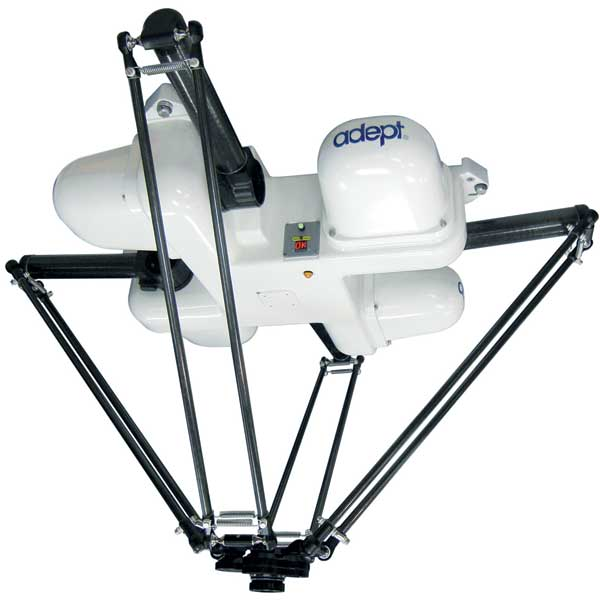
\includegraphics[scale=0.17]{../figures/theadeptquat.jpg}  
	\caption{Robô industrial Adept Quattro}
	\label{fig:Mecanismo}
\end{figure}

Levando-se em conta esta dificuldade de obtenção e a complexidade inerente do modelo dinâmico, o controle de mecanismos de arquitetura paralela é uma tarefa desafiadora. A utilização de estratégias de controle não baseadas em modelo pode deixar muito a desejar na exploração do potencial que estes mecanismos oferecem, principalmente em tarefas de seguimento de trajetória \cite{Chung}, e a utilização de modelos dinâmicos simplificados pode limitar significativamente o desempenho do projeto de controladores baseados em modelo, principalmente quando se trabalha com altas velocidades e acelerações. Além disso, mesmo na hipótese do modelo dinâmico completo estar disponível, o emprego de técnicas de controle não linear pode acarretar um custo  computacional muito elevado \cite{Craig, Slotini, Zubizarreta, Zubizarreta3}. Este paradigma, aliado à escassez de trabalhos publicados com comprovação experimental de técnicas de controle aplicáveis a mecanismos paralelos \cite{Rynaldo}, resulta na exploração insatisfatória dos potenciais promissores de tais máquinas, como resposta dinâmica rápida e alta precisão \cite{Abdellatif}.
	
Com o intuito de atacar os problemas da dificuldade de obter modelos dinâmicos completos e diminuir o custo computacional de suas implementações em leis de controle baseadas em modelos, esta tese propõe um algoritmo genérico de modelagem dinâmica de mecanismos paralelos translacionais, o qual pode ser utilizado para calcular previamente termos do modelo dinâmico em um número finito de pontos do espaço de trabalho, sendo necessário apenas o cálculo de interpolações em tempo real.  Além disso, em virtude de existirem poucos  trabalhos publicados, apresentando comprovação experimental de técnicas de controle aplicáveis a mecanismos paralelos, nesta tese, são obtidos e apresentados resultados experimentais da implementação de 8 diferentes estratégias de controle, tanto baseadas como não baseadas em modelo, incluindo estratégias de controle não linear robusto. Desta maneira, o trabalho desenvolvido nesta tese visa contribuir para uma melhor exploração do grandes potenciais dos mecanismos com este tipo de arquitetura.


%Além disso, atacando o problema da  escassez de trabalhos publicados com comprovação experimental de técnicas de controle aplicáveis a mecanismos paralelos, são obtidos e apresentados resultados experimentais da implementação de 8 diferentes estratégias de controle, tanto baseadas como não baseadas em modelo, incluindo estratégias de controle não linear robusto. Desta maneira, o trabalho desenvolvido nesta tese visa contribuir para uma melhor exploração do grandes potenciais dos mecanismos com este tipo de arquitetura.
    
    %Uma alternativa para a superação desta dificuldade seria a combinação de técnicas de controle não linear robusto (por exemplo, controle por modos deslizantes \cite{Slotini, Utkin}) com modelos dinâmicos completos de mecanismos paralelos, desenvolvidos a partir de novas metodologias de modelagem de sistemas multicorpos \cite{22orsino, Orsino2013, 23orsino, 21orsino}. Com esta estratégia, torna-se possível sintetizar leis de controle de alto desempenho e custo computacional mais adequado, viabilizando uma maior exploração do potencial promissor dos mecanismos paralelos.

%OBJETIVOS E JUSTIFICATIVAS--------------------------------------------
\section{Objetivos}\label{objetivos}

O objetivo geral desta Tese é contribuir para o aumento do desempenho de manipuladores paralelos. Quanto aos objetivos específicos, propõe-se que este aprimoramento seja realizado mediante o emprego de técnicas de controle baseadas em modelo do manipulador. Neste sentido, almeja-se fornecer recomendações quanto à modelagem dinâmica, à técnica de controle mais adequada, bem como a sua implementação.

%Os principais objetivos da tese s\~ao:
%\begin{itemize}
%\item Desenvolvimento de um algoritmo gerador de modelos dinâmicos completos de mecanismos paralelos, de forma implícita. Será utilizada uma metodologia baseada no método Orsino de acoplamento de subsistemas multicorpos \cite{23orsino}.


%\item Elabora\c{c}\~ao de metodologias de projeto de controlador n\~ao linear robusto, de alto desempenho, aplicável a  mecanismos de arquitetura paralela. Para tanto, serão consideradas as incertezas param\'etricas e a possibilidade de atua\c{c}\~ao redundante \cite{Cheng},  além de estratégias para a síntese de leis de controle com custo computacional consideralvemente menor do que as tradicionais, que empregam o Controle por Torque Computado \cite{Craig, Zubizarreta}.

%\item Realizar a modelagem cinemática e dinâmica dos mecanismos 5R \cite{22orsino} e 2\underline{R}SU+\underline{P}PaP \cite{Rynaldo, Kumazawa}, utilizando o algoritmo de modelagem desenvolvido.

%\item Realizar o projeto de um controlador de trajetória para os mecanismos escolhidos, utilizando a metodologia de projeto de controle proposta.

%\item Realizar simula\c{c}\~oes dinâmicas utilizando as leis de controle sintetizadas.

%\item Realizar a validação experimental dos controladores projetados no protótipo dos mecanismos 5R, o qual se encontra no laboratório de mecanismos da EPUSP.
%\end{itemize}

%É importante ressaltar que os 5 primeiros objetivos citados já foram parcialmente alcançados e que a arquitetura paralela 2\underline{R}SU+\underline{P}PaP foi desenvolvida pelo grupo de pesquisa do Prof. Dr. Tarcio Antonio Hess Coelho, havendo ainda poucos estudos na literatura sobre ela. %Sendo assim, pode-se afirmar que simulações dinâmicas e validações experimentais de leis de controle não linear robusto neste mecanismo tem caráter inédito.

%SOBRE A ORGANIZAÇÃO DO TEXTO--------------------------------------------
\section{Sobre a organização do texto}\label{organizacao}

O capítulo 2 apresenta a revisão da Literatura sobre o assunto, sendo que a metodologia da pesquisa é descrita no capítulo 3. A seguir, os capítulos 4 e 5 abordam a modelagem dinâmica de manipuladores seriais e paralelos, respectivamente. Com relação ao projeto dos controladores, este assunto é elaborado no capítulo 6. No capítulo 7 são apresentados os resultados mais relevantes desta Tese, além da pertinente discussão. Por fim, no capítulo 8, apresentam-se as principais conclusões da Tese e os temas sugeridos para pesquisa futura.

%REVISAO--------------------------------------------------------------------
\chapter{Revisão da literatura}\label{revision}

Considerando o tema de pesquisa desta Tese, esta revisão se concentrará em tópicos relacionados à modelagem dinâmica, ao controle e à utilização de bancada de ensaios para validação experimental.


\section{Modelagem dinâmica}

Quando se trata de modelagem dinâmica, os mecanismos seriais possuem características topológicas e cinemáticas que podem ser exploradas para facilitar a geração dos modelos cinemáticos e dinâmicos. Suas estruturas mecânicas correspondem a mecanismos de cadeia aberta, apenas com juntas ativas de um grau de liberdade, rotativas ou prismáticas. Além disso, o número de coordenadas generalizadas coincide com o número de atuadores e com a mobilidade do mecanismo \cite{Craig}. 

De fato, o modelo cinemático pode ser obtido, recursivamente ao longo da cadeia cinemática, pelo emprego de métodos vetoriais ou matriciais, partindo-se da base e se dirigindo ao efetuador \cite{Siciliano}. Tradicionalmente, empregam-se os vetores $\mq$ e $\mx$ para descrever as coordenadas associadas aos atuadores e ao efetuador, respectivamente \cite{Cabral, Carvalho}. Enquanto que o problema direto é de resolução relativamente simples, o problema inverso demanda a realização de um processo mais elaborado. Matematicamente, este corresponde à resolução de um sistema não-linear de equações algébricas. Para algumas topologias que utilizem mecanismos esféricos nos punhos, é possível alcançar o desacoplamento das equações de posição e orientação do efetuador \cite{Waldron}.

Com relação à dinâmica, a geração das equações também pode ser realizada de modo recursivo, partindo-se do efetuador e se dirigindo à base, sendo que a solução do problema inverso é obtida mediante a resolução de um sistema linear de equações algébricas. Por outro lado, a solução do problema dinâmico direto é alcançada pela integração de um sistema de equações diferenciais ordinárias (ODEs) \cite{Featherstone}.

%Não tratar de formalismos clássicos da Mecânica (NE,L,GA etc), apenas citar referências q os descrevam de modo geral (livros, tese Orsino) e de modo específico quando aplicados a manipuladores paralelos (artigos). A seguir, serão tratadas as questões ligadas à topologia dos manipuladores, à geração do modelo, bem como as análises para a sua resolução.



%Neste momento, tratar do manipulador paralelo, sua topologia em comparação com os seriais.

Já quando se trata de mecanismos paralelos, dependendo da complexidade da estrutura, podem existir juntas de 1, 2 ou até 3 graus de liberdade, ativas ou passivas. Além disso, o número de elos geralmente é muito superior. Ao se elaborar o modelo cinemático, é possível notar que haverá um grande número de variáveis, dentre as quais algumas serão consideradas independentes e outras, dependentes \cite{Merlet}.

No início do processo de modelagem, é comum  se realizar um corte nas juntas que conectam o efetuador às cadeias cinemáticas. Deste modo, ocorrerá a decomposição do mecanismo original de cadeia fechada no elo do efetuador e nas demais cadeias. Assim, admite-se que estas cadeias possam ser tratadas como abertas. Consequentemente, as equações cinemáticas, geradas em cada cadeia, expressarão o acoplamento entre as variáveis dependentes e independentes do mecanismo. Além disso, para os manipuladores paralelos, a literatura destaca que o problema inverso da cinemática de posição é menos complexo que o direto \cite{Merlet}. 

Saha e Schielen \cite{Saha} mencionam que a dinâmica inversa, uma vez definida a trajetória do efetuador, determina os esforços dos atuadores necessários para o controle, enquanto que a direta é utilizada em simulações do manipulador com o controlador.

Com relação à dinâmica, Pekal e Fraczek \cite{Pekal2} esclarecem que a solução do problema direto pode ser obtida mediante a resolução de um sistema de equações diferenciais e algébricas (DAEs), representado pelas Eq.(\ref{DAE1}, \ref{DAE2})

\begin{equation}
\mM \, \ddot{\mq} + \mA^\msT \,\mlambda = \meta
\label{DAE1}
\end{equation}
%
\begin{equation}
\bar{\mq} \, (\mq,t) \, = \, \mzr
\label{DAE2}
\end{equation}

Sendo
%\begin{equation}
%\meta = \mu - \mnu - \mg
%\end{equation}
\begin{equation}
\mA(\mq,t) = \frac{\partial \bar{\mq}}{\partial \mq}
\end{equation}

Uma alternativa é resolver o sistema representado pela Eq.(\ref{DAE3}), 

\begin{equation}
\underbrace{\left[ \begin{array}{cc}
\mM & \mA^\msT \\
\mA & \mzr
\end{array}
\right]}_{\mY}
\left[ \begin{array}{c}
\ddot{\mq} \\
\mlambda
\end{array}
\right] =
\left[ \begin{array}{c}
\meta \\
-\mb
\end{array}
\right]
\label{DAE3}
\end{equation}

\vspace{0.5cm}

sendo
\begin{equation}
\mb = \frac{\partial (\mA \dot{\mq})}{\partial \mq} \, \dot{\mq} + 2 \frac{\partial \mA}{\partial t} \, \dot{\mq} + \frac{\partial^2 \bar{\mq}}{\partial t^2}
\end{equation}

Para melhorar a precisão associada às restrições de posição e velocidade, recomenda-se substituir $\mb$ por $\mb'$, expresso na Eq.(\ref{baumgarte}), que é conhecido como método de Baumgarte para a estabilização das restrições \cite{Baumgarte, Featherstone, Nikravesh}, sendo $\hat{\alpha} = \hat{\beta} = 1/t_c$, com  $0.01 \lesssim t_c \lesssim 0.1 $ \cite{Featherstone}. 
%
\begin{equation}
\mb' = \mb + 2\hat{\alpha} \dot{\bar{\mq}} + \hat{\beta}^2 \bar{\mq}
\label{baumgarte}
\end{equation}

%\vspace{0.5cm}

Um outro modo de aprimorar a precisão é alcançado pela separação das coordenadas $\mq$ em dois grupos: independentes $\mq\ssh$ e dependentes $\mq\cir$. Assim, multiplica-se a Eq.(\ref{DAE1}) pelo complemento ortogonal \cite{Kordjazi} de $\mA^\msT$. Pekal e Fraczek \cite{Pekal} discutem várias alternativas de obtenção do complemento ortogonal, dentre elas, destacam-se a decomposição QR, a decomposição em matrizes de autovalores e autovetores e a decomposição em valores singulares (SVD). Com esta ação, eliminam-se os multiplicadores de Lagrange e o número de equações se reduz à mobilidade do mecanismo. Em seguida, utiliza-se de relações cinemáticas para  escrever as acelerações $\ddot{\mq}$ em função de $\ddot{\mq}\ssh$. Por consequência, somente as acelerações e velocidades independentes serão integradas no sistema de equações diferenciais. Além disso, em cada passo de integração, as variáveis dependentes $\mq\cir$ e $\dot{\mq\cir}$ serão calculadas a partir das independentes, estabilizando as restrições de posição e velocidade.

Quando a matriz dos coeficientes $\mY$ , expressa na Eq.(\ref{DAE1}), for singular, os métodos numéricos normalmente empregados, como decomposição LU ou QR, não serão capazes de resolver o sistema de equações. Neste caso, costuma-se empregar $\mY^\msP$, ou seja, a matriz inversa de Moore-Penrose. Outras formulações, como as de Udwadia-Kalaba, Udwadia-Phohomsiri e baseadas no método dos mínimos quadrados, também foram propostas para tratar as situações em que $\mY$ é singular.

Segundo Mariti et al. (2011) \cite{Mariti}, expressar o modelo dinâmico por meio de coordenadas redundantes, independentemente do formalismo escolhido, possui como propósito a realização de simulações de sistemas multicorpos, sendo que um exemplo é o software comercial MSC-Adams. No entanto, se a finalidade for o controle de manipuladores, significando que o modelo é parte integrante de implementações que demandem  cálculos em tempo real, a expresssão das equações dinâmicas nas coordenadas independentes é necessária.

Além disso, é largamente difundido que a escolha das variáveis cinemáticas independentes recaia sobre as componentes do vetor $\mq^\star$, associadas aos deslocamentos impostos pelos atuadores, e suas derivadas temporais. No entanto, alguns autores \cite{Li, Khalil2} mencionam as vantagens de se escolher as componentes do vetor $\mx$, afirmando que a expressão do modelo dinâmico nestas variáveis é menos complexa.

Na literatura, são conhecidas várias formulações para realizar a modelagem dinâmica de sistemas multicorpos, como os formalismos de Newton-Euler, Lagrange, Gibbs-Appel, Maggi, Boltzmann-Hamel, os métodos de Kane e Udwadia-Kalaba, e os princípios dos trabalhos virtuais e potências virtuais \cite{23orsino}. Porém, na literatura de modelagem de mecanismos paralelos, podemos destacar as seguintes formulações como as mais comumente utilizadas:

\begin{itemize}
\item Formalismo de Newton-Euler
\item Formalismo de Lagrange
\item Princípio dos Trabalhos Virtuais e das Potências Virtuais
\item Formulação de Lagrange-D'Alembert
\item Formalismo de Boltzmann-Hamel
\item Método de Kane
\item Formulação do Complemento Ortogonal Natural
\end{itemize}

\subsection{Formalismo de Newton-Euler}

A utilização do formalismo de Newton-Euler é bastante popular para a realização de simulações dinâmicas de mecanismos seriais, tendo em vista que foram desenvolvidos algoritmos recursivos super eficientes para a aplicação deste formalismo neste tipo de arquitetura, como pode ser visto em Featherstone et al. \cite{Featherstone}. Porém, para se beneficiar deste tipo de estratégia em mecanismos paralelos, é necessária a utilização de algoritmos de fechamento de malha, os quais aumentam consideravelmente o custo computacional das simulações. Provavelmente por esta razão, aliada à questão da complexidade de implementação dos algoritmos, não foram encontrados na literatura artigos aplicando esta estratégia na modelagem de mecanismos paralelos. 

Apesar da desvantagem de ter que trabalhar com forças reativas no equacionamento, não é raro encontrar na literatura trabalhos que o utilizem. Dentre estes, podemos citar os trabalhos de Arian et al. \cite{Arian}, Dasgupta et al. \cite{Dasgupta}, Li et al. \cite{LiWang}, Shiau et al. \cite{Shiau} e Zhang et al. \cite{Zhang}.

Em \cite{Arian}, \cite{LiWang} e \cite{Dasgupta}, são feitas a simulações dinâmicas inversas de mecanismos paralelos, de 3 graus de liberdade, nos dois primeiros trabalhos, e de 6 graus de liberdade, no último, utilizando o formalismo de Newton-Euler. Em \cite{Arian} e \cite{LiWang} as simulações são comparadas com \emph{softwares} comerciais. Em \cite{Arian}, também é feita a modelagem utilizando o princípio dos trabalhos virtuais, e são comparados o número de operações e o tempo médio gasto por operação em cada formulação. Como era de se esperar, a formulação do Princípio dos Trabalhos Virtuais se mostrou muito mais eficiente em ambos os quesitos, tendo em vista que não são realizados os cálculos dos esforços reativos. Em \cite{Dasgupta} foi feita uma eliminação de boa parte dos esforços vinculares utilizando manipulações algébricas, o que possibilitou reduzir bastante o custo computacional da simulação.

Em \cite{Shiau} e \cite{Zhang}, os mecanismos paralelos 3-PRS e 3-RRR, respectivamente, são modelados  também utilizando o formalismo de Newton-Euler. Em ambos os trabalhos é considerado o efeito de folgas, e em \cite{Shiau} também o de atritos. A partir dos modelos obtidos, em ambos são feitas simulações dinâmicas diretas. Em \cite{Zhang} é utilizado o método de estabilização de Baumgarte \cite{Baumgarte} para estabilizar a integração numérica. Em \cite{Shiau}, além das simulações, é feita a linearização do modelo dinâmico para determinar as frequências naturais do mecanismo em função da posição do efetuador.

\subsection{Formalismo de Lagrange}

Formulações baseadas na mecânica analítica em geral são muito mais atrativas para realizar a modelagem de mecanismos paralelos, tendo em vista que os esforços vinculares não mais aparecem no equacionamento. Isso justifica a popularidade das escolhas pelo formalismo de Lagrange e pelos princípios dos trabalhos virtuais e das potências virtuais para realizar esta tarefa.

Dentre os trabalhos que utilizam o formalismo de Lagrange, podemos citar os trabalhos de  Li et al. \cite{Li3}, Singh et al. \cite{Singh, Singh2, Singh3} e Yao et al. \cite{Yao}.

Em \cite{Singh}, \cite{Singh2} e \cite{Singh3}, são modelados 3 mecanismos paralelos planos de 3 graus de liberdade utilizando o formalismo de Lagrange. Em todos, são realizadas simulações dinâmicas diretas comparando o desempenho de diversas leis de controle. Apenas em \cite{Singh2} é realizada uma dedução completa do modelo dinâmico mostrando a expressão deduzida do modelo. Curiosamente, são adotadas as coordenadas do efetuador como coordenadas generalizadas, e a dedução se mostra relativamente simples para essa arquitetura escolhida, com essa escolha de variáveis.

Já em \cite{Li3}, um mecanismo paralelo espacial de 3 graus de liberdade é modelado, utilizando o formalismo de Lagrange com multiplicadores e o princípio dos trabalhos virtuais, sendo que no último são utilizadas hipóteses simplificadoras. São realizadas simulações dinâmicas inversas e são comparados os resultados utilizando o modelo completo com os resultados utilizando o modelo simplificado.

Em \cite{Yao}, é feita a simulação dinâmica inversa de um mecanismo ainda mais complexo, de 5 graus de liberdade e atuação redundante, também utilizando o formalismo de Lagrange e métodos de otimização para determinar os esforços. Este trabalho, porém, também mostra muito pouco da dedução. Assim, dados a complexidade do mecanismo e o fato de que não é comentado em lugar nenhum o uso de coordenadas redundantes, imagina-se que o modelo utilizado seja um modelo simplificado.

\subsection{Princípio dos Trabalhos Virtuais e das Potências Virtuais}

Levando-se em conta a revisão feita, não foi percebida uma grande diferença de popularidade entre a utilização dos formalismos de Newton-Euler e Lagrange nos artigos que tratam da modelagem dinâmica de mecanismos paralelos. Porém, uma abordagem que se mostrou extremamente popular foi a utilização das formulações do princípio dos trabalhos virtuais ou do princípio das potências virtuais. Dentre os trabalhos que utilizam estes princípios, podemos citar os trabalhos de Arian et al. \cite{Arian} (já comentado), Codourey et al. \cite{Codourey, CodoureyBurdet}, Gallardo-Alvarado et al. \cite{GallardoAlvarado}, Geike et al. \cite{Geike}, Li et al. \cite{LiStaicu, Li}, Staicu et al. \cite{Staicu, Staicu2, Staicu3, StaicuCarpCiocardia, StaicuLiu, StaicuZhang, StaicuZhangRugescu}, Wu et. al \cite{Wu}, Zhao et al. \cite{Zhao, Zhao2} e  Zhu et al. \cite{Zhu}.

No trabalhos de Codourey et al. \cite{Codourey, CodoureyBurdet} e no de Li et al. \cite{Li}, são modelados mecanismos paralelos de 3 graus de liberdade, do tipo DELTA nos dois primeiros, e do tipo 3-PRS no terceiro, utilizando o princípio dos trabalhos virtuais. São desprezadas as inércias distribuídas dos elos ligados à plataforma, e suas massas são distribuídas entre as duas pontas em que cada elo é ligado, de modo a simplificar o processo de modelagem.

Já em \cite{GallardoAlvarado}, é modelado um robô paralelo de 4 graus de liberdade utilizando a teoria das helicóides e o princípio dos trabalhos virtuais.

Em \cite{Geike}, é proposta uma metodologia de modelagem interessante, na qual já se dividem as coordenadas generalizadas em um conjunto de variáveis dependentes e outro de variáveis independentes, utilizando a relação entre seus deslocamentos virtuais para obter as equações de movimento. A metodologia é utilizada para realizar a simulação dinâmica inversa de dois mecanismos paralelos, um de 3 graus de liberdade e outro de 6. Além disso, é discutida qual é a forma mais eficiente de implementação da metodologia desenvolvida.

Nos trabalhos de Staicu et al. \cite{Staicu, Staicu2, Staicu3, StaicuCarpCiocardia, StaicuLiu, StaicuZhang, StaicuZhangRugescu} e no de Li et al. \cite{LiStaicu} são modelados mecanismos paralelos de 3 graus de liberdade utilizando uma metodologia de modelagem recursiva matricial baseada no princípio dos trabalhos virtuais ou no princípio das potências virtuais, e são realizadas simulações dinâmicas inversas. Esses trabalhos apresentam longos equacionamentos para não precisar recorrer a simplificações; porém, em todos os trabalhos, perto do final da dedução do modelo dinâmico, cita-se que será usada a \emph{equação fundamental da dinâmica de robôs paralelos}, a qual está publicada em \cite{StaicuFrances}. Este artigo, porém, está escrito em francês e é muito difícil de ser encontrado.

Por fim, nos trabalhos de Zhao et al. \cite{Zhao, Zhao2} e de Zhu et al. \cite{Zhu}, são modelados, utilizando o princípio dos trabalhos virtuais e o conceito de jacobianos dos elos, mecanismos paralelos de 6 graus de liberdade nos dois primeiros, e de 3 graus de liberdade no terceiro, sendo que em \cite{Zhao2} o mecanismo possui atuação redundante. Em todos são realizadas simulações dinâmicas inversas.

\subsection{Formulação de Lagrange-D’Alembert}

Além disso, foram encontrados trabalhos que utilizam uma mistura do Princípio dos Trabalhos Virtuais com o formalismo de Lagrange, denominada formulação de Lagrange-D’Alembert, dentre os quais podemos citar o de Cheng et al \cite{ChengLiu} e Yen et al. \cite{Yen}.

O trabalho de Cheng et al \cite{ChengLiu}, pois nele é utilizada a formulação de Lagrange-D’Alembert para deduzir uma formulação de acoplamento de subsistemas. A formulação é utilizada para obter o modelo dinâmico de um mecanismo paralelo de 2 graus de liberdade com atuação redundante. São utilizados os modelos já conhecidos para as cadeias seriais, e é feito o acoplamento dos subsistemas a partir de jacobianos dos vínculos cinemáticos.

Em \cite{Yen}, também é utilizada uma estratégia de acoplamento de subsistemas, também deduzida deduzida a partir formulação de Lagrange-D’Alembert, para obter o modelo dinâmico de um mecanismo paralelo de 3 graus de liberdado. No entanto, neste trabalho, a estratégia não é apresentada de uma maneira mais geral, podendo dar a impressão ao leitor de que isso só foi possível devido à topologia particular do mecanismo em questão. São realizadas simulações dinâmicas diretas do controle de posição do mecanismo, utilizando controladores as técnicas de controle PID e Controle por Torque Computado, as quais são comparadas com resultados experimentais utilizando as mesmas estratégias de controle.

\subsection{Método de Kane}

Uma formulação que é bastante popular na literatura de mecanismos seriais, porém não muito popular na literatura de mecanismos paralelos, é o Método de Kane \cite{Kane}. Dentre os poucos trabalhos que utilizam esta formulação para realizar a modelagem dinâmica de mecanismos paralelos, podemos citar os trabalhos de Ben-Horina et al. \cite{BenHorina} e Shukla et al. \cite{Shukla}.

Em \cite{BenHorina}, é realizada a modelagem dinâmica, utilizando o método de Kane, de um robô paralelo de 6 graus de liberdade, cuja atuação é feita por 3 atuadores planos, os quais apresentam 2 graus de liberdade cada. A modelagem é feita com o auxílio do \emph{software} AUTOLEV. São realizadas simulações dinâmicas inversas do mecanismo proposto, e de mais dois mecanismos de 6 graus de liberdade, para efeito de comparação.

Em \cite{Shukla}, também é realizada a modelagem dinâmica de um mecanismo paralelo de 6 graus de liberdade, uma plataforma de Gough–Stewart, utilizando o método de Kane. São realizadas simulações dinâmicas diretas do controle do mecanismo, considerando a dinâmica dos atuadores, utilizando malhas de controle do tipo PID em cascata e compensadores de atraso.

\subsection{Formalismo de Boltzmann-Hamel}

O Formalismo de Boltzmann-Hamel \cite{Jarzebowska} também não se mostrou muito popular na literatura de modelagem dinâmica de mecanismos paralelos. Dentre os trabalhos encontrados, podemos citar os trabalhos de Abdellatif et al. \cite{Abdellatif2} e o de Altuzarra et al. \cite{20altuzarra}.

Tanto em \cite{Abdellatif2} quanto em \cite{20altuzarra}, são utilizadas as equações de Boltzmann-Hamel para a deduzir formulações que permitem a obtenção do modelo dinâmico explícito de mecanismos paralelos através dos modelos das cadeias seriais, do efetuador, e jacobianos dos vínculos cinemáticos. Em \cite{20altuzarra}, é utilizada a formulação proposta para obter o modelo dinâmico do mecanismo 3-PRS. Em \cite{Abdellatif2} são apresentadas simulações dinâmicas inversa e direta, sendo esta última com leis de controle baseadas no modelo, de um mecanismo paralelo de 6 graus de liberdade.


\subsection{Formulação do Complemento Ortogonal Natural}

A formulação do Complemento Ortogonal Natural foi proposta por Angeles et al. em \cite{Angeles}. Sua principal idéia é projetar as equações dinâmicas de cada corpo rígido do sistema em um espaço ortogonal às reações vinculares. Este procedimento é realizado através da obtenção de um complemento ortogonal ao jacobiano das equações de vínculo obtido através de relações cinemáticas dos \emph{twists} de cada corpo com um conjunto de quasi-velocidades independentes. Formulações similares são bastante exploradas por Orsino et al. em \cite{22orsino}, e generalizadas em \cite{23orsino}. Dentre os trabalhos que utilizam esta formulação, podemos citar os trabalhos de Akbarzadeh et al. \cite{Akbarzadeh}, Khan et al. \cite{Khan} e Xi et al. \cite{Xi}.

Em \cite{Akbarzadeh}, é descrita uma metodologia genérica de modelagem dinâmica multi-corpos utilizando a formulação do Complemento Ortogonal Natural. Basicamente são obtidos os modelos dinâmicos desacoplados de cada corpo rígido, utilizando a formulação de Newton-Euler, e é feito o acomplamento das equações dinâmicas através do uso do Complemento Ortogonal Natural. A metodologia proposta é aplicada em um mecanismo paralelo esférico do tipo SST e são realizadas simulações dinâmicas inversa e direta do mecanismo.

Em \cite{Xi}, é realizada a modelagem dinâmica de um mecanismo paralelos de 6 graus de liberdade, do tipo hexapod, utilizando a formulação do Complemento Ortogonal Natural. São realizadas simulações dinâmicas inversas do mecanismos em altas e baixas velocidades.

Por fim, em \cite{Khan}, é proposta uma metodologia recursiva de modelagem baseada na formulação do Complemento Ortogonal Natural. A metodologia proposta é utilizada para a obtenção do modelo dinâmico de uma mecanismo paralelo plano do tipo 3-RRR, realizando primeiro a modelagem dinâmica das cadeias seriais, e acoplando-as utilizando o Complemento Ortogonal Natural. Também é realizada a simulação dinâmica inversa do mecanismo, utilizando o modelo obtido.








%%%%%%%%%%%%%%%%%%%%%%%%%%%%%%%%%%%%%%%%%%%%%%%%%%%%%%%%%%%%%%%%%%%%%

\section{Controle}

Existem diversas técnicas propostas pela literatura para realizar o controle de mecanismos paralelos. Dentre elas, podemos destacar:

\begin{itemize}
\item Controle Proporcional-Integral-Derivativo (PID)
\item Controle por Torque Computado (CTC)
\item Controle por Torque Computado com pré-alimentação (CTCp)
\item Controle por Torque Computado Estendido (CTCe)
\item Controle Preditivo Baseado em Modelo (CPM)
\item Controle Adaptativo
\item Controle por Modos Deslizantes (CMD)
\end{itemize}

A técnica mais simples consiste na utilização de malhas do tipo PID, controlando cada junta ativa de maneira independente, considerando a dinâmica do mecanismo como distúrbios de controle. Essa técnica é caracterizada por sua facilidade de projeto e implementação, tanto em hardware quanto em software, além de exibir um desempenho satisfatório para movimento lento. Porém, essa técnica não se mostra adequada para a realização de trajetórias em altas velocidades e/ou acelerações \cite{Honegger, Zubizarreta}.

Uma das técnicas de controle mais exploradas na literatura é o Controle por Torque Computado (CTC). Basicamente, é uma técnica de controle não linear, mais conhecida como linearização pela realimentação, aplicada a sistemas mecânicos. A técnica consiste na utilização de duas malhas de controle, uma malha que realiza o desacoplamento do sistema e a compensação das não linearidades, e outra malha composta por PIDs independentes \cite{Craig}. Como resultado, alcança-se um desempenho  superior  àquele obtido utilizando simples PIDs, permitindo inclusive a realização de trajetórias precisas em altas velocidades e/ou acelerações. No entanto, seu desempenho poderá ser limitado pela qualidade/fidelidade do modelo dinâmico utilizado para a compensação das não linearidades \cite{SlotiniSMC}. Sua implementação também é mais complexa, visto que é necessário calcular o modelo dinâmico inverso em tempo real, o que também aumenta consideravelmente seu custo computacional. Além disso, a técnica é sensível a incertezas estruturadas (paramétricas) e não estruturadas (dinâmicas não modeladas). Como exemplos de utilização do CTC, podem ser citados os trabalhos de Cheng at al. \cite{Cheng}, Li e Wu \cite{Li}, Li e Fu \cite{Li2}, Shang at al. \cite{Shang} e Yen at al. \cite{Yen}.

\begin{figure}[h]
	\centering
	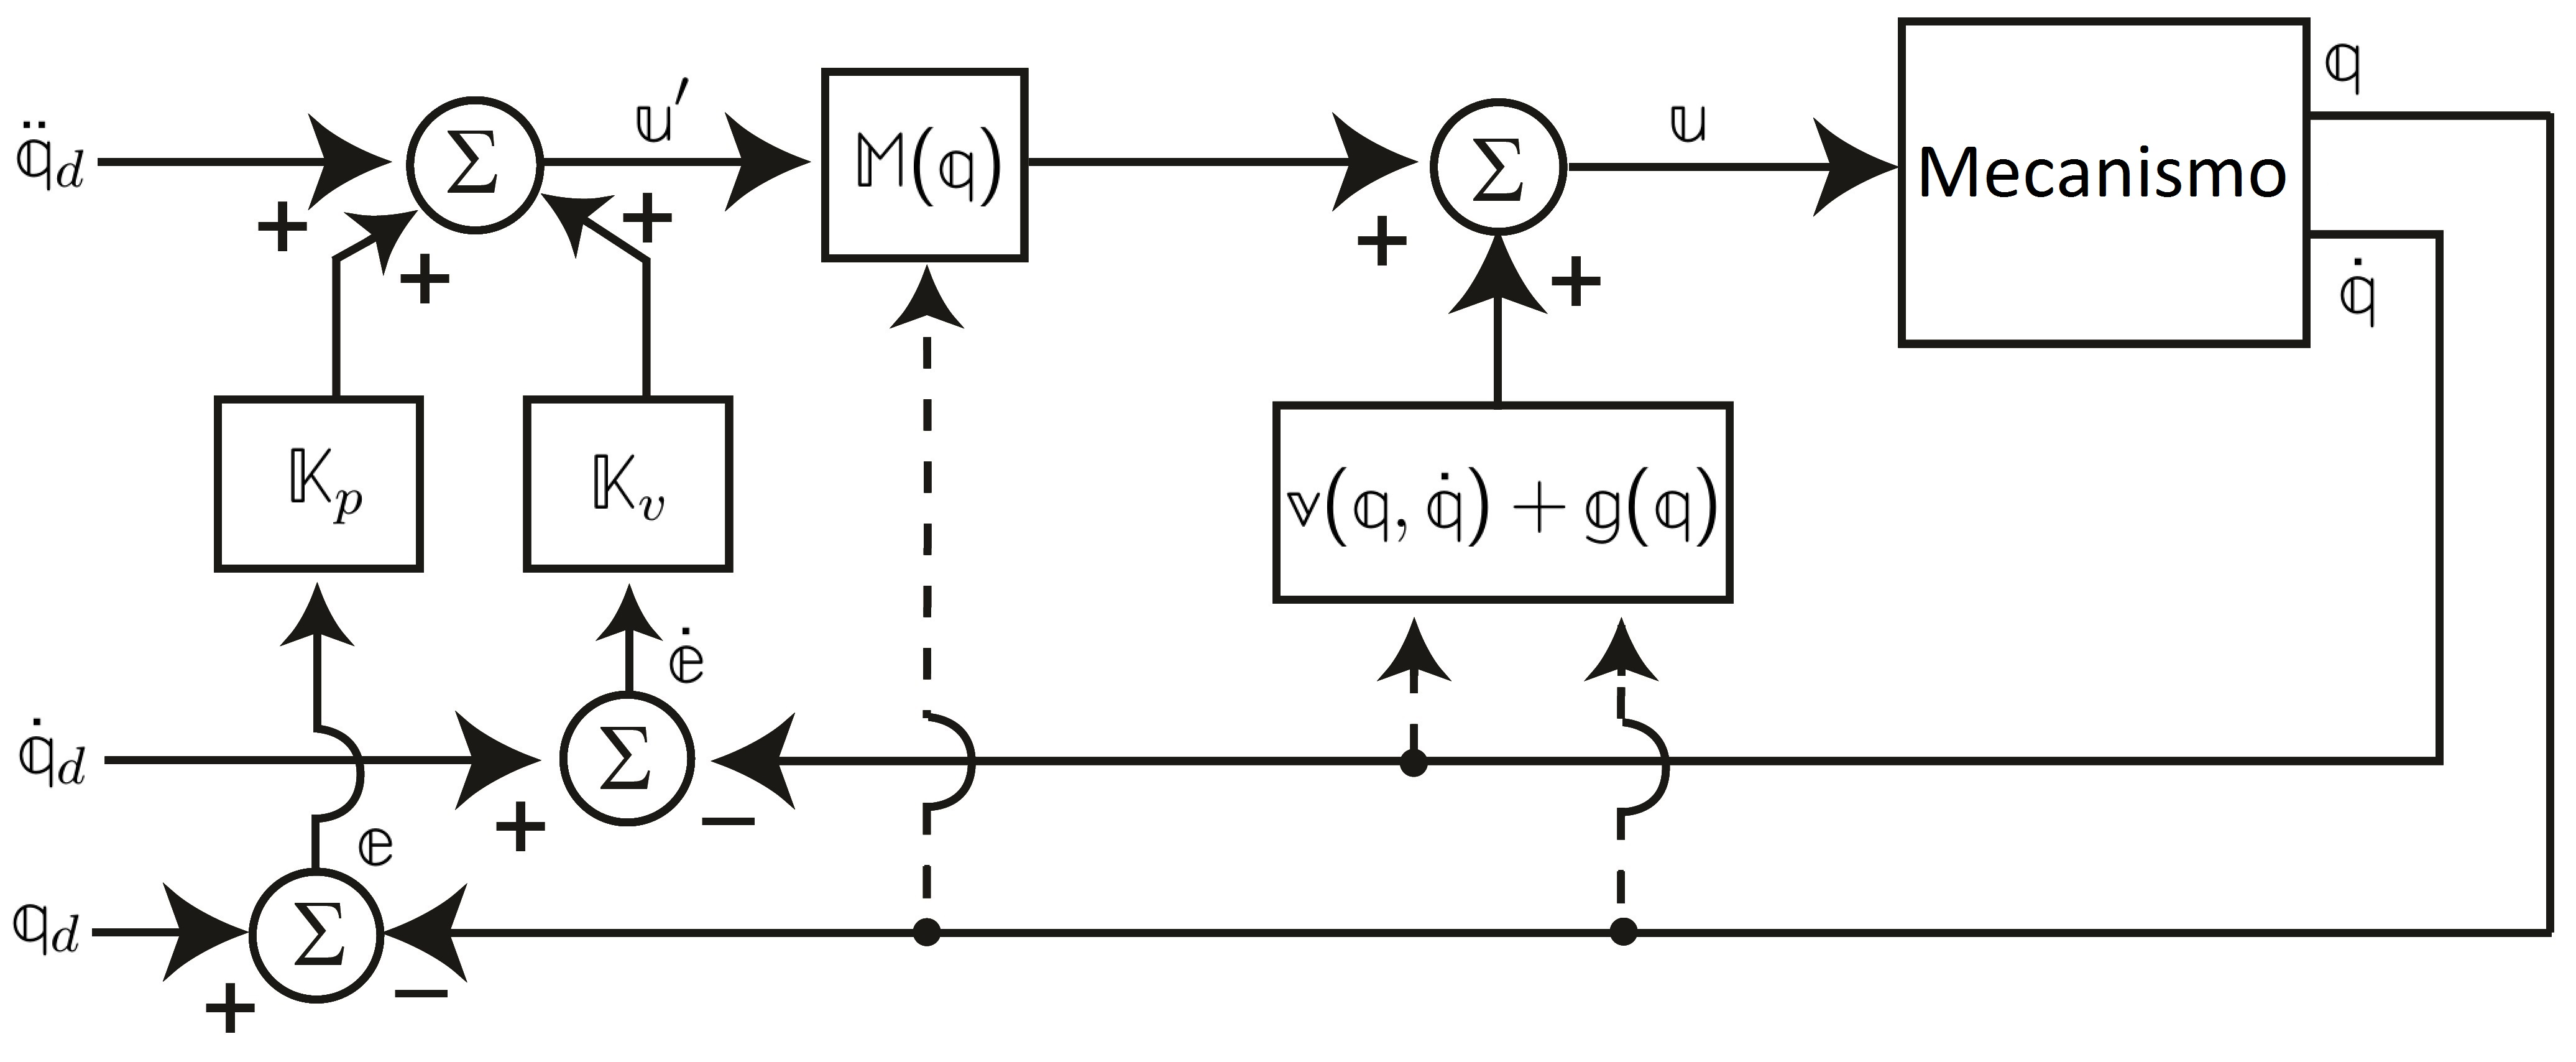
\includegraphics[scale=0.385]{../figures/CTC.jpg}  
	\caption{Malha de CTC (Adaptado de \cite{Craig})}
	\label{fig:CTC}
\end{figure}

Visando a redução do custo computacional associado ao cálculo do modelo dinâmico em tempo real, alguns autores propõe a utilização do CTC com pré-alimentação (CTCp) \cite{Khalil, Siciliano, Spong}. Essa técnica é similar ao CTC, com a diferença de que a compensação das não linearidades é feita por pré-alimentação e não mais por realimentação.  Consequentemente, realiza-se o cálculo do modelo dinâmico previamente, diminuindo o custo computacional.

De fato, Codourey \cite{Codourey} obteve uma redução de 600\% no erro de posição utilizando o CTCp em um ensaio experimental com o robô DELTA, ao substituir os PDs originais. Na simulação do controle de um mecanismo 6-UPS, Wang et al. \cite{Wang} utilizaram em cascata controladores lineares de posição, velocidade e corrente em cada junta ativa, além de  uma compensação dinâmica por pré-alimentação dos distúrbios de torque.

\begin{figure}[h]
	\centering
	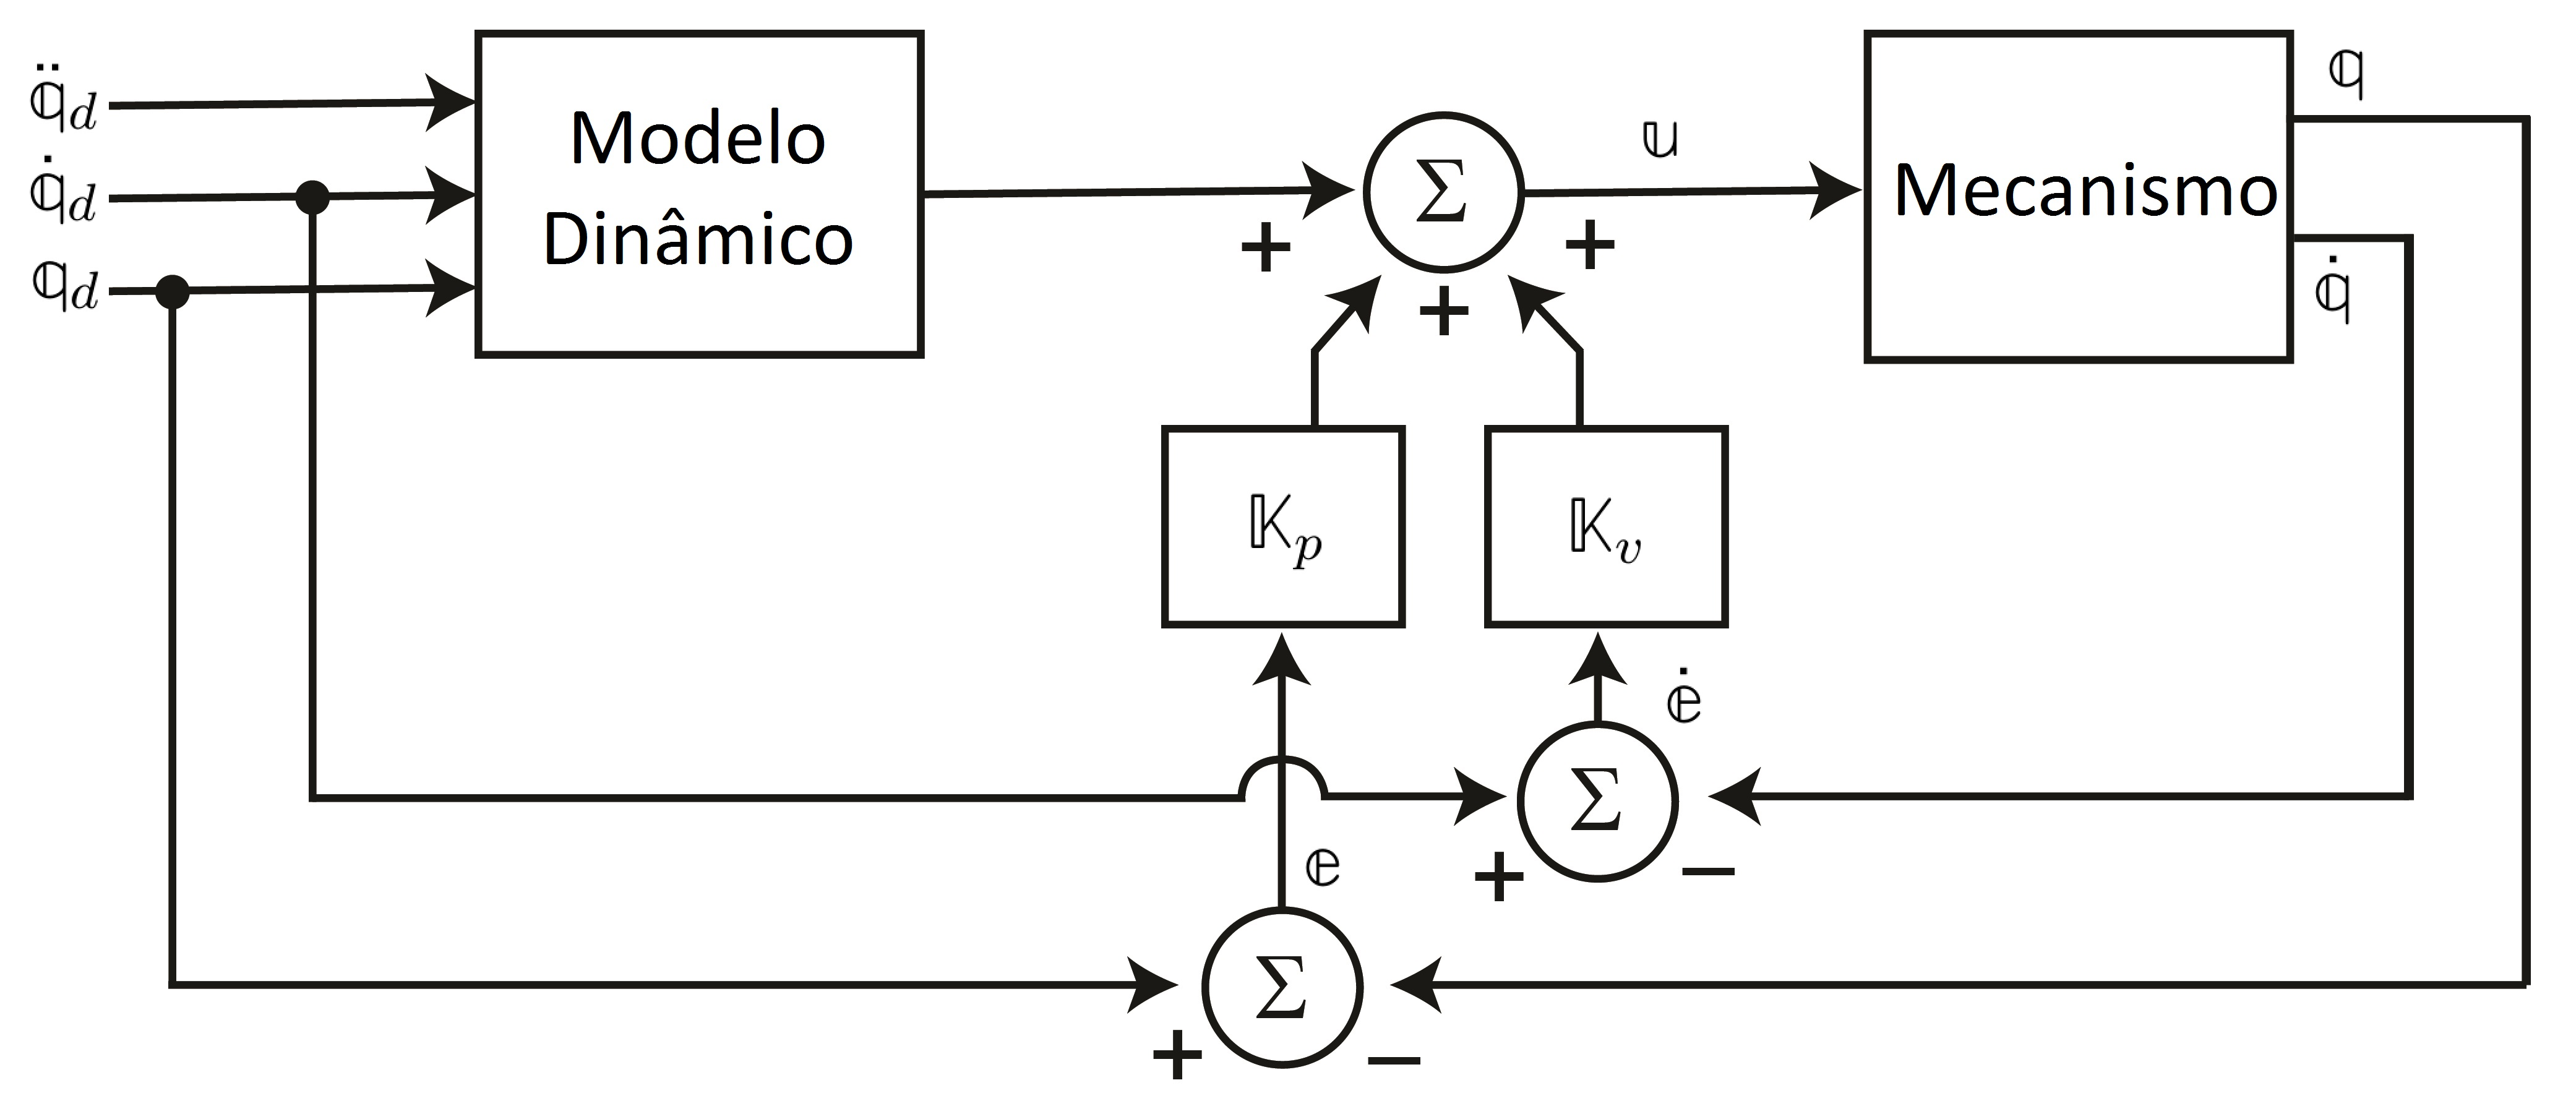
\includegraphics[scale=0.385]{../figures/CTCp.jpg}  
	\caption{Malha de CTCp (Adaptado de \cite{Craig})}
	\label{fig:CTCp}
\end{figure}

Com o intuito de melhorar a robustez do CTC associada a incertezas paramétricas, Zubizarreta et al. \cite{Zubizarreta, Zubizarreta2, Zubizarreta3, Zubizarreta4} propuseram  o  Controle por Torque Computado Estendido (CTCe), que utiliza informação redundante obtida pelo sensoriamento de juntas passivas. Em \cite{Zubizarreta}, os controladores propostos demonstraram maior robustez, principalmente em relação a parâmetros cinemáticos, durante as simulações realizadas com o mecanismo 3-RRR.

Outra técnica alternativa, aplicada a mecanismos paralelos, é o controle preditivo baseado em modelo (CPM). Para a sua implementação, o CPM necessita minimizar uma função objetivo, dependente das saídas e do esforço de controle, ambos calculados em tempo futuro \cite{Camacho}. Assim, dependendo do modelo utilizado, o processo de otimização pode agregar um custo computacional que inviabilize o controle, comprometendo a motivação inicial de aprimorar o desempenho do sistema. Como exemplos de utilização do CPM, podem ser citados os trabalhos de Vivas et al. \cite{Vivas} e   Duchaine et al. \cite{Duchaine}.

Com o propósito de controlar o mecanismo H4, Vivas et al. \cite{Vivas} utilizaram  uma malha de CPM linear e outra malha para compensação das não linearidades. Após a comparação do desempenho do controlador proposto com  o CTC, os autores observaram maior robustez do CPM a incertezas paramétricas. 

Duchaine et al. \cite{Duchaine}, por sua vez, propuseram um controlador preditivo baseado no modelo não linear de um mecanismo paralelo de 6 graus de liberdade. Visando a obtenção de uma solução analítica para o problema de otimização, foram adotadas diversas hipóteses simplificadoras no modelo dinâmico do mecanismo. Com o intuito de comparar o controlador proposto com um PID, foram feitos alguns experimentos, onde se observou  que o CPM apresentou erro nulo de posição no final da trajetória, enquanto que o PID demorou um tempo considerável para alcançar erro nulo. Foi verificada a equivalência entre o custo computacional dos 2 controladores. 

O controle adaptativo, também encontrado na literatura, caracteriza-se pela utilização de leis de adaptação para realizar a estimação em tempo real de parâmetros do sistema ou de termos de compensação dinâmica. Sendo assim, as técnicas de controle adaptativo possibilitam que o sistema se torne praticamente insensível a incertezas paramétricas. Para o caso em que se realiza a estimação em tempo real dos parâmetros do sistema, pode-se dizer que o custo computacional é superior ao do CTC, visto que é necessário integrar as leis de adaptação em tempo real. Além disso, é necessário obter o modelo dinâmico linear em relação aos parâmetros do sistema \cite{SlotiniA}, o que pode ser uma tarefa difícil, inviabilizando, em alguns casos, a aplicação da técnica. Em \cite{Codourey2} é proposto um algoritmo de obtenção do modelo dinâmico simplificado de mecanismos paralelos nesse formato.

Em \cite{SlotiniA} é proposta uma lei de controle que combina o controle adaptativo com a técnica de controle robusto conhecida por Controle por Modos Deslizantes. Chemori et al. \cite{Chemori} utilizaram essa técnica  com o intuito de diminuir os erros de posição em regime permanente no controle de um mecanismo paralelo do tipo PAR2. Por outro lado, Honegger at al. \cite{Honegger} empregaram o controle adaptativo com estimação em tempo real dos parâmetros do sistemas, realizando a compensação dinâmica por pré-alimentação, em um mecanismo  paralelo do tipo Hexaglide.

\begin{figure}[h]
	\centering
	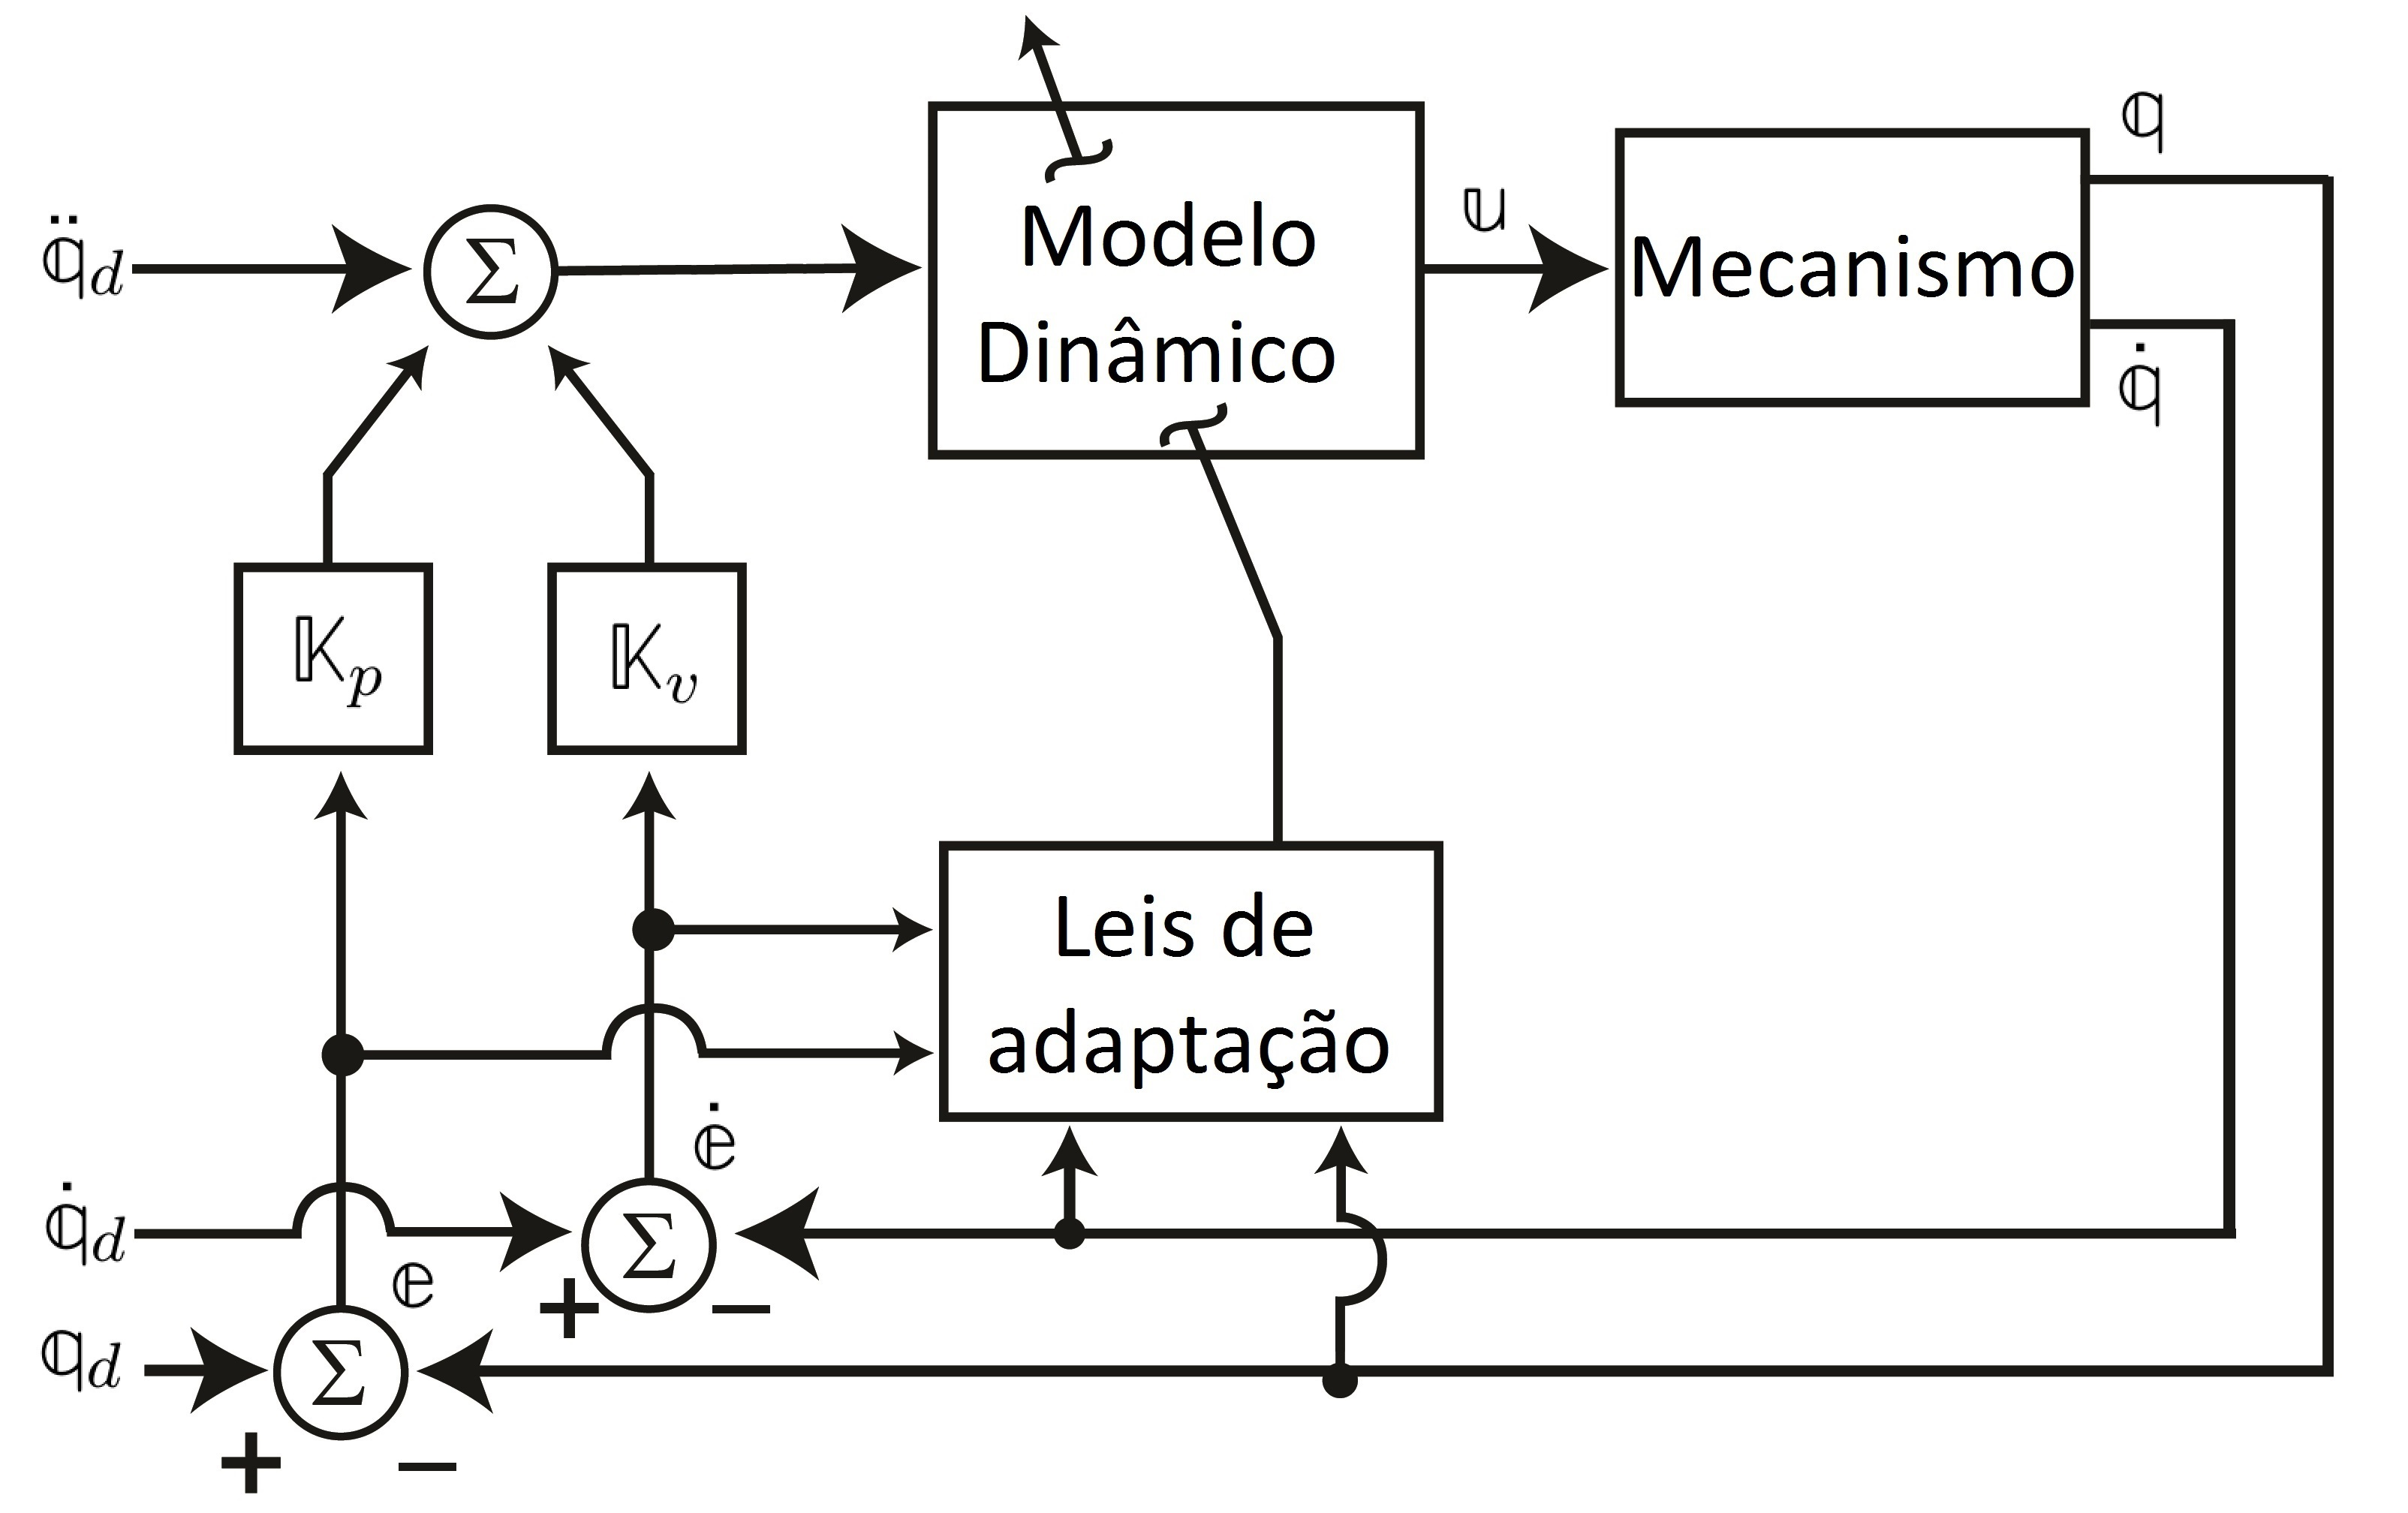
\includegraphics[scale=0.385]{../figures/CA.jpg}  
	\caption{Malha de controle adaptativo (Adaptado de \cite{Craig})}
	\label{fig:CA}
\end{figure}

Outra técnica promissora para aplicação em mecanismos paralelos é o Controle por Modos Deslizantes (CMD). A técnica consiste no projeto de leis de controle que levem o sistema para superfícies de escorregamento no espaço de fase, de modo que assim que o sistema atinje e é mantido nas superfícies de escorregamento, o erro de controle decai exponencialmente para zero \cite{Slotini}. Para garantir que o sistema atinja em tempo finito e se mantenha nas superfícies de escorregamento, são utilizados termos descontínuos na lei de controle, o que pode causar problemas de oscilações bruscas em alta frequência nos esforços de controle ({\em chattering}). Em \cite{Guldner}  e  \cite{Utkin2} são propostas técnicas para evitar esse tipo de problema. A grande vantagem da utilização deste tipo de lei de controle é sua grande robustez a incertezas estruturadas e não estruturadas, sendo possível realizar o projeto do controlador de modo a suprimir um dado nível de incertezas paramétricas. Em \cite{SlotiniSMC} é proposta uma metodologia de projeto de Controle por Modos Deslizantes para manipuladores robóticos seriais.

Na literatura são encontradas diversos artigos utilizando a técnica de CMD aliada à lógica {\em fuzzy} e/ou redes neurais para o controle de manipuladores robóticos \cite{Begon, Ertugrul, Hu, Sadati}. Begon et al. \cite{Begon} propuseram uma lei de controle baseada na teoria de CMD e na utilização de lógica {\em fuzzy} para controlar de maneira independente os atuadores de um mecanismo paralelo do tipo Hexa. A técnica proposta teve o intuito de obter a robustez característica do CDM sem necessitar de uma lei de controle com termos descontínuos, evitando o {\em chattering}.

Em \cite{Zeinali}, Zeinali et al. desenvolveram uma lei de controle  baseada nas teorias de CMD e controle adaptativo. O controlador desenvolvido realiza a compensação dinâmica em tempo real do erro de modelagem através de uma lei de adaptação. Além disso, substitui o termo descontínuo da lei de controle por um termo do tipo PID, com o intuito de evitar o {\em chattering}. A estabilidade e robustez da lei de controle proposta foram provadas utilizando a teoria de estabilidade de Lyapunov \cite{Slotini}. A robustez da lei de controle foi verificada através de simulações do controlador proposto aplicado a um mecanismo serial do tipo \underline{R}\underline{R}, nas quais o controlador conseguiu manter erros de posição muito pequenos em regime permanente, mesmo sendo baseado em um modelo muito pobre e na presença de distúrbios de torque. A técnica apresentada se mostra promissora, porém, como no artigo foi feita apenas a simulação da lei de controle em um mecanismo serial bidimensional, ainda não se pode afirmar nada sobre seu desempenho em mecanismos paralelos tridimensionais.

\section{Bancada de ensaios}

%METODOLOGIA--------------------------------------------------------------------
\chapter{Metodologia da Pesquisa}\label{method}

Fundamentalmente, a metodologia desta pesquisa compreende a execução de seis fases, abrangendo desde o desenvolvimento de algoritmos para as modelagens cinemática e dinâmica ao projeto de controladores e sua validação experimental.

\section{Primeira fase} 
Desenvolver um algoritmo genérico, capaz de gerar os modelos dinâmicos completos de mecanismos paralelos que operem em espaço plano, esférico ou tridimensional. Esta geração parte da definição da topologia do mecanismo paralelo, suas cadeias cinemáticas, descrevendo a localização relativa de seus elos e juntas. 

Dentre os efeitos de modelagem considerados, destacam-se os decorrentes da inércia efetiva e acoplada, das forças de Coriolis e centrífugas, da força gravitacional, bem como dos esforços dos atuadores. Pretende-se que a geração dos modelos seja realizada de forma implícita. Para tanto, será empregado o método Recursivo Modular de Modelagem (RMM) proposto por Orsino \cite{23orsino} que, por meio da definição de níveis hierárquicos da estrutura de um sistema mecânico e a descrição da dependência das variáveis cinemáticas envolvidas,  permite o acoplamento de subsistemas multicorpos.

\section{Segunda fase} 
Efetuar as modelagens cinemática e dinâmica do mecanismo articulado plano 5R \cite{22orsino}, utilizando o algoritmo desenvolvido na fase anterior.

\section{Terceira fase} 
Nesta fase, diferentes técnicas de controle serão avaliadas sob a perspectiva de sua utilização em manipuladores paralelos. Assim, 
em princípio, esta pesquisa foca na síntese de um controlador não-linear robusto e de alto desempenho. Para tanto, serão consideradas as incertezas paramétricas e a possibilidade de atuação redundante \cite{Cheng}, além de estratégias para a determinação de leis de controle com custo computacional
consideralvemente menor do que as tradicionais, que empreguem o Controle por Torque Computado \cite{Craig, Zubizarreta}.

\section{Quarta fase} Avaliar o emprego de diferentes técnicas de controle de trajetória aplicadas especificamente para o manipulador 5R,
empregando a metodologia da terceira fase.

\section{Quinta fase} Realizar diversas simulações que permitam observar a consistência dos resultados, no tocante às análises cinemáticas direta e inversa, bem como das análises dinâmicas direta e inversa. Além disso, serão determinadas as respostas dinâmicas do manipulador sujeito às distintas leis de controle sintetizadas.

\section{Sexta fase} 
De modo a avaliar o desempenho previsto pelo uso de diferentes controladores para o manipulador paralelo 5R, será realizada a validação experimental em uma das bancadas de ensaio do LaMMaR. Para tanto, serão escolhidas duas trajetórias: uma que considere o comportamento em regime permanente e outra em regime transitório. 

Neste sentido, almeja-se observar se haverá alguma diferença de desempenho se o controle for executado no espaço das juntas ou no da tarefa. Além disso, pretende-se considerar os efeitos da implementação de técnicas de controle puras ou combinadas.
Para auxiliar na comparação entre as técnicas de controle, serão definidas duas métricas: uma que considere o erro de posicionamento do efetuador e outra a magnitude dos torques dos atuadores.

%\section{O que tinha antes} 
%O estágio atual de desenvolvimento do presente projeto ocorre basicamente em três áreas:
%aplicação do algoritmo de modelagem e simulação para os mecanismos 5R \cite{22orsino} e 2\underline{R}SU + \underline{P}PaP \cite{Kumazawa}, o projeto e simulação de controladores não lineares robustos de alto desempenho baseado no modelo dinâmico para os mecanismos citados, e a validação experimental das leis de controle sintetizadas.

%Os trabalhos no âmbito de modelagem e simulação estão sendo desenvolvidos a partir da aplicação do algoritmo de modelagem cinemática e dinâmica de mecanismos paralelos desenvolvido, baseado na utilização dos parâmetros de Denavit-Hartenberg \cite{Craig, Denavit, Lipkin} e no método Orsino de acoplamento de subsistemas \cite{23orsino}. Toda modelagem será feita em C++, utilizando uma biblioteca otimizada de cálculo matricial (Armadillo).
%As simulações da dinâmica direta do mecanismo serão feitas utilizando o método Runge-Kutta de 8ª ordem \cite{RK} para solução de sistemas de EDOs, de modo a garantir estabilidade numérica do método, mesmo utilizando leis de controle quase descontínuas.

%Os trabalhos na área de projeto de controle serão feitos utilizando a metodologia desenvolvida de projeto de controladores robustos multivariáveis para mecanismos paralelos, baseada no modelo dinâmico do mecanismo a ser controlado e na técnica de controle por modos deslizantes \cite{Slotini, Utkin}.

%Os trabalhos no âmbito da validação experimental das leis de controle sintetizadas serão realizados no protótipo do mecanismo 5R que encontra-se no laboratório de mecanismos. A bancada experimental do mecanismo 5R já está funcional e já forem realizados alguns testes de leis de controle de trajetória baseadas no modelo dinâmico do mecanismo. Para a realização da validação experimental nesta bancada, será realizada a identificação dos parâmetros do sistema e suas respectivas incertezas, projeto do controlador baseado nos parâmetros e incertezas identificadas, implementação das leis de controle, e aquisição de dados. \\

\begin{figure}[h]
	\centering
	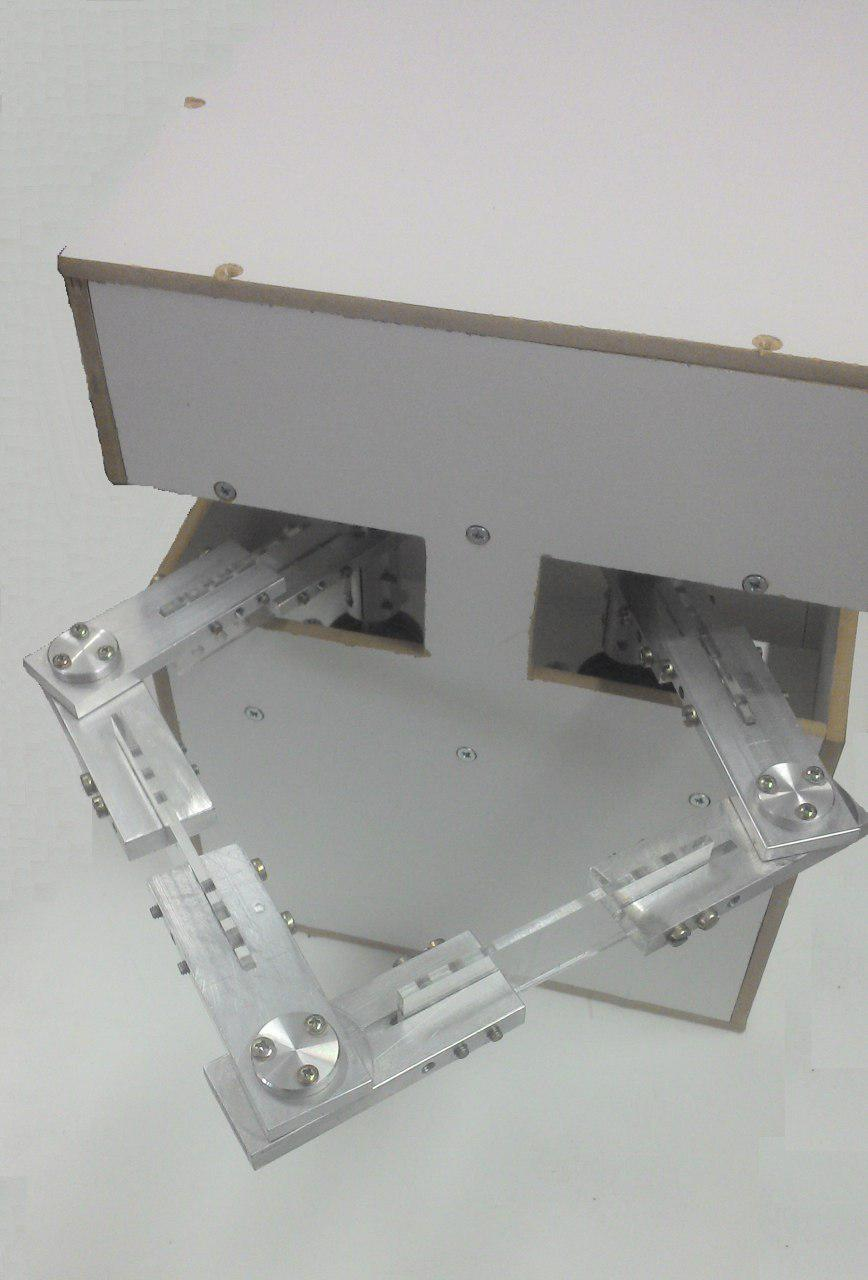
\includegraphics[scale=0.3]{../figures/Clara.jpg}  
	\caption{Protótipo do mecanismo 5R}
	\label{fig:Mecanismo2}
\end{figure}

%MODELAGEM DE MANIPULADORES SERIAIS--------------------------------------------

\part{Modelagem}
	
\chapter{Modelagem de manipuladores seriais}
\capepigrafe[0.5\textwidth]{``Não é que eu goste de complicar as coisas, elas é que gostam de ser complicadas comigo''}{Lewis Carroll}

Este capítulo tem o intuito de apresentar um algoritmo genérico para a obtenção do modelo cinemático e dinâmico de mecanismos seriais. O algoritmo apresentado é implementável em linguagens de programação comumente usadas atualmente, como C++, Java e Python, sem necessitar de recursos de manipulação simbólica. \\
Para a obtenção do modelo, são necessários apenas os parametros de Denavit-Hartemberg \cite{Craig, Denavit, Lipkin, Cabral} do mecanismo e as posições dos centros de massa dos ligamentos em relação aos sistemas de coordenadas fixos aos ligamentos. \\ 

Seja $\ssB$ um sistema mecânico serial de $\nu$ graus de liberdade. Primeiramente, fazemos as seguintes definições:

\begin{itemize}
\item $\llN$ ou $\llB_0$: referencial inercial.
\item $\ttN$ ou $\ttB_0$: sistema de coordenadas da base do mecanismo, fixo a $\llN$.
\item $\llB_i, \,i=1,...,\nu$: i-ésimo ligamento.
\item $\ttB_i, \,i=1,...,\nu$: sistema de coordenadas solid\'ario a $\llB_i$.
\item $\tto_i, \,i=0,...,\nu$: origem do sistema $\ttB_i$.
\item $\{\vi_i, \vj_i, \vk_i\}, \,i=0,...,\nu$: base ortonormal do sistema $\ttB_i$.
\item $\ttg_i, \,i=1,...,\nu$: centro de massa de $\llB_i$.
\item $\ttx$: ponto no espa\c{c}o fixo ao efetuador.
\item $m_i$: massa da barra $\llB_i$.
\item $\vI_{\ttg_i}$: tensor de in\'ercia da barra $\llB_i$ em relação a seu centro de massa.
\item $\mI_i$: tensor de in\'ercia $\vI_{\ttg_i}$ escrito na base $\ttN$, ou seja, $\vct{\vI_{\ttg_i}}_{\ttN \rl \ttN}$.
\item $q_i, \,i=1,...,\nu$: deslocamento relativo (angular ou linear) da i-ésima junta.
\item  $\mq$: matriz-coluna de $\nu$ coordenadas generalizadas independentes. É dada por $\mq = \begin{bmatrix}
q_1 & ... & {q}_{\nu}
\end{bmatrix}^\msT $.
\item $\vg$: Vetor aceleração gravitacional.
\item $\mgamma$: Vetor aceleração gravitacional escrito na base $\ttN$, ou seja, $\vct{\vg}_{\ttN}$.
\item $\vf_i$: Vetor força não-reativa resultante aplicada no centro de massa de $\llB_i$.
\item $\vtau_i$: Vetor torque não-reativo resultante aplicado em $\llB_i$.
\item $\overline{\mf}_i$: Matriz-coluna de forças não-reativas generalizadas aplicadas no subsistema $\llB_i$. É dada por $\overline{\mf}_i = \begin{bmatrix}
\vct{\vf_i}_\ttN^\msT &
\vct{\vtau_i}_\ttN^\msT
\end{bmatrix}^\msT $.
\end{itemize}

\section{Cinemática}

\subsection{Cinemática de posição}

Dados os parâmetros de Denavit-Hartemberg $a_i$, $\alpha_i$, $d_i$ e $\theta_i$, com $1 \leq i \leq \nu$, é possível obter as matrizes de transformação homogênea $\hvct{\vone}_{\ttB_{i-1} \rl \ttB_i}$ a partir da seguinte expressão \cite{Cabral} :

\begin{empheq}[box=\myyellowbox]{equation} \label{eq:TransformacaoHomogeneaDH}
\hvct{\vone}_{\ttB_{i-1} \rl \ttB_i} =
\begin{bmatrix}
\ccos\theta_i & -\ssin\theta_i \ccos\alpha_i &  \ssin\theta_i \ssin\alpha_i & a_i\ccos\theta_i \\
\ssin\theta_i &  \ccos\theta_i \ccos\alpha_i & -\ccos\theta_i \ssin\alpha_i & a_i\ssin\theta_i \\
0             &  \ssin\alpha_i               &  \ccos\alpha_i               & d_i \\
0             & 0                            & 0                            & 1
\end{bmatrix},\, i=1,...,\nu
\end{empheq}

Tendo obtido $\hvct{\vone}_{\ttB_{i-1} \rl \ttB_i}$, é possível obter as transformações homogêneas que relacionam os sistemas solidários aos ligamentos ($\ttB_i$) ao sistema da base ($\ttN$) pela seguinte expressão recursiva:

\begin{empheq}[box=\myyellowbox]{equation} \label{eq:H__}
\hvct{\vone}_{\ttN \rl \ttB_i} =
\begin{cases}
\hvct{\vone}_{\ttB_0 \rl \ttB_1}, \text{se } i=1 \\
\hvct{\vone}_{\ttN \rl \ttB_{i-1}} \cdot \hvct{\vone}_{\ttB_{i-1} \rl \ttB_i}  , \text{se } i>1
\end{cases} \, i=1,...,\nu
\end{empheq}

As matrizes  $\hvct{\vone}_{\ttN \rl \ttB_i}$ apresentam o seguinte formato:
\begin{empheq}[box=\lightbluebox]{equation} \label{eq:H__2}
\hvct{\vone}_{\ttN \rl \ttB_i} =
\begin{bmatrix}
\vct{\vi_{i}}_{\ttN} & \vct{\vj_{i}}_{\ttN} & \vct{\vk_{i}}_{\ttN} & \vct{\tto_i}_{\ttN} \\
0 & 0 & 0 & 1
\end{bmatrix}
\end{empheq}

Sendo assim, tendo obtido $\hvct{\vone}_{\ttN \rl \ttB_i}$, automaticamente obtemos $\vct{\vi_{i}}_{\ttN}, \vct{\vj_{i}}_{\ttN}, \vct{\vk_{i}}_{\ttN}$ e $\vct{\tto_i}_{\ttN}$. Note que também obtemos as coordenadas do efetuador no sistema da base, pois
\begin{empheq}[box=\myyellowbox]{equation} \label{eq:x_}
\vct{\ttx}_{\ttN} = \vct{\tto_{\nu}}_{\ttN}
\end{empheq}

Além disso, como $\vct{\ttg_i}_{\ttB_i}$ são dados de entrada do algoritmo, obtemos as coordenadas dos centros de massa dos ligamentos no sistema da base através da seguinte expressão:
\begin{empheq}[box=\myyellowbox]{equation} \label{eq:og__}
\hvct{\ttg_i}_{\ttN} = \hvct{\vone}_{\ttN \rl \ttB_i} \cdot \hvct{\ttg_i}_{\ttB_i}
\end{empheq}

\subsection{Cinemática de velocidades lineares}

A velocidade do efetuador pode ser obtida aplicando recursivamente o príncipio da composição de movimentos para velocidades lineres deduzido anteriormente \eqref{eq:Composicao_vel}:

\begin{equation}
\vv_{\ttx}^{\lllB_0} = \vv_{\ttx \rl \lllB_1}^{\lllB_0} + \vv_{\ttx}^{\lllB_1}
\end{equation}
\begin{equation}
\vv_{\ttx}^{\lllB_1} = \vv_{\ttx \rl \lllB_2}^{\lllB_1} + \vv_{\ttx}^{\lllB_2}
\end{equation}
$$ \vdots $$
\begin{equation}
\vv_{\ttx}^{\lllB_{i-1}} = \vv_{\ttx \rl \lllB_i}^{\lllB_{i-1}} + \vv_{\ttx}^{\lllB_i}
\end{equation}
$$ \vdots $$
\begin{equation}
\vv_{\ttx}^{\lllB_{\nu-1}} = \vv_{\ttx \rl \lllB_\nu}^{\lllB_{\nu-1}} + \vv_{\ttx}^{\lllB_\nu}
\end{equation}

Como $\ttx$ é fixo a $\llB_\nu$, temos que:
\begin{equation}
\vv_{\ttx}^{\lllB_\nu} = \vzr
\end{equation}

Sendo assim, a velocidade do efetuador em relação a cada um dos referenciais pode ser obtida recursivamente pela seguinte expressão:
%\begin{equation}
%\vv_{\ttx}^{\lllB_{i-1}} =
%\begin{cases}
%\displaystyle\sum_{j=i}^{\nu} \vv_{\ttx \rl \lllB_{j}}^{\lllB_{j-1}}, \; 1 \leq i \leq \nu \\
%\vzr, \;\;\;\;\;\;\;\;\;\;\;\; i = \nu + 1
%\end{cases}\, i=1,...,\nu+1
%\end{equation}
\begin{equation}
\vv_{\ttx}^{\lllB_{i-1}} =
\begin{cases}
\vzr, \;\;\;\;\;\;\;\;\;\;\;\;\;\;\; i = \nu + 1 \\
\vv_{\ttx}^{\lllB_{i}} + \vv_{\ttx \rl \lllB_{i}}^{\lllB_{i-1}}, \; 1 \leq i \leq \nu \\
\end{cases}\, i=\nu+1,...,1
\end{equation}



Sendo que, a partir da equação \eqref{eq:Poisson_v}, a velocidade de arrastamento de cada uma das juntas é dada por:
\begin{equation}
\vv_{\ttx \rl \lllB_{i}}^{\lllB_{i-1}} = 
\begin{cases}
\dot{q}_{i} \vk_{i-1}, \;\;\;\;\;\;\;\;\;\;\;\;\;\; \text{i-ésima junta prismática} \\
\dot{q}_{i} \vk_{i-1} \wedge \vr_{\tto_{i-1} \rl \ttx}, \; \text{i-ésima junta rotativa}
\end{cases}\, i=1,...,\nu
\end{equation}

Fazendo as seguintes definições:
\begin{empheq}[box=\myyellowbox]{equation} \label{eq:jvi_}
\mj_{v\,i}(\mq) = \begin{cases}
\vct{\vk_{i-1}}_{\ttN}, \;\;\;\;\;\;\;\;\;\;\;\;\;\;\;\;\;\;\;\;\;\;\;\;\;\;\; \text{i-ésima junta prismática} \\
\vct{\vk_{i-1}}_{\ttN}\wedge (\vct{\ttx}_{\ttN}-\vct{\tto_{i-1}}_{\ttN}) , \; \text{i-ésima junta rotativa} \\
\end{cases} \, i=1,...,\nu
\end{empheq}

\begin{empheq}[box=\lightbluebox]{equation}
\mv_i = \vct{\vv_{\ttx}^{\lllB_{i}} }_{\ttN}
\end{empheq}

\begin{empheq}[box=\lightbluebox]{equation}
\mv^\star  = \mv_0 =\vct{\vv_{\ttx}^{\lllN} }_{\ttN}
\end{empheq}

Temos que:
\begin{equation}
\vct{\vv_{\ttx \rl \lllB_{i}}^{\lllB_{i-1}} }_{\ttN} = \mj_{v\,i} \dot{q}_{i}, \; i=1,...,\nu
\end{equation}
\begin{empheq}[box=\myyellowbox]{equation}
\mv_{i-1} =
\begin{cases}
\mzr, \;\;\;\;\;\;\;\;\;\;\;\;\; i = \nu + 1 \\
\mv_i + \mj_{v\,i}  \dot{q}_{i}, \; 1 \leq i \leq \nu \\
\end{cases}\, i=\nu+1,...,1
\end{empheq}

\begin{empheq}[box=\lightbluebox]{equation}\label{eq:vel_est}
\mv^\star (\mq, \dot{\mq}) = \mJ_v(\mq) \cdot \dot{\mq}
\end{empheq}

Sendo:
\begin{empheq}[box=\myyellowbox]{equation} \label{eq:Jv_}
\mJ_v(\mq) = \begin{bmatrix}
\mj_{v\,1}(\mq) & ... & \mj_{v\,\nu}(\mq)
\end{bmatrix}
\end{empheq}

Para obter as velocidades dos centros de massa dos ligamentos, seguimos a mesma linha de raciocínio e obtemos os seguintes resultados:

Definindo:
\begin{empheq}[box=\myyellowbox]{equation} \label{eq:jvij_}
\mj_{v\,i,j}(\mq) = \begin{cases}
\mzr, \;\;\;\;\;\;\;\;\;\;\;\;\;\;\;\;\;\;\;\;\;\;\;\;\;\;\;\;\;\;\;\;\;\;\;\;\; j>i \\
\vct{\vk_{j-1}}_{\ttN}, \;\;\;\;\;\;\;\;\;\;\;\;\;\;\;\;\;\;\;\;\;\;\;\;\;\;\;\; j\leq i  \text{ e j-ésima junta prismática} \\
\vct{\vk_{j-1}}_{\ttN}\wedge (\vct{\ttg_i}_{\ttN}-\vct{\tto_{j-1}}_{\ttN}) , \; j\leq i \text{ e j-ésima junta rotativa} \\
\end{cases} \, i,j=1,...,\nu
\end{empheq}

\begin{empheq}[box=\lightbluebox]{equation}
\mv_{i,j} = \vct{\vv_{\ttg_i}^{\lllB_{j}}}_{\ttN}
\end{empheq}

\begin{empheq}[box=\lightbluebox]{equation}
\mv^\star_i  = \mv_{i,0} = \vct{\vv_{\ttg_i}^{\lllN} }_{\ttN}
\end{empheq}

Temos:
\begin{empheq}[box=\myyellowbox]{equation} 
\mv_{i,j-1} =
\begin{cases}
\mzr, \;\;\;\;\;\;\;\;\;\;\;\;\;\;\;\;\; j = i+1 \\
\mv_{i,j} + \mj_{v\,i,j} \dot{q}_{j}, \; 1 \leq j \leq i \\
\end{cases}\, i=1,...,\nu, \, j=i+1,...,1
\end{empheq}

\begin{empheq}[box=\lightbluebox]{equation}  \label{eq:v_star_i}
\mv^\star_i(\mq, \dot{\mq}) = \mJ_{v\,i}(\mq) \cdot \dot{\mq}
\end{empheq}

Sendo:
\begin{empheq}[box=\myyellowbox]{equation} \label{eq:Jvi_}
\mJ_{v\,i}(\mq) = \begin{bmatrix}
\mj_{v\,i,1}(\mq) & ... & \mj_{v\,i,\nu}(\mq)
\end{bmatrix}
\end{empheq}

\subsection{Cinemática de velocidades angulares}

A velocidade angular do efetuador pode ser obtida aplicando recursivamente o príncipio da composição de movimentos para velocidades angulares deduzido anteriormente \eqref{eq:composicao_w}:

\begin{equation}
\vomega_{\lllB_\nu}^{\lllB_0} = \vomega_{\lllB_1}^{\lllB_0} + \vomega_{\lllB_\nu}^{\lllB_1}
\end{equation}
\begin{equation}
\vomega_{\lllB_\nu}^{\lllB_1} = \vomega_{\lllB_2}^{\lllB_1} + \vomega_{\lllB_\nu}^{\lllB_2}
\end{equation}
$$ \vdots $$
\begin{equation}
\vomega_{\lllB_\nu}^{\lllB_{i-1}} = \vomega_{\lllB_i}^{\lllB_{i-1}} + \vomega_{\lllB_\nu}^{\lllB_i}
\end{equation}
$$ \vdots $$
\begin{equation}
\vomega_{\lllB_\nu}^{\lllB_{\nu-2}} = \vomega_{\lllB_{\nu-1}}^{\lllB_{\nu-2}} + \vomega_{\lllB_\nu}^{\lllB_{\nu-1}}
\end{equation}


Sendo assim, a velocidade angular do efetuador em relação a cada um dos referenciais pode ser obtida recursivamente pela seguinte expressão:
%\begin{equation}
%\vomega_{\lllB_\nu}^{\lllB_{i-1}} =
%\begin{cases}
%\displaystyle\sum_{j=i}^{\nu} \vomega_{\lllB_{j}}^{\lllB_{j-1}}, \; 1 \leq i \leq \nu \\
%\vzr, \;\;\;\;\;\;\;\;\;\;\;\; i = \nu + 1
%\end{cases}\, i=1,...,\nu+1
%\end{equation}
\begin{equation}
\vomega_{\lllB_\nu}^{\lllB_{i-1}} =
\begin{cases}
\vzr, \;\;\;\;\;\;\;\;\;\;\;\;\;\;\;\; i = \nu + 1 \\
\vomega_{\lllB_\nu}^{\lllB_{i}} + \vomega_{\lllB_{i}}^{\lllB_{i-1}}, \; 1 \leq i \leq \nu \\
\end{cases}\, i=\nu+1,...,1
\end{equation}



Sendo que a velocidade angular de arrastamento de cada uma das juntas é dada por:
\begin{equation}
\vomega_{\lllB_{i}}^{\lllB_{i-1}} = 
\begin{cases}
\vzr, \;\;\;\;\;\;\; \text{i-ésima junta prismática} \\
\dot{q}_{i} \vk_{i-1}, \; \text{i-ésima junta rotativa}
\end{cases}\, i=1,...,\nu
\end{equation}

Fazendo as seguintes definições:
\begin{empheq}[box=\myyellowbox]{equation}  \label{eq:jwi_}
\mj_{\omega\,i}(\mq) = \begin{cases}
\mzr, \;\;\;\;\;\;\;\; \text{i-ésima junta prismática} \\
\vct{\vk_{i-1}}_{\ttN} , \text{i-ésima junta rotativa} \\
\end{cases} \, i=1,...,\nu
\end{empheq}

\begin{empheq}[box=\lightbluebox]{equation}
\momega_i = \vct{\vomega_{\lllB_\nu}^{\lllB_{i}} }_{\ttN}
\end{empheq}

\begin{empheq}[box=\lightbluebox]{equation}
\momega^\star = \momega_0 = \vct{\vomega_{\lllB_\nu}^{\lllN} }_{\ttN} 
\end{empheq}

Temos que:
\begin{equation}
\vct{\vomega_{\lllB_{i}}^{\lllB_{i-1}} }_{\ttN} = \mj_{\omega\,i} \dot{q}_{i}, \; i=1,...,\nu
\end{equation}

\begin{empheq}[box=\myyellowbox]{equation}
\momega_{i-1} =
\begin{cases}
\mzr, \;\;\;\;\;\;\;\;\;\;\;\;\;\; i = \nu + 1 \\
\momega_i + \mj_{\omega\,i} \dot{q}_{i}, \; 1 \leq i \leq \nu \\
\end{cases}\, i=\nu+1,...,1
\end{empheq}

\begin{empheq}[box=\lightbluebox]{equation} \label{eq:vel_ang_est}
\momega^\star(\mq, \dot{\mq}) = \mJ_\omega (\mq) \cdot \dot{\mq}
\end{empheq}

Sendo:
\begin{empheq}[box=\myyellowbox]{equation} \label{eq:Jw_}
\mJ_\omega(\mq) = \begin{bmatrix}
\mj_{\omega\,1}(\mq) & ... & \mj_{\omega\,\nu}(\mq)
\end{bmatrix}
\end{empheq}

Para obter as velocidades angulares de cada ligamentos, seguimos a mesma linha de raciocínio e obtemos os seguintes resultados:

Definindo:
\begin{empheq}[box=\myyellowbox]{equation} \label{eq:jwij_}
\mj_{\omega\,i,j}(\mq) = \begin{cases}
\mzr, \;\;\;\;\;\;\;\;\,  j>i \\
\mj_{\omega\,j}(\mq), \;  j\leq i \\
\end{cases} \, i,j=1,...,\nu
\end{empheq}

\begin{empheq}[box=\lightbluebox]{equation}
\momega_{i,j} = \vct{\vomega_{\lllB_i}^{\lllB_{j}}}_{\ttN}
\end{empheq}

\begin{empheq}[box=\lightbluebox]{equation}
\momega^\star_i = \momega_{i,0} = \vct{\vomega_{\lllB_i}^{\lllN} }_{\ttN} 
\end{empheq}

Temos:
\begin{empheq}[box=\myyellowbox]{equation}
\momega_{i,j-1} =
\begin{cases}
\mzr, \;\;\;\;\;\;\;\;\;\;\;\;\;\;\;\;\;\; j = i+1 \\
\momega_{i,j} + \mj_{\omega\,i,j} \dot{q}_{j}, \; 1 \leq j \leq i \\
\end{cases}\, i=1,...,\nu, \, j=i+1,...,1
\end{empheq}

\begin{empheq}[box=\lightbluebox]{equation} \label{eq:omega_star_i}
\momega^\star_i (\mq, \dot{\mq}) = \mJ_{\omega\,i}(\mq) \cdot \dot{\mq}
\end{empheq}

Sendo:

\begin{empheq}[box=\myyellowbox]{equation} \label{eq:Jwi_}
\mJ_{\omega\,i}(\mq) = \begin{bmatrix}
\mj_{\omega\,i,1}(\mq) & ... & \mj_{\omega\,i,\nu}(\mq)
\end{bmatrix}
\end{empheq}

\subsection{Cinemática de acelerações lineares}

A aceleração do efetuador pode ser obtida aplicando recursivamente o príncipio da composição de movimentos para velocidades lineres deduzido anteriormente \eqref{eq:Composicao_ace}:

\begin{equation}
\va_{\ttx}^{\lllB_0} = \va_{\ttx \rl \lllB_1}^{\lllB_0} + \va_{\ttx}^{\lllB_1} + 2 \vomega_{\lllB_1}^{\lllB_0} \wedge \vv_{\ttx}^{\lllB_1}
\end{equation}
\begin{equation}
\va_{\ttx}^{\lllB_1} = \va_{\ttx \rl \lllB_2}^{\lllB_1} + \va_{\ttx}^{\lllB_2} + 2 \vomega_{\lllB_2}^{\lllB_1} \wedge \vv_{\ttx}^{\lllB_2}
\end{equation}
$$ \vdots $$
\begin{equation}
\va_{\ttx}^{\lllB_{i-1}} = \va_{\ttx \rl \lllB_i}^{\lllB_{i-1}} + \va_{\ttx}^{\lllB_i} + 2 \vomega_{\lllB_i}^{\lllB_{i-1}} \wedge \vv_{\ttx}^{\lllB_i}
\end{equation}
$$ \vdots $$
\begin{equation}
\va_{\ttx}^{\lllB_{\nu-1}} = \va_{\ttx \rl \lllB_\nu}^{\lllB_{\nu-1}} + \va_{\ttx}^{\lllB_\nu} + 2 \vomega_{\lllB_\nu}^{\lllB_{\nu-1}} \wedge \vv_{\ttx}^{\lllB_\nu}
\end{equation}

Como $\ttx$ é fixo a $\llB_\nu$, temos que:
\begin{equation}
\va_{\ttx}^{\lllB_\nu} = \vzr
\end{equation}

Sendo assim, a aceleração do efetuador em relação a cada um dos referenciais pode ser obtida recursivamente pela seguinte expressão:
%\begin{equation}
%\vv_{\ttx}^{\lllB_{i-1}} =
%\begin{cases}
%\displaystyle\sum_{j=i}^{\nu} \vv_{\ttx \rl \lllB_{j}}^{\lllB_{j-1}}, \; 1 \leq i \leq \nu \\
%\vzr, \;\;\;\;\;\;\;\;\;\;\;\; i = \nu + 1
%\end{cases}\, i=1,...,\nu+1
%\end{equation}
\begin{equation}
\va_{\ttx}^{\lllB_{i-1}} =
\begin{cases}
\vzr, \;\;\;\;\;\;\;\;\;\;\;\;\;\;\;\;\;\;\;\;\;\;\;\;\;\;\;\;\;\;\;\;\;\;\;\;\; i = \nu + 1 \\
\va_{\ttx}^{\lllB_i} +\va_{\ttx \rl \lllB_i}^{\lllB_{i-1}} + 2 \vomega_{\lllB_i}^{\lllB_{i-1}} \wedge \vv_{\ttx}^{\lllB_i}, \; 1 \leq i \leq \nu \\
\end{cases}\, i=\nu+1,...,1
\end{equation}



Sendo que, a partir da equação \eqref{eq:Poisson_a}, a aceleração de arrastamento de cada uma das juntas é dada por:
\begin{equation}
\va_{\ttx \rl \lllB_{i}}^{\lllB_{i-1}} = 
\begin{cases}
\ddot{q}_{i} \vk_{i-1}, \;\;\;\;\;\;\;\;\;\;\;\;\;\;\;\;\;\;\;\;\;\;\;\;\;\;\;\;\;\;\;\;\;\;\;\;\;\;\;\;\;\;\;\;\;\;\;\;\;\;\; \text{i-ésima junta prismática} \\
\ddot{q}_{i} \vk_{i-1} \wedge \vr_{\tto_{i-1} \rl \ttx} + \dot{q}^2_{i} \vk_{i-1} \wedge \vk_{i-1} \wedge \vr_{\tto_{i-1} \rl \ttx} , \; \text{i-ésima junta rotativa}
\end{cases}\, i=1,...,\nu
\end{equation}

Fazendo as seguintes definições:
\begin{empheq}[box=\lightbluebox]{equation}
\ma_i = \vct{\va_{\ttx}^{\lllB_{i}} }_{\ttN}
\end{empheq}

\begin{empheq}[box=\lightbluebox]{equation}
\ma^\star = \ma_0 =\vct{\va_{\ttx}^{\lllN} }_{\ttN}
\end{empheq}

Temos que:
\begin{equation}
\vct{\va_{\ttx \rl \lllB_{i}}^{\lllB_{i-1}} }_{\ttN} = \ddot{q}_{i} \mj_{v\,i} + \dot{q}^2_{i} \mj_{\omega\,i} \wedge \mj_{v\,i}, \; i=1,...,\nu
\end{equation}

\begin{empheq}[box=\myyellowbox]{equation}
\ma_{i-1} =
\begin{cases}
\mzr, \;\;\;\;\;\;\;\;\;\;\;\;\;\;\;\;\;\;\;\;\;\;\; i = \nu + 1 \\
\ma_i +  \mj_{v\,i} \ddot{q}_{i} + (\underaccent{\sim}{\ma})_i  , \; 1 \leq i \leq \nu \\
\end{cases}\, i=\nu+1,...,1
\end{empheq}

\begin{empheq}[box=\lightbluebox]{equation} \label{eq:ace_est}
\ma^\star (\mq,\dot{\mq},\ddot{\mq}) = \mJ_v (\mq)  \cdot \ddot{\mq} + \underaccent{\sim}{\ma} (\mq,\dot{\mq})
\end{empheq}

Sendo:
\begin{empheq}[box=\myyellowbox]{equation}
(\underaccent{\sim}{\ma})_i = \dot{q}_{i} \mj_{\omega\,i} \wedge ( \dot{q}_{i}  \mj_{v\,i} + 2  \mv_i)
\end{empheq}

\begin{empheq}[box=\myyellowbox]{equation} \label{eq:a_til}
\underaccent{\sim}{\ma} = \sum_{i=1}^\nu (\underaccent{\sim}{\ma})_i
\end{empheq}

Para obter as acelerações dos centros de massa dos ligamentos, seguimos a mesma linha de raciocínio e obtemos os seguintes resultados:

Definindo:
\begin{empheq}[box=\lightbluebox]{equation}
\ma_{i,j} = \vct{\va_{\ttg_i}^{\lllB_{j}}}_{\ttN}
\end{empheq}

\begin{empheq}[box=\lightbluebox]{equation}
\ma^\star_i = \ma_{i,0} = \vct{\va_{\ttg_i}^{\lllN} }_{\ttN}
\end{empheq}

Temos:
\begin{empheq}[box=\myyellowbox]{equation}
\ma_{i,j-1} =
\begin{cases}
\mzr, \;\;\;\;\;\;\;\;\;\;\;\;\;\;\;\;\;\;\;\;\;\;\;\;\;\;\;\; j = i+1 \\
\ma_{i,j} + \mj_{v\,i,j} \ddot{q}_{j} + (\underaccent{\sim}{\ma}_i)_j, \; 1 \leq j \leq i \\
\end{cases}\, i=1,...,\nu, \, j=i+1,...,1
\end{empheq}

\begin{empheq}[box=\lightbluebox]{equation} \label{eq:a_star_i}
\ma^\star_i (\mq,\dot{\mq},\ddot{\mq}) = \mJ_{v\,i}(\mq) \cdot \ddot{\mq} + \underaccent{\sim}{\ma}_i (\mq,\dot{\mq})
\end{empheq}

Sendo:
\begin{empheq}[box=\myyellowbox]{equation}
(\underaccent{\sim}{\ma}_i)_j = \dot{q}_{j} \mj_{\omega\,i,j} \wedge ( \dot{q}_{j} \mj_{v\,i,j} + 2  \mv_{i,j})
\end{empheq}

\begin{empheq}[box=\myyellowbox]{equation}
\underaccent{\sim}{\ma}_i (\mq, \dot{\mq}) = \sum_{j=1}^i (\underaccent{\sim}{\ma}_i)_j
\end{empheq}

\subsection{Cinemática de acelerações angulares}

A aceleração angular do efetuador pode ser obtida aplicando recursivamente o príncipio da composição de movimentos para acelerações deduzido anteriormente \eqref{eq:composicao_dw}:

\begin{equation}
\dot{\vomega}_{\lllB_\nu}^{\lllB_0} = \dot{\vomega}_{\lllB_1}^{\lllB_0} + \dot{\vomega}_{\lllB_\nu}^{\lllB_1} +  \vomega_{\lllB_1}^{\lllB_0} \wedge \vomega_{\lllB_\nu}^{\lllB_1}
\end{equation}
\begin{equation}
\dot{\vomega}_{\lllB_\nu}^{\lllB_1} = \dot{\vomega}_{\lllB_2}^{\lllB_1} + \dot{\vomega}_{\lllB_\nu}^{\lllB_2} +  \vomega_{\lllB_2}^{\lllB_1} \wedge \vomega_{\lllB_\nu}^{\lllB_2}
\end{equation}
$$ \vdots $$
\begin{equation}
\dot{\vomega}_{\lllB_\nu}^{\lllB_{i-1}} = \dot{\vomega}_{\lllB_i}^{\lllB_{i-1}} + \dot{\vomega}_{\lllB_\nu}^{\lllB_i} +  \vomega_{\lllB_i}^{\lllB_{i-1}} \wedge \vomega_{\lllB_\nu}^{\lllB_i}
\end{equation}
$$ \vdots $$
\begin{equation}
\dot{\vomega}_{\lllB_\nu}^{\lllB_{\nu-2}} = \dot{\vomega}_{\lllB_{\nu-1}}^{\lllB_{\nu-2}} + \dot{\vomega}_{\lllB_\nu}^{\lllB_{\nu-1}} + \vomega_{\lllB_{\nu-1}}^{\lllB_{\nu-2}} \wedge \vomega_{\lllB_\nu}^{\lllB_{\nu-1}}
\end{equation}


Sendo assim, a aceleração angular do efetuador em relação a cada um dos referenciais pode ser obtida recursivamente pela seguinte expressão:
%\begin{equation}
%\vv_{\ttx}^{\lllB_{i-1}} =
%\begin{cases}
%\displaystyle\sum_{j=i}^{\nu} \vv_{\ttx \rl \lllB_{j}}^{\lllB_{j-1}}, \; 1 \leq i \leq \nu \\
%\vzr, \;\;\;\;\;\;\;\;\;\;\;\; i = \nu + 1
%\end{cases}\, i=1,...,\nu+1
%\end{equation}
\begin{equation}
\dot{\vomega}_{\lllB_\nu}^{\lllB_{i-1}} =
\begin{cases}
\vzr, \;\;\;\;\;\;\;\;\;\;\;\;\;\;\;\;\;\;\;\;\;\;\;\;\;\;\;\;\;\;\;\;\;\;\;\;\; i = \nu + 1 \\
\dot{\vomega}_{\lllB_i}^{\lllB_{i-1}} + \dot{\vomega}_{\lllB_\nu}^{\lllB_i} +  \vomega_{\lllB_i}^{\lllB_{i-1}} \wedge \vomega_{\lllB_\nu}^{\lllB_i}, \; 1 \leq i \leq \nu \\
\end{cases}\, i=\nu+1,...,1
\end{equation}



Sendo que a aceleração angular de arrastamento de cada uma das juntas é dada por:
\begin{equation}
\dot{\vomega}_{\lllB_{i}}^{\lllB_{i-1}} = 
\begin{cases}
\vzr, \;\;\;\;\;\;\; \text{i-ésima junta for prismática} \\
\ddot{q}_{i} \vk_{i-1}, \; \text{i-ésima junta rotativa}
\end{cases}\, i=1,...,\nu
\end{equation}

Fazendo as seguintes definições:
\begin{empheq}[box=\lightbluebox]{equation}
\dot{\momega}_i = \vct{\dot{\vomega}_{\ttx}^{\lllB_{i}} }_{\ttN}
\end{empheq}

\begin{empheq}[box=\lightbluebox]{equation}
\dot{\momega}^\star = \dot{\momega}_0 = \vct{\dot{\vomega}_{\lllB_\nu}^{\lllN} }_{\ttN}
\end{empheq}

Temos que:
\begin{equation}
\vct{\dot{\vomega}_{\lllB_{i}}^{\lllB_{i-1}} }_{\ttN} = \ddot{q}_{i} \mj_{\omega\,i} , \; i=1,...,\nu
\end{equation}

\begin{empheq}[box=\myyellowbox]{equation}
\dot{\momega}_{i-1} =
\begin{cases}
\mzr, \;\;\;\;\;\;\;\;\;\;\;\;\;\;\;\;\;\;\;\;\;\;\;\;\; i = \nu + 1 \\
\dot{\momega}_i +  \mj_{\omega\,i} \ddot{q}_{i} + (\underaccent{\sim}{\dot{\momega}})_i , \; 1 \leq i \leq \nu \\
\end{cases}\, i=\nu+1,...,1
\end{empheq}

\begin{empheq}[box=\lightbluebox]{equation} \label{eq:ace_ang_est}
\dot{\momega}^\star(\mq,\dot{\mq},\ddot{\mq}) = \mJ_\omega (\mq) \cdot \ddot{\mq} +  \underaccent{\sim}{\dot{\momega}}(\mq,\dot{\mq})
\end{empheq}

Sendo:
\begin{empheq}[box=\myyellowbox]{equation}
(\underaccent{\sim}{\dot{\momega}})_i = \dot{q}_i \mj_{\omega\,i} \wedge \momega_i
\end{empheq}

\begin{empheq}[box=\myyellowbox]{equation} \label{eq:dw_til}
\underaccent{\sim}{\dot{\momega}} = \sum_{i=1}^\nu (\underaccent{\sim}{\dot{\momega}})_i
\end{empheq}

Para obter as acelerações angulares dos centros de massa dos ligamentos, seguimos a mesma linha de raciocínio e obtemos os seguintes resultados:

Definindo:
\begin{empheq}[box=\lightbluebox]{equation}
\dot{\momega}_{i,j} = \vct{\dot{\vomega}_{\ttg_i}^{\lllB_{j}}}_{\ttN}
\end{empheq}

\begin{empheq}[box=\lightbluebox]{equation}
\dot{\momega}^\star_i = \dot{\momega}_{i,0} = \vct{\dot{\vomega}_{\lllB_i}^{\lllN} }_{\ttN}
\end{empheq}

Temos:
\begin{empheq}[box=\myyellowbox]{equation}
\dot{\momega}_{i,j-1} =
\begin{cases}
\mzr, \;\;\;\;\;\;\;\;\;\;\;\;\;\;\;\;\;\;\;\;\;\;\;\;\;\;\;\;\;\; j = i+1 \\
\dot{\momega}_{i,j} + \mj_{\omega\,i,j} \ddot{q}_{j}  + (\underaccent{\sim}{\dot{\momega}}_i)_j, \; 1 \leq j \leq i \\
\end{cases}\, i=1,...,\nu, \, j=i+1,...,1
\end{empheq}

\begin{empheq}[box=\lightbluebox]{equation}\label{eq:domega_star_i}
\dot{\momega}^\star_i (\mq,\dot{\mq},\ddot{\mq}) = \mJ_{\omega\,i} (\mq) \cdot \ddot{\mq} + \underaccent{\sim}{\dot{\momega}}_i (\mq,\dot{\mq})
\end{empheq}

Sendo:
\begin{empheq}[box=\myyellowbox]{equation}
(\underaccent{\sim}{\dot{\momega}}_i)_j = \dot{q}_j \mj_{\omega\,i,j} \wedge \momega_{i,j}
\end{empheq}

\begin{empheq}[box=\myyellowbox]{equation}
\underaccent{\sim}{\dot{\momega}}_i (\mq, \dot{\mq}) = \sum_{j=1}^i (\underaccent{\sim}{\dot{\momega}}_i)_j
\end{empheq}

\section{Dinâmica dos elos e juntas}

O modelo dinâmico de $\ssB$ é obtido utilizando um procedimento de acoplamento de subsistemas baseado no Método Orsino  \cite{23orsino}, e é dado por:
\begin{empheq}[box=\mybluebox]{equation} \label{eq:ModeloMecSerial}
\mM(\mq) \ddot{\mq} + \mnu(\mq,\dot{\mq}) + \mg(\mq) = \mu
\end{empheq}

Sendo:
\begin{empheq}[box=\myyellowbox]{equation} \label{eq:MSerial}
\mM(\mq) = \sum_{i=1}^\nu
m_i \mJ_{v\,i}^\msT \mJ_{v\,i} + \mJ_{\omega\,i}^\msT \mI_i \mJ_{\omega\,i}
\end{empheq}
\begin{empheq}[box=\myyellowbox]{equation} \label{eq:vSerial}
\mnu(\mq, \dot{\mq}) = \sum_{i=1}^\nu
 m_i \mJ_{v\,i}^\msT \underaccent{\sim}{\ma}_i + \mJ_{\omega\,i}^\msT \big( \mI_i \underaccent{\sim}{\dot{\momega}}_i + \momega^\star_i \wedge (\mI_i  \momega^\star_i) \big)
\end{empheq}
\begin{empheq}[box=\myyellowbox]{equation} \label{eq:gSerial}
\mg(\mq) = - \sum_{i=1}^\nu m_i \mJ_{v\,i}^\msT \mgamma
\end{empheq}

Segue abaixo, a dedução.

\subsection{Modelo dos subsistemas} 

O modelo dinâmico de cada ligamento pode ser obtido por Newton-Euler, pois são considerados como corpos rígidos livres no espaço sujeitos apenas à força peso. Sendo assim, através do Teorema do Movimento do Baricentro e do Teorema do Momento Angular, obtemos os esforços não-reativos (ativos e inerciais) aplicados em cada ligamento:

\begin{equation} \label{eq:Newton-Euler}
\begin{cases}
\vf_i = -m_i \va^{\lllN}_{\ttg_i} + m_i \vg  \\
\vtau_i= -\vI_{\ttg_i} \cdot \dot{\vomega}^{\lllN}_{\lllB_i} - \vomega^{\lllN}_{\lllB_i} \wedge (\vI_{\ttg_i} \cdot \vomega^{\lllN}_{\lllB_i}) 
\end{cases} \, i = 1,...,\nu
\end{equation}

Aplicando as equações vetoriais no sistema $\ttN$, temos:
\begin{equation} \label{eq:Newton-EulerMat}
\begin{bmatrix}
\vct{\vf_i}_\ttN \\
\vct{\vtau_i}_\ttN
\end{bmatrix}
=
-
\begin{bmatrix}
m_i \mone & \mzr \\
\mzr      & \vct{\vI_{\ttg_i}}_{\ttN \rl \ttN}
\end{bmatrix}
\cdot
\begin{bmatrix}
\vct{\va^{\lllN}_{\ttg_i}}_{\ttN}  \\
\vct{\dot{\vomega}^{\lllN}_{\lllB_i}}_{\ttN}
\end{bmatrix}
-
\begin{bmatrix}
\mzr \\
\vct{\vomega^{\lllN}_{\lllB_i}}_{\ttN} \wedge (\vct{\vI_{\ttg_i}}_{\ttN \rl \ttN} \cdot \vct{\vomega^{\lllN}_{\lllB_i}}_{\ttN})
\end{bmatrix}
-
\begin{bmatrix}
-m_i \vct{\vg}_{\ttN} \\
\mzr
\end{bmatrix}
\end{equation}

Ou seja:
\begin{empheq}[box=\lightbluebox]{equation} \label{eq:f_i}
\overline{\mf}_i  = -\begin{Bmatrix}
\begin{bmatrix}
m_i \mone & \mzr \\
\mzr      & \mI_i
\end{bmatrix}
\cdot
\begin{bmatrix}
\ma^\star_i  \\
\dot{\momega}^\star_i
\end{bmatrix}
+
\begin{bmatrix}
\mzr \\
\momega^\star_i \wedge (\mI_i \cdot \momega^\star_i)
\end{bmatrix}
+
\begin{bmatrix}
-m_i \mgamma \\
\mzr
\end{bmatrix}
\end{Bmatrix}
\end{empheq}

Como subsistemas estão desacoplados, não há forças reativas, portanto o modelo dinâmico de cada subsistema pode ser escrito como:
\begin{empheq}[box=\mybluebox]{equation}\label{eq:fi_plus_fri}
\overline{\mf}_i = \mzr
\end{empheq}

Além disso, definindo as quasi-velocidades:
%\begin{equation} \label{eq:M_i}
%\mM_i (\mq) = \begin{bmatrix}
%m_i \mone & \mzr \\
%\mzr      & \mI_i(\mq)
%\end{bmatrix}
%\end{equation}
%\begin{equation} \label{eq:v_i}
%\mnu_i (\mq, \mp_i) = \begin{bmatrix}
%\mzr \\
%\momega^\star_i \wedge (\mI_i(\mq) \cdot \momega^\star_i)
%\end{bmatrix}
%\end{equation}
%\begin{equation} \label{eq:g_i}
%\mg_i = \begin{bmatrix}
%-m_i \mgamma \\
%\mzr
%\end{bmatrix}
%\end{equation}
\begin{empheq}[box=\lightbluebox]{equation} \label{eq:p_i}
\mp_i = \begin{bmatrix}
\mv^\star_i  \\
\momega^\star_i
\end{bmatrix}
\end{empheq}

E as quasi-coordenadas \cite{Jarzebowska2009}:
\begin{empheq}[box=\lightbluebox]{equation} \label{eq:pi_i}
\dd\mpi_i = \mp_i \dd t
\end{empheq}

Temos que o trabalho virtual realizado por cada subsistema é dado por:
\begin{empheq}[box=\mybluebox]{equation} \label{eq:dWiSeriais}
\delta W_i =  \delta \mpi_i^\msT \cdot \overline{\mf}_i
\end{empheq}

\subsection{Sistemas de forças ativas generalizadas} 

Considere também um subsistema constituido pelos esforços que os atuadores aplicam nas juntas do mecanismo. Primeiramente, definimos a matriz-coluna de quasi-velocidades relativas a esse subsistema:
%Muitas vezes é conveniente definir um conjunto de quasi-velocidades adicionais $\mp_0$, as quais só fazem sentido para o sistema acoplado, e sistemas de forças ativas generalizadas adicionais $\mf_0$ aplicados na direção das quasi-velocidades adicionais. \\

%Neste algoritmo de modelagem, serão considerados como quasi-velocidades adicionais as derivadas temporais das coordenadas das juntas, ou seja:


\begin{empheq}[box=\lightbluebox]{equation} \label{eq:mp_0}
\mp\ssh = \dot{\mq}
\end{empheq}

Seja $\mu$ a matriz-coluna de esforços generalizados aplicadas pelos atuadores na direção de $\delta\mq$. Sendo assim, o trabalho virtual realizado por este subsistema é dado por:

\begin{empheq}[box=\mybluebox]{equation} \label{eq:dWsshSeriais}
\delta W\ssh = \delta \mq^\msT \cdot \mu 
\end{empheq}

\subsection{Vínculos cinemáticos entre subsistemas} 

Através das equações \eqref{eq:v_star_i}, \eqref{eq:omega_star_i} e \eqref{eq:mp_0}, é possível relacionar as quasi-velocidades de cada subsistema com as quasi-velocidades $\mp\ssh$ da seguinte maneira:
\begin{equation}
\underline{\mp_i}(\mq, \mp\ssh) = \mJ_i (\mq) \cdot \mp\ssh, \, i=1,...,\nu
\end{equation}

Sendo:
\begin{empheq}[box=\lightbluebox]{equation} \label{eq:J_i}
\mJ_i(\mq) = \begin{bmatrix}
\mJ_{v\,i}(\mq) \\
\mJ_{\omega\,i}(\mq)
\end{bmatrix}, \, i=1,...,\nu
\end{empheq}

Seja $\mp\cir$ a matriz coluna que contém as quasi-velocidades de todos os ligamentos:
\begin{empheq}[box=\lightbluebox]{equation}
\mp\cir = \begin{bmatrix}
\mp_1^\msT & ... & \mp_{\nu}^\msT
\end{bmatrix}^\msT
\end{empheq}

$\mp\cir$ pode ser expresso em função apenas das quasi-velocidades $\mp\ssh$ da seguinte forma:
\begin{equation} \label{eq:p_red_em_func_de_p0}
\underline{\mp\cir}(\mq,\mp\ssh) = \mJ(\mq) \mp\ssh
\end{equation}

Sendo:
\begin{empheq}[box=\lightbluebox]{equation} \label{eq:J}
\mJ(\mq) = \begin{bmatrix}
\mJ_1(\mq)^\msT & ... & \mJ_{\nu}(\mq)^\msT
\end{bmatrix}^\msT
\end{empheq}

Sendo assim, a partir de \eqref{eq:p_red_em_func_de_p0}, os vínculos de quasi-velocidades entre subsistemas podem ser expressos como:
\begin{empheq}[box=\mybluebox]{equation} \label{eq:VinculosV_seriais}
\overline{\mp}(\mq,\mp) =  \mA(\mq) \cdot \mp = \mzr
\end{empheq}

Sendo:
\begin{empheq}[box=\lightbluebox]{equation}
\mA(\mq)  = \begin{bmatrix}
\mJ(\mq) & -\mone
\end{bmatrix}
\end{empheq}

\begin{empheq}[box=\lightbluebox]{equation}
\mp = \begin{bmatrix}
{\mp\ssh}^\msT & {\mp\cir}^\msT
\end{bmatrix}^\msT
\end{empheq}

\subsection{Acoplamento de subsistemas} 

Seja $\mf$ a matriz-coluna contendo todos os sistemas de forças não-reativas generalizadas:
\begin{empheq}[box=\lightbluebox]{equation} \label{eq:fSeriais}
\mf = \begin{bmatrix}
{\mu}^\msT & {\mf\cir}^\msT
\end{bmatrix}^\msT
\end{empheq}

Sendo:
\begin{empheq}[box=\lightbluebox]{equation} \label{eq:fcir}
\mf\cir = \begin{bmatrix}
\mf_1^\msT & ... & \mf_\nu^\msT  
\end{bmatrix}^\msT
\end{empheq}

Seja $\mpi$ um conjunto de de quasi-coordenadas tal que:
\begin{equation} \label{eq:quasi-coord}
\dd \mpi = \mp \, \dd t
\end{equation}

Ou seja:
\begin{equation}
\dd\mpi = \begin{bmatrix}
\dd{\mpi\ssh}^\msT & \dd{\mpi\cir}^\msT
\end{bmatrix}^\msT
\end{equation}

Sendo:
\begin{equation}
\dd\mpi\ssh = \dd\mq
\end{equation}

\begin{equation}
\dd{\mpi\cir} = \begin{bmatrix}
\dd\mpi_1^\msT & ... & \dd\mpi_{\nu}^\msT
\end{bmatrix}^\msT
\end{equation}

Pelo princípio de d'Alembert, temos que
\begin{equation} \label{eq:PdASeriais}
\delta W\ssh + \sum_{i=1}^\nu \delta W_i  = 0
\end{equation}

Através de \eqref{eq:PdASeriais}, \eqref{eq:dWsshSeriais}, \eqref{eq:dWiSeriais}, \eqref{eq:fSeriais} e \eqref{eq:quasi-coord}, temos que:
\begin{equation} \label{eq:PdASeriais2}
\delta \mpi^\msT \cdot \mf = 0
\end{equation}


Além disso, a partir da definição de $\mpi$ \eqref{eq:quasi-coord} e dos vínculos de quasi-velocidades \eqref{eq:VinculosV_seriais}, temos que as variações das quasi-coordenadas $\mpi$ devem respeitar a seguinte relação:
\begin{equation} \label{eq:vinculosdpiSeriais}
 \mA(\mq) \cdot \delta \mpi = \mzr
\end{equation}


Subdividindo $\delta\mpi$ em $\delta\mpi\ssh $ e $\delta\mpi\cir$ e considerando $\delta\mpi\ssh$ como variáveis livres, temos:
\begin{equation}
\begin{bmatrix}
\mJ(\mq) & -\mone
\end{bmatrix}
\cdot
\begin{bmatrix}
\delta\mpi\ssh \\
\delta\mpi\cir
\end{bmatrix} = \mzr
\end{equation}
\begin{equation}
\Rightarrow \delta\mpi\cir = \mJ(\mq) \delta\mpi\ssh
\end{equation}
\begin{equation} \label{eq:dpidpisshSeriais}
\therefore
\delta\mpi = \mC(\mq) \cdot \delta\mpi\ssh
\end{equation}


Sendo:
\begin{empheq}[box=\lightbluebox]{equation} \label{eq:MatrizC_seriais}
\mC(\mq) =
\begin{bmatrix}
\mone \\
\mJ(\mq)
\end{bmatrix}
\end{empheq}

Repare	que trocando $\delta\mpi$ por $\mp$ em \eqref{eq:vinculosdpiSeriais}, obtemos os vínculos de quasi-velocidades do sistema \eqref{eq:VinculosV_seriais}. Sendo assim, à partir das expressões \eqref{eq:dpidpisshSeriais} e \eqref{eq:MatrizC_seriais}, temos que $\mC$ respeita a seguinte relação:
\begin{empheq}[box=\lightbluebox]{equation} \label{eq:relacao_C}
\mp = \mC(\mq) \cdot \mp\ssh
\end{empheq}

Sendo assim, substituindo \eqref{eq:dpidpisshSeriais} em \eqref{eq:PdASeriais2}, temos:
\begin{equation}
\delta {\mpi\ssh}^\msT \cdot \mC^\msT \mf = \mzr
\end{equation}

Tendo em vista que as quasi-coordenadas $\mpi\ssh$ são independentes, as variações $\delta\mpi\ssh$ são arbitrárias. Sendo assim, as equações dinâmicas do sistema são dadas por: 

\begin{empheq}[box=\mybluebox]{equation} \label{eq:eq_dinamicas_3}
\mC^\msT \mf = \mzr
\end{empheq}

Substituindo \eqref{eq:MatrizC_seriais} e \eqref{eq:fSeriais}  em \eqref{eq:eq_dinamicas_3}, temos:
\begin{equation} \label{eq:u_Jtfcir}
\mu + \mJ^\msT \mf\cir = \mzr
\end{equation}

Substituindo \eqref{eq:J}, \eqref{eq:J_i}, \eqref{eq:f_i} e \eqref{eq:fcir} em \eqref{eq:u_Jtfcir}, temos:
\begin{equation} \label{eq:ModeloDinamicoSerialSomatorio2}
\sum_{i=1}^\nu
\begin{bmatrix}
\mJ_{v\,i} \\
\mJ_{\omega\,i}
\end{bmatrix}^\msT
\begin{Bmatrix}
\begin{bmatrix}
m_i \mone & \mzr \\
\mzr      & \mI_i
\end{bmatrix}
\cdot
\begin{bmatrix}
\ma^\star_i  \\
\dot{\momega}^\star_i
\end{bmatrix}
+
\begin{bmatrix}
\mzr \\
\momega^\star_i \wedge (\mI_i \cdot \momega^\star_i)
\end{bmatrix}
+
\begin{bmatrix}
-m_i \mgamma \\
\mzr
\end{bmatrix}
\end{Bmatrix}
=\mu
\end{equation}

Substituindo \eqref{eq:a_star_i} e  \eqref{eq:domega_star_i} em \eqref{eq:ModeloDinamicoSerialSomatorio2}, temos:
\begin{equation}
\sum_{i=1}^\nu
\begin{bmatrix}
\mJ_{v\,i} \\
\mJ_{\omega\,i}
\end{bmatrix}^\msT
\begin{Bmatrix}
\begin{bmatrix}
m_i (\mJ_{v_i} \ddot{\mq} + \underaccent{\sim}{\ma}_i   )  \\
 \mI_i (\mJ_{\omega_i} \ddot{\mq} + \underaccent{\sim}{\dot{\momega}}_i )
\end{bmatrix}
+
\begin{bmatrix}
\mzr \\
\momega^\star_i \wedge (\mI_i \cdot \momega^\star_i)
\end{bmatrix}
+
\begin{bmatrix}
-m_i \mgamma \\
\mzr
\end{bmatrix}
\end{Bmatrix}
=\mu
\end{equation}

Sendo assim, obtemos o modelo dinâmico mostrado anteriormente:
\begin{equation} \tag{\ref{eq:ModeloMecSerial}}
\mM(\mq) \ddot{\mq} + \mnu(\mq,\dot{\mq}) + \mg(\mq) = \mu
\end{equation}

Sendo:
\begin{equation} \tag{\ref{eq:MSerial}}
\mM(\mq) = \sum_{i=1}^\nu
m_i \mJ_{v\,i}^\msT \mJ_{v\,i} + \mJ_{\omega\,i}^\msT \mI_i \mJ_{\omega\,i}
\end{equation}
\begin{equation} \tag{\ref{eq:vSerial}}
\mnu(\mq, \dot{\mq}) = \sum_{i=1}^\nu
 m_i \mJ_{v\,i}^\msT \underaccent{\sim}{\ma}_i + \mJ_{\omega\,i}^\msT \big( \mI_i \underaccent{\sim}{\dot{\momega}}_i + \momega^\star_i \wedge (\mI_i  \momega^\star_i) \big)
\end{equation}
\begin{equation} \tag{\ref{eq:gSerial}}
\mg(\mq) = - \sum_{i=1}^\nu m_i \mJ_{v\,i}^\msT \mgamma
\end{equation}

\section{Dinâmica dos atuadores}

Esta subseção tem o intuito de complementar algoritmo de modelagem de mecanismos seriais já apresentado através inclusão da dinâmica dos atuadores. \\ 

Seja $\ssB'$ um sistema mecânico serial de $\nu$ graus de liberdade, constituido por um mecanismo serial $\ssB$ e $\nu$ atuadores, possivelmente acoplados a redutores de velocidades. Primeiramente, fazemos as seguintes definições:

\begin{itemize}
\item $\llR_i, \,i=1,...,\nu$: rotor do i-ésimo atuador.
\item $\ttR_i, \,i=1,...,\nu$: sistema de coordenadas solid\'ario a $\llR_i$.
\item $J_{r \,i}, \,i=1,...,\nu$: momento de inércia do rotor $\llR_i$.
\item $\vI_{\ttr_i}, \,i=1,...,\nu$: tensor de in\'ercia do rotor $\llR_i$ em relação a seu centro de massa.
\item $\mI_{r \,i}, \,i=1,...,\nu$: tensor de in\'ercia $\vI_{\ttr_i}$ escrito na base $\ttN$, ou seja, $\vct{\vI_{\ttr_i}}_{\ttN \rl \ttN}$.
\item $\vtau_{r \,i}, \,i=1,...,\nu$: Vetor torque não-reativo resultante aplicado em $\llR_i$.
\item $\overline{\mf}_{r \,i}, \,i=1,...,\nu$: Matriz-coluna de forças não-reativas generalizadas aplicadas no subsistema $\llB_{r \,i}, \,i=1,...,\nu$. É dada por $\overline{\mf}_{r \,i} = \vct{\vtau_i}_\ttN $.
\item $q_{r\,i}, \,i=1,...,\nu$: Deslocamentos angular realizado pelo i-ésimo rotor.
\item $\mq_r$: Matriz-coluna dos deslocamentos angulares realizados pelos rotores.
\item $\mzeta(\dot{\mq}_r)$: matriz-coluna das forças de atrito generalizadas aplicadas nos rotores, em sentido oposto aos seus deslocamentos.
\item $\mi$: Matriz-coluna de correntes elétricas que fluem pelas armaduras dos atuadores.
\item $\mup$: Matriz-coluna de tensões elétricas aplicadas nos terminais dos atuadores.
\item $r_i, \,i=1,...,\nu$: Relação de transmissão do i-ésimo redutor.
\item $\underline{r}$: Matriz diagonal de relações de transmissão dos redutores.
\item $\underline{k_t}$: Matriz diagonal de constantes de torque dos atuadores.
\item $\underline{k_w}$: Matriz diagonal de constantes de força contra-eletromotriz dos atuadores.
\item $\underline{R}$: Matriz diagonal de resistências elétricas dos atuadores.
\item $\underline{L}$: Matriz diagonal de indutâncias dos atuadores.
\item $i$: Corrente elétrica.
\item $\upsilon$: Tensão elétrica.
\item $\omega$: Velocidade angular.
\item $k_w$: Constante de força contra-eletromotriz.
\item $R$: Resistência elétrica.
\item $L$: Indutância.
\end{itemize}

\subsection{Cinemática}

\subsubsection{Cinemática de velocidades angulares}

Devido aos redutores de velocidade e aos fusos de esferas, o deslocamento relativo $q_{r\,i}$ gerado pelo i-ésimo rotor é convertido em um deslocamento $q_i$ através da seguinte relação:
\begin{empheq}[box=\lightbluebox]{equation} \label{eq:qr}
\mq_r = \underline{r} \, \mq 
\end{empheq} 

Sendo assim, a velocidade angular do i-ésimo rotor pode ser obtida aplicando o príncipio da composição de movimentos para velocidades angulares deduzido anteriormente \eqref{eq:composicao_w}:

\begin{equation} \label{eq:ComposicaoWRotor}
\vomega_{\lllR_i}^{\lllN} = \vomega_{\lllB_{i-1}}^{\lllN} + \vomega_{\lllR_i}^{\lllB_{i-1}} ,\; i=1,...,\nu
\end{equation}

Sendo que a velocidade angular relativa de cada rotor é dada por:
\begin{equation}
\vomega_{\lllR_i}^{\lllB_{i-1}} = \dot{q}_{r\,i} \vk_{i-1} = r_i \dot{q}_{i} \vk_{i-1} ,\; i=1,...,\nu
\end{equation}

Aplicando a equação \eqref{eq:ComposicaoWRotor} no sistema $\ttN$, temos:
\begin{empheq}[box=\myyellowbox]{equation} \label{eq:ComposicaoWRotor2}
\momega^\star_{r \,i} = \momega^\star_{i-1} + r_i \dot{q}_{i} \vct{\vk_{i-1}}_{\ttN} ,\; i=1,...,\nu
\end{empheq}

Sendo:
\begin{empheq}[box=\lightbluebox]{equation}
\momega^\star_{r \,i} = \vct{\vomega_{\lllR_i}^{\lllN} }_{\ttN} 
\end{empheq}

Utilizando a equação \eqref{eq:omega_star_i}, pode-se reescrever \eqref{eq:ComposicaoWRotor2} da seguinte maneira:
\begin{empheq}[box=\lightbluebox]{equation} \label{eq:VinculosWrot}
\momega^\star_{r \,i} (\mq, \dot{\mq}) = \mJ_{\omega_r \,i}(\mq) \cdot \dot{\mq}
\end{empheq}

Sendo:
\begin{empheq}[box=\myyellowbox]{equation} \label{eq:jwij_rot}
\mj_{\omega_r \,i,j}(\mq) = \begin{cases}
r_i \vct{\vk_{i-1}}_{\ttN}, \;  j = i \\
\mj_{\omega\,i,j}(\mq), \;\;\;  j\neq i \\
\end{cases} \, i,j=1,...,\nu
\end{empheq}

\begin{empheq}[box=\myyellowbox]{equation} \label{eq:Jwi_rot}
\mJ_{\omega_r \,i}(\mq) = \begin{bmatrix}
\mj_{\omega_r \,i,1}(\mq) & ... & \mj_{\omega_r \,i,\nu}(\mq)
\end{bmatrix}
\end{empheq}

\subsubsection{Cinemática de acelerações angulares}

A aceleração angular do i-ésimo rotor pode ser obtida aplicando o príncipio da composição de movimentos para acelerações deduzido anteriormente \eqref{eq:composicao_dw}:

\begin{equation} \label{eq:ComposicaodWRotor}
\dot{\vomega}_{\lllR_i}^{\lllN} = \dot{\vomega}_{\lllB_{i-1}}^{\lllN} + \dot{\vomega}_{\lllR_i}^{\lllB_{i-1}} +  \vomega_{\lllB_{i-1}}^{\lllN} \wedge \vomega_{\lllR_i}^{\lllB_{i-1}}
\end{equation}

Sendo que a aceleração angular de relativa de cada rotor é dada por:
\begin{equation}
\dot{\vomega}_{\lllR_i}^{\lllB_{i-1}} = \ddot{q}_{r\,i} \vk_{i-1} = r_i \ddot{q}_{i} \vk_{i-1} ,\; i=1,...,\nu
\end{equation}

Aplicando a equação \eqref{eq:ComposicaodWRotor} no sistema $\ttN$, temos:
\begin{empheq}[box=\myyellowbox]{equation} \label{eq:ComposicaodWRotor2}
\dot{\momega}^\star_{r \,i} = \dot{\momega}^\star_{i-1} + r_i \ddot{q}_{i} \vct{\vk_{i-1}}_{\ttN} + \momega^\star_{i-1} \wedge r_i \dot{q}_{i} \vct{\vk_{i-1}}_{\ttN} ,\; i=1,...,\nu
\end{empheq}

Sendo:
\begin{empheq}[box=\lightbluebox]{equation}
\dot{\momega}^\star_{r \,i} = \vct{\dot{\vomega}_{\lllR_i}^{\lllN} }_{\ttN} 
\end{empheq}

Utilizando a equação \eqref{eq:domega_star_i}, pode-se reescrever \eqref{eq:ComposicaodWRotor2} da seguinte maneira:
\begin{empheq}[box=\lightbluebox]{equation} \label{eq:dw_ri}
\dot{\momega}^\star_{r\,i} (\mq,\dot{\mq},\ddot{\mq}) = \mJ_{\omega_r \,i} (\mq) \cdot \ddot{\mq} + \underaccent{\sim}{\dot{\momega}}_{r\,i}  (\mq,\dot{\mq})
\end{empheq}

Sendo:
\begin{empheq}[box=\myyellowbox]{equation}
\underaccent{\sim}{\dot{\momega}}_{r\,i}  (\mq,\dot{\mq}) = \begin{cases}
\mzr, \;\;\;\;\;\;\;\;\;\;\;\;\;\;\;\;\;\;\;\;\;\;\;\;\;\;\;\;\;\;\;\;\;\;\;\;\;\;\;\;\;\;\;\;\;\;\;\;\;\; i = 1 \\
\underaccent{\sim}{\dot{\momega}}_{i-1}  (\mq,\dot{\mq}) + \momega^\star_{i-1} (\mq,\dot{\mq}) \wedge  \dot{q}_{i} \mj_{\omega_r \, i,i}(\mq), \, i > 1 
\end{cases}  ,\; i=1,...,\nu
\end{empheq}


\subsection{Dinâmica Mecânica}

O modelo dinâmico de $\ssB'$ é obtido utilizando um procedimento de acoplamento de subsistemas baseado no Método Orsino  \cite{23orsino}, e é dado por:
\begin{empheq}[box=\mybluebox]{equation} \label{eq:ModeloMecSerial_rot}
\mM^*(\mq) \ddot{\mq} + \mnu^*(\mq,\dot{\mq}) + \mg^*(\mq) = \mu^*
\end{empheq}

Sendo:
\begin{empheq}[box=\myyellowbox]{equation} \label{eq:MSerial_rot}
\mM^*(\mq) = \mM(\mq) + \sum_{i=1}^\nu \mJ_{\omega_r \,i}^\msT \mI_{r\,i} \mJ_{\omega_r \,i}
\end{empheq}
\begin{empheq}[box=\myyellowbox]{equation} \label{eq:vSerial_rot}
\mnu^*(\mq, \dot{\mq}) = \mnu(\mq, \dot{\mq}) + \underline{r} \, \mzeta(\underline{r} \, \dot{\mq}) + \sum_{i=1}^\nu
 \mJ_{\omega_r \,i}^\msT \big( \mI_{r\,i} \underaccent{\sim}{\dot{\momega}}_{r\,i} + \momega^\star_{r\,i} \wedge (\mI_{r\,i} \momega^\star_{r\,i}) \big)
\end{empheq}
\begin{empheq}[box=\myyellowbox]{equation} \label{eq:gSerial_rot}
\mg^*(\mq) = \mg(\mq)
\end{empheq}
\begin{empheq}[box=\myyellowbox]{equation} \label{eq:uSerial_rot}
\mu^* = \underline{r} \underline{k_t} \mi
\end{empheq}

Segue abaixo, a dedução.

\subsubsection{Modelo dos subsistemas rotores} 

O modelo dinâmico de cada rotor pode ser obtido por Newton-Euler, pois são considerados como corpos rígidos com inércia puramente rotativa, livres no espaço. Os efeitos da massas do rotor, do estator e do redutor podem facilmente incluídos no modelo simplesmente atualizando os valores dos parâmetros de inércia dos ligamentos. Sendo assim, através do Teorema do Momento Angular, obtemos os esforços inerciais aplicados em cada rotor:

\begin{equation} \label{eq:Newton-Euler_rot}
\vtau_{r \,i}= -\vI_{\ttr_i} \cdot \dot{\vomega}^{\lllN}_{\lllR_i} - \vomega^{\lllN}_{\lllR_i} \wedge (\vI_{\ttr_i} \cdot \vomega^{\lllN}_{\lllR_i}) ,\; i = 1,...,\nu
\end{equation}

Aplicando as equações vetoriais no sistema $\ttN$, temos:
\begin{equation} \label{eq:Newton-EulerMat_rot}
\vct{\vtau_{r \,i}}_\ttN
=
-
\vct{\vI_{\ttr_i}}_{\ttN \rl \ttN}
\cdot
\vct{\dot{\vomega}^{\lllN}_{\lllR_i}}_{\ttN}
-
\vct{\vomega^{\lllN}_{\lllR_i}}_{\ttN} \wedge (\vct{\vI_{\ttr_i}}_{\ttN \rl \ttN} \cdot \vct{\vomega^{\lllN}_{\lllR_i}}_{\ttN})
\end{equation}

Ou seja:
\begin{empheq}[box=\lightbluebox]{equation} \label{eq:f_i_rot}
\overline{\mf}_{r \,i}  =
-\mI_{r \,i}
\cdot
\dot{\momega}^\star_{r \,i}
-
\momega^\star_{r \,i} \wedge (\mI_{r \,i} \cdot \momega^\star_{r \,i})
\end{empheq}

Como os subsistemas estão desacoplados, não há forças reativas, portanto o modelo dinâmico de cada subsistema rotor pode ser escrito como:
\begin{empheq}[box=\mybluebox]{equation}\label{eq:fi_plus_fri_rot}
\overline{\mf}_{r \,i} = \mzr
\end{empheq}

Além disso, definindo as quasi-coordenadas:
\begin{empheq}[box=\lightbluebox]{equation} \label{eq:pi_i_rot}
\dd\mpi_{r \,i} = \momega^\star_{r \,i} \dd t
\end{empheq}

Temos que o trabalho virtual realizado por cada subsistema é dado por:
\begin{empheq}[box=\mybluebox]{equation} \label{eq:dWiSeriais_rot}
\delta W_{r \,i} =  \delta \mpi_{r \,i}^\msT \cdot \overline{\mf}_{r \,i}
\end{empheq}

\subsubsection{Modelo do subsistema serial} 

O modelo do subsistema serial utilizado é o mesmo que foi deduzido anteriormente considerando $\mu = \mzr$. O efeito das forças ativas aplicadas pelos atuadores será contabilizado na próxima subseção. Sendo assim, os esforços generalizados não-reativos do subsistema serial são dados por:
\begin{empheq}[box=\lightbluebox]{equation} \label{eq:fs}
\overline{\mf}_s = - \mM(\mq) \, \ddot{\mq} - \mnu(\mq,\dot{\mq}) - \mg(\mq)
\end{empheq}

Além disso, o trabalho virtual realizado por este subsistema é dado por:
\begin{empheq}[box=\mybluebox]{equation}
\delta W_s =  \delta \mq^\msT \cdot \overline{\mf}_s
\end{empheq}


\subsubsection{Sistemas de forças ativas generalizadas} 

Considere também um subsistema constituido pelos esforços que os atuadores aplicam em seus rotores. Os torques gerados pelos atuadores são proporcionais à corrente elétrica que flui pelas suas armaduras e são aplicados na direção dos deslocamentos virtuais relativos dos rotores. Além disso, é possível que hajam esforços de atrito devido ao atrito gerado nos mancais e nas engrenagens do redutor, aplicados na direção aposta dos deslocamentos virtuais relativos dos rotores. Sendo assim, o trabalho virtual realizado por este subsistema é dado por:
\begin{empheq}[box=\mybluebox]{equation}
\delta W_\tau = \delta \mq_r^\msT \cdot (\underline{k_t}\,\mi - \mzeta(\dot{\mq}_r) )
\end{empheq}

%Além disso, é possível que hajam esforços de atrito devido ao atrito gerado nos mancais e nas engrenagens do redutor, aplicados na direção aposta dos deslocamentos virtuais relativos dos rotores.

\subsubsection{Vínculos entre subsistemas} 

Tendo em vista que o sistema mecânico $\ssB'$ tem $\nu$ graus de liberdade, e $\mq$ são um conjunto de $\nu$ coordenadas generalizadas independentes, podemos relacionar os deslocamentos virtuais $\delta \mq_r$ e $\delta \mpi_{r\,i}$, com $i=1,...,\nu$, com os deslocamentos virtuais $\delta \mq$, ou seja, obter os vínculos cinemáticos entre os subsistemas. \\

Para relacionar $\delta \mq_r$ com $\delta \mq$ basta aplicar o operador variação em  \eqref{eq:qr}:
\begin{empheq}[box=\mybluebox]{equation} \label{eq:deltaqr_rot}
\delta \mq_r = \underline{r} \, \delta \mq
\end{empheq}

Para relacionar $\delta \mpi_{r\,i}$, aplica-se a relação \eqref{eq:VinculosWrot} em \eqref{eq:pi_i_rot}:
\begin{equation}
\dd \mpi_{r\,i} = \mJ_{\omega_r \,i} \, \dd \mq
\end{equation}

Portanto:
\begin{empheq}[box=\mybluebox]{equation} \label{eq:deltampi_rot}
\delta \mpi_{r\,i} = \mJ_{\omega_r \,i} \, \delta \mq
\end{empheq}

\subsubsection{Acoplamento de subsistemas}

Tendo em vista que um precedimento mais detalhado para acoplamento de subsistemas já foi apresentado, nesta subseção ele será realizado de forma mais sucinta. \\ 

Pelo princípio de d'Alembert, temos que
\begin{empheq}[box=\lightbluebox]{equation} \label{eq:PdaSeriais_rot}
\delta W_\tau + \delta W_s  + \sum_{i=1}^\nu \delta W_{r \,i}  = 0
\end{empheq}

Ou seja:
\begin{equation} \label{eq:PdaSeriais_rot2}
\delta\mq_r^\msT \cdot  (\underline{k_t} \, \mi - \mzeta(\dot{\mq}_r) + \delta\mq^\msT \cdot \overline{\mf}_s  + \sum_{i=1}^\nu \delta \mpi_{r \,i}^\msT \cdot \overline{\mf}_{r \,i} = 0
\end{equation}

Sabe-se que os deslocamentos virtuais $\delta\mq$, $\delta\mq_r$ e $\delta \mpi_{r \,i}$, com $i=1,...,\nu$, não são independentes entre si. Porém, é possível relacionar  $\delta\mq_r$ e $\delta \mpi_{r \,i}$ com os deslocamentos virtuais $\delta\mq$  através das equações \eqref{eq:deltaqr_rot} e \eqref{eq:deltampi_rot}. Sendo assim:
\begin{equation} \label{eq:PdaSeriais_rot3}
(\underline{r}\,\delta\mq)^\msT \cdot (\underline{k_t} \, \mi - \mzeta(\underline{r} \, \dot{\mq})) + \delta\mq^\msT \cdot \overline{\mf}_s  + \sum_{i=1}^\nu (\mJ_{\omega_r \,i} \, \delta\mq)^\msT \cdot \overline{\mf}_{r \,i} = 0
\end{equation}

Ou seja:
\begin{equation} \label{eq:PdaSeriais_rot4}
\delta\mq^\msT \cdot \Bigg( \underline{r} \, \underline{k_t} \, \mi - \mzeta(\underline{r} \, \dot{\mq}) + \overline{\mf}_s  + \sum_{i=1}^\nu \mJ_{\omega_r \,i}^\msT \, \overline{\mf}_{r \,i} \Bigg) = 0
\end{equation}

Tendo em vista que as coordenadas $\mq$ são independentes, as variações $\delta\mq$ são arbitrárias. Sendo assim, as equações dinâmicas do sistema são dadas por:
\begin{equation} \label{eq:Din_rot1}
\underline{r} \, \underline{k_t} \, \mi - \underline{r} \, \mzeta(\underline{r} \, \dot{\mq}) + \overline{\mf}_s  + \sum_{i=1}^\nu \mJ_{\omega_r \,i}^\msT \, \overline{\mf}_{r \,i}  = \mzr
\end{equation}

Substituindo \eqref{eq:f_i_rot} e \eqref{eq:fs} em  \eqref{eq:Din_rot1}, temos:
\begin{equation} \label{eq:DynSeriais_rot}
\underline{r} \, \underline{k_t} \, \mi - \underline{r} \, \mzeta(\underline{r} \, \dot{\mq}) - \mM \, \ddot{\mq} - \mnu - \mg  - \sum_{i=1}^\nu \mJ_{\omega_r \,i}^\msT \, ( \mI_{r\,i} \cdot \dot{\momega}_{r\,i}^\star + \momega_{r\,i}^\star \wedge (\mI_{r\,i} \cdot \momega_{r\,i}^\star)  )  = \mzr
\end{equation}

Substituindo \eqref{eq:dw_ri} em \eqref{eq:DynSeriais_rot}:
\begin{equation} \label{eq:DynSeriais_rot2}
\underline{r} \underline{k_t} \, \mi - \underline{r} \, \mzeta(\underline{r} \, \dot{\mq})  - \mM \, \ddot{\mq} - \mnu - \mg  - \sum_{i=1}^\nu \mJ_{\omega_r \,i}^\msT \, ( \mI_{r\,i} \cdot (\mJ_{\omega_r \,i}  \cdot \ddot{\mq} + \underaccent{\sim}{\dot{\momega}}_{r\,i}  ) + \momega_{r\,i}^\star \wedge (\mI_{r\,i} \cdot \momega_{r\,i}^\star)  )  = \mzr
\end{equation}

Sendo assim, obtemos o modelo dinâmico mostrado anteriormente:
\begin{equation} \tag{\ref{eq:ModeloMecSerial_rot}}
\mM^*(\mq) \ddot{\mq} + \mnu^*(\mq,\dot{\mq}) + \mg^*(\mq) = \mu^*
\end{equation}

Sendo:
\begin{equation} \tag{\ref{eq:MSerial_rot}}
\mM^*(\mq) = \mM(\mq) + \sum_{i=1}^\nu \mJ_{\omega_r \,i}^\msT \mI_{r\,i} \mJ_{\omega_r \,i}
\end{equation}
\begin{equation} \tag{\ref{eq:vSerial_rot}}
\mnu^*(\mq, \dot{\mq}) = \mnu(\mq, \dot{\mq}) + \underline{r} \, \mzeta(\underline{r} \, \dot{\mq}) + \sum_{i=1}^\nu
 \mJ_{\omega_r \,i}^\msT \big( \mI_{r\,i} \underaccent{\sim}{\dot{\momega}}_{r\,i} + \momega^\star_{r\,i} \wedge (\mI_{r\,i} \momega^\star_{r\,i}) \big)
\end{equation}
\begin{equation} \tag{\ref{eq:gSerial_rot}}
\mg^*(\mq) = \mg(\mq)
\end{equation}
\begin{equation} \tag{\ref{eq:uSerial_rot}}
\mu^* = \underline{r} \underline{k_t} \mi
\end{equation}

\section{Modelo completo}

O modelo do sistema elétrico equivalente de um motor de corrente contínua é dado por uma fonte de tensão variável ligada em série a um indutor, um resistor, e uma força contra-eletromotriz diretamente proporcional à velocidade angular do rotor em relação ao estator, ou seja:
\begin{empheq}[box=\lightbluebox]{equation} \label{eq:MotorDC}
L \, \frac{\dd i}{\dd t} + R \, i + k_w \, \omega = \upsilon
\end{empheq}

Tendo em vista que todas as juntas de um mecanismo paralelo são atuadas, a equação matricial da dinâmica elétrica do sistema é dada por:
\begin{empheq}[box=\lightbluebox]{equation} \label{eq:DinEletrica_rot}
\underline{L} \, \frac{\dd \mi}{\dd t} + \underline{R} \, \mi + \underline{k_w} \, \dot{\mq}_r = \mup
\end{empheq}

Sendo assim, juntando as equações \eqref{eq:ModeloMecSerial_rot} e \eqref{eq:DinEletrica_rot}, obtemos a dinâmica  do sistema como um todo:
\begin{empheq}[box=\mybluebox]{equation}
\begin{cases}
\mM^*(\mq) \, \ddot{\mq} + \mnu^*(\mq,\dot{\mq}) + \mg^*(\mq) = \underline{r} \, \underline{k_t}\mi   \\
\underline{L} \, \frac{\dd \mi}{\dd t} + \underline{R} \, \mi + \underline{r} \, \underline{k_w} \, \dot{\mq} = \mup
\end{cases}
\end{empheq}

%MODELAGEM DE MANIPULADORES PARALELOS--------------------------------------------------------------

\chapter{Modelagem de manipuladores paralelos}

Esta subseção tem o intuito de apresentar um algoritmo genérico para a obtenção do modelo dinâmico de mecanismos paralelos cujo efetuador realiza apenas movimentos de translação. O algoritmo apresentado é implementável em linguagens de programação comumente usadas atualmente, como C++, Java e Python, sem necessitar de recursos de manipulação simbólica. \\
Para a obtenção do modelo do mecanismo paralelos, são necessários apenas os modelos de mecanismos seriais deduzidos  utilizando o algoritmo apresentado anteriormente, do modelo do efetuador, e de 7 matrizes constantes que são utilizadas para descrever a arquitetura do mecanismo paralelo. \\ 

Para realizar a modelagem de mecanismos paralelos a partir de subsistemas seriais j\'a deduzidos, \'e necess\'ario introduzir mais alguns conceitos: \\

Sejam $\ssB_0$, $\ssB_1$, ..., $\ssB_{n} \,$ $n+1$ subsistemas mec\^anicos e $\ssM$ um sistema mec\^anico de $\nu\ssh$ graus de liberdade gerado pelo acoplamento dos subsistemas citados. Definimos:

\begin{itemize}
\item $\llN_i, \, i=0,...,n$: referencial inercial relativo ao subsistema $\ssB_i$.
\item $\ttN_i, \, i=0,...,n$: sistema de coordenadas solidário a $\llN_i$.
\item $\tto_i, \,i=0,...,n$: origem do sistema $\ttN_i$.
\item $\ttg$: centro de massa da plataforma/efetuador $\llB_0$.
\item $\ttB$: sistema de coordenadas solidário a $\ssB_0$ com origem em $\ttg$.
\item $m$: massa da plataforma/efetuador $\llB_0$.
%\item $\vI_{\ttg}$: tensor de in\'ercia da plataforma/efetuador $\llB_0$ em relação a seu centro de massa.
%\item $\mI$: tensor de in\'ercia $\vI_{\ttg}$ escrito na base $\ttN_0$, ou seja, $\vct{\vI_{\ttg}}_{\ttN_0 \rl \ttN_0}$.
\item $\vf$: Vetor de forças não-reativas (ativas e inerciais) aplicadas no centro de massa da plataforma/efetuador $\llB_0$.
\item $\vg$: Vetor aceleração gravitacional.
\item $\mgamma$: Vetor aceleração gravitacional escrito na base $\ttN_0$, ou seja, $\vct{\vg}_{\ttN_0}$.
\item $\mq_i, \,i=0, ..., n$: matriz-coluna de coordenadas generalizadas do subsistema $\ssB_i$.
%\item $\mx^\ast$: matriz-coluna de coordenadas generalizadas de posição da plataforma/efetuador $\ssB_0$.
%\item $\mtheta^\ast$: matriz-coluna de coordenadas generalizadas de orientação da plataforma/efetuador $\ssB_0$.
\item $\mq^\ast$: matriz-coluna de coordenadas generalizadas da plataforma/efetuador $\ssB_0$. %Definida como $\mq^\ast = \mq_0 = \begin{bmatrix} {\mx^\ast}^\msT & {\mtheta^\ast}^\msT \end{bmatrix}^\msT $.
\item $\mq^\diamond$: matriz-coluna de coordenadas generalizadas dos subsistemas seriais. Definida como $\mq^\diamond = \begin{bmatrix}  {\mq_1}^\msT & ... & {\mq_{n}}^\msT \end{bmatrix}^\msT $.
\item $\mq$: matriz-coluna contendo todas as coordenadas generalizadas do sistema $\ssM$. Definida como $\mq = \begin{bmatrix} {\mq^\ast}^\msT & {\mq^\diamond}^\msT \end{bmatrix}^\msT $.
%\item $\mp_i, \,i=0, ..., n$: matriz-coluna de quasi-velocidades do subsistema $\ssB_i$.
%\item $\momega^\ast$: matriz-coluna de componentes de velocidade angular da plataforma/efetuador $\ssB_0$.
%\item $\mp^\ast$: matriz-coluna de quasi-velocidades da plataforma/efetuador $\ssB_0$. Definida como $\mp^\ast = \mp_0 = \begin{bmatrix} {\dot{\mx}^\ast}^\msT & {\momega^\ast}^\msT \end{bmatrix}^\msT $.
%\item $\mp^\diamond$: matriz-coluna de quasi-velocidades dos subsistemas seriais. Definida como $\mp^\diamond = \dot{\mq}^\diamond $.
%\item $\mp$: matriz-coluna contendo todas as quasi-velocidades do sistema $\ssM$. Definida como $\mp = \begin{bmatrix} {\mp^\ast}^\msT & {\mp^\diamond}^\msT \end{bmatrix}^\msT $.
\item $\mq\ssh$: matriz-coluna de $\nu\ssh$ coordenadas generalizadas independentes.
\item $\mq\cir$: matriz-coluna de coordenadas generalizadas redundantes (contém as componentes de $\mq$ não pertencentes a $\mq\ssh$)
\item $\overline{\mq}(\mq)$: matriz-coluna dos v\'inculos de posi\c{c}\~ao entre subsistemas. As equa\c{c}\~oes vinculares s\~ao dadas por $\overline{\mq}(\mq) = \mzr $.
\item $\overline{\momega}(\mq,\dot{\mq})$: matriz-coluna dos v\'inculos de orienta\c{c}\~ao entre subsistemas. As equa\c{c}\~oes vinculares s\~ao dadas por $\overline{\momega}(\mq,\dot{\mq}) = \mzr $.
\item $\ttx_i, \,i=1, ..., n$: ponto no espa\c{c}o fixo ao efetuador de $\ssB_i$.
\item $\mx_i(\mq_i), \,i=1, ..., n$: $\vct{\ttx_i}_{\ttN_i}$ escrito em função das coordenadas $\mq_i$.
\item $\mJ_{v\,\ssB_i}(\mq_i), \,i=1, ..., n$: jacobiano $\mJ_v$ do subsistema $\ssB_i$.
\item $\mJ_{\omega\,\ssB_i}(\mq_i), \,i=1, ..., n$: jacobiano $\mJ_\omega$ do subsistema $\ssB_i$.
\item $\underaccent{\sim}{\ma}_{\ssB_i}(\mq_i, \mp_i), \,i=1, ..., n$: matriz-coluna $\underaccent{\sim}{\ma}$ do subsistema $\ssB_i$.
\item $\underaccent{\sim}{\dot{\momega}}_{\ssB_i}(\mq_i, \mp_i), \,i=1, ..., n$: matriz-coluna $\underaccent{\sim}{\dot{\momega}}$ do subsistema $\ssB_i$.
\item $\mM_{\ssB_i}(\mq_i), \,i=0, ..., n$: matriz de in\'ercia generalizada do subsistema $\ssB_i$.
\item $\mnu_{\ssB_i}(\mq_i, \mp_i), \,i=0, ..., n$: matriz-coluna das forças de inércia girosc\'opica e atrito generalizadas do subsistema $\ssB_i$.
\item $\mg_{\ssB_i}(\mq_i), \,i=0, ..., n$: matriz-coluna dos esfor\c{c}os gravitacionais generalizados do subsistema $\ssB_i$.
\item $\mu_{\ssB_i}, \,i=0, ..., n$: matriz-coluna dos esfor\c{c}os ativos externos generalizados aplicados ao subsistema $\ssB_i$.
\end{itemize}

\section{Modelo dos subsistemas} 

O modelo dinâmico de cada subsistema desacoplado pode ser escrito como:

\begin{equation} \label{eq:ModeloDosSubsistemas}
\overline{\mf}_{\ssB_i}(\mu_i, \mq_i, \dot{\mq}_i, \ddot{\mq}_i) =  \mu_{\ssB_i} - \Big(\mM_{\ssB_i}(\mq_i) \ddot{\mq}_i + \mnu_{\ssB_i}(\mq_i,\dot{\mq}_i) + \mg_{\ssB_i}(\mq_i)\Big) = \mzr, \, i = 0,...,n
\end{equation}

Sendo que para $i=0$ temos o modelo do efetuador/plataforma e para $i>0$ temos os modelos dos mecanismos seriais obtidos anteriormente. \\


O trabalho virtual dos esforços não-reativos (ativos e inerciais) de cada subsistema é dado por:
\begin{equation}
\delta W_i = \delta \mq_i^\msT \cdot \overline{\mf}_{\ssB_i}, \, i = 0,...,n
\end{equation}

Para os subsistemas seriais, as matrizes $\mM_{\ssB_i}$, $\mnu_{\ssB_i}$ e $\mg_{\ssB_i}$ são obtidas utilizando o algoritmo de modelagem de mecanismos seriais apresentado anteriormente. Para o efetuador, iremos utilizar o modelo de um corpo rígido livre no espaço, que realiza apenas translação. Sendo assim, aplicando Teorema do Movimento do Baricentro no efetuador, obtemos os esforços não-reativos  nele aplicados:

%\begin{equation} \label{eq:Newton-EulerE}
%\begin{cases}
%m \va^{\lllN_0}_{\ttg} - m \vg = \vzr \\
%\vI_{\ttg} \cdot \dot{\vomega}^{\lllN_0}_{\lllB_0} + \vomega^{\lllN_0}_{\lllB_0} \wedge (\vI_{\ttg} \cdot \vomega^{\lllN_0}_{\lllB_0}) = \vzr
%\end{cases}
%\end{equation}

\begin{equation} \label{eq:Newton-EulerE}
\vf = -m \va^{\lllN_0}_{\ttg} + m \vg
\end{equation}


Aplicando as equações vetoriais no sistema $\ttN$, temos:
%\begin{equation} \label{eq:Newton-EulerMatE}
%\begin{bmatrix}
%m \mone & \mzr \\
%\mzr      & \vct{\vI_{\ttg}}_{\ttN_0 \rl \ttN_0}
%\end{bmatrix}
%\cdot
%\begin{bmatrix}
%\vct{\va^{\lllN_0}_{\ttg}}_{\ttN_0}  \\
%\vct{\dot{\vomega}^{\lllN_0}_{\lllB_0}}_{\ttN_0}
%\end{bmatrix}
%+
%\begin{bmatrix}
%\mzr \\
%\vct{\vomega^{\lllN_0}_{\lllB_0}}_{\ttN_0} \wedge (\vct{\vI_{\ttg}}_{\ttN_0 \rl \ttN_0} \cdot \vct{\vomega^{\lllN_0}_{\lllB_0}}_{\ttN_0})
%\end{bmatrix}
%+
%\begin{bmatrix}
%-m \vct{\vg}_{\ttN_0} \\
%\mzr
%\end{bmatrix}
%=
%\mzr
%\end{equation}

\begin{equation} \label{eq:Newton-EulerMatE}
\vct{\vf}_{\ttN_0} = -m \vct{\va^{\lllN_0}_{\ttg}}_{\ttN_0}  +m \vct{\vg}_{\ttN_0}
\end{equation}

Definindo:
%\begin{equation}
%\mx^\ast = \vct{\ttg}_{\ttN_0}
%\end{equation}
%\begin{equation}
%\momega^\ast = \vct{\vomega^{\lllN_0}_{\lllB_0}}_{\ttN_0}
%\end{equation}
\begin{equation}
\mq^\ast = \vct{\ttg}_{\ttN_0}
\end{equation}

Temos:
%\begin{equation} \label{eq:Newton-EulerMat2E}
%\begin{bmatrix}
%m \mone & \mzr \\
%\mzr      & \mI
%\end{bmatrix}
%\cdot
%\begin{bmatrix}
%\ddot{\mx}^\ast  \\
%\dot{\momega}^\ast
%\end{bmatrix}
%+
%\begin{bmatrix}
%\mzr \\
%\dot{\momega}^\ast \wedge (\mI \cdot \dot{\momega}^\ast)
%\end{bmatrix}
%+
%\begin{bmatrix}
%-m \mgamma \\
%\mzr
%\end{bmatrix}
%=
%\mzr
%\end{equation}
\begin{equation} \label{eq:Newton-EulerMat2E}
\overline{\mf}_{\ssB_0} = -m \ddot{\mq}^\ast + m \mgamma
\end{equation}

Portanto:
%\begin{equation}
%\mM_{\ssB_0}(\mq_0) = 
%\begin{bmatrix}
%m \mone & \mzr \\
%\mzr      & \mI(\mtheta^\ast)
%\end{bmatrix}
%\end{equation}
\begin{equation}
\mM_{\ssB_0} = m \mone
\end{equation}
%\begin{equation}
%\mnu_{\ssB_0}(\mq_0, \mp_0) = 
%\begin{bmatrix}
%\mzr \\
%\dot{\momega}^\ast \wedge \big(\mI(\mtheta^\ast) \cdot \dot{\momega}^\ast \big)
%\end{bmatrix}
%\end{equation}
\begin{equation}
\mnu_{\ssB_0} = \mzr
\end{equation}
%\begin{equation}
%\mg_{\ssB_0}(\mq_0) = 
%\begin{bmatrix}
%-m \mgamma \\
%\mzr
%\end{bmatrix}
%\end{equation}
\begin{equation}
\mg_{\ssB_0} = -m \mgamma
\end{equation}


\section{Vínculos cinemáticos entre subsistemas} 


\subsection{Vínculos de posição} 

Seja $\ttp_i$ um ponto pertencente à plataforma/efetuador $\ssB_0$ e também ao efetuador do subsistema serial $\ssB_i$. Sendo assim, é possível relacionar as coordenadas do ponto $\ttp_i$ escritas no sistema $\ttN_0$ partindo da plataforma/efetuador $\ssB_0$ e da cadeia serial $\ssB_i$:

\begin{equation}
\vct{\ttp_i}_{\ttN_0} = \vct{\vone}_{\ttN_0 \rl \ttB} \vct{\ttp_i}_\ttB + \vct{\ttg}_{\ttN_0} = \vct{\vone}_{\ttN_0 \rl \ttN_i} \vct{\ttp_i}_{\ttN_i} + \vct{\tto_i}_{\ttN_0} 
\end{equation}

%Sabe-se que $\vct{\ttg}_{\ttN_0} = \mx^\ast$ e $\vct{\ttp_i}_{\ttN_i} = \mx_i(\mq_i)$. Tendo em vista que $\vct{\ttp_i}_\ttB$, $\vct{\vone}_{\ttN_0 \rl \ttN_i}$ e $\vct{\tto_i}_{\ttN_0}$ são constantes e que $\vct{\vone}_{\ttN_0 \rl \ttB}$ depende de $\mtheta^\ast$, definindo:
Sabe-se que $\vct{\ttg}_{\ttN_0} = \mq^\ast$ e $\vct{\ttp_i}_{\ttN_i} = \mx_i(\mq_i)$. Tendo em vista que $\vct{\ttp_i}_\ttB$, $\vct{\vone}_{\ttN_0 \rl \ttN_i}$, $\vct{\tto_i}_{\ttN_0}$ e $\vct{\vone}_{\ttN_0 \rl \ttB}$ são constantes, definindo:

%\begin{equation}
%\mc_i(\mtheta^\ast) = -\vct{\vone}_{\ttN_0 \rl \ttB} \vct{\ttp_i}_\ttB
%\end{equation}
%\begin{equation}
%\md_i = \vct{\tto_i}_{\ttN_0} 
%\end{equation}
\begin{equation}
\md_i = \vct{\tto_i}_{\ttN_0} -\vct{\vone}_{\ttN_0 \rl \ttB} \vct{\ttp_i}_\ttB
\end{equation}
\begin{equation}
\mE_i = \vct{\vone}_{\ttN_0 \rl \ttB}
\end{equation}

Temos:

%\begin{equation}
%\mx^\ast = \mc_i(\mtheta^\ast) + \md_i + \mE_i \cdot \mx_i(\mq_i), \, i = 1,...,n
%\end{equation}
\begin{equation}
\mq^\ast = \md_i + \mE_i \cdot \mx_i(\mq_i), \, i = 1,...,n
\end{equation}

Assim:
%\begin{equation} \label{eq:VinculosPosicao}
%\begin{bmatrix}
%\mone\\
%\vdots\\
%\mone
%\end{bmatrix}\cdot \mx^\ast =
%\begin{bmatrix}
%\mc_1(\mtheta^\ast) \\
%\vdots \\
%\mc_n(\mtheta^\ast)
%\end{bmatrix}
%+
%\begin{bmatrix}
%\md_1 \\
%\vdots \\
%\md_n
%\end{bmatrix}
%+
%\begin{bmatrix}
%\mE_1 & \ldots & \mzr\\
%\vdots & \ddots & \vdots\\
%\mzr &\ldots  & \mE_{n}
%\end{bmatrix}
%\cdot
%\begin{bmatrix}
%\mx_1(\mq_1) \\
%\vdots \\
%\mx_n(\mq_n)
%\end{bmatrix}
%\end{equation}
\begin{equation} \label{eq:VinculosPosicao}
\begin{bmatrix}
\mone\\
\vdots\\
\mone
\end{bmatrix}\cdot \mq^\ast =
\begin{bmatrix}
\md_1 \\
\vdots \\
\md_n
\end{bmatrix}
+
\begin{bmatrix}
\mE_1 & \ldots & \mzr\\
\vdots & \ddots & \vdots\\
\mzr &\ldots  & \mE_{n}
\end{bmatrix}
\cdot
\begin{bmatrix}
\mx_1(\mq_1) \\
\vdots \\
\mx_n(\mq_n)
\end{bmatrix}
\end{equation}

Além disso, em alguns casos é necessário incluir vínculos afins entre as coordenadas generalizadas, ou seja:
\begin{equation} \label{eq:VinculosPosicaoAfins}
\mD_{\oplus}\cdot\mq^\ast = \md_{\oplus} + \mF_{\oplus}\cdot\mq^\diamond
\end{equation}

Juntando a equação \eqref{eq:VinculosPosicaoAfins} à equação \eqref{eq:VinculosPosicao}, temos:
%\begin{equation} \label{eq:VinculosPosicao2}
%\begin{bmatrix}
%\mone\\
%\vdots\\
%\mone \\
%\mD_{\oplus}
%\end{bmatrix}
%\cdot
%\mq^\ast =
%\begin{bmatrix}
%\mc_1(\mtheta^\ast) \\
%\vdots \\
%\mc_n(\mtheta^\ast) \\
%\mzr
%\end{bmatrix}
%+
%\begin{bmatrix}
%\md_1 \\
%\vdots \\
%\md_n \\
%\md_{\oplus}
%\end{bmatrix}
%+
%\begin{bmatrix}
%\mE_1 & \ldots & \mzr\\
%\vdots & \ddots & \vdots\\
%\mzr &\ldots  & \mE_{n} \\
%\mzr &\ldots  & \mzr
%\end{bmatrix}
%\cdot
%\begin{bmatrix}
%\mx_1(\mq_1) \\
%\vdots \\
%\mx_n(\mq_n)
%\end{bmatrix}
%+
%\begin{bmatrix}
%\mzr\\
%\vdots\\
%\mzr \\
%\mF_{\oplus}
%\end{bmatrix}
%\cdot
%\mq^\diamond
%\end{equation}
\begin{equation} \label{eq:VinculosPosicao2}
\begin{bmatrix}
\mone\\
\vdots\\
\mone \\
\mD_{\oplus}
\end{bmatrix}
\cdot
\mq^\ast =
\begin{bmatrix}
\md_1 \\
\vdots \\
\md_n \\
\md_{\oplus}
\end{bmatrix}
+
\begin{bmatrix}
\mE_1 & \ldots & \mzr\\
\vdots & \ddots & \vdots\\
\mzr &\ldots  & \mE_{n} \\
\mzr &\ldots  & \mzr
\end{bmatrix}
\cdot
\begin{bmatrix}
\mx_1(\mq_1) \\
\vdots \\
\mx_n(\mq_n)
\end{bmatrix}
+
\begin{bmatrix}
\mzr\\
\vdots\\
\mzr \\
\mF_{\oplus}
\end{bmatrix}
\cdot
\mq^\diamond
\end{equation}



Sendo assim, os vínculos de posição entre subsistemas podem ser descritos de maneira genérica por:
%\begin{equation} \label{eq:VinculosGenericosPosicao}
%\overline{\mq}(\mq) = \mD \cdot \mx^\ast - \mc(\mtheta^\ast) - \md - \mE \cdot \mx(\mq)
%- \mF \cdot \mq^\diamond = \mzr
%\end{equation}
\begin{equation} \label{eq:VinculosGenericosPosicao}
\overline{\mq}(\mq) = \mD \cdot \mq^\ast - \md - \mE \cdot \mx(\mq)
- \mF \cdot \mq^\diamond = \mzr
\end{equation}


Sendo:

\begin{equation}
\mD = \begin{bmatrix}
\mone &
\hdots &
\mone &
\mD_{\oplus}^\msT &
\end{bmatrix}^\msT
\end{equation}

%\begin{equation}
%\mc(\mtheta^\ast) = 
%\begin{bmatrix}
%\mc_1(\mtheta^\ast)^\msT &
%\hdots &
%\mc_n(\mtheta^\ast)^\msT &
%\mzr
%\end{bmatrix}^\msT
%\end{equation}

\begin{equation}
\md  = \begin{bmatrix}
\md_1^\msT &
\hdots &
\md_n^\msT &
\md_{\oplus}^\msT
\end{bmatrix}^\msT
\end{equation}

\begin{equation}
\mE = \begin{bmatrix}
\mE_1 & \ldots & \mzr\\
\vdots & \ddots & \vdots\\
\mzr &\ldots  & \mE_{n} \\
\mzr &\ldots  & \mzr
\end{bmatrix}
\end{equation}

\begin{equation}
\mx(\mq) = 
\begin{bmatrix}
\mx_1(\mq_1)^\msT &
\hdots &
\mx_n(\mq_n)^\msT
\end{bmatrix}^\msT
\end{equation}

\subsection{Vínculos de velocidades lineares} 

Derivando no tempo a equação \eqref{eq:VinculosGenericosPosicao}, temos:
%\begin{equation} \label{eq:VinculosGenericosVel}
%\dot{\overline{\mq}}(\mq,\dot{\mq}) = \mD \cdot \dot{\mq}^\ast- \dot{\mc}(\mtheta^\ast, \momega^\ast) - \mE \cdot \dot{\mx}(\mq,\dot{\mq}) - \mF \cdot \dot{\mq}^\diamond = \mzr
%\end{equation}
\begin{equation} \label{eq:VinculosGenericosVel}
\dot{\overline{\mq}}(\mq,\dot{\mq}) = \mD \cdot \dot{\mq}^\ast - \mE \cdot \dot{\mx}(\mq,\dot{\mq}) - \mF \cdot \dot{\mq}^\diamond = \mzr
\end{equation}


A derivada $\dot{\mx}$ pode ser obtida da seguinte maneira:
\begin{equation} \label{eq:dxdt}
\dot{\mx}(\mq,\dot{\mq}) = \frac{\dd}{\dd t}
\begin{bmatrix}
\mx_1(\mq_1) \\
\vdots \\
\mx_n(\mq_n)
\end{bmatrix} =
\begin{bmatrix}
\mJ_{v\,\ssB_1}(\mq_1) \cdot \dot{\mq}_1 \\
\vdots \\
\mJ_{v\,\ssB_n}(\mq_n) \cdot \dot{\mq}_n
\end{bmatrix}
=
\mJ_{\mathsf{v}}(\mq^\diamond) \cdot \dot{\mq}^\diamond
\end{equation}

Sendo:
\begin{equation}
\mJ_{\mathsf{v}}(\mq^\diamond) =
\begin{bmatrix}
\mJ_{v\,\ssB_1}(\mq_1) & \ldots & \mzr\\
\vdots & \ddots & \vdots\\
\mzr &\ldots  & \mJ_{v\,\ssB_n}(\mq_n)
\end{bmatrix}
\end{equation}

%E a derivada $\dot{\mc}$ pode ser obtida da seguinte maneira:
%\begin{equation} \label{eq:dcdt}
%\dot{\mc}(\mtheta^\ast,\momega^\ast) = \frac{\dd}{\dd t}
%\begin{bmatrix}
%\mc_1(\mtheta^\ast) \\
%\vdots \\
%\mc_n(\mtheta^\ast) \\
%\mzr
%\end{bmatrix} =
%\begin{bmatrix}
%\momega^\ast \wedge \mc_1(\mtheta^\ast) \\
%\vdots \\
%\momega^\ast \wedge \mc_n(\mtheta^\ast) \\
%\mzr
%\end{bmatrix}
%=
%-\mS^\ast(\mtheta^\ast) \cdot \momega^\ast
%\end{equation}
%
%Sendo:
%\begin{equation}
%\mS^\ast(\mtheta^\ast) =
%\begin{bmatrix}
% \mS\big(\mc_1(\mtheta^\ast)\big) \\
%\vdots \\
%\mS\big(\mc_n(\mtheta^\ast)\big) \\
%\mzr
%\end{bmatrix}
%\end{equation}


%Assim, substituindo \eqref{eq:dxdt} e \eqref{eq:dcdt} em \eqref{eq:VinculosGenericosVel}, obtemos:
%\begin{equation} \label{eq:VinculosGenericosVelocidades}
%\dot{\overline{\mq}}(\mq,\mp) = \mD \cdot \dot{\mx}^\ast + \mS^\ast(\mtheta^\ast) \cdot \momega^\ast - \mE \cdot \mJ_{\mathsf{v}}(\mq^\diamond) \cdot \mp^\diamond  - \mF \cdot \mp^\diamond = \mzr
%\end{equation}
Assim, substituindo \eqref{eq:dxdt} em \eqref{eq:VinculosGenericosVel}, obtemos:
\begin{equation} \label{eq:VinculosGenericosVelocidades}
\dot{\overline{\mq}}(\mq,\mp) = \mD \cdot \dot{\mq}^\ast - (\mE \cdot \mJ_{\mathsf{v}}(\mq^\diamond) + \mF) \cdot \dot{\mq}^\diamond = \mzr
\end{equation}

\subsection{Vínculos de velocidades angulares} 

Supondo que os efetuadores de cada cadeia serial $\ssB_i$ estejam ligados rigidamente à plataforma/efetuador $\ssB_0$, temos que todos apresentam velocidade angular em relação a $\ttN_0$, tendo em vista que $\lllB_0$ só translada. Sendo assim, obtem-se as seguintes relações:

\begin{equation}
\vct{\vomega^{\lllN_0}_{\lllB_0}}_{\ttN_0} = \mzr = \vct{\vone}_{\ttN_0 \rl \ttN_i}  \vct{\vomega^{\lllN_i}_{\lllB_0}}_{\ttN_i} , \; i = 1, ... , n
\end{equation}

Sabe-se que $\vct{\vomega^{\lllN_i}_{\lllB_0}}_{\ttN_i} =  \mJ_{\omega\,\ssB_i}(\mq_i) \dot{\mq}_i$ e que $\mE_i =\vct{\vone}_{\ttN_0 \rl \ttN_i}$. Sendo assim, temos:

\begin{equation}
\mzr = \mE_i \cdot \mJ_{\omega\,\ssB_i}(\mq_i) \dot{\mq}_i, \, i = 1,...,n
\end{equation}

Assim:
%\begin{equation} \label{eq:VinculosVelAng}
%\begin{bmatrix}
%\mone\\
%\vdots\\
%\mone
%\end{bmatrix}\cdot \momega^\ast =
%\begin{bmatrix}
%\mE_1 & \ldots & \mzr\\
%\vdots & \ddots & \vdots\\
%\mzr &\ldots  & \mE_{n}
%\end{bmatrix}
%\cdot
%\begin{bmatrix}
%\mJ_{\omega\,\ssB_1}(\mq_1) & \ldots & \mzr\\
%\vdots & \ddots & \vdots\\
%\mzr &\ldots  & \mJ_{\omega\,\ssB_n}(\mq_n)
%\end{bmatrix}
%\begin{bmatrix}
%\dot{\mq}_1 \\
%\vdots \\
%\dot{\mq}_n
%\end{bmatrix}
%\end{equation}
\begin{equation} \label{eq:VinculosVelAng}
\mzr =
\begin{bmatrix}
\mE_1 & \ldots & \mzr\\
\vdots & \ddots & \vdots\\
\mzr &\ldots  & \mE_{n}
\end{bmatrix}
\cdot
\begin{bmatrix}
\mJ_{\omega\,\ssB_1}(\mq_1) & \ldots & \mzr\\
\vdots & \ddots & \vdots\\
\mzr &\ldots  & \mJ_{\omega\,\ssB_n}(\mq_n)
\end{bmatrix}
\begin{bmatrix}
\dot{\mq}_1 \\
\vdots \\
\dot{\mq}_n
\end{bmatrix}
\end{equation}

Sendo assim, os vínculos de posição entre subsistemas podem ser descritos de maneira genérica por:
%\begin{equation}
%\overline{\momega}(\mq,\mp) = \mP \cdot \momega^\ast - \mQ \cdot \mJ_{\mathsf{w}}(\mq^\diamond) \cdot \mp^\diamond  = \mzr
%\end{equation}
\begin{equation}
\overline{\momega}(\mq,\dot{\mq}) = - \mQ \cdot \mJ_{\mathsf{w}}(\mq^\diamond) \cdot \dot{\mq}^\diamond  = \mzr
\end{equation}

Sendo:
%\begin{equation}
%\mP = \begin{bmatrix}
%\mone &
%\hdots &
%\mone
%\end{bmatrix}^\msT
%\end{equation}
\begin{equation}
\mQ = \begin{bmatrix}
\mE_1 & \ldots & \mzr\\
\vdots & \ddots & \vdots\\
\mzr &\ldots  & \mE_{n}
\end{bmatrix}
\end{equation}

\begin{equation} \label{eq:VinculosGenericosVelocidadesAngulares}
\mJ_{\mathsf{w}}(\mq^\diamond) =
\begin{bmatrix}
\mJ_{\omega\,\ssB_1}(\mq_1) & \ldots & \mzr\\
\vdots & \ddots & \vdots\\
\mzr &\ldots  & \mJ_{\omega\,\ssB_n}(\mq_n)
\end{bmatrix}
\end{equation}

\subsection{Vínculos de quasi-velocidades} 

Os vínculos de quasi-velocidades são dados pela união dos vínculos de velocidades lineares e dos vínculos de velocidades angulares, ou seja:
%\begin{equation} \label{eq:VinculosQuasiVel}
%\overline{\mp}(\mq,\mp) = \begin{bmatrix}
%\dot{\overline{\mq}}(\mq,\dot{\mq}) \\
%\overline{\momega}(\mq,\dot{\mq})
%\end{bmatrix}
%= 
%\begin{bmatrix}
%\mD \cdot \dot{\mx}^\ast + \mS^\ast(\mtheta^\ast) \cdot \momega^\ast - \mE \cdot \mJ_{\mathsf{v}}(\mq^\diamond) \cdot \mp^\diamond  - \mF \cdot \mp^\diamond \\
%\mP \cdot   \momega^\ast - \mQ \cdot \mJ_{\mathsf{w}}(\mq^\diamond) \cdot \mp^\diamond
%\end{bmatrix}
%=
%\mzr
%\end{equation}
\begin{equation} \label{eq:VinculosQuasiVel}
\overline{\mp}(\mq,\dot{\mq}) = \begin{bmatrix}
\dot{\overline{\mq}}(\mq,\dot{\mq}) \\
\overline{\momega}(\mq,\dot{\mq})
\end{bmatrix}
= 
\begin{bmatrix}
\mD \cdot \dot{\mq}^\ast  - \mE \cdot \mJ_{\mathsf{v}}(\mq^\diamond) \cdot \dot{\mq}^\diamond  - \mF \cdot \dot{\mq}^\diamond \\
 - \mQ \cdot \mJ_{\mathsf{w}}(\mq^\diamond) \cdot \dot{\mq}^\diamond
\end{bmatrix}
=
\mzr
\end{equation}


Repare que \eqref{eq:VinculosQuasiVel} pode ser reescrita como:
%\begin{equation}
%\overline{\mp}(\mq,\mp) = \mA(\mq) \mp = \mzr
%\end{equation}
\begin{equation} \label{eq:VinculosQuasiVel2}
\overline{\mp}(\mq,\dot{\mq}) = \mA(\mq) \dot{\mq} = \mzr
\end{equation}

Sendo $\mA$ dado por:
%\begin{equation}
%\mA(\mq) = 
%\begin{bmatrix}
%\mD & \mS^\ast(\mtheta^\ast) & -(\mE \cdot \mJ_{\mathsf{v}}(\mq\cir) + \mF) \\
%\mzr &  \mP & -\mQ \cdot \mJ_{\mathsf{w}}(\mq\cir) \\
%\end{bmatrix}
%\end{equation}
\begin{equation}
\mA(\mq) = 
\begin{bmatrix}
\mD  & -(\mE \cdot \mJ_{\mathsf{v}}(\mq^\diamond) + \mF) \\
\mzr & -\mQ \cdot \mJ_{\mathsf{w}}(\mq^\diamond) \\
\end{bmatrix}
\end{equation}

\subsection{Vínculos de quasi-acelerações} 

Derivando \eqref{eq:VinculosQuasiVel}, temos:
%\begin{equation} \label{eq:VinculosQuasiAce}
%\dot{\overline{\mp}}(\mq,\mp,\dot{\mp}) =
%\begin{bmatrix}
%\ddot{\overline{\mq}}(\mq,\mp, \dot{\mp}) \\
%\dot{\overline{\momega}}(\mq,\mp, \dot{\mp})
%\end{bmatrix}
%= 
%\begin{bmatrix}
%\mD \cdot \ddot{\mq}^\ast - \mE \cdot (\mJ_{\mathsf{v}}(\mq^\diamond) \cdot \dot{\mp}^\diamond + \underaccent{\sim}{\ma}(\mq, \mp))  - \mF \cdot \dot{\mp}^\diamond \\
%\mP \cdot \dot{\momega}^\ast - \mQ \cdot (\mJ_{\mathsf{w}}(\mq^\diamond) \cdot \dot{\mp}^\diamond + \underaccent{\sim}{ \dot{\momega} }(\mq, \mp))  - \mR \cdot \dot{\mp}^\diamond
%\end{bmatrix}
%=
%\mzr
%\end{equation}
\begin{equation} \label{eq:VinculosQuasiAce}
\dot{\overline{\mp}}(\mq,\dot{\mq},\ddot{\mq}) =
\begin{bmatrix}
\ddot{\overline{\mq}}(\mq,\dot{\mq},\ddot{\mq}) \\
\dot{\overline{\momega}}(\mq,\dot{\mq},\ddot{\mq})
\end{bmatrix}
= 
\begin{bmatrix}
\mD \cdot \ddot{\mq}^\ast - \mE \cdot (\mJ_{\mathsf{v}}(\mq^\diamond) \cdot \ddot{\mq}^\diamond + \underaccent{\sim}{\ma}(\mq, \dot{\mq}))  - \mF \cdot \ddot{\mq}^\diamond \\
- \mQ \cdot (\mJ_{\mathsf{w}}(\mq^\diamond) \cdot \ddot{\mq}^\diamond + \underaccent{\sim}{ \dot{\momega} }(\mq, \dot{\mq}))
\end{bmatrix}
=
\mzr
\end{equation}

Sendo:
%\begin{equation}
%\underaccent{\sim}{\ma}(\mq, \mp) = \begin{bmatrix}
%\underaccent{\sim}{\ma}_{\ssB_1}(\mq, \mp)(\mq_1,\mp_1)^\msT & ... & \underaccent{\sim}{\ma}_{\ssB_n}(\mq, \mp)(\mq_n,\mp_n)^\msT
%\end{bmatrix}^\msT
%\end{equation}
%\begin{equation}
%\underaccent{\sim}{\dot{\momega}}(\mq, \mp) = \begin{bmatrix}
%\underaccent{\sim}{\dot{\momega}}_{\ssB_1}(\mq, \mp)(\mq_1,\mp_1)^\msT & ... & \underaccent{\sim}{\dot{\momega}}_{\ssB_n}(\mq, \mp)(\mq_n,\mp_n)^\msT
%\end{bmatrix}^\msT
%\end{equation}
\begin{equation}
\underaccent{\sim}{\ma}(\mq, \dot{\mq}) = \begin{bmatrix}
\underaccent{\sim}{\ma}_{\ssB_1}(\mq_1, \dot{\mq}_1)^\msT & ... & \underaccent{\sim}{\ma}_{\ssB_n}(\mq_n, \dot{\mq}_n)^\msT
\end{bmatrix}^\msT
\end{equation}
\begin{equation}
\underaccent{\sim}{\dot{\momega}}(\mq, \dot{\mq}) = \begin{bmatrix}
\underaccent{\sim}{\dot{\momega}}_{\ssB_1}(\mq_1, \dot{\mq}_1)^\msT & ... & \underaccent{\sim}{\dot{\momega}}_{\ssB_n}(\mq_n, \dot{\mq}_n)^\msT
\end{bmatrix}^\msT
\end{equation}

Repare que \eqref{eq:VinculosQuasiAce} pode ser reescrita como:
%\begin{equation}
%\dot{\overline{\mp}}(\mq,\mp,\dot{\mp}) = \mA(\mq)\dot{\mp} + \mb(\mq,\mp) = \mzr
%\end{equation}
\begin{equation} \label{eq:VinculosQuasiAce_}
\dot{\overline{\mp}}(\mq,\dot{\mq},\ddot{\mq}) = \mA(\mq)\ddot{\mq} + \mb(\mq,\dot{\mq}) = \mzr
\end{equation}

Sendo:
%\begin{equation}
%\mb(\mq,\mp) =
%-\begin{bmatrix}
%\mE \cdot \underaccent{\sim}{\ma}(\mq, \mp) \\
%\mQ \cdot \underaccent{\sim}{\dot{\momega}}(\mq, \mp) \\
%\end{bmatrix}
%\end{equation}
\begin{equation}
\mb(\mq,\dot{\mq}) =
-\begin{bmatrix}
\mE \cdot \underaccent{\sim}{\ma}(\mq, \dot{\mq}) \\
\mQ \cdot \underaccent{\sim}{\dot{\momega}}(\mq, \dot{\mq}) \\
\end{bmatrix}
\end{equation}

\section{Acoplamento de subsistemas} 

Seja $\mf$ a matriz-coluna contendo todos os sistemas de forças não-reativas generalizadas:
\begin{equation} \label{eq:fParalelos}
\mf = 
\begin{bmatrix}
\overline{\mf}_{\ssB_0} \\
\vdots \\
\overline{\mf}_{\ssB_n}  
\end{bmatrix}
=
\begin{bmatrix}
\mu_{\ssB_0} \\
\vdots \\
\mu_{\ssB_n} 
\end{bmatrix}
-
\begin{bmatrix}
\mM_{\ssB_0}(\mq_0) & \ldots & \mzr\\
\vdots & \ddots & \vdots\\
\mzr &\ldots  & \mM_{\ssB_n}(\mq_n)
\end{bmatrix}
\cdot
\dot{\mp} \;
-
\begin{bmatrix}
\mnu_{\ssB_0}(\mq_0,\dot{\mq}_0) \\
\vdots \\
\mnu_{\ssB_n}(\mq_n,\dot{\mq}_n)  
\end{bmatrix}
-
\begin{bmatrix}
\mg_{\ssB_0}(\mq_0) \\
\vdots \\
\mg_{\ssB_n}(\mq_0)  
\end{bmatrix}
\end{equation}

Definindo:
\begin{equation}
\mM'(\mq) =
\begin{bmatrix}
\mM_{\ssB_0}(\mq_0) & \ldots & \mzr\\
\vdots & \ddots & \vdots\\
\mzr &\ldots  & \mM_{\ssB_n}(\mq_n)
\end{bmatrix}
\end{equation}
\begin{equation}
\mnu'(\mq,\dot{\mq}) =
\begin{bmatrix}
\mnu_{\ssB_0}(\mq_0,\dot{\mq}_0)^\msT &
... &
\mnu_{\ssB_n}(\mq_n,\dot{\mq}_n)^\msT
\end{bmatrix}^\msT
\end{equation}
\begin{equation}
\mg'(\mq) =
\begin{bmatrix}
\mg_{\ssB_0}(\mq_0)^\msT &
... &
\mg_{\ssB_n}(\mq_0)^\msT  
\end{bmatrix}^\msT
\end{equation}
\begin{equation}
\mu' =
\begin{bmatrix}
\mu_{\ssB_0}^\msT &
... &
\mu_{\ssB_n}^\msT  
\end{bmatrix}^\msT
\end{equation}

\eqref{eq:fParalelos} pode ser reescrita como:
%\begin{equation}
%\mf = \mu' - \mM'(\mq) \cdot \dot{\mp} - \mnu'(\mq,\mp) - \mg'(\mq)
%\end{equation}
\begin{equation}
\mf = \mu' - \mM'(\mq) \cdot \ddot{\mq} - \mnu'(\mq,\dot{\mq}) - \mg'(\mq)
\end{equation}

Pelo princípio de D'Alambert, temos que:
\begin{equation}
\sum_{i=0}^n \delta W_i = \sum_{i=0}^n \delta \mq_i^\msT \cdot \overline{\mf}_{\ssB_i} = 0
\end{equation}

Ou seja:
\begin{equation} \label{eq:DAlambertParalelos}
\delta \mq^\msT \cdot \mf = \mzr
\end{equation}

Além disso, a partir da equação \eqref{eq:VinculosQuasiVel2}, temos que:
\begin{equation} \label{eq:Adeltaq}
\mA(\mq) \delta \mq = \mzr
\end{equation}

$\mq$ pode ser escrita em função de $\mq\ssh$ e $\mq\cir$ da seguinte maneira:
\begin{equation} \label{eq:QsshQcir}
\mq = \mQ\ssh \mq\ssh + \mQ\cir \mq\cir
\end{equation}

Sendo $\mQ\ssh$ e $\mQ\cir$ matrizes constantes que contém apenas zeros e uns, contendo apenas um $"1"$ por coluna.
Aplicando o operador variação em \eqref{eq:QsshQcir}, tem-se que:
\begin{equation} \label{eq:deltaQsshQcir}
\delta\mq = \mQ\ssh \delta\mq\ssh + \mQ\cir \delta\mq\cir
\end{equation}

Substituindo \eqref{eq:deltaQsshQcir} em \eqref{eq:Adeltaq}, podemos isolar $\delta\mq\cir$ em função de $\delta\mq\ssh$:
\begin{equation} \label{eq:qcirqssh}
\delta\mq\cir = -(\mA \mQ\cir)^{-1} \mA \mQ\ssh \delta \mq\ssh
\end{equation}

Substuindo \eqref{eq:qcirqssh} em \eqref{eq:deltaQsshQcir}, obtemos $\delta\mq$ apenas em função de $\mq$ e $\delta\mq\ssh$:
\begin{equation} \label{eq:deltamqC}
\delta \mq = \mC(\mq) \cdot \delta\mq\ssh
\end{equation}

Sendo:
\begin{equation} \label{eq:CComplemento}
\mC(\mq) = \mQ\ssh -(\mA \mQ\cir)^{-1} \mA \mQ\ssh 
\end{equation}


Além disso, repare que $\mC$ respeita a seguinte relação:
\begin{equation} \label{eq:CCinematica}
\dot{\mq} = \mC(\mq) \cdot \dot{\mq}\ssh
\end{equation}

Substuindo \eqref{eq:deltamqC} em \eqref{eq:DAlambertParalelos}, temos:
\begin{equation}
\delta {\mq\ssh}^\msT \mC^\msT \mf = \mzr
\end{equation}

Tendo em vista que $\mq\ssh$ são coordenadas independentes, $\delta \mq\ssh$ são variações arbitrárias. Sendo assim, a equação dinâmica do mecanismo paralelo pode ser escrita como:
\begin{equation}
\mC^\msT \mf = \mzr
\end{equation}

Ou seja:
\begin{equation} \label{eq:EquacaoDinamicaParalelos}
\mC(\mq)^\msT (   \mM'(\mq)\ddot{\mq} + \mv'(\mq,\dot{\mq}) + \mg'(\mq) ) = \mC(\mq)^\msT \mu'
\end{equation}

\section{Simulação dinâmica direta} 

É possível realizar a simulação dinâmica direta do sistema utilizando a equação dinâmica \eqref{eq:EquacaoDinamicaParalelos} e os vínculos de quasi-acelerações \eqref{eq:VinculosQuasiAce}:
\begin{equation}
\begin{cases}
\mC(\mq)^\msT (   \mM'(\mq)\ddot{\mq} + \mv'(\mq,\dot{\mq}) + \mg'(\mq) ) = \mC(\mq)^\msT \mu' \\
\mA(\mq)\ddot{\mq} + \mb(\mq,\dot{\mq}) = \mzr
\end{cases}
\end{equation}

Reescrevendo em forma matricial:
\begin{equation}
\begin{bmatrix}
\mC(\mq)^\msT \mM'(\mq) \\
\mA(\mq)
\end{bmatrix}
\cdot
\ddot{\mq}
=
\begin{bmatrix}
\mC(\mq)^\msT (\mu' - \mv'(\mq,\dot{\mq}) - \mg'(\mq) ) \\
-\mb(\mq,\dot{\mq})
\end{bmatrix}
\end{equation}

É necessário que as condições iniciais respeitem os vínculos de posição e velocidades. Com isso, teoricamente, os vínculos continuariam sendo respeitados na solução do sistema de EDOs. Porém, devido a erros numéricos de truncamento e erros associados ao método de integração numérica utilizado, os vínculos de posição e velocidade podem deixar de ser respeitados. Esse problema pode ser resolvido utilizando a técnica das constantes de estabilização de Baumgarte \cite{Baumgarte}. A idéia é substituir a equação dos vínculos de aceleração pela seguinte equação:
\begin{equation} \label{eq:VinculosQuasiAce2}
\overline{\mp}'(\mq, \dot{\mq}, \ddot{\mq}) =
\begin{bmatrix}
\ddot{\overline{\mq}} + 2\lambda \dot{\overline{\mq}} + \lambda^2 \overline{\mq} \\
\dot{\overline{\momega}} + \lambda \overline{\momega}
\end{bmatrix}
=
\begin{bmatrix}
\ddot{\overline{\mq}} \\
\dot{\overline{\momega}}
\end{bmatrix}
+
\lambda
\begin{bmatrix}
2 \cdot \mone & \mzr \\
\mzr & \mone
\end{bmatrix}
\cdot
\begin{bmatrix}
\dot{\overline{\mq}} \\
\overline{\momega}
\end{bmatrix}
+
\lambda^2
\begin{bmatrix}
\overline{\mq} \\
\mzr
\end{bmatrix}
= \mzr
\end{equation}

Substituindo \eqref{eq:VinculosQuasiVel} e \eqref{eq:VinculosQuasiAce} em \eqref{eq:VinculosQuasiAce2}, temos:
\begin{equation} \label{eq:VinculosQuasiAce3}
\overline{\mp}'(\mq, \dot{\mq}, \ddot{\mq}) =
\mA(\mq) \ddot{\mq} + \mb(\mq, \dot{\mq})
+
\lambda
\begin{bmatrix}
2 \cdot \mone & \mzr \\
\mzr & \mone
\end{bmatrix}
\cdot
\mA(\mq) \cdot \dot{\mq} +
\lambda^2
\begin{bmatrix}
\overline{\mq}(\mq) \\
\mzr
\end{bmatrix}
= \mzr
\end{equation}

Impondo que \eqref{eq:VinculosQuasiAce3} seja respeitada, garantimos que $\overline{\mq}(\mq)$ e $\overline{\momega}(\mq, \dot{\mq})$ tenderão exponencialmente a zero independentemente das condições iniciais, para $\lambda > 0$, ou seja, irá fazer com que os vínculos de posição e velocidades sejam respeitados mesmo havendo erros de truncamento e erros associados ao método de integração numérica de EDOs. É importante ressaltar que $\lambda$ é superiomente limitado pelo passo de integração $h$ e pelo método de integração, porém, escolhendo $\lambda = 1/h$ já garante a estabilidade do método para praticamente qualquer método de integração numérica de EDOs.

Sendo assim, o sistema de EDOs que será utilizado para realizar a simualação dinâmica direta é dado por:
\begin{equation}
\begin{bmatrix}
\mC(\mq)^\msT \mM'(\mq) \\
\mA(\mq)
\end{bmatrix}
\cdot
\ddot{\mq}
=
\begin{bmatrix}
\mC(\mq)^\msT (\mu' - \mv'(\mq,\dot{\mq}) - \mg'(\mq) ) \\
-\mb(\mq,\dot{\mq}) -
\lambda
\begin{bmatrix}
2 \cdot \mone & \mzr \\
\mzr & \mone
\end{bmatrix}
\cdot
\mA(\mq) \cdot \dot{\mq} -
\lambda^2
\begin{bmatrix}
\overline{\mq}(\mq) \\
\mzr
\end{bmatrix} 
\end{bmatrix}
\end{equation}

\section{Simulação dinâmica inversa} 

Na simulação dinâmica inversa, são dados os perfis de $\mq\ssh$, $\dot{\mq}\ssh$ e $\ddot{\mq}\ssh$ em função do tempo e obtem-se os perfis dos esforços nos atuadores para a trajetória dada. Para isso, será utilizada a equação dinâmica \eqref{eq:EquacaoDinamicaParalelos}:
$$ \mC(\mq)^\msT (   \mM'(\mq)\ddot{\mq} + \mv'(\mq,\dot{\mq}) + \mg'(\mq) ) = \mC(\mq)^\msT \mu' $$

Repare que os termos desta equação dependem de $\mq$, $\dot{\mq}$ e $\ddot{\mq}$. Sendo assim, primeiramente é preciso obter $\mq$, $\dot{\mq}$ e $\ddot{\mq}$ dados $\mq\ssh$, $\dot{\mq}\ssh$ e $\ddot{\mq}\ssh$.

$\mq$ é obtido resolvendo numéricamente a equação dos vínculos de posição \eqref{eq:VinculosPosicao2}, a qual é um sistema de equações algébricas não lineares.
$$ \overline{\mq}(\mq) = \mzr $$

Tendo obtido $\mq$, $\dot{\mq}$ é obtido pela equação \eqref{eq:CCinematica}:
$$ \dot{\mq} = \mC(\mq) \cdot \dot{\mq}\ssh $$

Para obter $\ddot{\mq}$, substitui-se a segunda derivada temporal da equação \eqref{eq:QsshQcir} na equação dos vínculos de quasi-acelerações \eqref{eq:VinculosQuasiAce_}:
$$ \mA \mQ\ssh \ddot{\mq}\ssh + \mA \mQ\cir \ddot{\mq}\cir + \mb = \mzr $$
$$ \Rightarrow  \ddot{\mq}\cir = - (\mA \mQ\cir)^\msI (\mb + \mA \mQ\ssh \ddot{\mq}\ssh) $$
\begin{equation} \label{eq:d2q_em_funcao}
\therefore \ddot{\mq} =
(\mQ\ssh - (\mA \mQ\cir)^\msI  \mA \mQ\ssh) \cdot \ddot{\mq}\ssh - (\mA \mQ\cir)^\msI \mb
\end{equation}

Comparando \eqref{eq:CComplemento} com \eqref{eq:d2q_em_funcao}, temos:
\begin{equation} \label{eq:d2q_em_funcao2}
\therefore \ddot{\mq} = \mC(\mq) \cdot \ddot{\mq}\ssh + \mc(\mq, \dot{\mq})
\end{equation}

Sendo:
\begin{equation}
\mc(\mq, \dot{\mq}) = - (\mA(\mq) \mQ\cir)^\msI \cdot \mb(\mq,\dot{\mq})
\end{equation}

Além disso, normalmente não há atuadores em todas as juntas do mecanismo paralelo. Sendo assim, $\mu'$ pode ser reescrito como:
\begin{equation} \label{eq:u_estrela}
\mu' = \mU \cdot \mu^\star
\end{equation}

Sendo $\mU$ uma matriz constante composta por zeros e uns, e $\mu^\star$ os esforços aplicados pelos atuadores.

Substituindo \eqref{eq:CCinematica}, \eqref{eq:d2q_em_funcao2} e \eqref{eq:u_estrela} em \eqref{eq:EquacaoDinamicaParalelos}, temos:

\begin{equation}
\mC^\msT ( \mM' (\mC \cdot \ddot{\mq}\ssh + \mc) + \mv' + \mg') = \mC^\msT \mU \cdot \mu^\star
\end{equation}

Definindo:
\begin{equation}
\mZ(\mq)^\msT = \mC(\mq)^\msT \mU
\end{equation}

Temos:
\begin{equation} \label{eq:DinamicaInversa1}
\mC^\msT \mM' \mC \cdot \ddot{\mq}\ssh + \mC^\msT (   \mM' \mc + \mv' ) + \mC^\msT \mg'  = \mZ^\msT \mu^\star
\end{equation}

Sendo assim, \eqref{eq:DinamicaInversa1} pode ser reescrita como:
\begin{equation} \label{eq:DinamicaInversa2}
\mM_{\ssM} (\mq) \ddot{\mq}\ssh + \mv_{\ssM}(\mq, \dot{\mq}) + \mg_{\ssM}(\mq)   = \mZ(\mq)^{\msT} \mu^\star
\end{equation}

Sendo: 
\begin{equation}
\mM_{\ssM}  =  \mC^\msT \mM' \mC
\end{equation}
\begin{equation}
\mv_{\ssM}  =  \mC^\msT (  \mM'  \mc  + \mv' )
\end{equation}
\begin{equation}
\mg_{\ssM}  = \mC^\msT \mg'
\end{equation}

Sendo assim, para mecanismos sem atuação redundante, a simulação dinâmica inversa é feita utilizando a equação \eqref{eq:DinamicaInversa2} para obter os esforços nos atuadores, dados $\mq\ssh$, $\dot{\mq}\ssh$ e $\ddot{\mq}\ssh$, obtendo $\mq$ através da solução numérica da equação \eqref{eq:VinculosGenericosPosicao} e $\dot{\mq}$ através de \eqref{eq:CCinematica}. 

Para o caso de mecanismos com atuação redundante, há infinitas para $\mu^\star$ de modo que o mecanismo realize a trajetória desejada. Sendo assim, normalmente é escolhida uma solução que seja solução de um problema de otimização (como a minimização da energia consumida), tendo a equação \eqref{eq:DinamicaInversa2} como restrição.

%CONTROLE---------------------------------------------------------------------------------------

\chapter{Projeto dos controladores}

Esta subseção é destinada ao projeto de controladores não lineares, destinados ao controle de posição de plataformas paralelas cujo modelo dinâmico para simulação dinâmica inversa é dado por \eqref{eq:DinamicaInversa2}, utilizando a técnica de Linearização por Realimentação aliada a outras leis de controle não linear, como as leis Controle por Modos Deslizantes \cite{Slotini, Utkin}, e também aliada a técnicas de controle linear, como a alocação de pólos no espaço de estados (Controle por Torque Computado), alocação de pólos no domínio da frequência com observador de disturbios, e o Controle por Modos Deslizantes em Tempo Discreto.

Para facilitar a leitura das deduções e com o intuito de deixar um pouco menos carregada a notação, será adotada a seguinte notação:
\begin{equation}
\mH(\mq) = \mM_{\ssM}(\mq)
\end{equation}
\begin{equation}
\mh(\mq, \dot{\mq}) = \mv_{\ssM}(\mq, \dot{\mq}) + \mg_{\ssM}(\mq)
\end{equation}
\begin{equation}
\mup = \mZ(\mq)^{\msT} \mu^\star
\end{equation}

Sendo assim, equação \eqref{eq:DinamicaInversa2} pode ser reescrita como:
\begin{equation} \label{eq:ModeloControle}
\mH(\mq)  \ddot{\mq}\ssh + \mh(\mq,\dot{\mq}) = \mup
\end{equation}

Além disso, definimos o erro de controle como sendo:
\begin{equation}
\me = \mq\ssh_d - \mq\ssh
\end{equation}
Sendo $\mq\ssh_d$ o sinal de referência

\section{Linearização por Realimentação (LR)}

A técnica de controle conhecida como Linearização por Realimentação consiste utilizar a entrada de controle para cancelar as não linearidades do sistema, de modo a obter um sistema linear equivalente, normalmente desacoplado, no qual é possível utilizar inúmeras técnicas de controle linear.

Tendo em vista a equação dinâmica \eqref{eq:ModeloControle}, é proposta a seguinte lei de Linearização por Realimentação:
\begin{equation} \label{eq:leiLR}
\mup = \hat{\mH}(\mq) (\ddot{\mq}\ssh_d - \mup' ) + \hat{\mh}(\mq,\dot{\mq})
\end{equation}

Sendo $\hat{\mH}$ e $\hat{\mh}$ estimadores para $\mH$ e $\mh$, respectivamente.

Substituindo a lei de controle \eqref{eq:leiLR} em \eqref{eq:ModeloControle}, temos:
\begin{equation} \label{eq:ModeloLin}
\ddot{\me}  = \mup' + \mdelta(t,\mq,\dot{\mq}, \mup')
\end{equation}

Sendo:
\begin{equation}
\mdelta = \mH^\msI( \tilde{\mH}(\ddot{\mq}\ssh_d - \mup') + \tilde{\mh} )
\end{equation}
\begin{equation} \label{eq:Htil}
\tilde{\mH} = \mH - \hat{\mH}
\end{equation} 
\begin{equation} \label{eq:htil}
\tilde{\mh} = \mh - \hat{\mh}
\end{equation}

Repare que, para o caso em que não há erros de modelagem ($\tilde{\mH} = \mzr$ e $\tilde{\mh} = \mzr \Rightarrow \mdelta = \mzr$), a dinâmica de cada componente do erro se comporta como um sistema linear de segunda ordem forçado com inércia unitária e duplo integrador em $s = 0$.

\section{Controle por Torque Computado (CTC)}

A lei de Controle por Torque Computado tem o intuito de fazer com que a dinâmica de cada componente do erro de controle se comporte como um movimento harmônico amortecido, fazendo com que o erro tenda assintóticamente a zero independentemente da condição inicial, na ausência de erros de modelagem. Para atingir este objetivo, basta utilizar a seguinte lei de realimentação de estados para $\mup'$:
\begin{equation} \label{eq:leiCTC}
\mup' = -\underline{k}_v \dot{\me} - \underline{k}_p \me
\end{equation}

Sendo $\underline{k}_v$ e $\underline{k}_p$ matrizes diagonais positiva-definidas.

Substituindo a lei de controle \eqref{eq:leiCTC} em \eqref{eq:ModeloLin}, temos:
\begin{equation}
\ddot{\me} + \underline{k_v} \dot{\me} + \underline{k_p} \me = \mdelta'(t,\mq,\dot{\mq})
\end{equation}

Sendo:
\begin{equation}
\mdelta' = \mH^\msI( \tilde{\mH}(\ddot{\mq}\ssh_d + \underline{k}_v \dot{\me} + \underline{k}_p \me ) + \tilde{\mh} )
\end{equation}

Repare que o desempenho desta técnica de controle depende diretamente da representatividade do modelo obtido dentro das condições de operação do sistema. 


\section{Controle por Modos Deslizantes}

O Controle por Modos Deslizantes é uma técnica de controle não-linear robusto, a qual tem como principal vantagem uma menor sensibilidade aos erros de modelagem, sendo robusto tanto a incertezas estruturadas quanto a incertezas não estruturadas. Nesta subseção serão deduzidas 4 leis de controle baseadas nesta técnica.

\subsection{Dedução das leis de controle}

Sejam $\underline{\lambda}$, $\underline{k}_v$ e $\underline{k}_p$ matrizes diagonais positiva-definidas. Assim, pode-se definir uma matriz-coluna $\ms$ de duas maneiras diferentes:
\begin{equation} \label{eq:SlidingSurfaces}
\ms = \dot{\me} + \underline{\lambda}\me
\end{equation}

e
\begin{equation} \label{eq:SlidingSurfaces_}
\ms = \ddot{\me} + \underline{k}_v\dot{\me} + \underline{k}_p\me
\end{equation}

Tendo definido $\ms$, define-se a chamada superfície de escorregamento:
\begin{equation} \label{eq:SuperficieDeEscorregamento}
\ms = \mzr
\end{equation}

Repare que fazendo com o sistema atinja a superfície de escorregamento, o erro de controle tenderá assintóticamente a zero, independente de qual das definições de $\ms$ for escolhida.
 
Seja $V(\ms)$ uma função de Lyapunov dada por:
\begin{equation}
V(\ms) = \frac{1}{2} \ms^\msT \mW \, \ms
\end{equation}

Sendo $\mW$ uma matriz simétrica positiva-definida. Pela teoria de estabilidade de Lyapunov, se $\dot{V} < 0 \,\, \forall \ms \neq \mzr$, $\ms$ converge para $\mzr$ independentemente das condi\c{c}\~oes iniciais do sistema. Para que isso seja poss\'ivel, \'e imposta a seguinte condi\c{c}\~ao:
\begin{equation} \label{eq:SlidingCondition}
\frac{\dd}{\dd t} V(\ms) = \ms^\msT \Big( \mW \, \dot{\ms} + \frac{1}{2}  \dot{\mW} \, \ms \Big) \leq -   \ms^\msT \underline{\eta} \sign(\ms) 
\end{equation}
\begin{equation}
\Rightarrow \ms^\msT \Big( \mW \, \dot{\ms} + \frac{1}{2}  \dot{\mW} \, \ms + \underline{\eta} \sign(\ms)  \Big) \leq 0
\end{equation}

Sendo $\underline{\eta}$ uma matriz diagonal positiva-definida. Repare que $\ms^\msT \underline{\eta} \sign(\ms)$ \'e a soma ponderada dos m\'odulos das componentes de $\ms$, o que implica que $-  \ms^\msT \underline{\eta} \sign(\ms) < 0 \,\, \forall \ms \neq \mzr$. Repare tamb\'em que $V(\ms)$ pode ser interpretada como uma distância quadrática do sistema até a superfície de escorregamento. A imposição da condição \eqref{eq:SlidingCondition} implica que a distância do sistema à superfície de escorregamente é sempre decrescente enquanto o sistema não atingir a superfície de escorregamento, e garante a convergência $\ms$ para zero em tempo finito e, a partir deste momento, a convergência assintótica do erro de controle $\me$ para zero. 

Para ilustrar, considere $\mW = \mone$; se $\dot{\ms} = - \underline{\eta} \,\sign(\ms)$,  \eqref{eq:SlidingCondition} \'e satisfeita e cada componente de $\ms$ respeita a EDO $\dot{s_i} = - \eta_i \,\sign(s_i)$, a qual converge para zero em um tempo finito de $t_i = \frac{|s_i(0)|}{\eta_i}$.

O projeto do controlador \'e feito utilizando a condi\c{c}\~ao \eqref{eq:SlidingCondition}, a qual \'e conhecida como condi\c{c}\~ao de escorregamento, e será subdividido pelas diferentes definições apresentadas para a variável $\ms$ (\eqref{eq:SlidingSurfaces} e \eqref{eq:SlidingSurfaces_}).

\begin{itemize}
\item[a)] Para $\ms = \dot{\me} + \underline{\lambda}\me$:

Derivando \eqref{eq:SlidingSurfaces} e substituindo em \eqref{eq:SlidingCondition}, temos:

\begin{equation} \label{eq:SlidingCondition2}
\ms^\msT \Big(\mW (\ddot{\me} + \underline{\lambda} \dot{\me} ) + \frac{1}{2}\dot{\mW} \, \ms + \underline{\eta} \, \sign(\ms) \Big) \leq 0
\end{equation} \\



Subtituindo \eqref{eq:ModeloLin} em \eqref{eq:SlidingCondition2}, temos:
\begin{equation} \label{eq:SlidingCondition3}
\ms^\msT \Big(\mW \big(\mup' + \underline{\lambda} \dot{\me} + \mH^\msI( \tilde{\mH}(\ddot{\mq}\ssh_d - \mup') + \tilde{\mh} ) \big) + \frac{1}{2}\dot{\mW} \, \ms + \underline{\eta} \, \sign(\ms) \Big) \leq 0
\end{equation}

Definindo:
\begin{equation}
\mup' = - \underline{\lambda} \dot{\me} + \mup''
\end{equation}

Temos:
\begin{equation} \label{eq:SlidingCondition3_}
\ms^\msT \Big(\mW \big( (\mone - \mH^\msI \tilde{\mH} )\mup'' + \mH^\msI( \tilde{\mH}(\ddot{\mq}\ssh_d + \underline{\lambda} \dot{\me}) + \tilde{\mh} ) \big) + \frac{1}{2}\dot{\mW} \, \ms + \underline{\eta} \, \sign(\ms) \Big) \leq 0
\end{equation}

Note que:
\begin{equation}
\mone - \mH^\msI \tilde{\mH} = \mone - \mH^\msI ( \mH - \hat{\mH}) = \mH^\msI \hat{\mH}
\end{equation}

Sendo assim, são notáveis duas possíveis escolhas para $\mW$ que facilitam o projeto do controlador:
\begin{equation} \label{eq:W1}
\mW = \mone
\end{equation}

e
\begin{equation} \label{eq:W2}
\mW = \mH
\end{equation}

Mais uma vez, o projeto do controlador será subdividido em 2 casos:

\begin{itemize}
\item[a.1)] Para $\mW = \mone$:


Substuindo \eqref{eq:W1} em \eqref{eq:SlidingCondition3_}, obtem-se:
\begin{equation} \label{eq:SlidingCondition3_a1}
\ms^\msT \Big((\mone - \mH^\msI \tilde{\mH} )\mup'' + \mH^\msI( \tilde{\mH}(\ddot{\mq}\ssh_d + \underline{\lambda} \dot{\me}) + \tilde{\mh} ) + \underline{\eta} \, \sign(\ms) \Big) \leq 0
\end{equation}

Para satisfazer \eqref{eq:SlidingCondition3_a1}, é utilizada a seguinte lei de controle:
\begin{equation} \label{eq:ControlLawSRed}
\mup'' =  -\underline{k} \sign(\ms)
\end{equation}

Sendo $\underline{k}$ uma matriz diagonal positiva-definida, com $\underline{k} \geq \underline{\eta} $. Substituindo \eqref{eq:ControlLawSRed} em \eqref{eq:SlidingCondition3_a1}, temos:
\begin{equation} \label{eq:SlidingCondition4}
\ms^\msT \Big(- \big(\underline{k} - \underline{\eta} \big)  \sign(\ms) + \mH^\msI \tilde{\mH} \, \underline{k} \sign(\ms) + \mH^\msI( \tilde{\mH}(\ddot{\mq}\ssh_d + \underline{\lambda} \dot{\me}) + \tilde{\mh} ) \Big) \leq 0
\end{equation}

Pode-se dizer que, \eqref{eq:SlidingCondition4} \'e sempre satisfeita se:
\begin{equation} \label{eq:DesigualdadeK1}
 \diag(\underline{k}) - \diag(\underline{\eta}) \geq  | \mH^\msI \tilde{\mH} \, \underline{k} \sign(\ms) + \mH^\msI( \tilde{\mH}(\ddot{\mq}\ssh_d + \underline{\lambda} \dot{\me}) + \tilde{\mh} ) |
\end{equation}

Aplicando a desigualdade triangular em cada componente do lado direito de \eqref{eq:DesigualdadeK1}, temos:
\begin{equation}
| \mH^\msI \tilde{\mH} \, \underline{k} \sign(\ms) + \mH^\msI( \tilde{\mH}(\ddot{\mq}\ssh_d + \underline{\lambda} \dot{\me}) + \tilde{\mh} ) | \leq | \mH^\msI \tilde{\mH}|_{max} \diag(\underline{k}) +  |\mH^\msI \tilde{\mH}|_{max} |\ddot{\mq}\ssh_d + \underline{\lambda} \dot{\me}| + |\mH^\msI\tilde{\mh}|_{max}
\end{equation}

Portanto, se a seguinte inequa\c{c}\~ao matricial for respeitada:
\begin{equation} \label{eq:DesigualdadeK2_a1}
(\mone - | \mH^\msI \tilde{\mH}|_{max} ) \cdot \diag(\underline{k})  \geq \diag(\underline{\eta}) + |\mH^\msI \tilde{\mH}|_{max} |\ddot{\mq}\ssh_d + \underline{\lambda} \dot{\me}| + |\mH^\msI\tilde{\mh}|_{max}
\end{equation}

\eqref{eq:DesigualdadeK1} ser\'a respeitada, o que garante que a condi\c{c}\~ao de escorregamento \eqref{eq:SlidingCondition} tamb\'em seja respeitada e consequentemente garante a converg\^encia do erro de controle para zero.

Existe solu\c{c}\~ao para \eqref{eq:DesigualdadeK2_a1} apenas se a matriz $\mone - | \mH^\msI \tilde{\mH}|_{max}$ for uma \emph{M-matrix}, ou seja, se módulo do maior autovalor de $| \mH^\msI \tilde{\mH}|_{max}$ for menor que $1$. Se este for o caso, a solução que minimiza a norma de $\diag(\underline{k})$ é dada por:
\begin{equation} \label{eq:MatrizDiagk_a1}
\diag(\underline{k})  = (\mone - | \mH^\msI \tilde{\mH}|_{max} )^\msI (\diag(\underline{\eta}) + |\mH^\msI \tilde{\mH}|_{max} |\ddot{\mq}\ssh_d + \underline{\lambda} \dot{\me}| + |\mH^\msI\tilde{\mh}|_{max})
\end{equation}

\item[a.2)] Para $\mW = \mH$:


Substuindo \eqref{eq:W2} em \eqref{eq:SlidingCondition3_}, obtem-se:
\begin{equation} \label{eq:SlidingCondition3_a2}
\ms^\msT \Big(\hat{\mH}\mup'' + \frac{1}{2} \dot{\mH} \, \ms +  \tilde{\mH}(\ddot{\mq}\ssh_d + \underline{\lambda} \dot{\me} + \tilde{\mh} ) + \underline{\eta} \, \sign(\ms) \Big) \leq 0
\end{equation}

Para satisfazer \eqref{eq:SlidingCondition3_a2}, é utilizada a seguinte lei de controle:
\begin{equation} \label{eq:ControlLawSRed_a2}
\mup'' =  - \hat{\mH}^\msI \Big( \underline{k} \sign(\ms) +  \frac{1}{2} \dot{\hat{\mH}} \, \ms \Big) 
\end{equation}

Sendo $\underline{k}$ uma matriz diagonal positiva-definida, com $\underline{k} \geq \underline{\eta} $. Substituindo \eqref{eq:ControlLawSRed} em \eqref{eq:SlidingCondition3_a2}, temos:
\begin{equation} \label{eq:SlidingCondition4_a2}
\ms^\msT \Big(- \big(\underline{k} - \underline{\eta} \big)  \sign(\ms) + \frac{1}{2} \dot{\tilde{\mH}} \, \ms + \tilde{\mH}(\ddot{\mq}\ssh_d + \underline{\lambda} \dot{\me}) + \tilde{\mh}  \Big) \leq 0
\end{equation}

Pode-se dizer que, \eqref{eq:SlidingCondition4_a2} \'e sempre satisfeita se:
\begin{equation} \label{eq:DesigualdadeK1_a2}
 \diag(\underline{k}) - \diag(\underline{\eta}) \geq  \Big| \frac{1}{2} \dot{\tilde{\mH}} \, \ms + \tilde{\mH}(\ddot{\mq}\ssh_d + \underline{\lambda} \dot{\me}) + \tilde{\mh} \Big|
\end{equation}

Aplicando a desigualdade triangular em cada componente do lado direito de \eqref{eq:DesigualdadeK1_a2}, temos:
\begin{equation}
\Big| \frac{1}{2} \dot{\tilde{\mH}} \, \ms + \tilde{\mH}(\ddot{\mq}\ssh_d + \underline{\lambda} \dot{\me}) + \tilde{\mh} \Big| \leq  \frac{1}{2}|\dot{\tilde{\mH}}|_{max} |\ms| + |\tilde{\mH}|_{max} |\ddot{\mq}\ssh_d + \underline{\lambda} \dot{\me}| + |\tilde{\mh}|_{max}
\end{equation}

Portanto, se a seguinte inequa\c{c}\~ao matricial for respeitada:
\begin{equation} \label{eq:DesigualdadeK2_a2}
\diag(\underline{k})  \geq \diag(\underline{\eta}) + \frac{1}{2}|\dot{\tilde{\mH}}|_{max} |\ms| + |\tilde{\mH}|_{max} |\ddot{\mq}\ssh_d + \underline{\lambda} \dot{\me}| + |\tilde{\mh}|_{max}
\end{equation}

\eqref{eq:DesigualdadeK1_a2} ser\'a respeitada, o que garante que a condi\c{c}\~ao de escorregamento \eqref{eq:SlidingCondition} tamb\'em seja respeitada e consequentemente garante a converg\^encia do erro de controle para zero.

Sempre existe solu\c{c}\~ao para \eqref{eq:DesigualdadeK2_a2}, e a solução que minimiza a norma de $\diag(\underline{k})$ é dada por:
\begin{equation} \label{eq:MatrizDiagk_a2}
\diag(\underline{k})  = \diag(\underline{\eta}) + \frac{1}{2}|\dot{\tilde{\mH}}|_{max} |\ms| + |\tilde{\mH}|_{max} |\ddot{\mq}\ssh_d + \underline{\lambda} \dot{\me}| + |\tilde{\mh}|_{max}
\end{equation}

\end{itemize}

Repare que as duas leis de controle previamente deduzidas possuem termos discontínuos, os quais podem gerar o efeito conhecido como \emph{chattering}, o qual pode gerar sérios desgastes nos atuadores do sistema e causar vibrações indesejadas no mecanismo. A utilização da definição \eqref{eq:SlidingSurfaces_} para $\ms$ na dedução da lei de controle diminui bastante o efeito do \emph{chattering}, pois utiliza termos que são integrais de funções discontínuas, o que consequentemente gera um perfil muito mais suave para o esforço de controle. Sendo assim, agora serão deduzidas as leis de controle baseadas na definição \eqref{eq:SlidingSurfaces_} para $\ms$.

\item[b)] Para $\ms = \ddot{\me} + \underline{k}_v \dot{\me} + \underline{k}_p \me  $

Substituindo \eqref{eq:ModeloLin} em \eqref{eq:SlidingSurfaces_}, temos:
\begin{equation}
\ms = \mup' + \underline{k}_v \dot{\me} + \underline{k}_p \me + \mdelta
\end{equation}

Sendo assim, definimos:
\begin{equation}
\mup' = -\underline{k}_v \dot{\me} - \underline{k}_p \me + \mup''
\end{equation}

Portanto:
\begin{equation}
\ms = \mup'' + \mH^\msI( \tilde{\mH}(\ddot{\mq}\ssh_d + \underline{k}_v \dot{\me} + \underline{k}_p \me - \mup'') + \tilde{\mh} ) \big)
\end{equation}

Definindo:
\begin{equation}
\msigma = \ddot{\mq}\ssh_d + \underline{k}_v \dot{\me} + \underline{k}_p \me
\end{equation}

Temos:
\begin{equation} \label{eq:novo_s_b}
\ms = (\mone - \mH^\msI \tilde{\mH} )\mup'' + \mH^\msI( \tilde{\mH}\msigma + \tilde{\mh} )
\end{equation}

Derivando \eqref{eq:novo_s_b}, temos:
\begin{equation} \label{eq:novo_ds_b}
\dot{\ms} = (\mone - \mH^\msI \tilde{\mH} )\dot{\mup}'' + \mH^\msI \mepsilon
\end{equation}

Sendo:
\begin{equation}
\mepsilon = ( \dot{\mH} \mH^\msI \tilde{\mH} -\dot{\tilde{\mH}}) \mup'' -  \dot{\mH} \mH^\msI ( \tilde{\mH}\msigma + \tilde{\mh} ) +  \dot{\tilde{\mH}}\msigma + \tilde{\mH} \dot{\msigma} + \dot{\tilde{\mh}}
\end{equation}


Substituindo \eqref{eq:novo_ds_b} em \eqref{eq:SlidingCondition}, temos:

\begin{equation} \label{eq:SlidingCondition2b}
\ms^\msT \Big(\mW ( (\mone - \mH^\msI \tilde{\mH} )\dot{\mup}'' + \mH^\msI \mepsilon ) + \frac{1}{2}\dot{\mW} \, \ms + \underline{\eta} \, \sign(\ms) \Big) \leq 0
\end{equation} \\


Mais uma vez, são notáveis duas possíveis escolhas para $\mW$ que facilitam o projeto do controlador:
\begin{equation} \label{eq:W1b}
\mW = \mone
\end{equation}

e
\begin{equation} \label{eq:W2b}
\mW = \mH
\end{equation}

Subdividido mais uma vez o projeto do controlador será  em 2 casos:

\begin{itemize}
\item[b.1)] Para $\mW = \mone$:


Substuindo \eqref{eq:W1b} em \eqref{eq:SlidingCondition2b}, obtem-se:
\begin{equation} \label{eq:SlidingCondition2_b1}
\ms^\msT \Big((\mone - \mH^\msI \tilde{\mH} )\dot{\mup}'' + \mH^\msI \mepsilon + \underline{\eta} \, \sign(\ms) \Big) \leq 0
\end{equation}

Para satisfazer \eqref{eq:SlidingCondition2_b1}, é utilizada a seguinte lei de controle:
\begin{equation} \label{eq:ControlLawSRedb1}
\dot{\mup}'' =  -\underline{k} \sign(\ms)
\end{equation}

Sendo $\underline{k}$ uma matriz diagonal positiva-definida, com $\underline{k} \geq \underline{\eta} $. Substituindo \eqref{eq:ControlLawSRedb1} em \eqref{eq:SlidingCondition2_b1}, temos:
\begin{equation} \label{eq:SlidingCondition4b1}
\ms^\msT \Big(- \big(\underline{k} - \underline{\eta} \big)  \sign(\ms) + \mH^\msI \tilde{\mH} \, \underline{k} \sign(\ms) + \mH^\msI \mepsilon \Big) \leq 0
\end{equation}

Pode-se dizer que, \eqref{eq:SlidingCondition4b1} \'e sempre satisfeita se:
\begin{equation} \label{eq:DesigualdadeK1b1}
 \diag(\underline{k}) - \diag(\underline{\eta}) \geq  | \mH^\msI \tilde{\mH} \, \underline{k} \sign(\ms) + \mH^\msI \mepsilon |
\end{equation}

Aplicando a desigualdade triangular em cada componente do lado direito de \eqref{eq:DesigualdadeK1b1}, temos:
\begin{equation}
\begin{split}
| \mH^\msI \tilde{\mH} \, \underline{k} \sign(\ms) + \mH^\msI \Big( ( \dot{\mH} \mH^\msI \tilde{\mH} -\dot{\tilde{\mH}}) \mup'' -  \dot{\mH} \mH^\msI ( \tilde{\mH}\msigma + \tilde{\mh} ) +  \dot{\tilde{\mH}}\msigma + \tilde{\mH} \dot{\msigma} + \dot{\tilde{\mh}} \Big) | \leq \\ |
 \mH^\msI \tilde{\mH} |_{max} \diag(\underline{k}) + |\mH^\msI ( \dot{\mH} \mH^\msI \tilde{\mH} -\dot{\tilde{\mH}}) |_{max} | \mup'' - \msigma|  + |\mH^\msI \tilde{\mH}|_{max}| \dot{\msigma}| \\
  + |\mH^\msI \dot{\mH} \mH^\msI  \tilde{\mh}|_{max}+ |\mH^\msI \dot{\tilde{\mh}}|_{max}
\end{split}
\end{equation}

Portanto, se a seguinte inequa\c{c}\~ao matricial for respeitada:
\begin{equation} \label{eq:DesigualdadeK2_b1}
\begin{split}
(\mone - | \mH^\msI \tilde{\mH}|_{max} ) \cdot \diag(\underline{k})  \geq \diag(\underline{\eta}) + |\mH^\msI ( \dot{\mH} \mH^\msI \tilde{\mH} -\dot{\tilde{\mH}}) |_{max} | \mup'' -\msigma|  + \\ |\mH^\msI \tilde{\mH}|_{max}| \dot{\msigma}| + |\mH^\msI \dot{\mH} \mH^\msI  \tilde{\mh}|_{max}+ |\mH^\msI \dot{\tilde{\mh}}|_{max}
\end{split}
\end{equation}

\eqref{eq:DesigualdadeK1b1} ser\'a respeitada, o que garante que a condi\c{c}\~ao de escorregamento \eqref{eq:SlidingCondition} tamb\'em seja respeitada e consequentemente garante a converg\^encia do erro de controle para zero.

Existe solu\c{c}\~ao para \eqref{eq:DesigualdadeK2_b1} apenas se a matriz $\mone - | \mH^\msI \tilde{\mH}|_{max}$ for uma \emph{M-matrix}, ou seja, se módulo do maior autovalor de $| \mH^\msI \tilde{\mH}|_{max}$ for menor que $1$. Se este for o caso, a solução que minimiza a norma de $\diag(\underline{k})$ é dada por:
\begin{equation} \label{eq:MatrizDiagk_b1}
\begin{split}
\diag(\underline{k})  = (\mone - | \mH^\msI \tilde{\mH}|_{max} )^\msI (\diag(\underline{\eta}) + |\mH^\msI ( \dot{\mH} \mH^\msI \tilde{\mH} -\dot{\tilde{\mH}}) |_{max} | \mup'' -\msigma|  + \\ |\mH^\msI \tilde{\mH}|_{max}| \dot{\msigma}| + |\mH^\msI \dot{\mH} \mH^\msI  \tilde{\mh}|_{max}+ |\mH^\msI \dot{\tilde{\mh}}|_{max}
\end{split}
\end{equation}

\item[b.2)] Para $\mW = \mH$:


Substuindo \eqref{eq:W2b} em \eqref{eq:SlidingCondition2b}, obtem-se:
\begin{equation} \label{eq:SlidingCondition2_b2}
\ms^\msT \Big( \hat{\mH} \dot{\mup}'' + \frac{1}{2} \dot{\mH} \ms  + \mepsilon + \underline{\eta} \, \sign(\ms) \Big) \leq 0
\end{equation}

Para satisfazer \eqref{eq:SlidingCondition2_b2}, é utilizada a seguinte lei de controle:
\begin{equation} \label{eq:ControlLawSRed_b2}
\dot{\mup}'' =  - \hat{\mH}^\msI \Big( \underline{k} \sign(\ms) +  \frac{1}{2} \dot{\hat{\mH}} \, \ms \Big) 
\end{equation}

Sendo $\underline{k}$ uma matriz diagonal positiva-definida, com $\underline{k} \geq \underline{\eta} $. Substituindo \eqref{eq:ControlLawSRed_b2} em \eqref{eq:SlidingCondition2_b2}, temos:
\begin{equation} \label{eq:SlidingCondition4_b2}
\ms^\msT \Big(- \big(\underline{k} - \underline{\eta} \big)  \sign(\ms) + \frac{1}{2} \dot{\tilde{\mH}} \, \ms + \mepsilon  \Big) \leq 0
\end{equation}

Pode-se dizer que, \eqref{eq:SlidingCondition4_b2} \'e sempre satisfeita se:
\begin{equation} \label{eq:DesigualdadeK1_b2}
 \diag(\underline{k}) - \diag(\underline{\eta}) \geq  \Big| \frac{1}{2} \dot{\tilde{\mH}} \, \ms + \mepsilon \Big|
\end{equation}

Aplicando a desigualdade triangular em cada componente do lado direito de \eqref{eq:DesigualdadeK1_b2}, temos:
\begin{equation}
\begin{split}
\Big| \frac{1}{2} \dot{\tilde{\mH}} \, \ms + ( \dot{\mH} \mH^\msI \tilde{\mH} -\dot{\tilde{\mH}}) \mup'' -  \dot{\mH} \mH^\msI ( \tilde{\mH}\msigma + \tilde{\mh} ) +  \dot{\tilde{\mH}}\msigma + \tilde{\mH} {\msigma} + \dot{\tilde{\mh}} \Big| \leq  \frac{1}{2}|\dot{\tilde{\mH}}|_{max} |\ms| + \\
 |( \dot{\mH} \mH^\msI \tilde{\mH} -\dot{\tilde{\mH}})|_{max} 	|\mup'' - \msigma | + |\tilde{\mH}|_{max} |\dot{\msigma}| + |\dot{\mH} \mH^\msI \tilde{\mh}|_{max} + |\dot{\tilde{\mh}}|_{max}
\end{split}
\end{equation}

Portanto, se a seguinte inequa\c{c}\~ao matricial for respeitada:
\begin{equation} \label{eq:DesigualdadeK2_b2}
\diag(\underline{k})  \geq \diag(\underline{\eta}) + \frac{1}{2}|\dot{\tilde{\mH}}|_{max} |\ms| + |( \dot{\mH} \mH^\msI \tilde{\mH} -\dot{\tilde{\mH}})|_{max} 	|\mup'' - \msigma | + |\tilde{\mH}|_{max} |\dot{\msigma}| + |\dot{\mH} \mH^\msI \tilde{\mh}|_{max} + |\dot{\tilde{\mh}}|_{max}
\end{equation}

\eqref{eq:DesigualdadeK1_b2} ser\'a respeitada, o que garante que a condi\c{c}\~ao de escorregamento \eqref{eq:SlidingCondition} tamb\'em seja respeitada e consequentemente garante a converg\^encia do erro de controle para zero.

Sempre existe solu\c{c}\~ao para \eqref{eq:DesigualdadeK2_b2}, e a solução que minimiza a norma de $\diag(\underline{k})$ é dada por:
\begin{equation} \label{eq:MatrizDiagk_b2}
\diag(\underline{k})  = \diag(\underline{\eta}) + \frac{1}{2}|\dot{\tilde{\mH}}|_{max} |\ms| + |( \dot{\mH} \mH^\msI \tilde{\mH} -\dot{\tilde{\mH}})|_{max} 	|\mup'' - \msigma | + |\tilde{\mH}|_{max} |\dot{\msigma}| + |\dot{\mH} \mH^\msI \tilde{\mh}|_{max} + |\dot{\tilde{\mh}}|_{max}
\end{equation}

\end{itemize}



\end{itemize}

\subsection{Camada Limite}

Uma técnica muito utilizada para diminuir os efeitos do \emph{chattering} no CMD é substituição da função sinal por uma função de saturação nas leis de controle. Definindo:
\begin{equation}
\sat(x) = \begin{cases}
x, \;\;\;\;\;\;\;\;\; \text{ se } |x| \leq 1 \\
\sign(x), \text{ se } |x| > 1
\end{cases}
\end{equation}

Sendo assim, no lugar de $\sign(\ms)$, será utilizado $\sat(\ms / \phi)$ nas leis de controle, sendo $\phi$ um número positivo conhecido como comprimento da camada limite.

Ao mesmo tempo que a utilização da camada limite diminui os efeitos do \emph{chattering} no sistema, sua utilização não mais garante que o sistema atinja em tempo finito e se mantenha na superfície de escorregamento, apenas garante que o sistema atinja a camada limite ( $-\phi < s_i < \phi, \, i = 1,...,\nu\ssh $ ) em tempo finito, e lá se mantenha. 


\subsection{Ganho adaptativo}

O cálculo de $\underline{k}$ pode ser um tanto complexo utilizando as equações \eqref{eq:MatrizDiagk_a1}, \eqref{eq:MatrizDiagk_a2}, \eqref{eq:MatrizDiagk_b1} ou \eqref{eq:MatrizDiagk_b2}, pois depende do módulo máximo de matrizes que não possuem expressões explícitas. Tal cálculo pode ser feito numéricamente discretizando a área de trabalho do mecanismo e atribuindo valores máximos e mínimos para cada parâmetro incerto do sistema, obtendo uma matriz $\underline{k}$ que varia conforme a posição do mecanismo. O uso desta estratégia, porém, poderá resultar na obtenção de valores de $\underline{k}$ muito maiores do que o necessário, o que pode amplificar o fenômeno do \emph{chattering}. Sendo assim, é proposta a obtenção da matriz $\underline{k}$ de forma adaptativa, utilizando a seguinte lei de adaptação:

\begin{equation}
\underline{k}_i[k] = \begin{cases}
\big| \underline{k}_i[k-1] + \gamma_i \sign(s_i [k]) \sign(s_i [k-1])  \big|, \, \text{ se } |s_i[k]| \geq \phi \, \text{ ou }  \sign(s_i [k]) = - \sign(s_i [k-1]) \\
\underline{k}_i[k-1], \;\;\;\;\;\;\;\;\;\;\;\;\;\;\;\;\;\;\;\;\;\;\;\;\;\;\;\;\;\;\;\;\;\;\;\;\;\;\;\;\;\;\;\;\;\;\;\;\;\, \text{ se } |s_i[k]| < \phi \, \text{ e }  \sign(s_i [k]) = \sign(s_i [k-1]) \\
 
\end{cases}
\end{equation}

Sendo $\gamma_i$ uma constante positiva, a qual determina a velocidade da adaptação. \\

Esta lei de adaptação pode ser explicada da seguinte maneira: $\underline{k}_i$ aumenta enquanto o sistema não atingir a região da camada limite. Enquanto o sistema estiver nesta região, $\underline{k}_i$ se mantém constante ou diminui a cada cruzamento com a superfície de escorregamento. Se o sistema estiver região da camada limite e $\underline{k}_i$ respeitar a inequação \eqref{eq:DesigualdadeK2_a1}, \eqref{eq:DesigualdadeK2_a2}, \eqref{eq:DesigualdadeK2_b1} ou \eqref{eq:DesigualdadeK2_b2} (dependendo da lei de controle utilizada), $\underline{k}_i$ irá dimunuir a cada cruzamento com a superfície de escorregamento, até que o sistema saia ligeiramente da região. Assim que o sistema sair da região, $\underline{k}_i$ irá aumentar até o sistema atingi-la novamente, repetindo este ciclo infinitamente, com $\underline{k}_i$ variando em uma faixa de valores muito próxima do menor valor possível para que o sistema se mantenha na região da camada limite.

%RESULTADOS------------------------------------------------------------------------------------------
\part{Resultados}

\chapter{Resultados e Discussão}
\capepigrafe[0.5\textwidth]{``A melhor maneira de explicar é fazer''}{Lewis Carroll}

\section{Algoritmos e suas implementações}

\section{Simulações}

Nesta seção, será realizada a simulação dinâmica direta do mecânismo 5R utilizando o algoritmo de modelagem e simulação de mecanismos paralelos apresentado, e a lei de controle apresentada na subseção anterior. Serão consideradas incertezas paramétricas, tanto no projeto do controlador, quanto na simulação.

\begin{figure}[h]
	\centering
	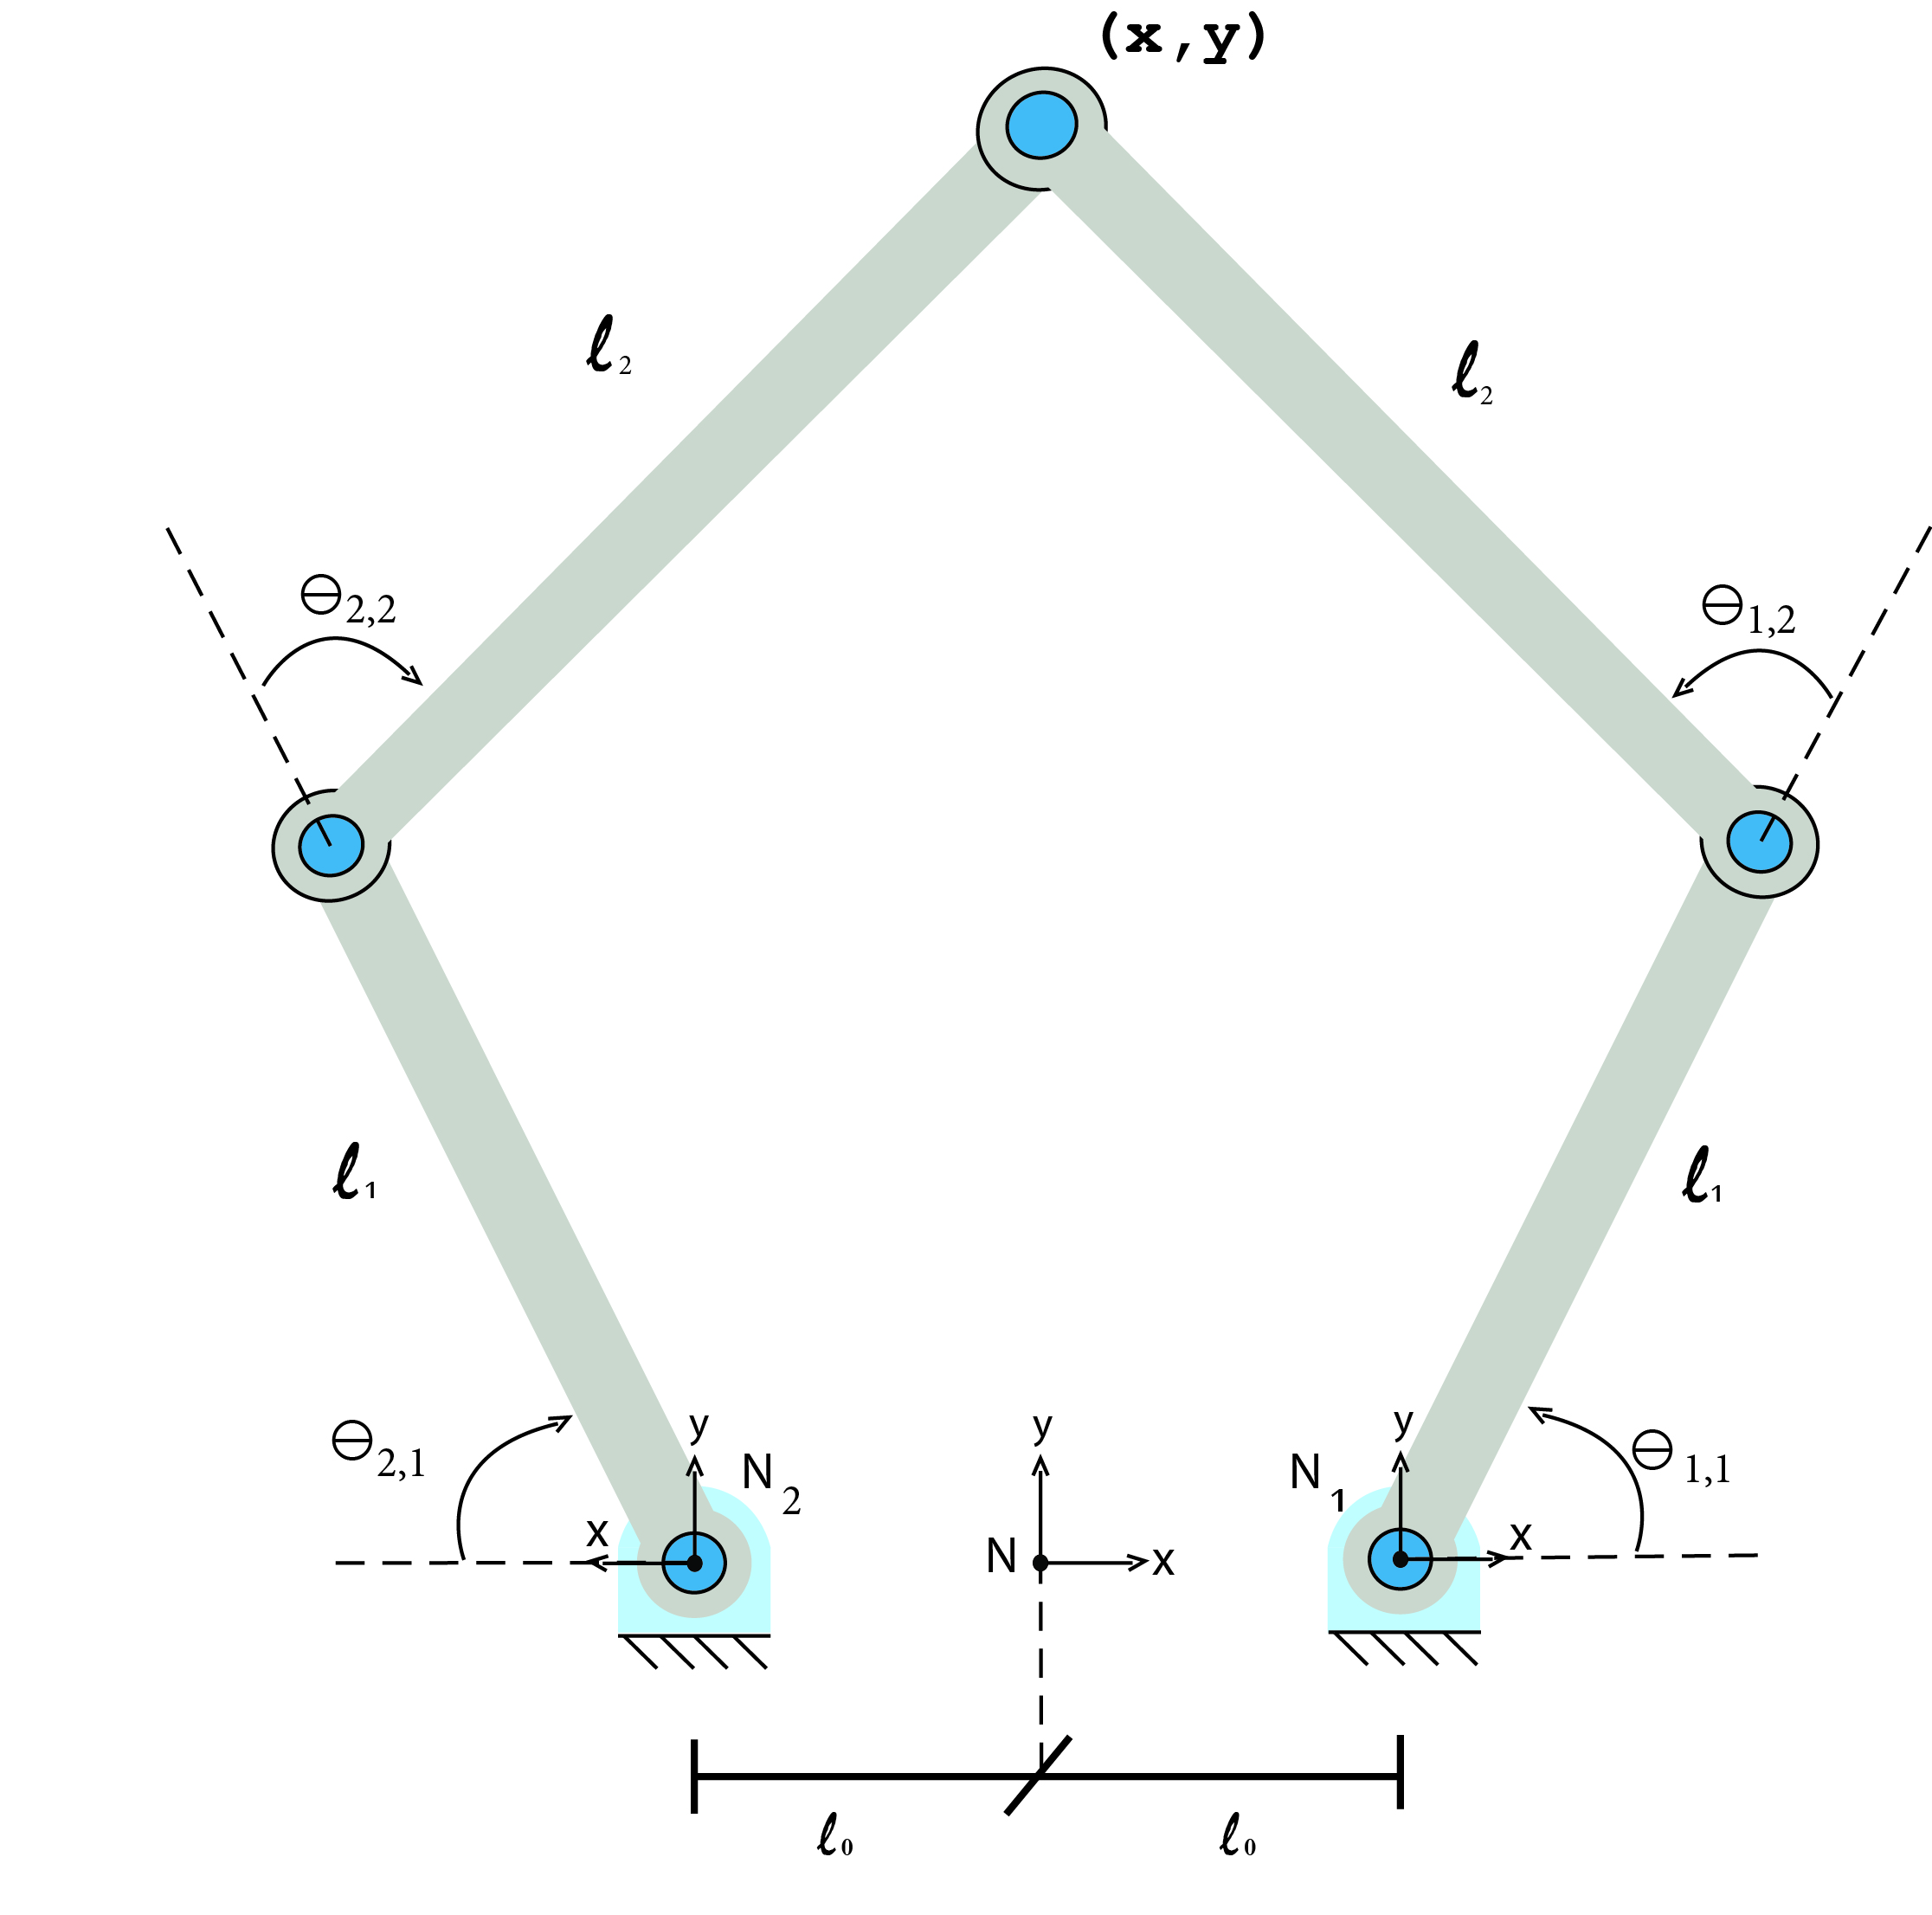
\includegraphics[scale=0.10]{../figures/5Rscan.jpg}  
	\caption{Pentágono articulado (5R)}
	\label{fig:5R}
\end{figure}

O mecanismo 5R será modelado através do acoplamento de 2 subsistemas seriais $\ssB_1$ e $\ssB_2$ do tipo \underline{R}\underline{R}, e um efetuador pontual $\ssB_0$ de massa $m_0$.

\begin{figure}[h]
	\centering
	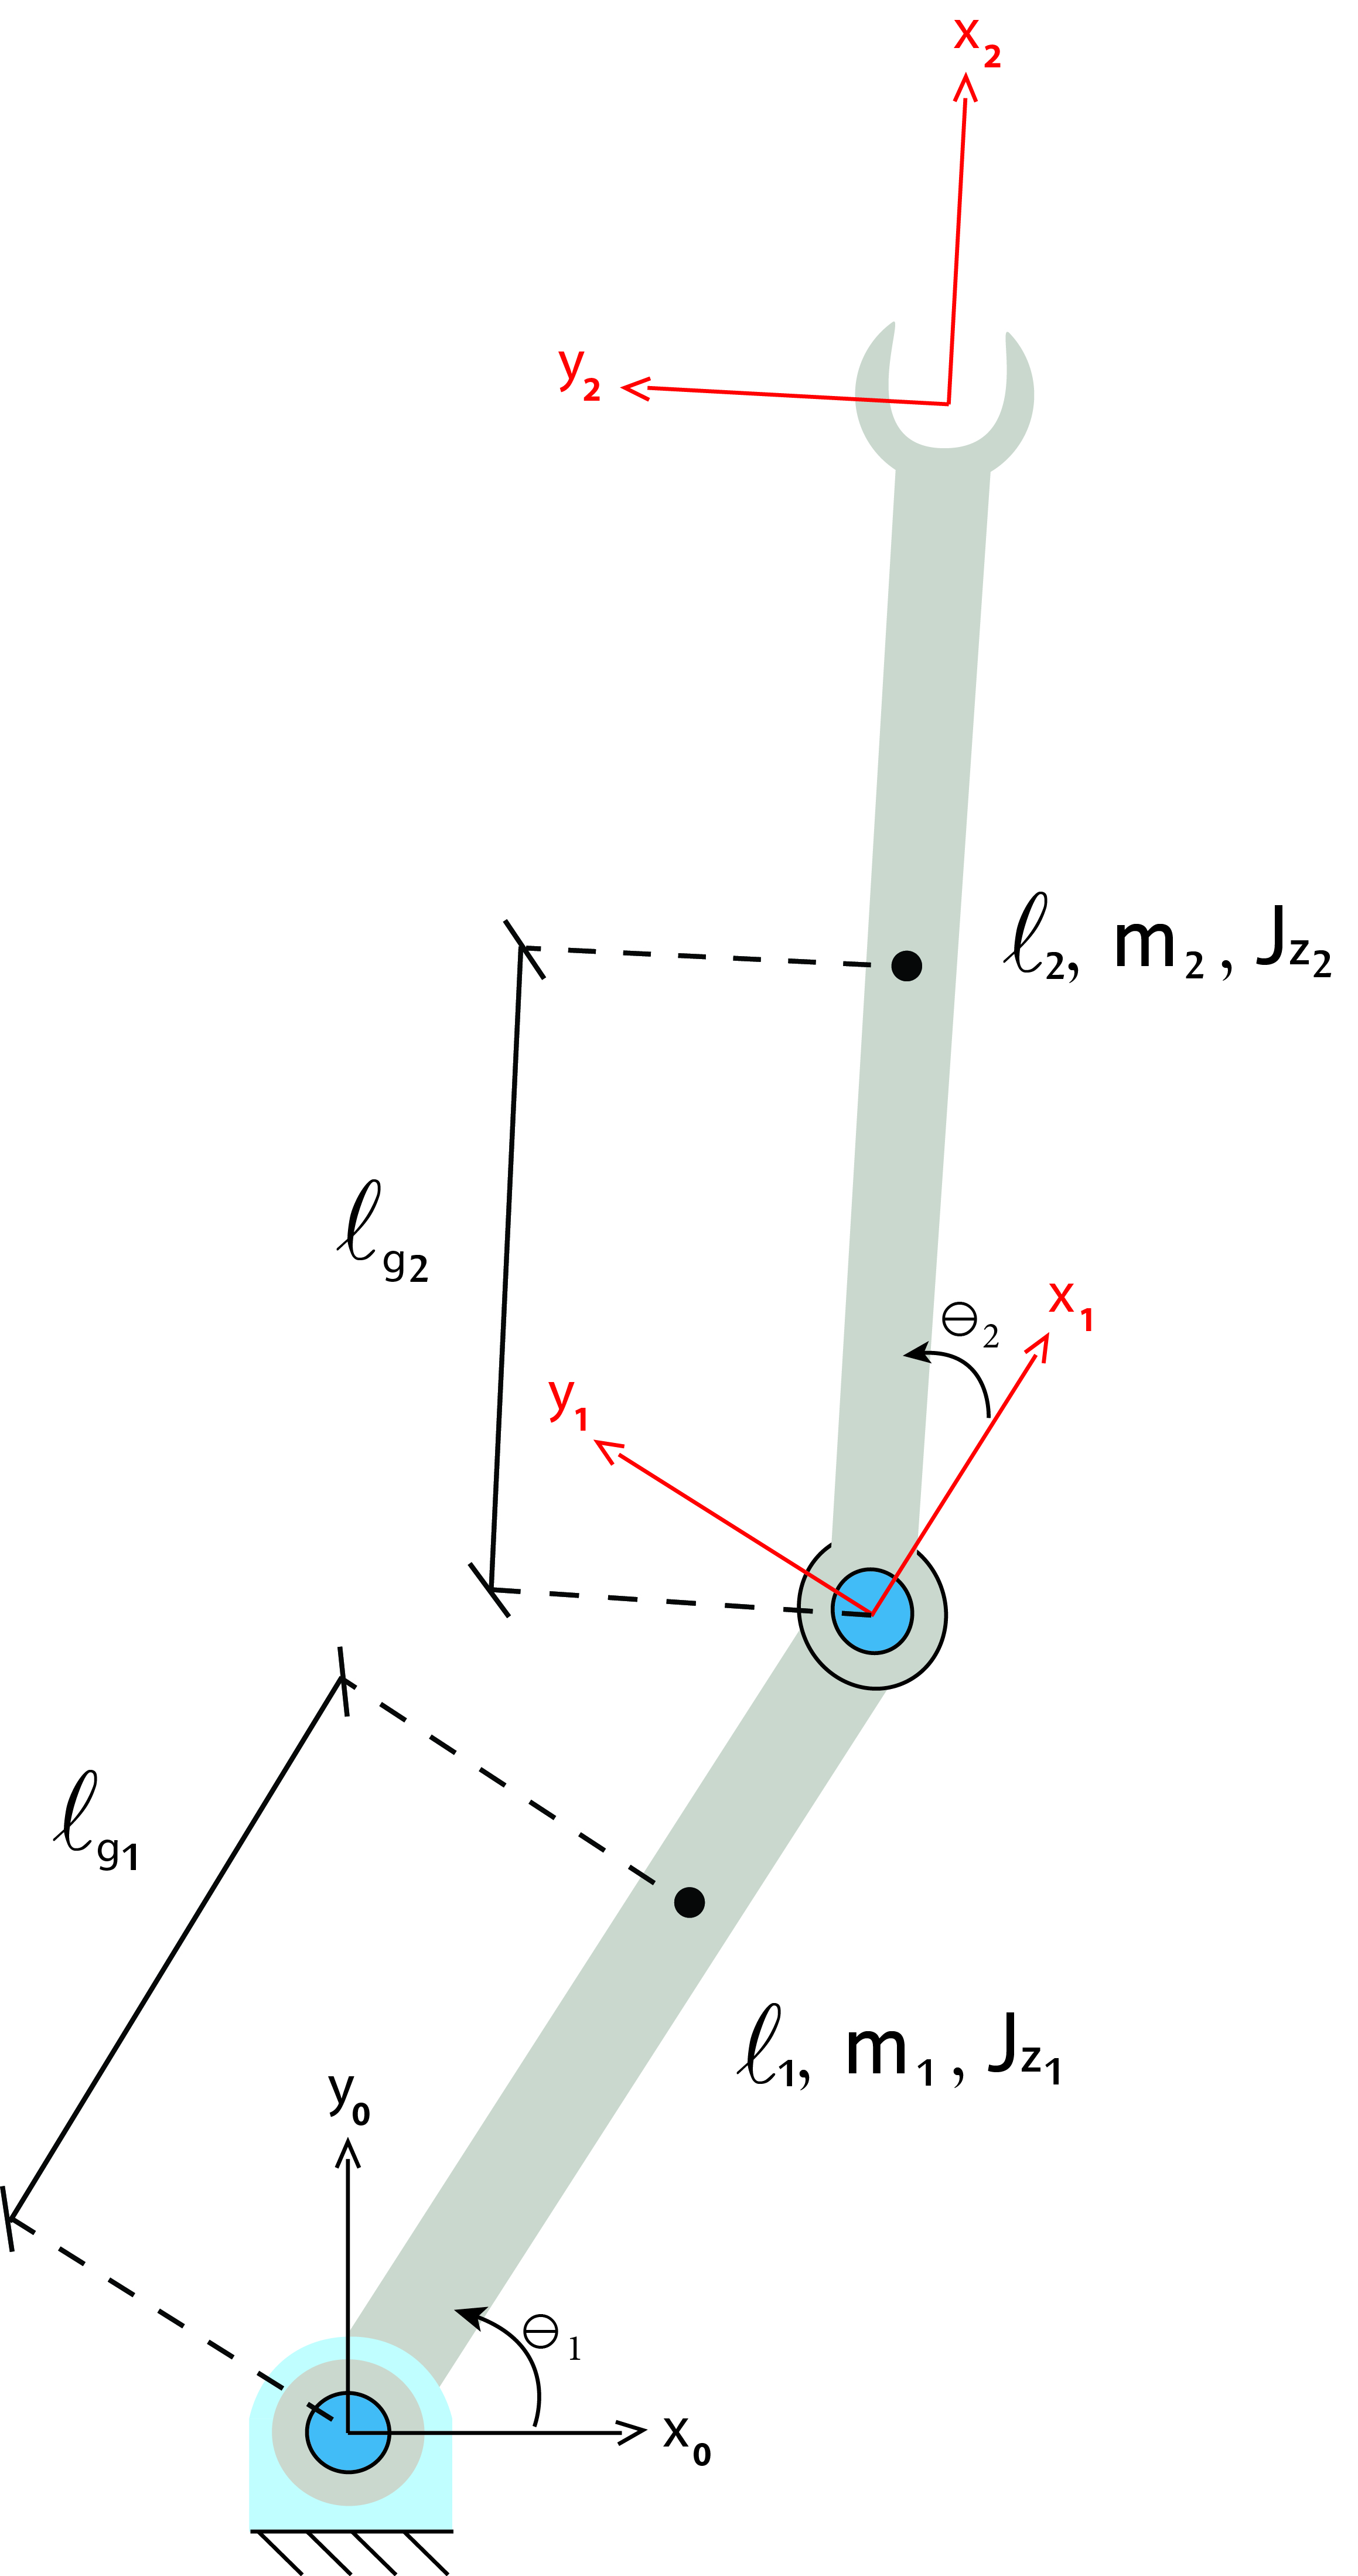
\includegraphics[scale=0.055]{../figures/RR.jpg}  
	\caption{Mecanismo \underline{R}\underline{R}}
	\label{fig:RR}
\end{figure}


\begin{itemize}
\item[i)] Modelo do efetuador

O modelo do efetuador pontual $\ssB_0$ segue o formato dado pela equação \eqref{eq:ModeloDosSubsistemas}, ou seja:
\begin{equation}
\overline{\mf}_{\ssB_0}(\mu_0, \mq_0, \dot{\mq}_0, \ddot{\mq}_0) =  \mu_0 - (\mM_{\ssB_0}(\mq_0) \ddot{\mq}_0 + \mv_{\ssB_0}(\mq_0,\dot{\mq}_0) + \mg_{\ssB_0}(\mq_0)) = \mzr
\end{equation}
Para o subsistema em questão, temos:
\begin{equation}
\mM_{\ssB_0}(\mq_0) = \begin{bmatrix}
m_0 & 0 \\
0 & m_0 \\
\end{bmatrix}
\end{equation}
\begin{equation}
\mv_{\ssB_0}(\mq_0,\dot{\mq}_0) = \mzr
\end{equation}
\begin{equation}
\mg_{\ssB_0}(\mq_0) = \begin{bmatrix}
0 &
m_0 g \\
\end{bmatrix}^\msT
\end{equation}
\begin{equation}
\mq_0 = \mq\ssh = \begin{bmatrix}
x &
y
\end{bmatrix}^\msT
\end{equation}
\begin{equation}
\mu_0 = \mzr
\end{equation}



\item[ii)] Parâmetros de Denavit-Hartemberg das cadeias seriais

\begin{table}[h]
\begin{center}
\caption[DH]{Parâmetros de Denavit-Hartemberg do mecanismo \underline{R}\underline{R}}
\begin{tabular}{|c|c|c|c|c|c|} 
	\hline
	\rule[-2mm]{0mm}{6mm}
	Ligamento & $a_i$ & $\alpha_i$ & $d_i$ & $\theta_i$ \\
	\hline
	\rule[-2mm]{0mm}{6mm}
	(1) & $l_1$ & $0$ & $0$ & $q_1(t)$  \\
	\rule[-1mm]{0mm}{5mm}
	(2) & $l_2$ & $0$ & $0$ & $q_2(t)$  \\
	\hline
\end{tabular}
\label{tab:DH}
\end{center}
\end{table}

\item[iii)] Arquitetura do mecanismo paralelo

É possível relacionar as coordenadas um ponto no espaço descrito no sistema $\ttN$ com as coordenadas do mesmo ponto escritas nos sistemas $\ttN_1$ e $\ttN_2$ da seguinte maneira:
\begin{equation}
\vct{\ttp}_{\ttN} = \begin{bmatrix}
1 & 0 & 0 \\
0 & 1 & 0 \\
0 & 0 & 1 \\
\end{bmatrix}
\cdot
\vct{\ttp}_{\ttN_1}
+
\begin{bmatrix}
l_0 \\
0 \\
0 
\end{bmatrix}
\end{equation}
\begin{equation}
\vct{\ttp}_{\ttN} = \begin{bmatrix}
-1 & 0 & 0 \\
0 & 1 & 0 \\
0 & 0 & -1 \\
\end{bmatrix}
\cdot
\vct{\ttp}_{\ttN_2}
+
\begin{bmatrix}
-l_0 \\
0 \\
0 
\end{bmatrix}
\end{equation}

Escolhendo o ponto $\ttp$ como sendo o efetuador do mecanismo paralelo, o qual tem a mesma localização dos efetuadores das cadeias serias neste caso, temos:
\begin{equation}
\mq\ssh = 
\begin{bmatrix}
1 & 0 & 0 \\
0 & 1 & 0 \\
\end{bmatrix}
\cdot
\mx_1(\mq_1)
+
\begin{bmatrix}
l_0 \\
0 \\
\end{bmatrix}
\end{equation}
\begin{equation}
\mq\ssh = 
\begin{bmatrix}
-1 & 0 & 0 \\
0 & 1 & 0 \\
\end{bmatrix}
\cdot
\mx_2(\mq_2)
+
\begin{bmatrix}
-l_0 \\
0 \\
\end{bmatrix}
\end{equation}

Sendo assim, temos que os vínculos de posição são dados por:
\begin{equation}
\overline{\mq}(\mq) =
\begin{bmatrix}
1 & 0 \\
0 & 1 \\
1 & 0 \\
0 & 1 \\
\end{bmatrix}
\cdot
\mq\ssh
-
\begin{bmatrix}
1 & 0 & 0 & 0 & 0 & 0 \\
0 & 1 & 0 & 0 & 0 & 0 \\
0 & 0 & 0 & -1 & 0 & 0 \\
0 & 0 & 0 & 0 & 1 & 0 \\
\end{bmatrix}
\cdot
\mx(\mq\cir)
-
\begin{bmatrix}
l_0 \\
0 \\
-l_0 \\
0 \\
\end{bmatrix}
= \mzr
\end{equation}

Como não temos vínculos de velocidades angulares para esse mecanismo, as matrizes que descrevem a arquitetura do mecanismo são dadas por:
\begin{multicols}{3}
\begin{equation}
\md = \begin{bmatrix}
l_0 \\
0 \\
-l_0 \\
0 \\
\end{bmatrix}
\end{equation} \\
\begin{equation}
\mD = \begin{bmatrix}
1 & 0 \\
0 & 1 \\
1 & 0 \\
0 & 1 \\
\end{bmatrix}
\end{equation} \\
\begin{equation}
\mE = \begin{bmatrix}
1 & 0 & 0 & 0 & 0 & 0 \\
0 & 1 & 0 & 0 & 0 & 0 \\
0 & 0 & 0 & -1 & 0 & 0 \\
0 & 0 & 0 & 0 & 1 & 0 \\
\end{bmatrix}
\end{equation}
\end{multicols}
\begin{equation}
\mF = \mzr
\end{equation}
\begin{equation}
\mP = \mQ = \mR = \vct{\varnothing}
\end{equation}

\item[iv)] Parâmetros e incertezas do modelo

Definimos os seguinte parâmetros e incertezas para o mecanismo em questão:

\begin{multicols}{2}
\begin{itemize}
\item[-] $l_1 = 0.12 m$
\item[-] $l_2 = 0.15 m$
\item[-] $l_{g1} = (0.06 \pm 0.009) m$
\item[-] $l_{g2} = (0.075 \pm 0.011) m$
\item[-] $m_0 = 0 \, kg$
\item[-] $m_1 = (0.143 \pm 0.0215) kg$
\item[-] $m_2 = (0.171 \pm 0.0257) kg$
\item[-] $Jz_1 = (171.6 \pm 25.7 ) 10^{-6} kg\cdot m^2$
\item[-] $Jz_2 = (320.6 \pm 48.1 ) 10^{-6} kg\cdot m^2$
\item[-] $g = 9.8 m/s^2$
\end{itemize}
\end{multicols}

\item[v)] Espaço de trabalho

Dados os parâmetros geométricos defidos acima, obtemos o seguinte espaço de trabalho para o mecanismo:

\begin{figure}[h]
	\centering
	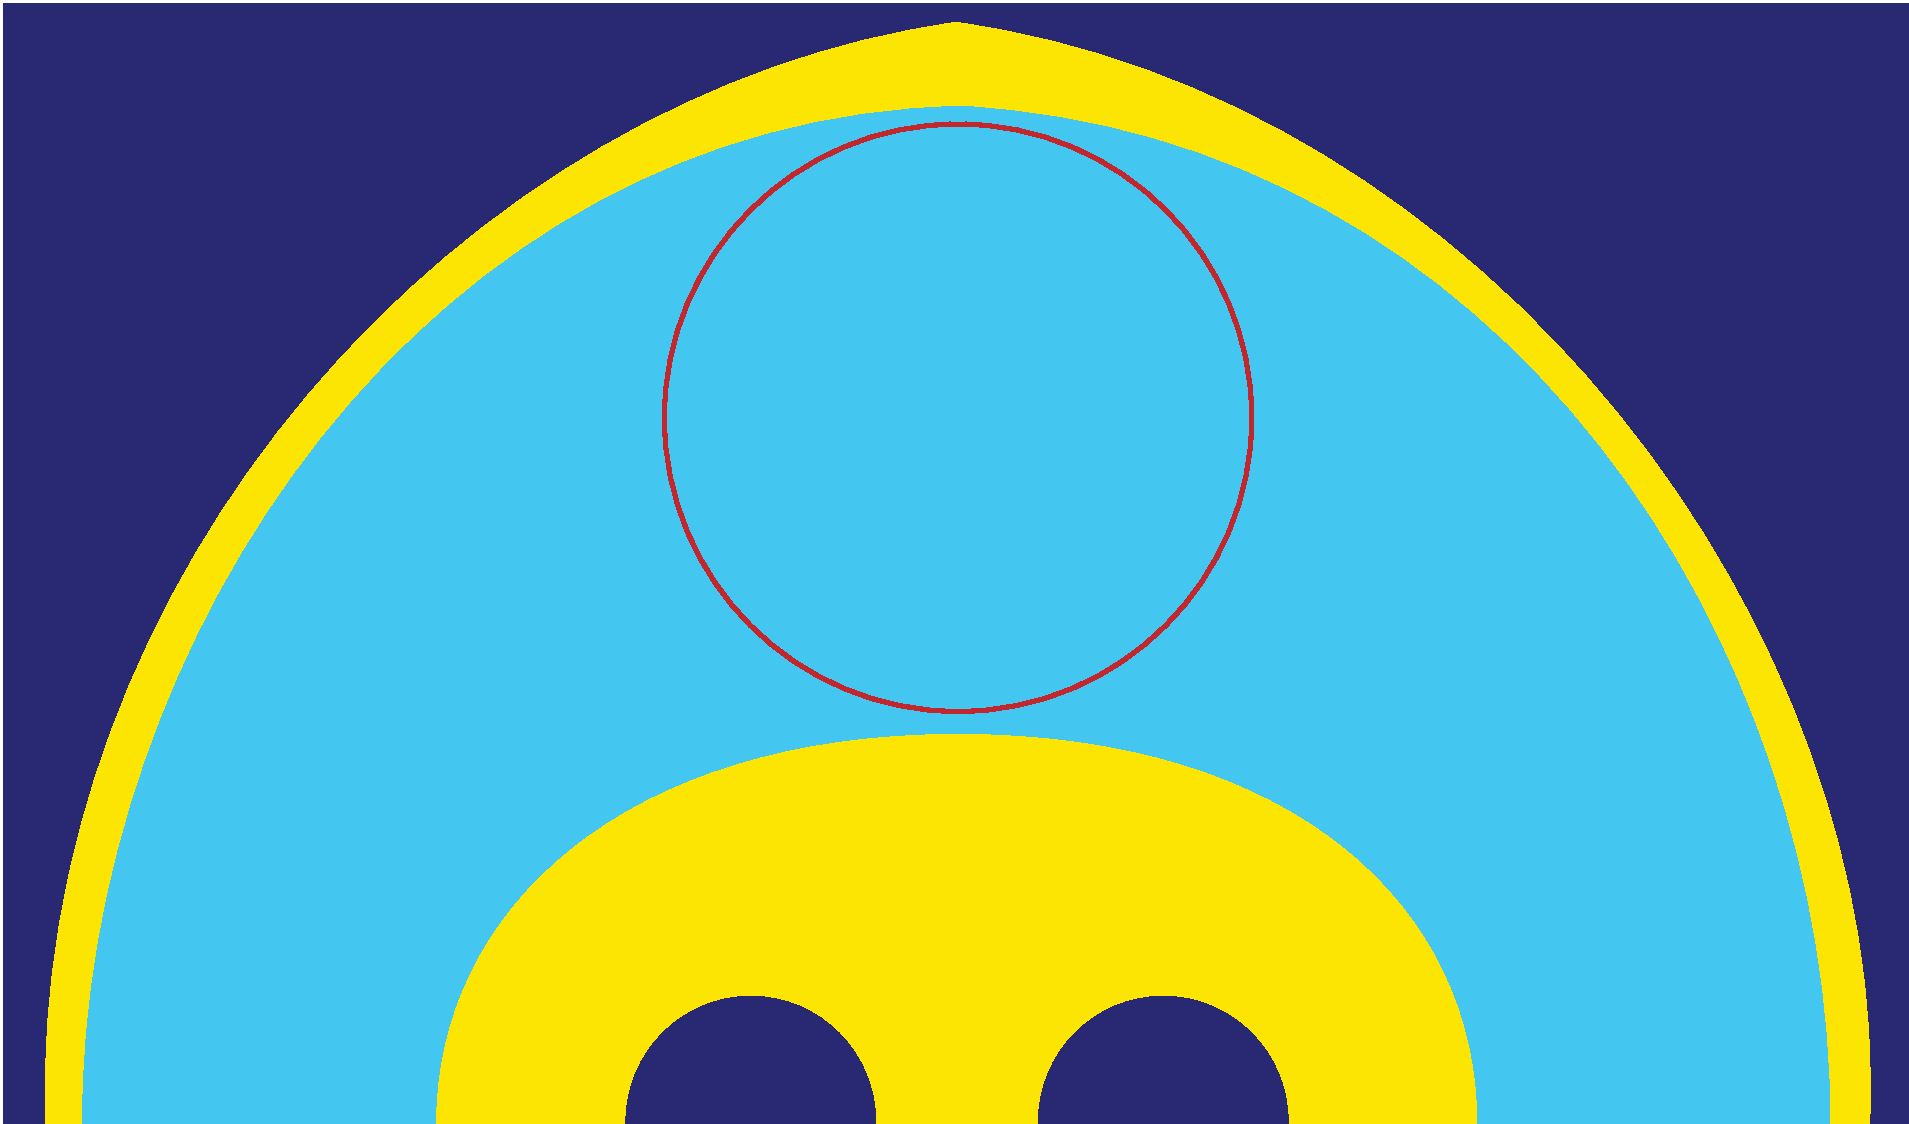
\includegraphics[scale=0.25]{../figures/Workspace.pdf}  
	\caption{Espaço de trabalho do mecanismo 5R}
	\label{fig:RRWS}
\end{figure}

A região em azul escuro é a região não pertencente ao espaço de trabalho do mecanismo. As regiões em azul claro, em amarelo, e em vermelho são regiões pertencententes ao espaço do mecanismo. A região a amarela é considerada singular (próxima a singularidades) e a vermelha é a trajetória a ser seguida pelo mecanismo.

\item[vi)] Controlador

A lei de controle por modos deslizantes que será utilizada na simulação dinâmica direta é dada pelas equações \eqref{eq:ControlLawSRed} e \eqref{eq:MatriDiagk2}. $\mGamma$, $\meta$ e $\meta_{i,j}$ são obtidas da seguinte maneira:
\begin{itemize}
\item[$\bullet$] Discretiza-se o espaço de trabalho em um número finito de pontos considerados não-singulares. Foi adotada um discretização de $1 cm$ na horizontal e na vertical.
\item[$\bullet$] Para cada ponto calcula-se $|\mDelta|$, $|\mdelta_0|$ e $|\mdelta_{i,j}|$ para todas as combinações possíveis de parâmetros, com os parâmetros podendo assumir seu valor mínimo e seu valor máximo. Como temos 6 parâmetros incertos, temos 64 possibilidades.
\item[$\bullet$] Obtem-se o valor máximo de $|\mDelta|$, $|\mdelta_0|$ e $|\mdelta_{i,j}|$ para cada ponto.
\item[$\bullet$] Obtem-se o valor máximo de $|\mDelta|$, $|\mdelta_0|$ e $|\mdelta_{i,j}|$ para o espaço de trabalho, a partir do valor máximo em cada ponto.
\end{itemize}

Realizando-se esse procedimento e adotando $\eta = 20.0$, obtemos:
\begin{equation}
\diag(\underline{k}) =
\begin{bmatrix}
75.3 \\
108
\end{bmatrix}
+
\begin{bmatrix}
37.0 \\
54.1
\end{bmatrix} \dot{x}^2
+
\begin{bmatrix}
22.7 \\
35.5
\end{bmatrix} |\dot{x} \dot{y} |
+
\begin{bmatrix}
17.5 \\
28.5
\end{bmatrix} \dot{y}^2
+
\begin{bmatrix}
1.25 & 0.92 \\
1.68 & 1.65
\end{bmatrix}
\cdot
\begin{bmatrix}
|\ddot{x}_d + \lambda \dot{e}_x| \\
|\ddot{y}_d + \lambda \dot{e}_y|
\end{bmatrix}
\end{equation}

\item[vi)] Simulação dinâmica direta

Para realizar a simulação dinâmica direta, definimos:

\begin{itemize}

\item[$\bullet$] Parâmetros do mecanismo:
\begin{multicols}{2}
\begin{itemize}
\item[-] $l_1 = 0.12 m$
\item[-] $l_2 = 0.15 m$
\item[-] $l_{g1} = 0.051 m$
\item[-] $l_{g2} = 0.086 m$
\item[-] $m_0 = 0 \, kg$
\item[-] $m_1 = 0.1645 kg$
\item[-] $m_2 = 0.1967 kg$
\item[-] $Jz_1 = 197.3 \cdot 10^{-6} kg\cdot m^2$
\item[-] $Jz_2 = 368.7 \cdot 10^{-6} kg\cdot m^2$
\item[-] $g = 9.8 m/s^2$
\end{itemize}
\end{multicols}

\item[$\bullet$] Parâmetros estimados
\begin{multicols}{2}
\begin{itemize}
\item[-] $\hat{l}_1 = 0.12 m$
\item[-] $\hat{l}_2 = 0.15 m$
\item[-] $\hat{l}_{g1} = 0.06 m$
\item[-] $\hat{l}_{g2} = 0.075 m$
\item[-] $\hat{m}_0 = 0 \, kg$
\item[-] $\hat{m}_1 = 0.143 kg$
\item[-] $\hat{m}_2 = 0.171 kg$
\item[-] $\hat{J}z_1 = 171.6 \cdot 10^{-6} kg\cdot m^2$
\item[-] $\hat{J}z_2 = 320.6 \cdot 10^{-6} kg\cdot m^2$
\item[-] $\hat{g} = 9.8 m/s^2$
\end{itemize}
\end{multicols}

\item[$\bullet$] Condições iniciais:
\begin{equation}
\begin{cases}
q\ssh_1(0) = 0.07 m\\
q\ssh_2(0) = 0.17 m \\
\dot{q}\ssh_1(0) = 0 \\
\dot{q}\ssh_2(0) = 0 \\
\end{cases}
\end{equation}

\item[$\bullet$] Trajetória de referência:
\begin{equation}
\begin{cases}
q\ssh_{1 \, d}(t) = 0.07 \cos(28.57 t) \\
q\ssh_{2 \, d}(t) = 0.17 + 0.07 \sin(28.57 t) \\
\end{cases}
\end{equation}

\item[$\bullet$] Parâmetros do controlador:
$$ \lambda = 40.0 $$
$$ \eta = 20.0 $$

Os parâmetros do mecanismo foram escolhidos de modo que haja um erro de $15\%$ em cada parâmetro incerto.
Os parâmetros do controlador foram escolhidos de modo que o sistema tenha um tempo de alcance às superfícies de escorregamento $t_r  \leq 0.1 s$ (pois $\ms(0) = [0 \; -2]^\msT$) e um tempo de assentamento de $t_a = 0.1 s$, quando o sistema chega nas superfícies de escorregamento. \\
\end{itemize}

A função $f(x) = \sign(x)$ foi substituida pela função de saturação $f_{sat}(x) = \tanh(100 x)$, a qual tem as seguintes propriedades:
\begin{itemize}
\item[-] $f_{sat}(0.023) = -f_{sat}(-0.023) = 0.98$
\item[-] $f_{sat}(\infty) = -f_{sat}(-\infty) = 1$
\item[-] $ \frac{\dd f_{sat}}{\dd x} (0) = 100$
\end{itemize}

Sua utilização garante a estabilidade nas simulações numéricas, evita o chattering nos atuadores, e ainda garante um erro em regime permanente desprezível para esta aplicação.

\begin{figure}[h]
	\centering
	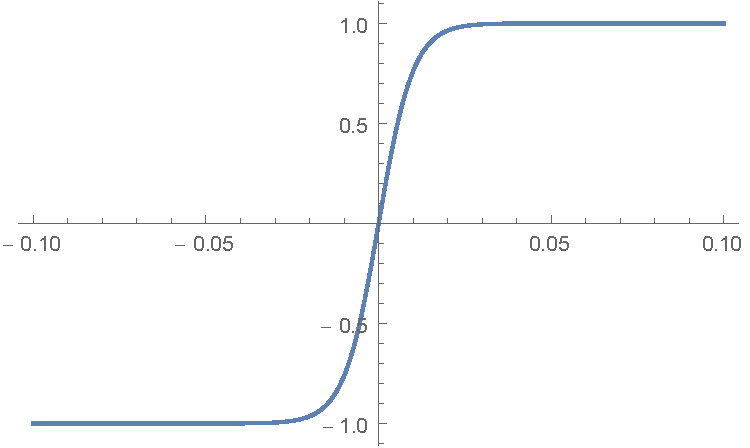
\includegraphics[scale=0.4]{../figures/Tanh.pdf}  
	\caption{Função de saturação $f_{sat}(x) = \tanh(100 x)$}
	\label{fig:Tanh}
\end{figure}

\end{itemize}

Aqui seguem os resultados das simulações numéricas:

\newpage

\begin{multicols}{2}
\begin{figure}[H]
	\centering
	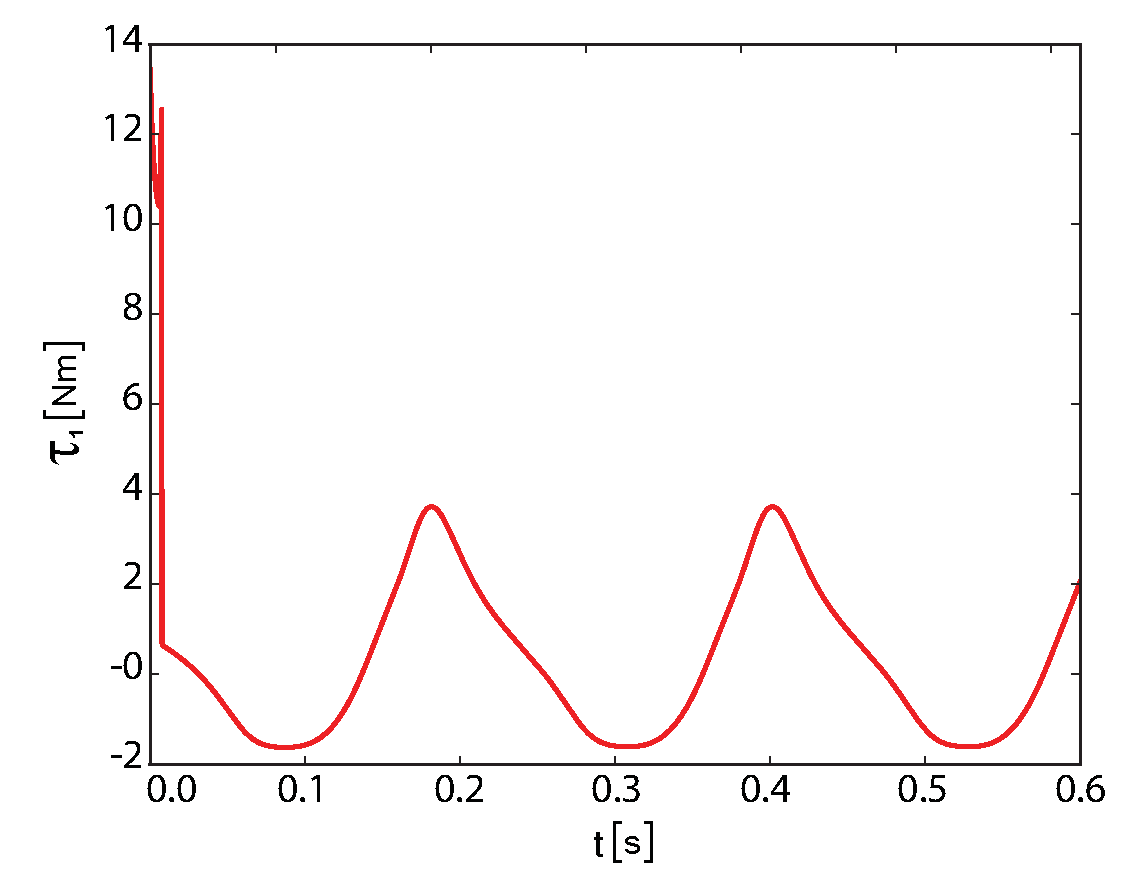
\includegraphics[scale=0.31]{../figures/Torque1.pdf}  
	\caption{Torque aplicado pelo atuador 1}
	\label{fig:Torque1}
\end{figure}

\begin{figure}[H]
	\centering
	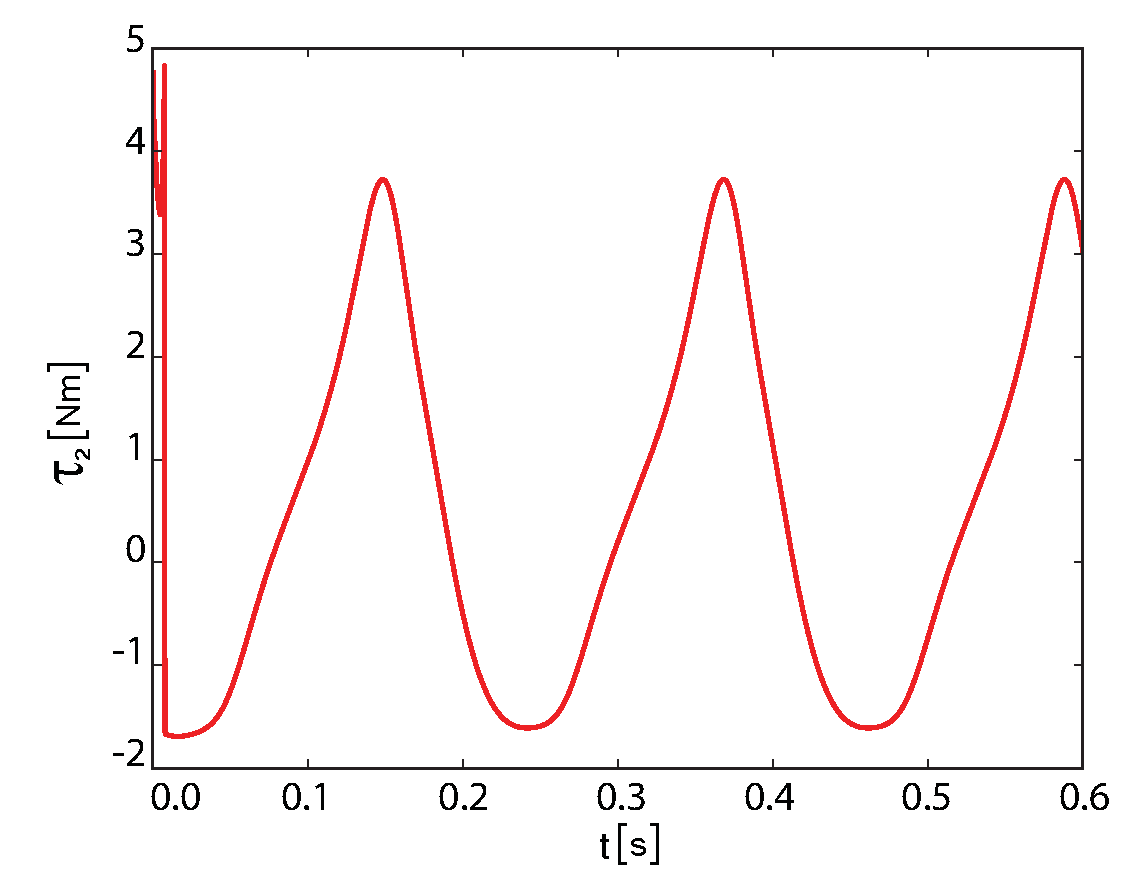
\includegraphics[scale=0.31]{../figures/Torque2.pdf}  
	\caption{Torque aplicado pelo atuador 2}
	\label{fig:Torque2}
\end{figure}
\end{multicols}
\begin{multicols}{2}
\begin{figure}[H]
	\centering
	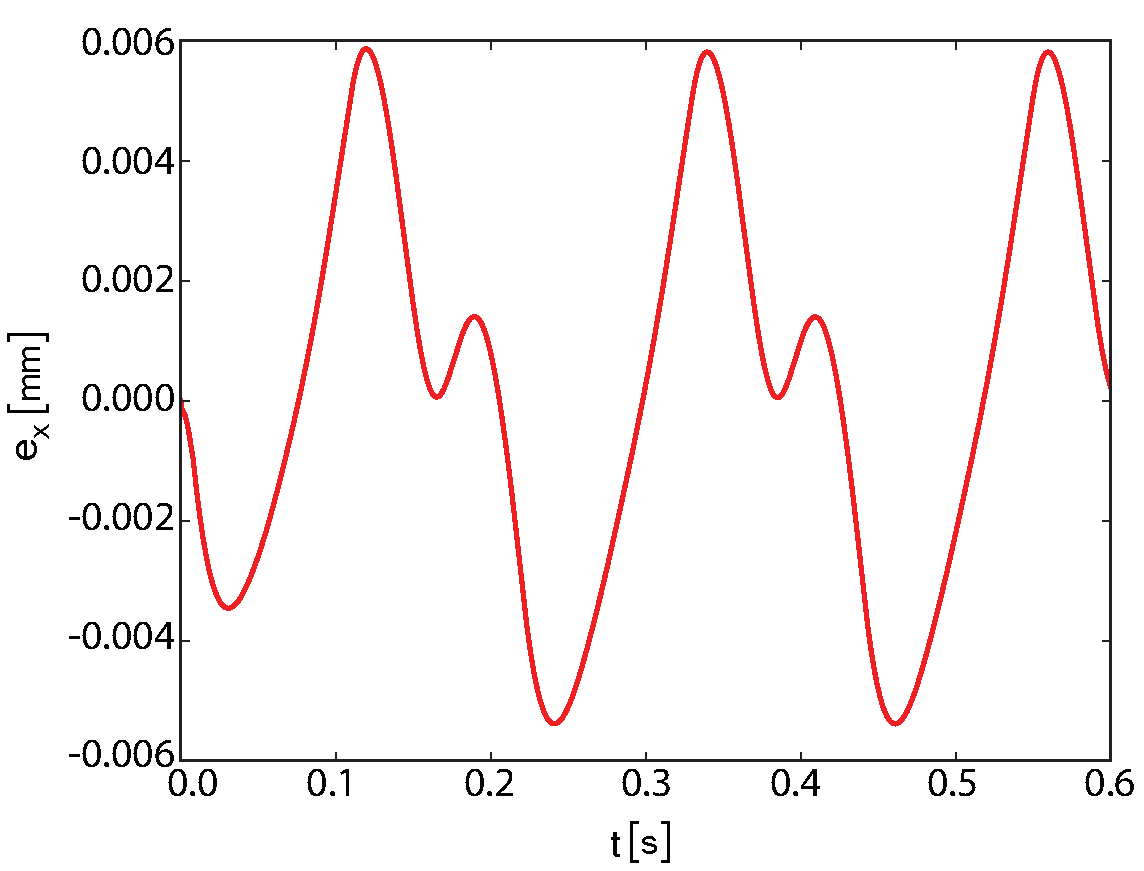
\includegraphics[scale=0.31]{../figures/ex.pdf}  
	\caption{Erro de na coordenada $x$}
	\label{fig:ex}
\end{figure}

\begin{figure}[H]
	\centering
	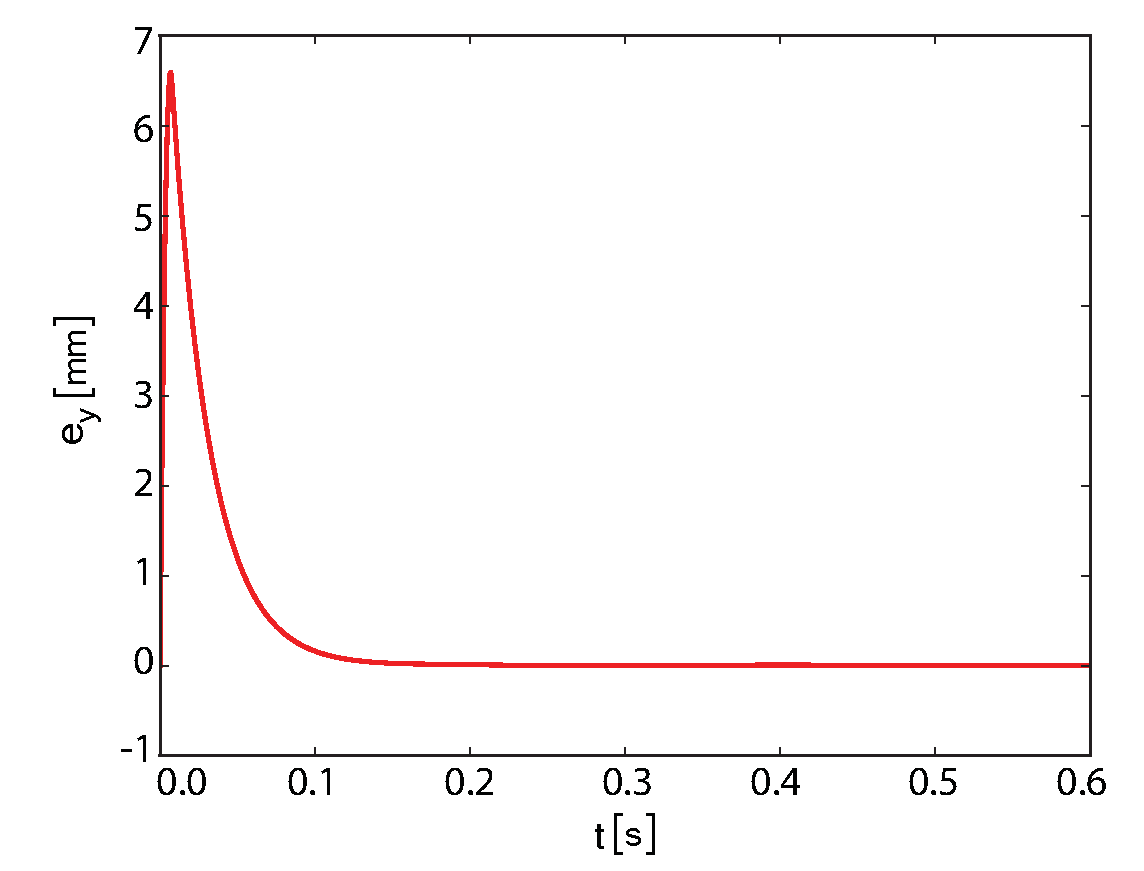
\includegraphics[scale=0.31]{../figures/ey.pdf}  
	\caption{Erro de na coordenada $y$}
	\label{fig:ey}
\end{figure}
\end{multicols}
\begin{multicols}{2}
\begin{figure}[H]
	\centering
	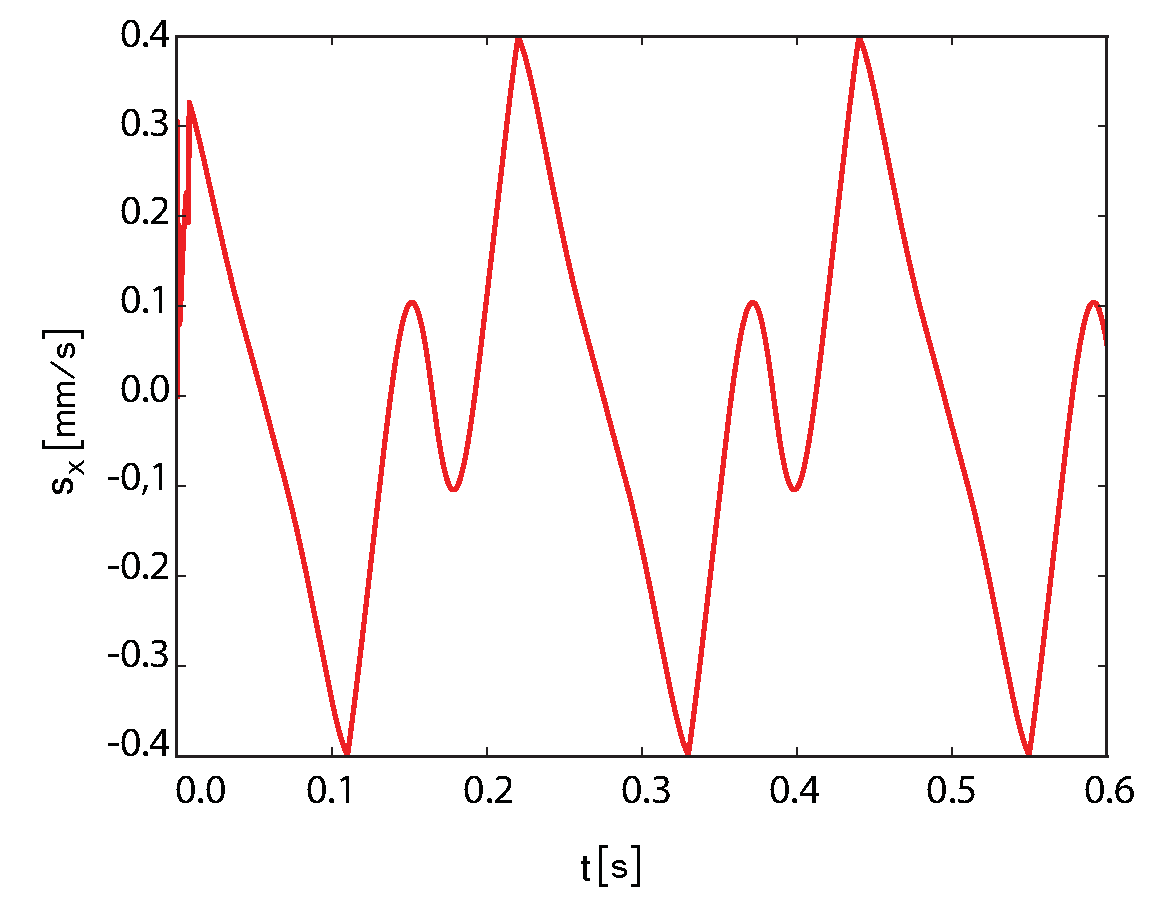
\includegraphics[scale=0.31]{../figures/sx.pdf}  
	\caption{Variável $s_x$}
	\label{fig:sx}
\end{figure}

\begin{figure}[H]
	\centering
	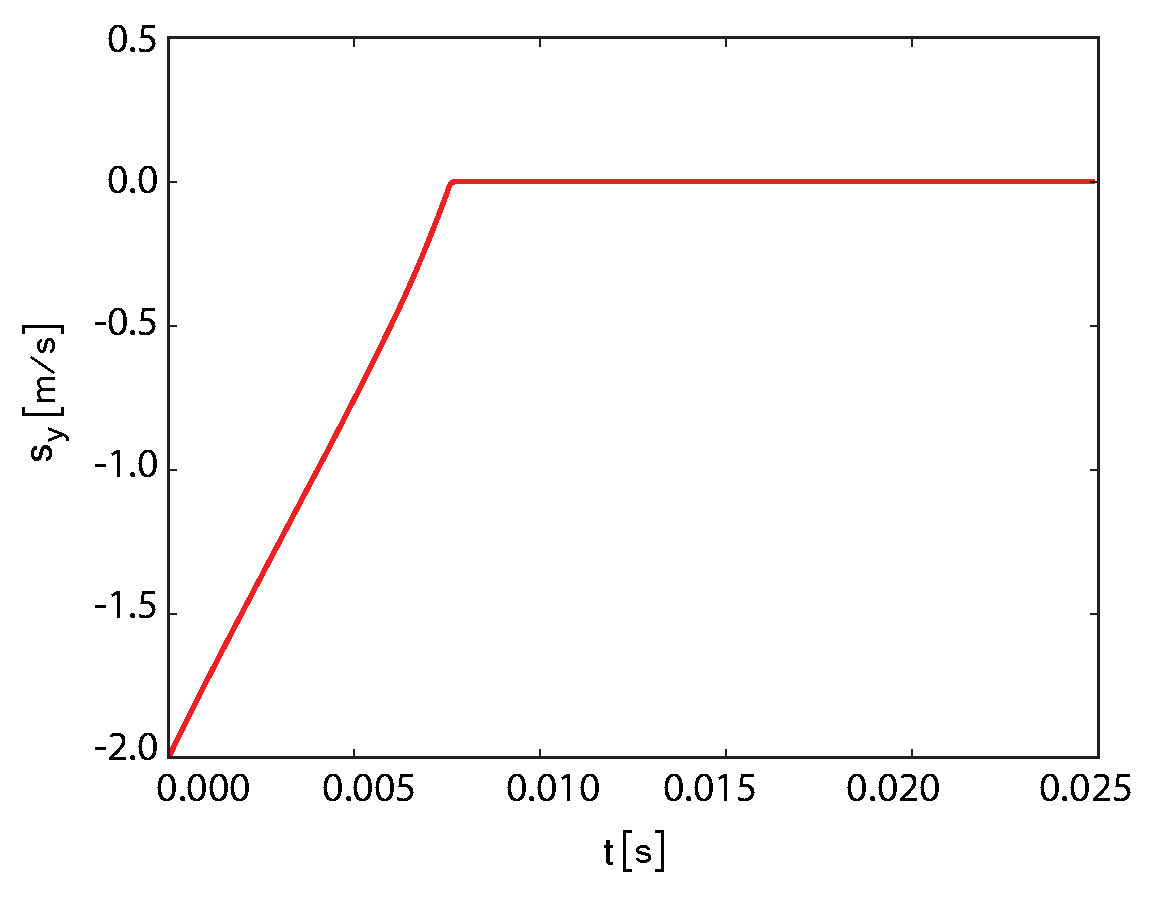
\includegraphics[scale=0.31]{../figures/sy.pdf}  
	\caption{Variável $s_y$}
	\label{fig:sy}
\end{figure}
\end{multicols}

Repare que o tempo de alcance de $s_y$ é aproximadamente $t_r = 0.008s < 0.1s$. Além disso, $0.1s$ depois de alcançar a superfície de escorregamento, o erro $e_y$ já é praticamente nulo, como pode-se observar no gráfico da figura \ref{fig:ey}. Sendo assim, temos os resultados coerentes com os parâmetros do controlador adotados. \\

O projeto do controlador foi feito supondo incertezas de $15\%$ nos parâmetros incertos. Porém, realizando a simulação com o mesmo controlador, aumentando para $50\%$ os erros paramétricos, pode-se observar que o sistema ainda consegue ser controlado, com erros de controle na ordem de centésimos de milímetro, como pode ser visto nos resultados abaixo: 

\begin{multicols}{2}
\begin{figure}[H]
	\centering
	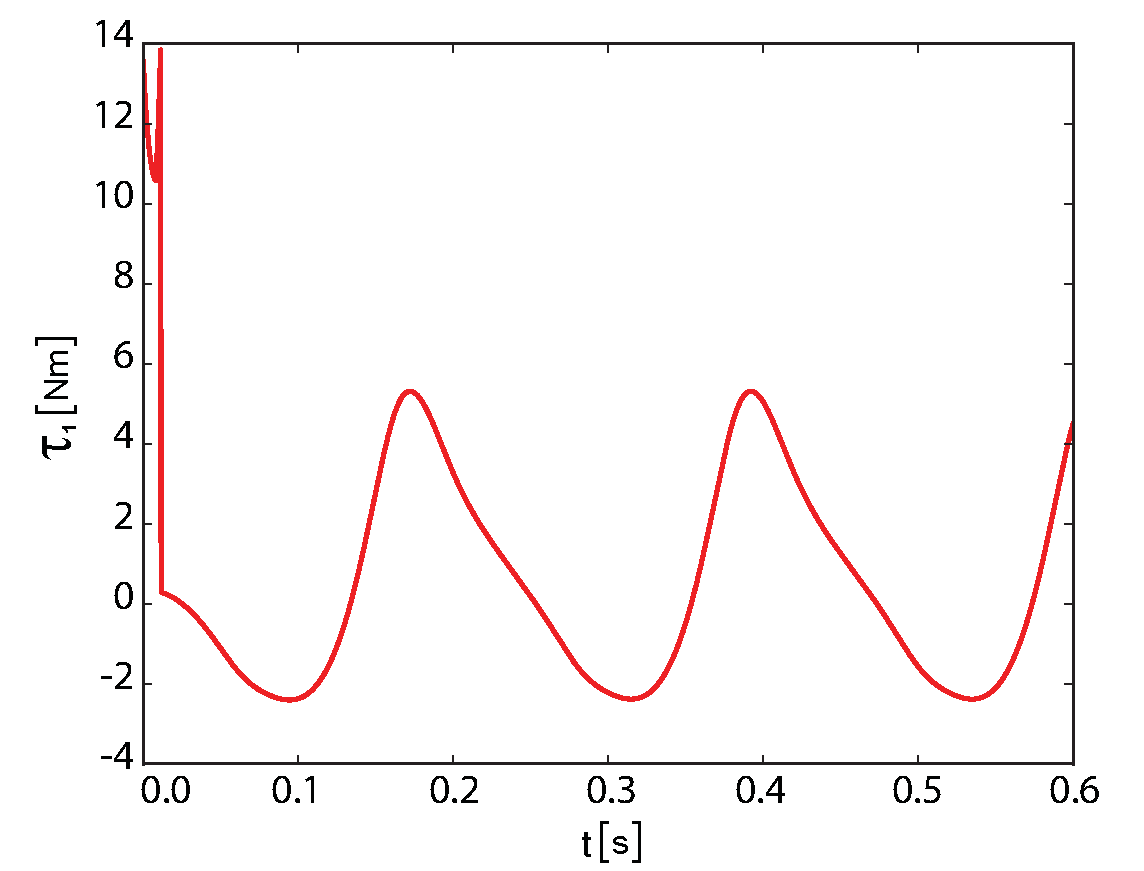
\includegraphics[scale=0.31]{../figures/Torque12.pdf}  
	\caption{Torque aplicado pelo atuador 1}
	\label{fig:Torque12}
\end{figure}

\begin{figure}[H]
	\centering
	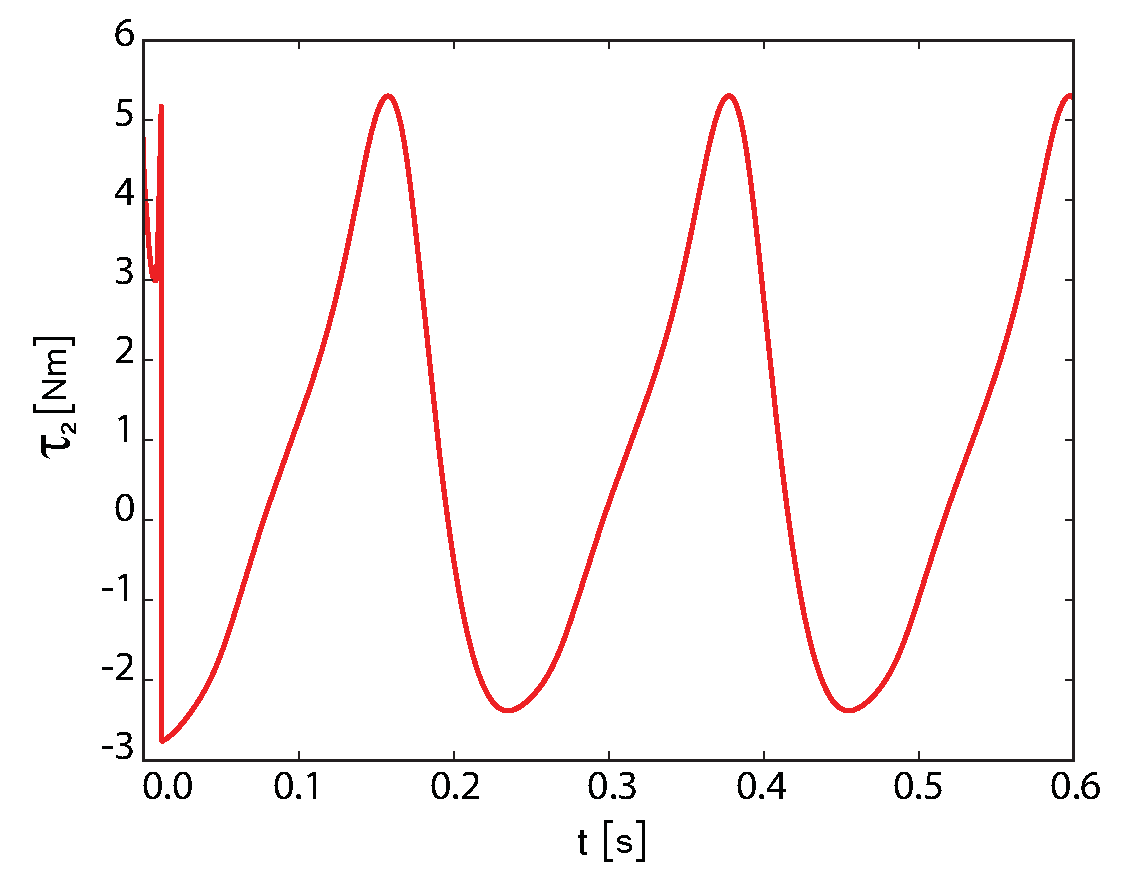
\includegraphics[scale=0.31]{../figures/Torque22.pdf}  
	\caption{Torque aplicado pelo atuador 2}
	\label{fig:Torque22}
\end{figure}
\end{multicols}
\begin{multicols}{2}
\begin{figure}[H]
	\centering
	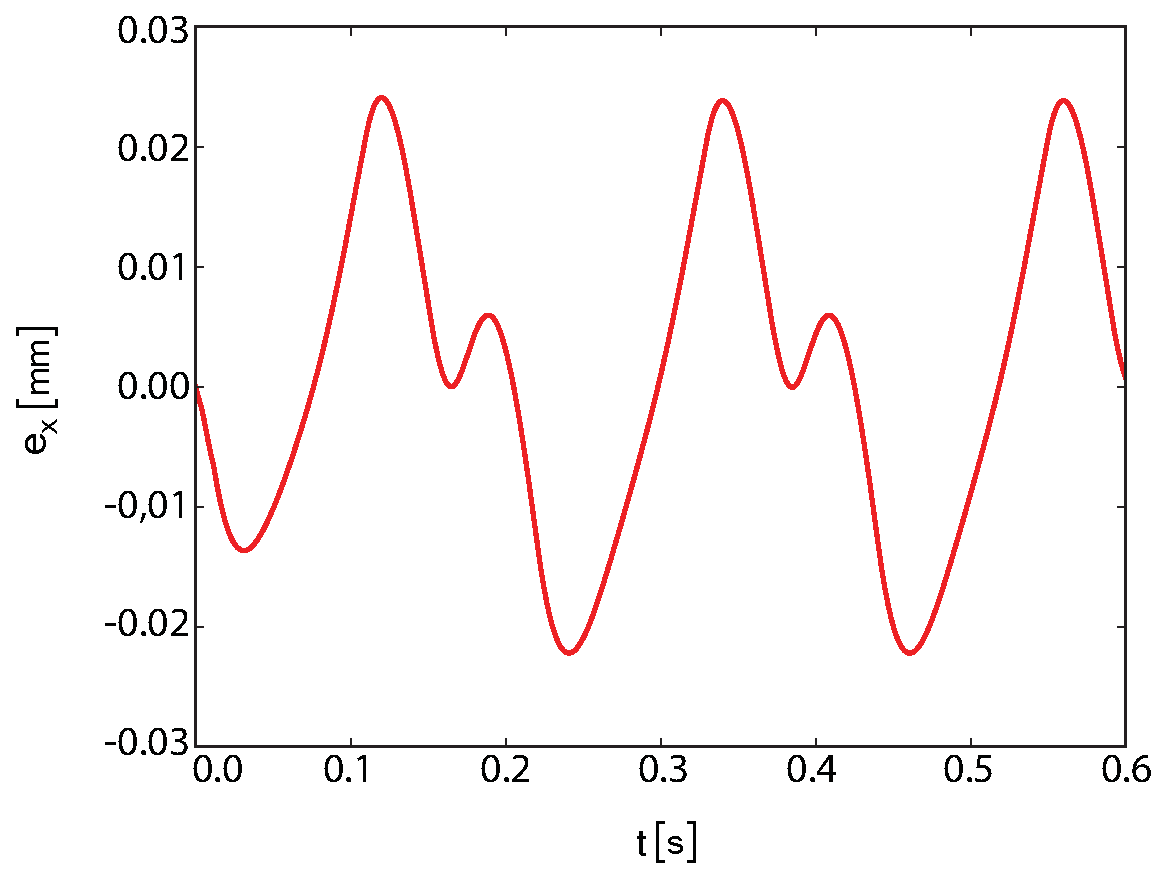
\includegraphics[scale=0.31]{../figures/ex2.pdf}  
	\caption{Erro de na coordenada $x$}
	\label{fig:ex2}
\end{figure}

\begin{figure}[H]
	\centering
	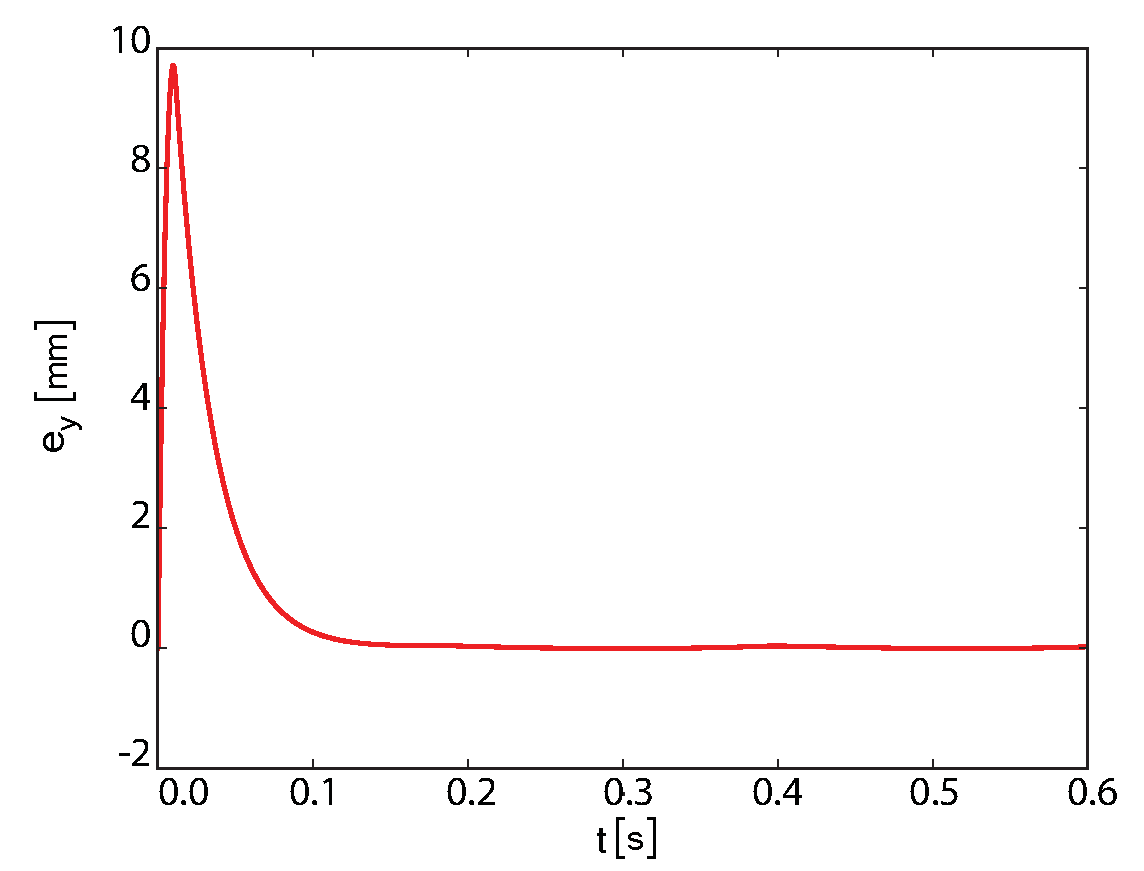
\includegraphics[scale=0.31]{../figures/ey2.pdf}  
	\caption{Erro de na coordenada $x$}
	\label{fig:ey2}
\end{figure}
\end{multicols}

\begin{multicols}{2}
\begin{figure}[H]
	\centering
	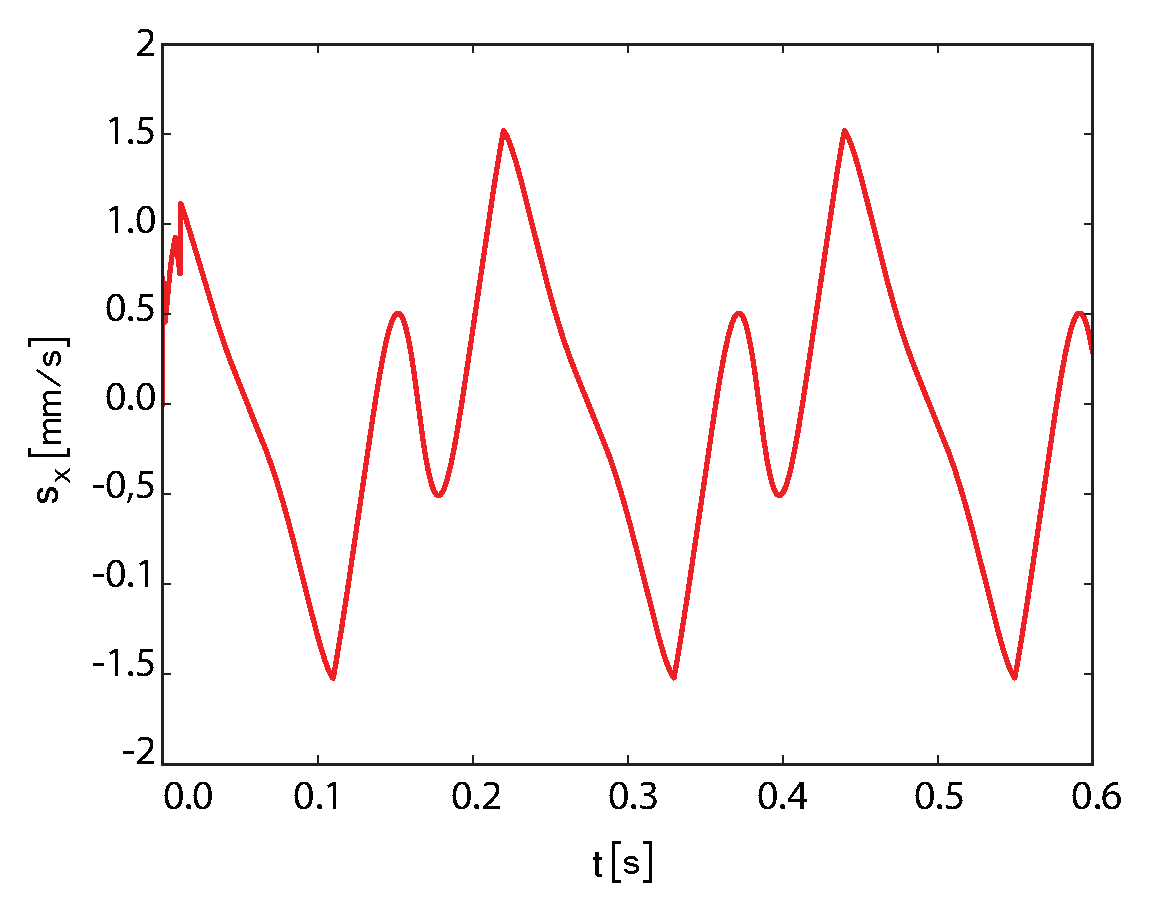
\includegraphics[scale=0.31]{../figures/sx2.pdf}  
	\caption{Variável $s_x$}
	\label{fig:sx2}
\end{figure}
\begin{figure}[H]
	\centering
	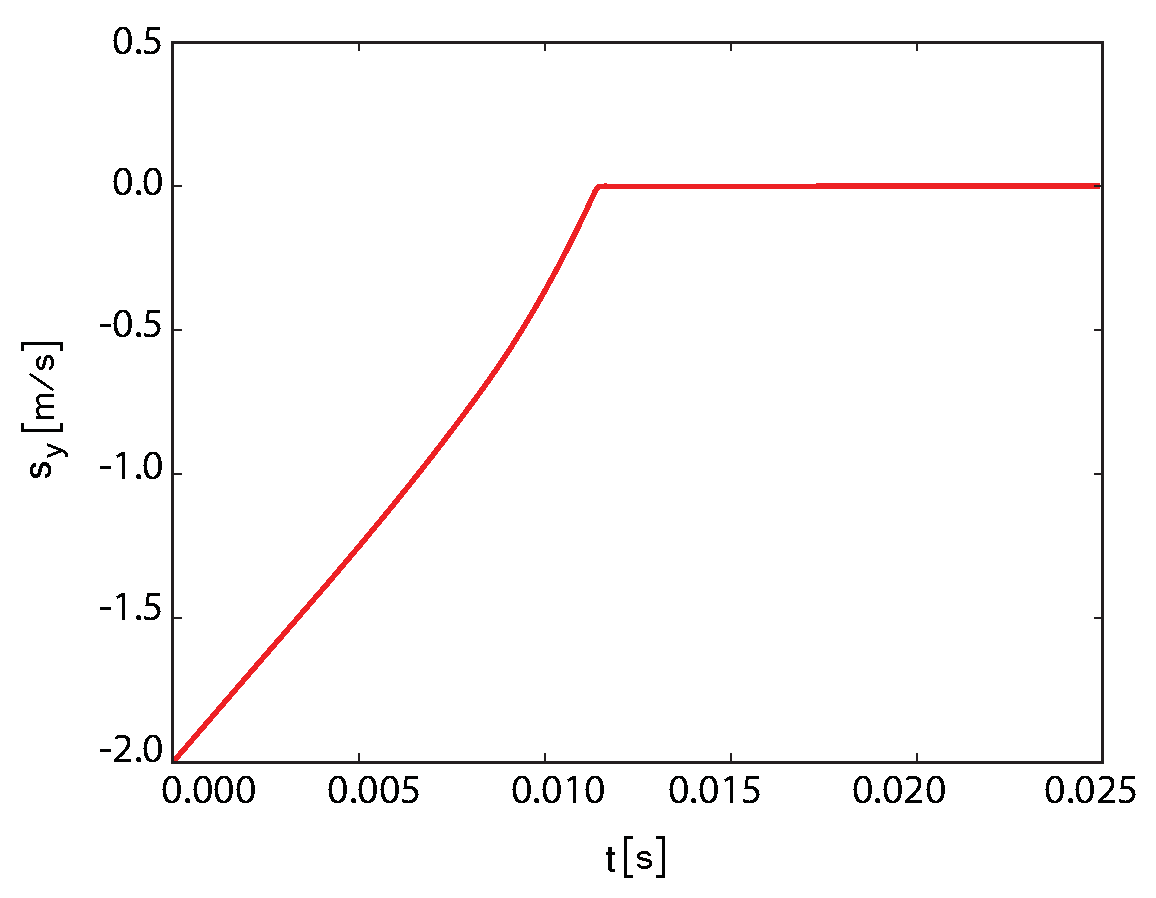
\includegraphics[scale=0.31]{../figures/sy2.pdf}  
	\caption{Variável $s_y$}
	\label{fig:sy2}
\end{figure}
\end{multicols}

Para fins de comparação, realizamos a simulação anterior mudando a lei de controle para a tradicional lei de Controle por Torque Computado com amortecimento crítico \cite{Craig}:
\begin{equation}
\mup = \hat{\mh}(\mq,\dot{\mq}\ssh) + \hat{\mH}(\mq)( \ddot{\mq}\ssh_d + 2 \lambda \dot{\me} + \lambda^2 \me )
\end{equation}

Escolhendo $\lambda = 40.0$, obtemos os seguintes resultados:

\begin{multicols}{2}
\begin{figure}[H]
	\centering
	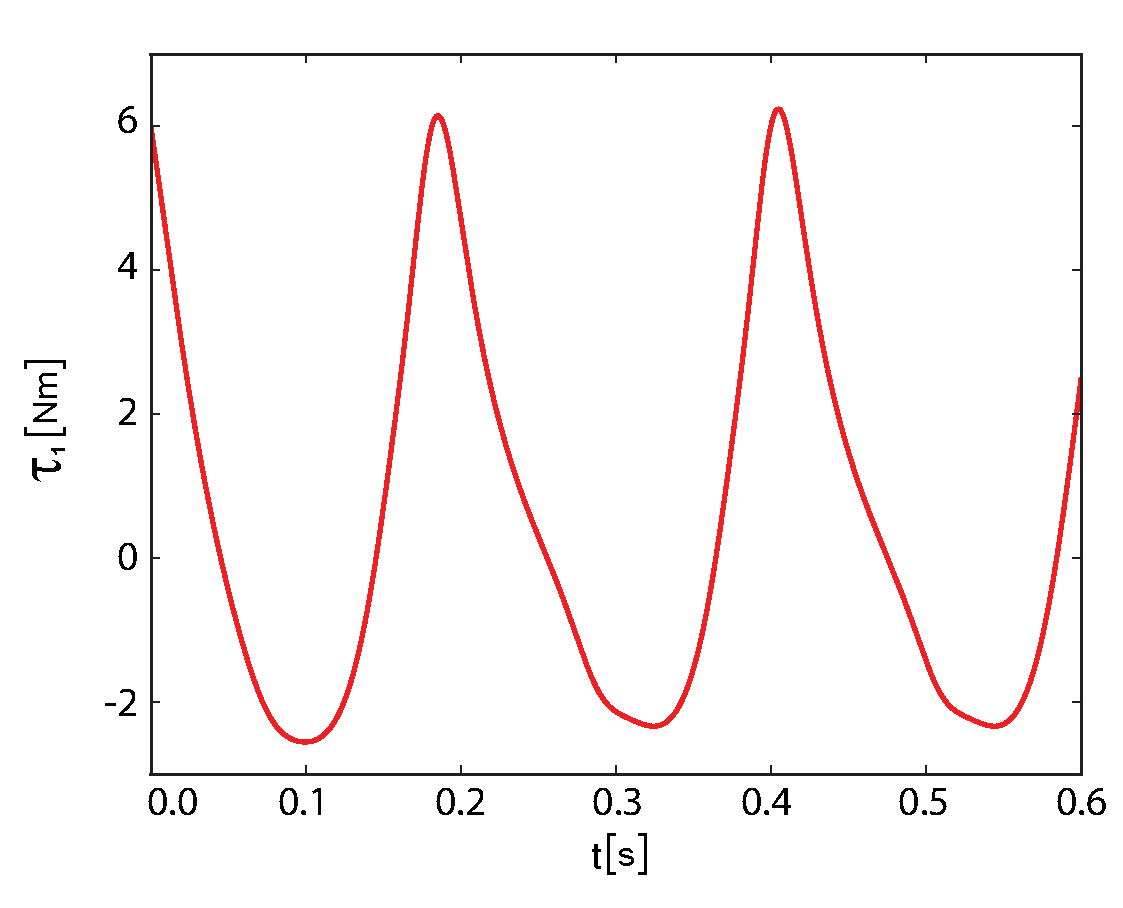
\includegraphics[scale=0.31]{../figures/Torque13.pdf}  
	\caption{Torque aplicado pelo atuador 1}
	\label{fig:Torque13}
\end{figure}

\begin{figure}[H]
	\centering
	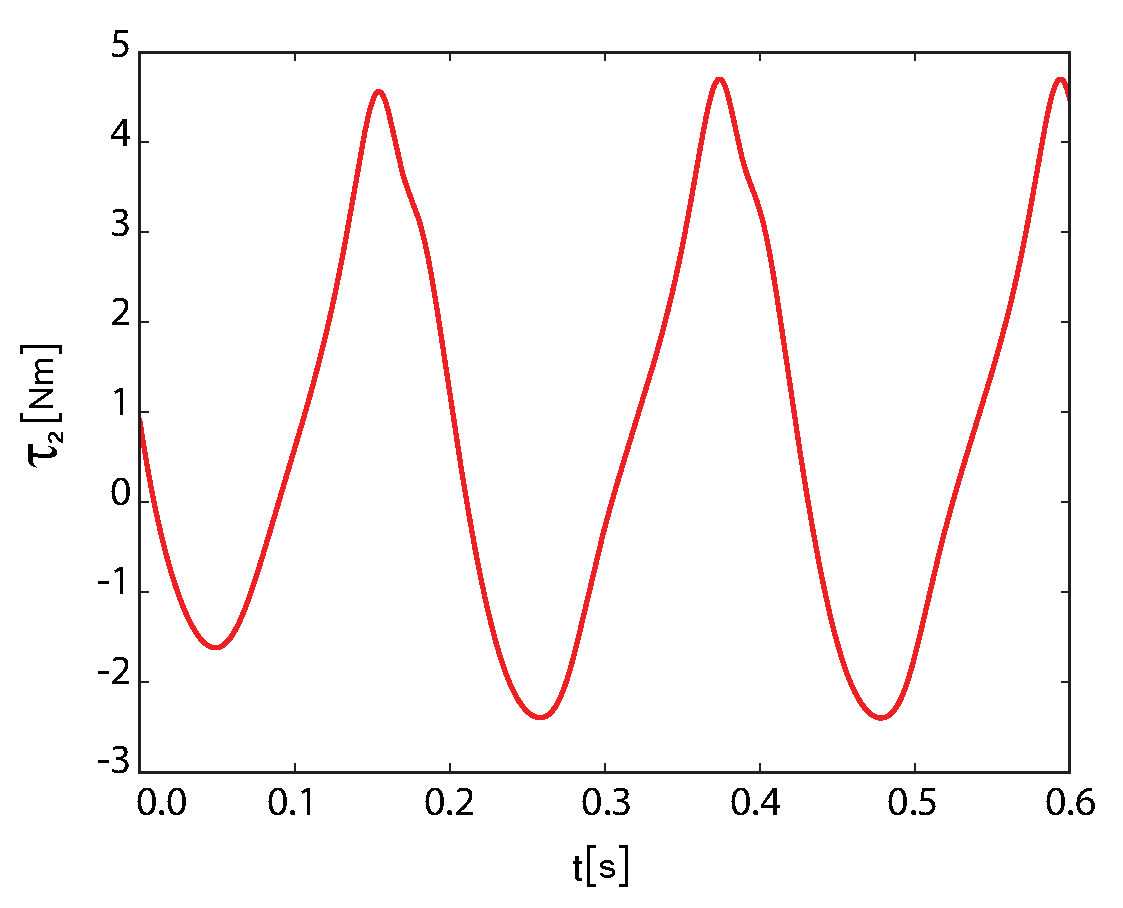
\includegraphics[scale=0.31]{../figures/Torque23.pdf}  
	\caption{Torque aplicado pelo atuador 2}
	\label{fig:Torque23}
\end{figure}
\end{multicols}
\begin{multicols}{2}
\begin{figure}[H]
	\centering
	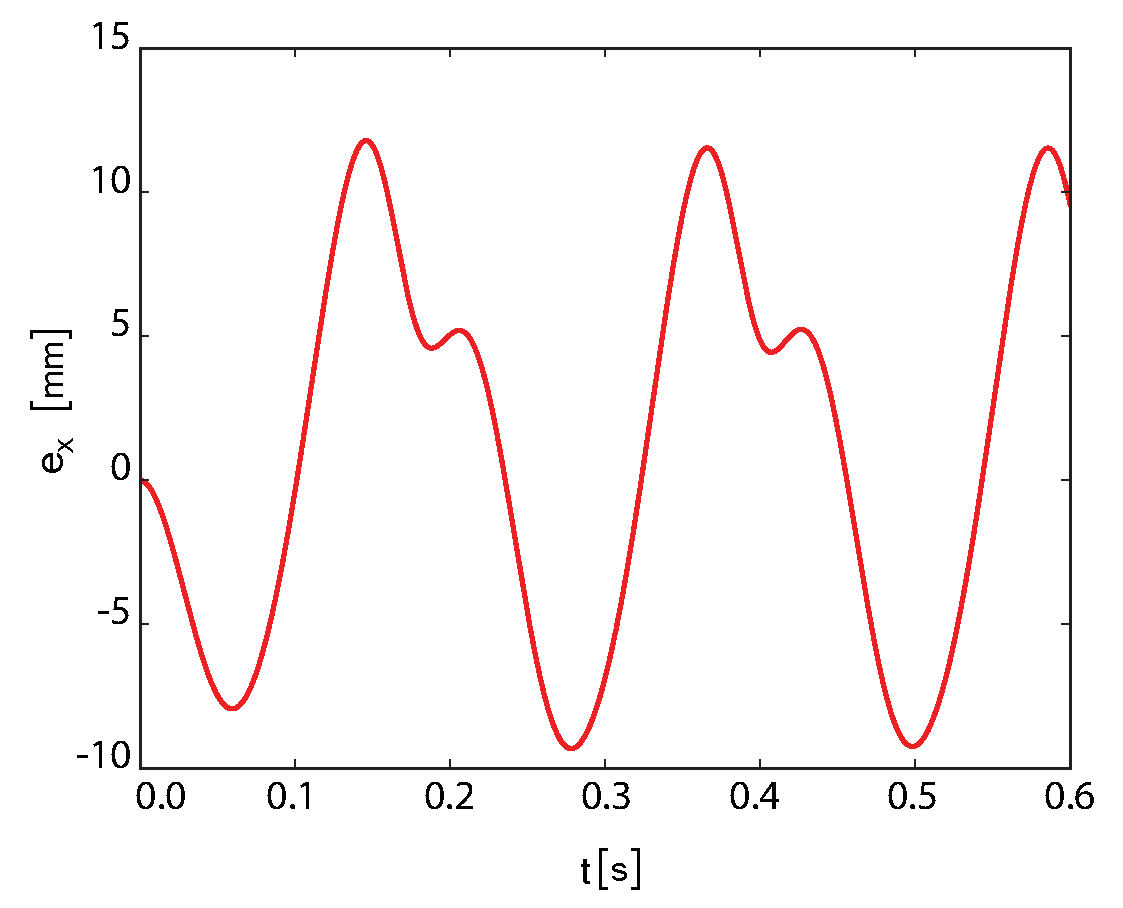
\includegraphics[scale=0.31]{../figures/ex3.pdf}  
	\caption{Erro de na coordenada $x$}
	\label{fig:ex3}
\end{figure}

\begin{figure}[H]
	\centering
	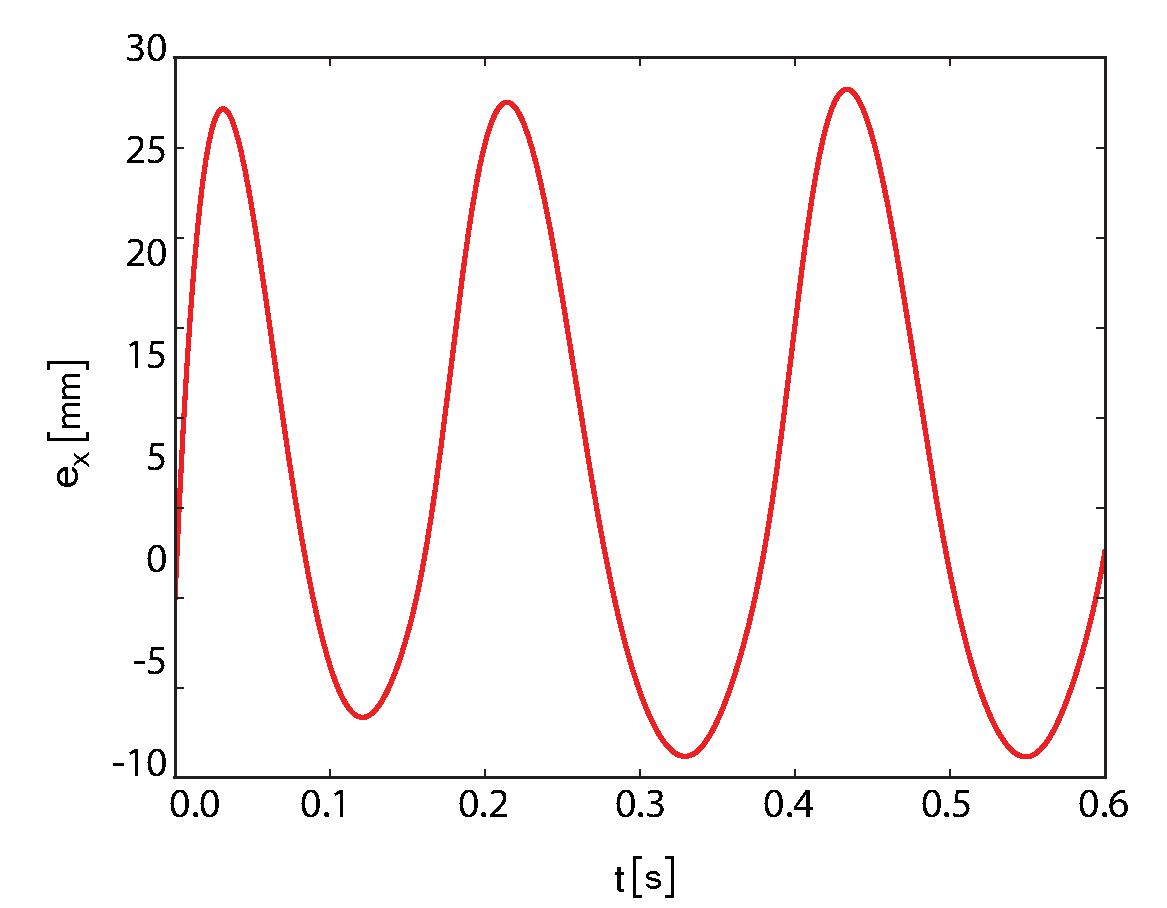
\includegraphics[scale=0.31]{../figures/ey3.pdf}  
	\caption{Erro de na coordenada $y$}
	\label{fig:ey3}
\end{figure}
\end{multicols}

Repare que a lei de Controle por Torque Computado não consegue seguir a trajetória de forma satisfatória, mantendo um erro em regime permanente oscilatório com pico $12 mm$ na coordenada $x$ e $27 mm$ na coordenada $y$.

\section{Ensaios Experimentais}

Nesta sessão, será descrita a bancada experimental e serão apresentados e discutidos os resultados experimentais do controle do mecanismo 5R utilizando 8 diferentes estratégias de controle

\subsection{Bancada experimental}

A bancada é constituída de:

\begin{itemize}
\item 2 motores DC modelo PM70 da AMETEK com as seguintes características:
\begin{itemize}
\item Corrente nominal de $13A$ 
\item Torque nominal de $0,5Nm$
\item Potência útil de $200W$
\item Tensão de alimentação de $24V$
\item Rotação nominal de $3600 rpm$
\item Peso de $1.80 kgf$ 
\end{itemize}
\item  2 enconders incrementais do modelo E40S com as seguintes características:
\begin{itemize}
\item Resolução de $5000 pulsos/volta$.
\item Tensão de alimentação de $12V$ a $24V$
\item 3 canais de saída A, B e Z
\end{itemize}
\item 1 driver modelo Pololu Dual VNH5019 Motor Driver Shield com as seguintes características.
\begin{itemize}
\item Tensões de operação: $5,5V$ a $24V$
\item Corrente de saída: até $12A$ contínuos (30A de pico)
\item Dois canais de saída para motor
\item Entrada de tensão do sistema pode ser tanto $5V$ quanto $3.3V$
\item Frequência de operação do PWM de até $20kHz$
\end{itemize}
\item 1 Microprocessador responsável pela execução das malhas de controle. O modelo utilizado foi o \textit{Raspberry Pi 2 Model B} com as seguintes características:
\begin{itemize}
\item Processador: quadcore ARMv7
\item 1GB RAM
\item alimentação de $5V$, $2A$
\end{itemize}
\end{itemize}

A arquitetura do sistema pode ser vista na figura \ref{arquitSistema}.

\begin{figure}[H]
    \centering
    \includegraphics[width=0.7\textwidth]{imagens/arqSist.png}
    \caption{Arquitetura do sistema}
    \label{arquitSistema}
\end{figure}

\subsection{Sistema de controle}

O sistema de controle é constituído de: 
\begin{itemize}
\item 2 derivadores para a obtencão da velocidade e aceleração dos motores
\item Cálculo da corrente que passa pelos motores
\item Malhas de controles, sendo uma linear (controle de corrente) e uma não linear 
\end{itemize} 

Pelo enconder obtemos a posição dos motores, com os derivadores obtemos a velocidade e a acelaração. Esses três sinais juntos com suas respectivas referências são utilizadas na malha de controle não linear. A velocidade, junto com a tensão que é enviada ao motor são utilizadas para calcular a corrente que passa no motor. Com o erro entre o valor calculado e a corrente de referência, o controlador calcula e envia a tensão ao motor. A arquitetura pode ser visualizada na figura \ref{arquitControle}.


\begin{figure}[H]
    \centering
    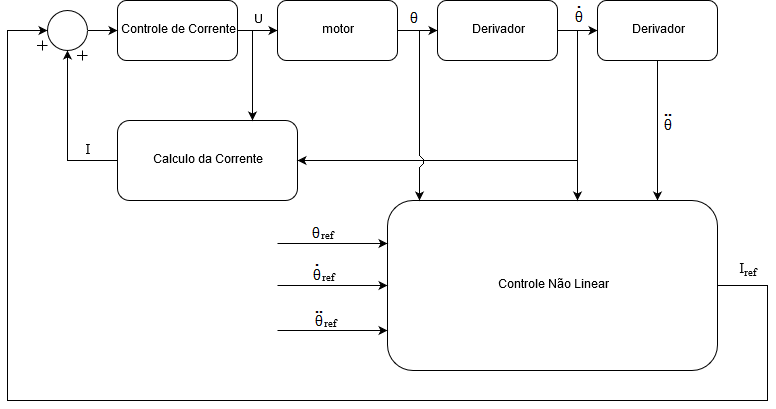
\includegraphics[width=0.8\textwidth]{imagens/ArqControle.png}
    \caption{Arquitetura de controle}
    \label{arquitControle}
\end{figure}

\subsection{Derivador}
\label{derivador}

A partir da posição angular obtida através da leitura do encoder, é possível determinar a velocidade usando um derivador numérico. Uma das formas de se obter o derivador é pelo método das diferenças finitas:

\begin{equation}
\dot{x}_k = \frac{x_k - x_{k-1}}{T}
\end{equation}

No entanto, como há ruídos nos sinais obtidos, a utilização  do método das diferenças finitas amplifica os ruídos de alta frequência. Diante disso, optamos por utilizar os derivadores em série com filtros passa-baixa tipo Bessel de segunda ordem (para o cálculo da velocidade a partir da posição) e oitava ordem (para o cálculo da aceleração a partir da velocidade).

\subsection{Cálculo da corrente}

Para o cálculo da corrente foi considerada a equacação da dinâmica elétrica do motor \eqref{eq:DinEletrica_rot}:

\begin{equation}
\tag{\ref{eq:DinEletrica_rot}}
	   u = L \frac{di}{dt} + R i + k_{e} \omega
\end{equation}

A dinâmica elétrica é muito mais rápida que a mecânica, portanto ela será desprezada ($\frac{di}{dt} = 0$). Com isso, obtemos a seguinte equação para o cálculo da corrente:

\begin{equation}
\label{corrente}
I = \frac{u - k_e \omega}{R}
\end{equation}

\subsection{Parâmetros do sistema}

\begin{table}[H] 
\centering
\caption{Parâmetros da cadeia 1}
\label{parametrosCadeia1}
\begin{tabular}{l|l|l}
Parâmetros   & Valores                  & Unidades      \\ \hline
$l_0$        & $0.050$                     & $m$        \\
$l_1$        & $0.120$                     & $m$        \\
$l_2$        & $0.160$                     & $m$        \\
$l_{g1}$     & $0.060$                     & $m$        \\
$l_{g2}$     & $0.078$                    & $m$        \\
$m_1$        & $0.062$                    & $kg$       \\
$m_2$        & $0.124$                    & $kg$       \\
$J_{z1}$     & $1.073 \cdot 10^{-4}$    & $kg.m^{2}$ \\
$J_{z2}$     & $4.380 \cdot 10^{-4}$    & $kg.m^{2}$ \\
\end{tabular}
\end{table} 

\begin{table}[H] 
\centering
\caption{Parâmetros da cadeia 2}
\label{parametrosCadeia2}
\begin{tabular}{l|l|l}
Parâmetros   & Valores                    & Unidades   \\ \hline
$l_0$        & $0.050$                    & $m$        \\
$l_1$        & $0.120$                    & $m$        \\
$l_2$        & $0.160$                    & $m$        \\
$l_{g1}$     & $0.060$                    & $m$        \\
$l_{g2}$     & $0.058$                    & $m$        \\
$m_1$        & $0.062$                    & $kg$       \\
$m_2$        & $0.097$                    & $kg$       \\
$J_{z1}$     & $2.960   \cdot 10^{-4}$    & $kg.m^{2}$ \\
$J_{z2}$     & $9.800   \cdot 10^{-4}$    & $kg.m^{2}$ \\
\end{tabular}
\end{table}

\begin{table}[H] 
\centering
\caption{Parâmetros do Motor 1}
\label{parametrosMotor}
\begin{tabular}{l|l|l}
Parâmetros  & Valores               & Unidades   \\ \hline
$R$         & $1.101$               & $\Omega$   \\
$L$         & $0.667$               & $mH$       \\
$b$         & $1.226 \cdot 10^{-4}$ & $N s$      \\
$k_{t}$     & $5.598 \cdot 10^{-2}$ & $Nm/A$     \\
$\gmu$      & $4.357 \cdot 10^{-2}$ & $Nm$       \\
$k_{e}$     & $5.138 \cdot 10^{-2}$ & $V s/rad$  \\
$J$         & $1.469 \cdot 10^{-4}$ & $kg.m^{2}$
\end{tabular}
\end{table} 

\begin{table}[H] 
\centering
\caption{Parâmetros do Motor 2}
\label{parametrosMotor2}
\begin{tabular}{l|l|l}
Parâmetros & Valores               & Unidades   \\ \hline
$R$        & $0.829$               & $\Omega$   \\
$L$        & $0.667$               & $mH$       \\
$b$        & $2.039 \cdot 10^{-4}$ & $N s$      \\
$k_{t}$    & $5.666 \cdot 10^{-2}$ & $Nm/A$     \\
$\gmu$     & $4.992 \cdot 10^{-2}$ & $Nm$        \\
$k_{e}$    & $5.200 \cdot 10^{-2}$ & $V s/rad$  \\
$J$        & $1.887 \cdot10^{-4}$  & $kg.m^{2}$
\end{tabular}
\end{table}

\subsection{Trajetórias de referência}

A primeira trajetória a ser realizada é uma trajetória circular com período de 1 segundo. Serão realizados 8 ciclos seguidos de uma parada repentina. Sua expressão é dada por:

\begin{equation}
\begin{cases}
x_d(t) = -0.05 \cos(6.28 t) \\
y_d(t) = 0.158 - 0.05 \sin(6.28 t) \\
\end{cases}
\end{equation}

A segunda trajetória a ser realizada é uma trajetória triangular cujas coordenadas dos vértices (em metros) são:

\begin{equation} \label{eq:zeroMaquina}
\mx_1 = \begin{bmatrix}
-0.002 & 0.108 
\end{bmatrix}^\msT
\end{equation}
\begin{equation}
\mx_2 = \begin{bmatrix}
0.050 & 0.258 
\end{bmatrix}^\msT
\end{equation}
\begin{equation}
\mx_3 = \begin{bmatrix}
-0.050 & 0.258 
\end{bmatrix}^\msT
\end{equation}

Serão realizados 2 ciclos, sendo que cada lado do triângulo é percorrido em $0.75s$, e sendo o trecho I de $\mx_1$ a $\mx_2$, o trecho II de $\mx_2$ a $\mx_3$, e o trecho III de $\mx_3$ a $\mx_1$. Depois de completar os 2 ciclos, será feita uma parada suave. Em cada lado do triângulo, é parametrizada uma trajetória polinomial de sétima ordem, na qual é imposta a posição inicial e final, velocidade nula, aceleração nula e tranco nulo no início e no final da trajetória. A expressão do polinômio é dada por:

\begin{equation}
\mx(\mathfrak{t}) = \mx_0 + (\mx_f - \mx_0) (35 \mathfrak{t}^4 - 84 \mathfrak{t}^5 + 70 \mathfrak{t}^6 - 20 \mathfrak{t}^7)
\end{equation}

Sendo $\mx$ a posição atual, $\mx_0$ a posição inicial, $\mx_f$ a posição final, e $\mathfrak{t}$ a fração do tempo decorrido em relação ao tempo total da trajetória (repare que $\mx(1) = \mx_f$).

\subsection{Condições iniciais}

O mecanismo sempre parte do repouso na posição $\mx_1$, dada pela equação \eqref{eq:zeroMaquina}

\subsection{Parâmetros dos controladors}

\begin{table}[H] 
\centering
\caption{Parâmetros dos controladores: espaço das juntas - trajetória circular}
\label{tab:parametrosControleAtuadoresCirculo}
\begin{tabular}{l|l|l|l|l|l}
Estratégia & $\lambda [rad/s]$  & $m^*[kg.m^2]$ & $\phi[rad/s^2]$   & $k_1[rad/s^2]$ & $k_2[rad/s^2]$ \\ \hline
PDq        & $35$               & $3.58 \cdot 10^{-3}$  & -         & -              & -              \\
PDMDq      & $35$               & $3.58 \cdot 10^{-3}$  & $20$      & $200$          & $200$          \\
TCq        & $60$               & -                     & -         & -              & -              \\
TCMDq      & $60$               & -                     & $20$      & $363$          & $363$          \\
\end{tabular}
\end{table}

\begin{table}[H] 
\centering
\caption{Parâmetros dos controladores: espaço das juntas - trajetória triangular}
\label{tab:parametrosControleAtuadoresTriangulo}
\begin{tabular}{l|l|l|l|l|l}
Estratégia & $\lambda [rad/s]$  & $m^*[kg.m^2]$         & $\phi[rad/s^2]$   & $k_1[rad/s^2]$ & $k_2[rad/s^2]$ \\ \hline
PDq        & $25$               & $3.58 \cdot 10^{-3}$  & -         & -              & -              \\
PDMDq      & $25$               & $3.58 \cdot 10^{-3}$  & $90$      & $200$          & $200$          \\
TCq        & $60$               & -                     & -         & -              & -              \\
TCMDq      & $60$               & -                     & $20$      & $363$          & $363$          \\
\end{tabular}
\end{table}

\begin{table}[H] 
\centering
\caption{Parâmetros dos controladores: espaço da tarefa}
\label{tab:parametrosControleEfetuador}
\begin{tabular}{l|l|l|l|l|l}
Estratégia & $\lambda [rad/s]$  & $m^*[kg]$ & $\phi[m/s^2]$ & $k_1[m/s^2]$ & $k_2[m/s^2]$ \\ \hline
PDx        & $70$               & $0.207$   & -             & -            & -            \\
PDMDx      & $70$               & $0.207$   & $6$           & $70$         & $0$          \\
TCx        & $60$               & -         & -             & -            & -            \\
TCMDx      & $60$               & -         & $6$           & $103$        & $0$          \\
\end{tabular}
\end{table}

\newpage

\subsection{Resultados experimentais}

\subsubsection{PDq - Trajetória circular}

\begin{figure}[H]
	\centering
	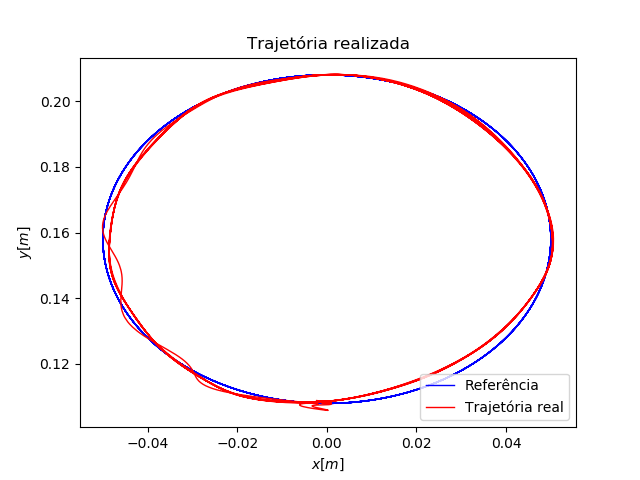
\includegraphics[scale=0.39]{../../../Experimental/Aquisicoes/PIDt_circulo/xy.png}  
	\caption{Trajetória realizada}
	\label{fig:PIDq_circulo_xy}
\end{figure}
\begin{multicols}{2}
\begin{figure}[H]
	\centering
	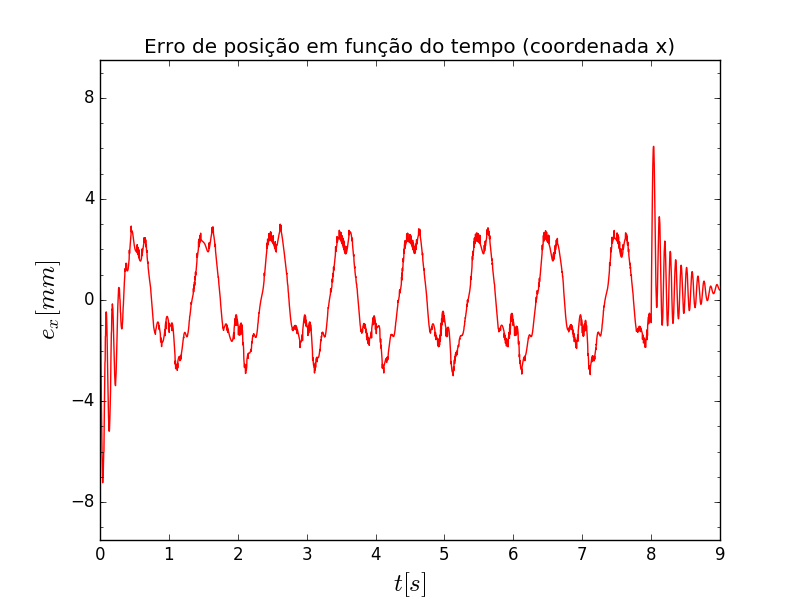
\includegraphics[scale=0.39]{../../../Experimental/Aquisicoes/PIDt_circulo/ex.png}  
	\caption{Erro de controle $e_x$}
	\label{fig:PIDq_circulo_ex}
\end{figure}
\begin{figure}[H]
	\centering
	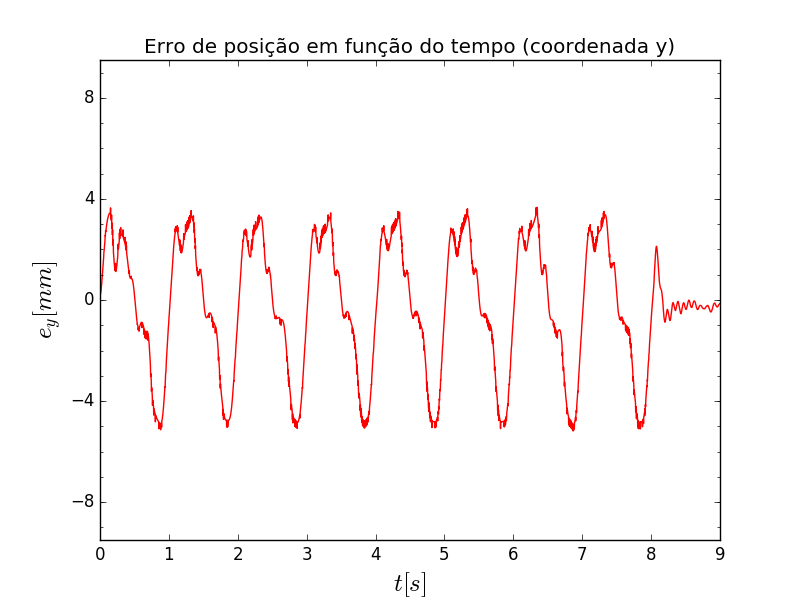
\includegraphics[scale=0.39]{../../../Experimental/Aquisicoes/PIDt_circulo/ey.png}  
	\caption{Erro de controle $e_y$}
	\label{fig:PIDq_circulo_ey}
\end{figure}
\end{multicols}
\begin{multicols}{2}
\begin{figure}[H]
	\centering
	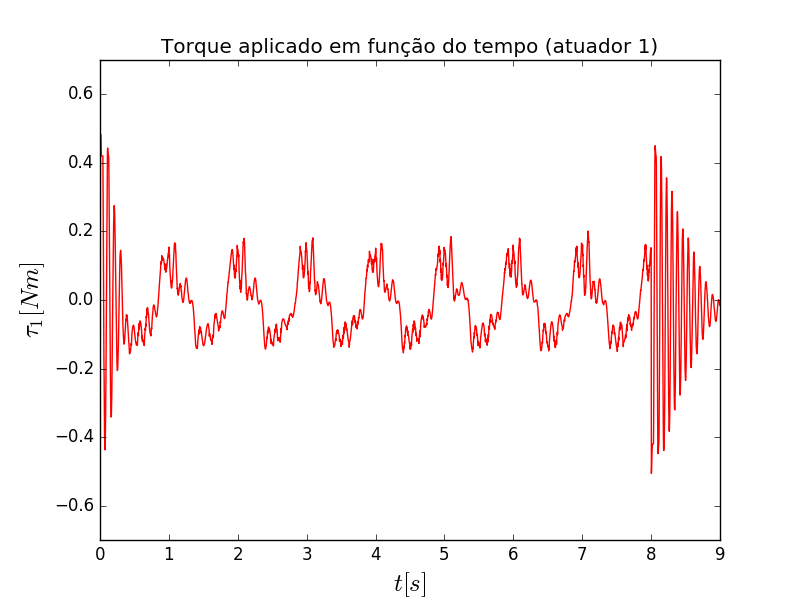
\includegraphics[scale=0.39]{../../../Experimental/Aquisicoes/PIDt_circulo/tau1.png}  
	\caption{Esforço de controle $\tau_1$}
	\label{fig:PIDq_circulo_tau1}
\end{figure}
\begin{figure}[H]
	\centering
	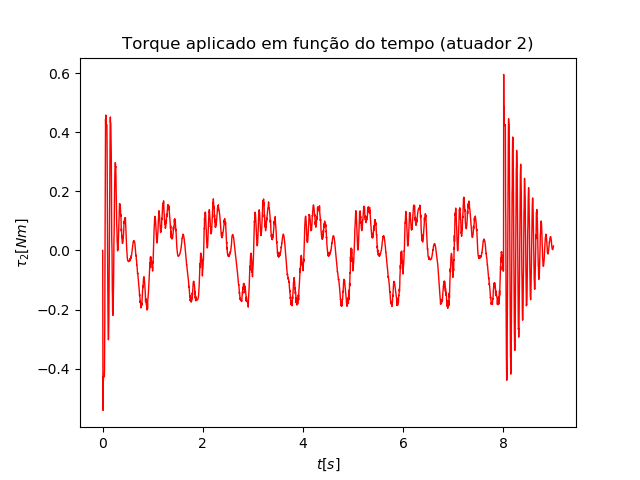
\includegraphics[scale=0.39]{../../../Experimental/Aquisicoes/PIDt_circulo/tau2.png}  
	\caption{Esforço de controle $\tau_2$}
	\label{fig:PIDq_circulo_tau2}
\end{figure}
\end{multicols}

\subsubsection{PDMDq - Trajetória circular}

\begin{figure}[H]
	\centering
	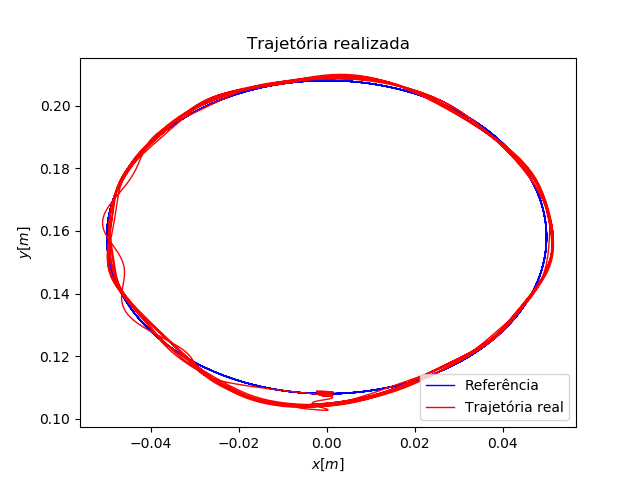
\includegraphics[scale=0.39]{../../../Experimental/Aquisicoes/PIDSMCt_circulo/xy.png}  
	\caption{Trajetória realizada}
	\label{fig:PIDSMCq_circulo_xy}
\end{figure}
\begin{multicols}{2}
\begin{figure}[H]
	\centering
	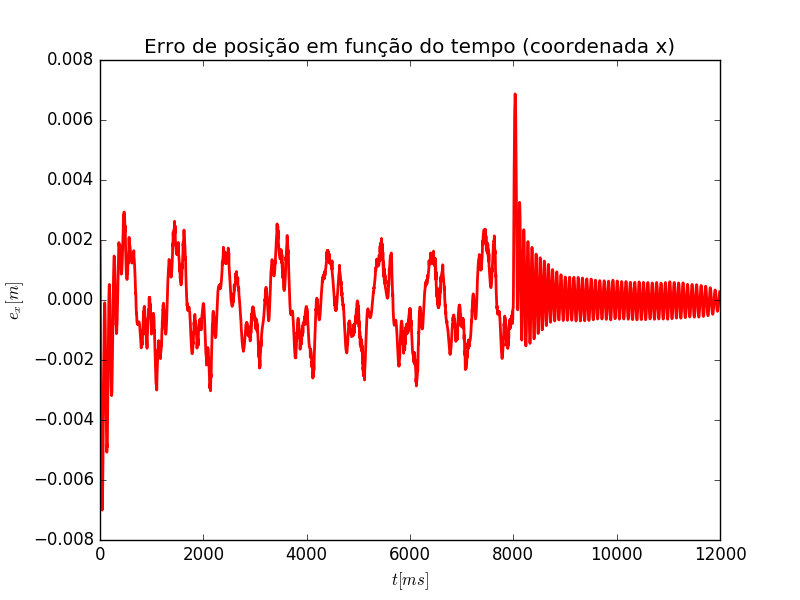
\includegraphics[scale=0.39]{../../../Experimental/Aquisicoes/PIDSMCt_circulo/ex.png}  
	\caption{Erro de controle $e_x$}
	\label{fig:PIDSMCq_circulo_ex}
\end{figure}
\begin{figure}[H]
	\centering
	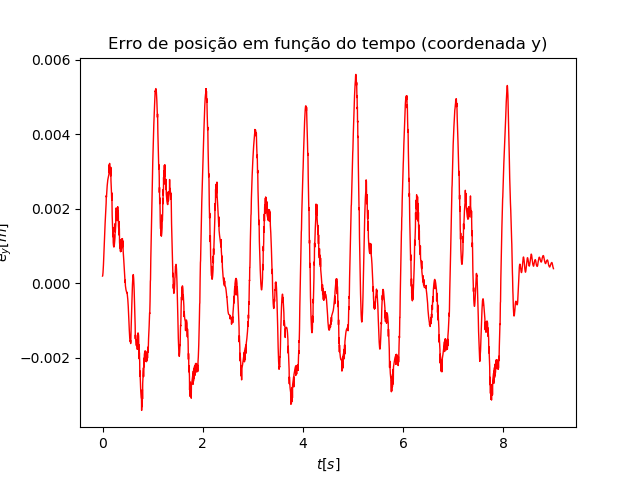
\includegraphics[scale=0.39]{../../../Experimental/Aquisicoes/PIDSMCt_circulo/ey.png}  
	\caption{Erro de controle $e_y$}
	\label{fig:PIDSMCq_circulo_ey}
\end{figure}
\end{multicols}
\begin{multicols}{2}
\begin{figure}[H]
	\centering
	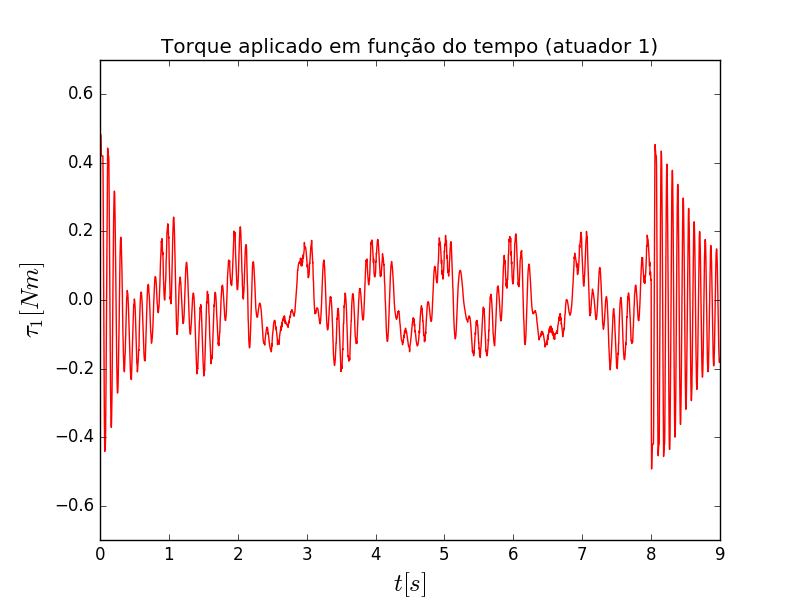
\includegraphics[scale=0.39]{../../../Experimental/Aquisicoes/PIDSMCt_circulo/tau1.png}  
	\caption{Esforço de controle $\tau_1$}
	\label{fig:PIDSMCq_circulo_tau1}
\end{figure}
\begin{figure}[H]
	\centering
	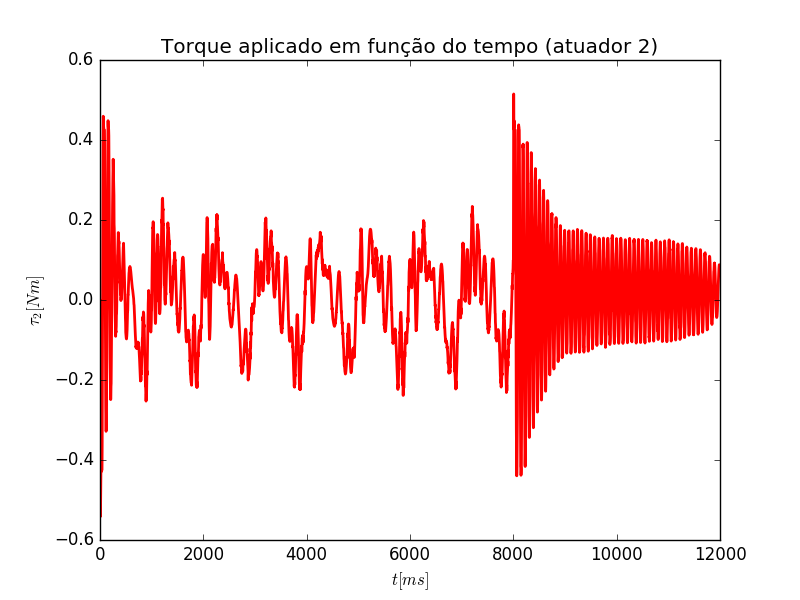
\includegraphics[scale=0.39]{../../../Experimental/Aquisicoes/PIDSMCt_circulo/tau2.png}  
	\caption{Esforço de controle $\tau_2$}
	\label{fig:PIDSMCq_circulo_tau2}
\end{figure}
\end{multicols}

\subsubsection{TCq - Trajetória circular}

\begin{figure}[H]
	\centering
	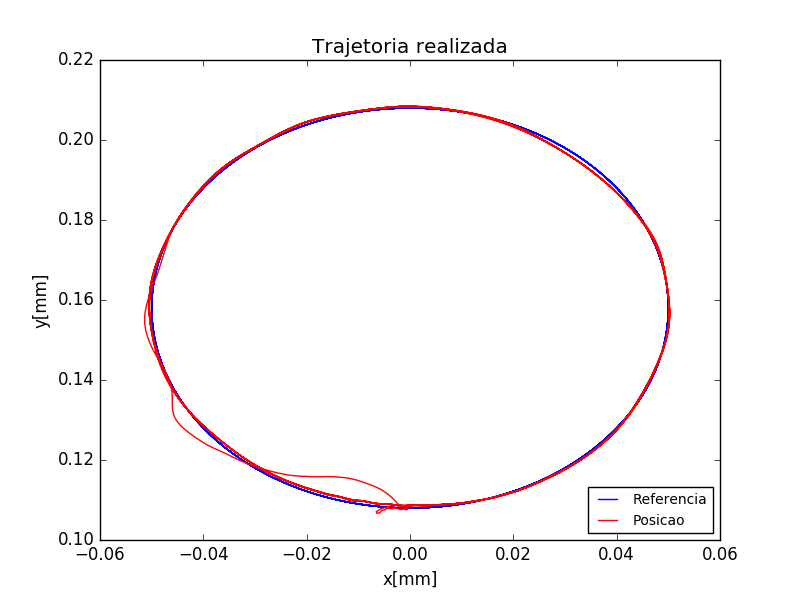
\includegraphics[scale=0.39]{../../../Experimental/Aquisicoes/CTCt_circulo/xy.png}  
	\caption{Trajetória realizada}
	\label{fig:CTCq_circulo_xy}
\end{figure}
\begin{multicols}{2}
\begin{figure}[H]
	\centering
	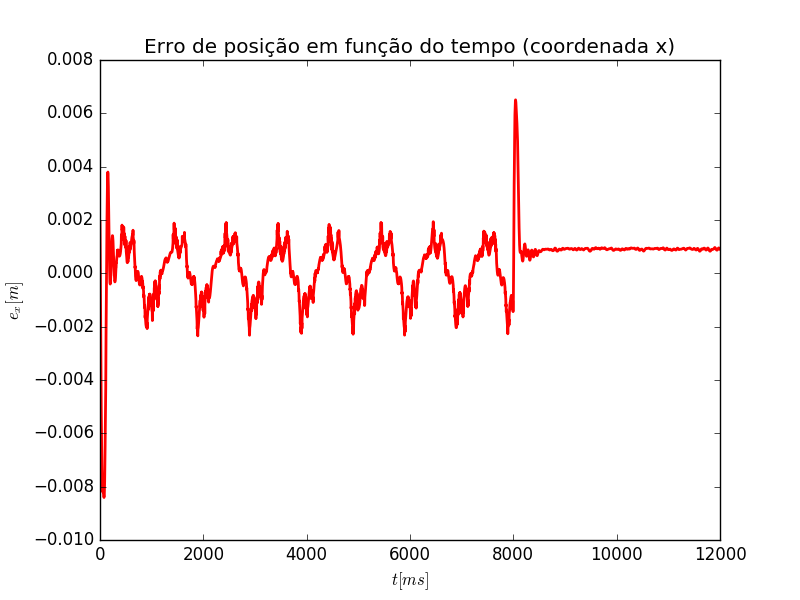
\includegraphics[scale=0.39]{../../../Experimental/Aquisicoes/CTCt_circulo/ex.png}  
	\caption{Erro de controle $e_x$}
	\label{fig:CTCq_circulo_ex}
\end{figure}
\begin{figure}[H]
	\centering
	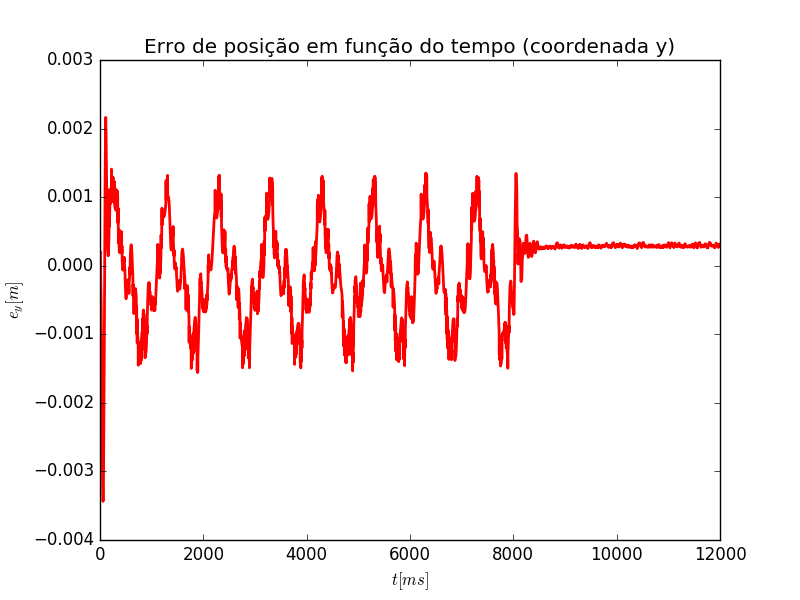
\includegraphics[scale=0.39]{../../../Experimental/Aquisicoes/CTCt_circulo/ey.png}  
	\caption{Erro de controle $e_y$}
	\label{fig:CTCq_circulo_ey}
\end{figure}
\end{multicols}
\begin{multicols}{2}
\begin{figure}[H]
	\centering
	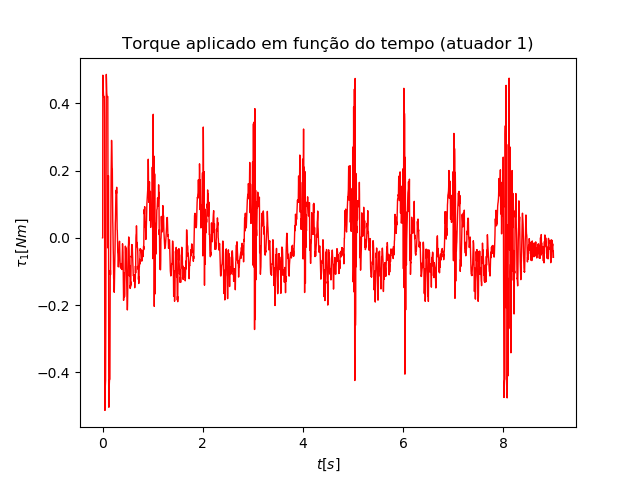
\includegraphics[scale=0.39]{../../../Experimental/Aquisicoes/CTCt_circulo/tau1.png}  
	\caption{Esforço de controle $\tau_1$}
	\label{fig:CTCq_circulo_tau1}
\end{figure}
\begin{figure}[H]
	\centering
	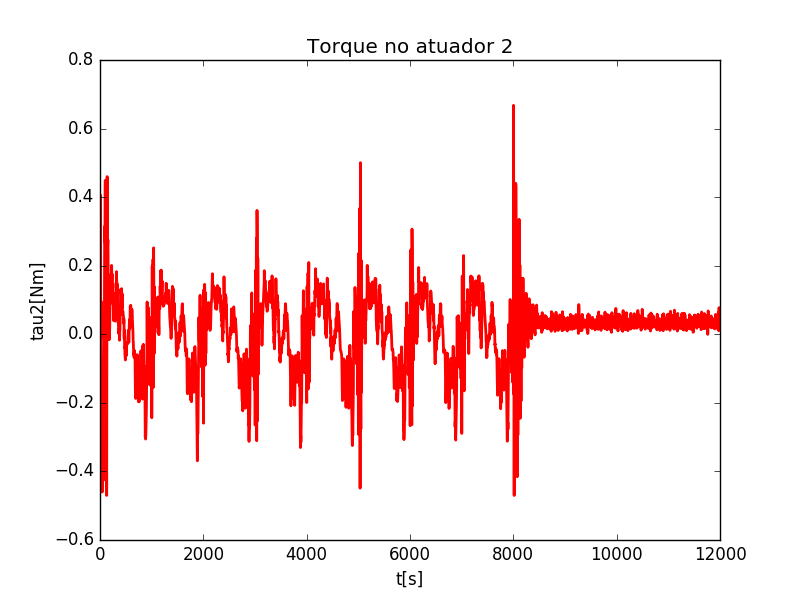
\includegraphics[scale=0.39]{../../../Experimental/Aquisicoes/CTCt_circulo/tau2.png}  
	\caption{Esforço de controle $\tau_2$}
	\label{fig:CTCq_circulo_tau2}
\end{figure}
\end{multicols}

\subsubsection{TCMDq - Trajetória circular}

\begin{figure}[H]
	\centering
	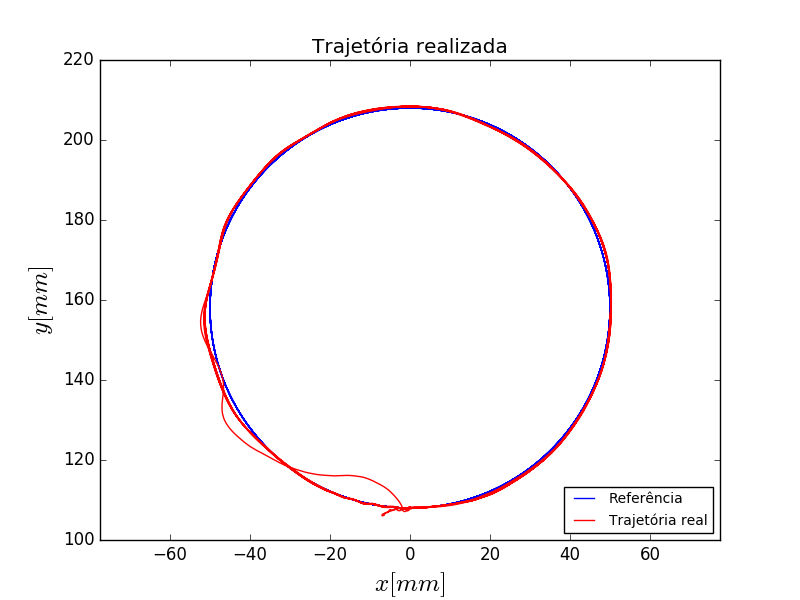
\includegraphics[scale=0.39]{../../../Experimental/Aquisicoes/SMCt_circulo/xy.png}  
	\caption{Trajetória realizada}
	\label{fig:SMCq_circulo_xy}
\end{figure}
\begin{multicols}{2}
\begin{figure}[H]
	\centering
	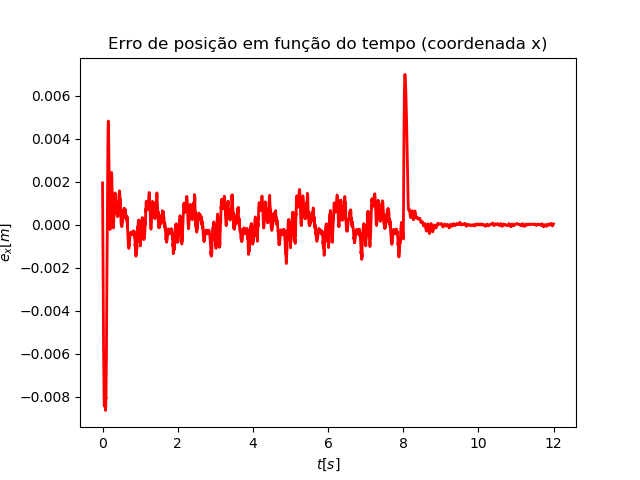
\includegraphics[scale=0.39]{../../../Experimental/Aquisicoes/SMCt_circulo/ex.png}  
	\caption{Erro de controle $e_x$}
	\label{fig:SMCq_circulo_ex}
\end{figure}
\begin{figure}[H]
	\centering
	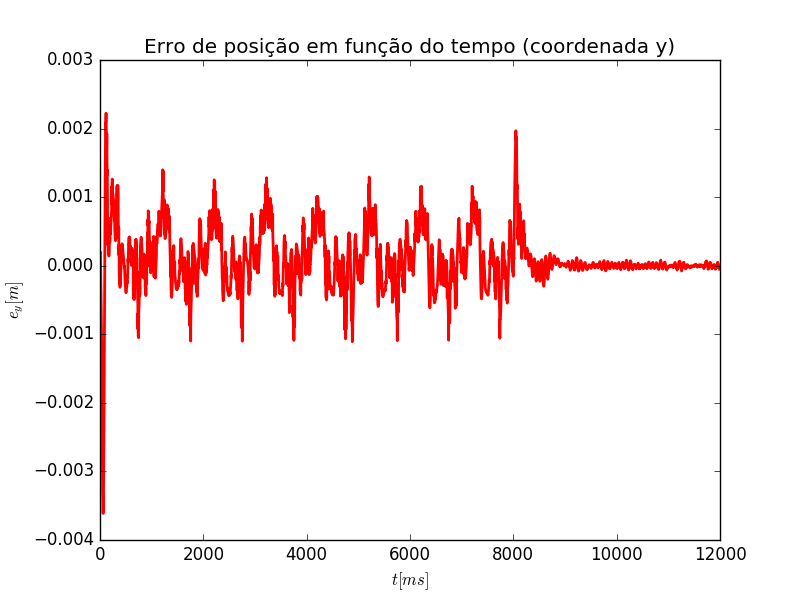
\includegraphics[scale=0.39]{../../../Experimental/Aquisicoes/SMCt_circulo/ey.png}  
	\caption{Erro de controle $e_y$}
	\label{fig:SMCq_circulo_ey}
\end{figure}
\end{multicols}
\begin{multicols}{2}
\begin{figure}[H]
	\centering
	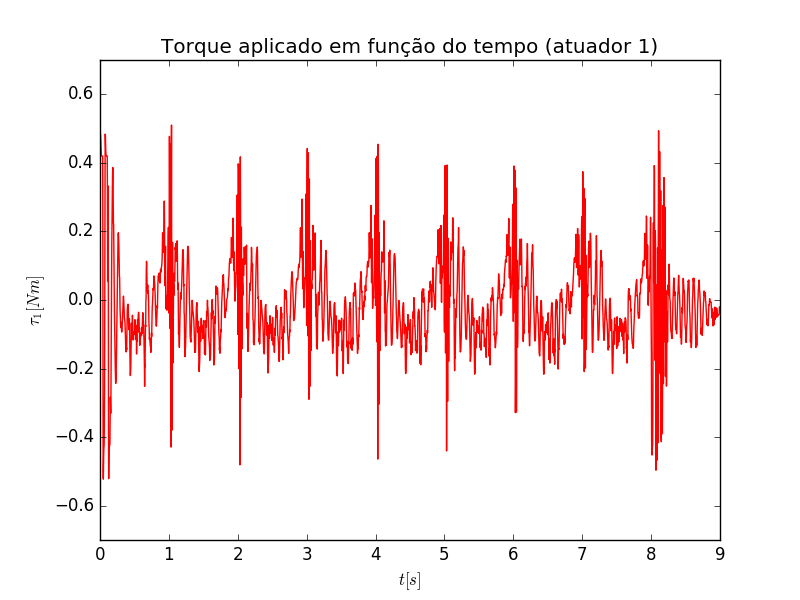
\includegraphics[scale=0.39]{../../../Experimental/Aquisicoes/SMCt_circulo/tau1.png}  
	\caption{Esforço de controle $\tau_1$}
	\label{fig:SMCq_circulo_tau1}
\end{figure}
\begin{figure}[H]
	\centering
	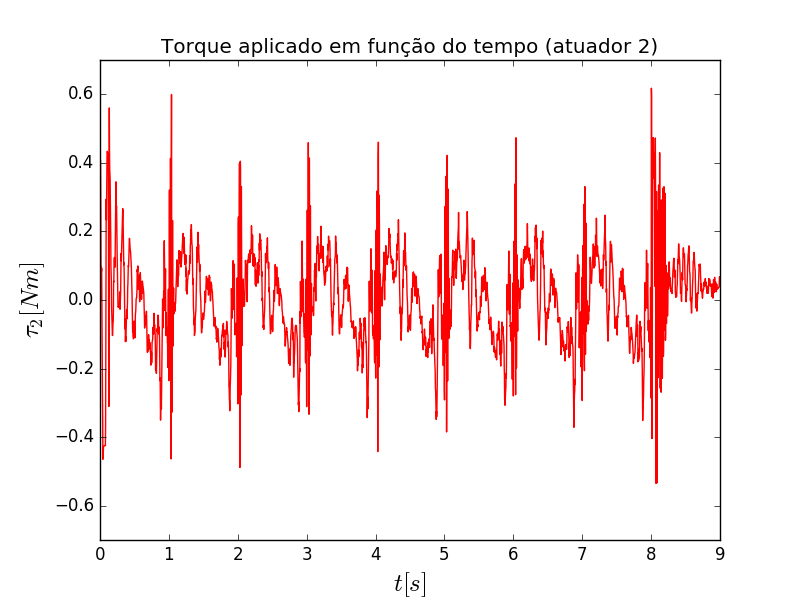
\includegraphics[scale=0.39]{../../../Experimental/Aquisicoes/SMCt_circulo/tau2.png}  
	\caption{Esforço de controle $\tau_2$}
	\label{fig:SMCq_circulo_tau2}
\end{figure}
\end{multicols}


\subsubsection{PDx - Trajetória circular}

\begin{figure}[H]
	\centering
	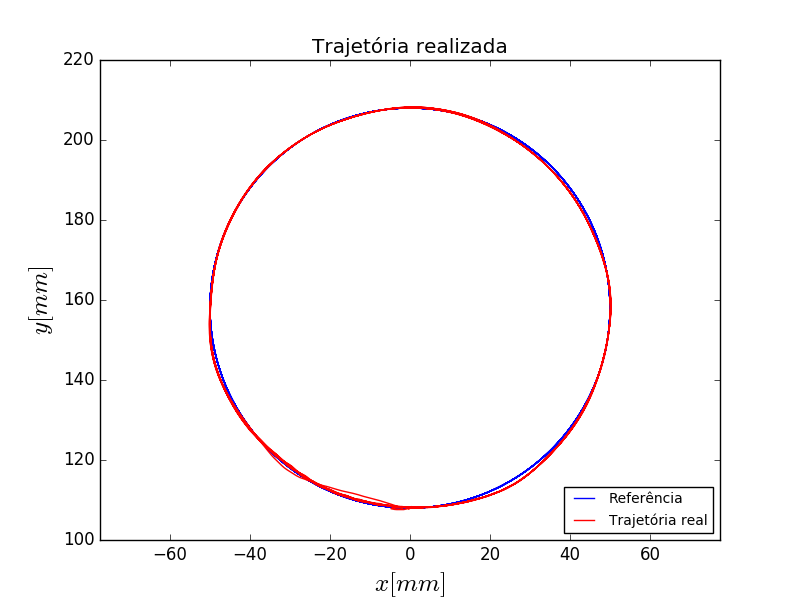
\includegraphics[scale=0.39]{../../../Experimental/Aquisicoes/PIDx_circulo/xy.png}  
	\caption{Trajetória realizada}
	\label{fig:PIDx_circulo_xy}
\end{figure}
\begin{multicols}{2}
\begin{figure}[H]
	\centering
	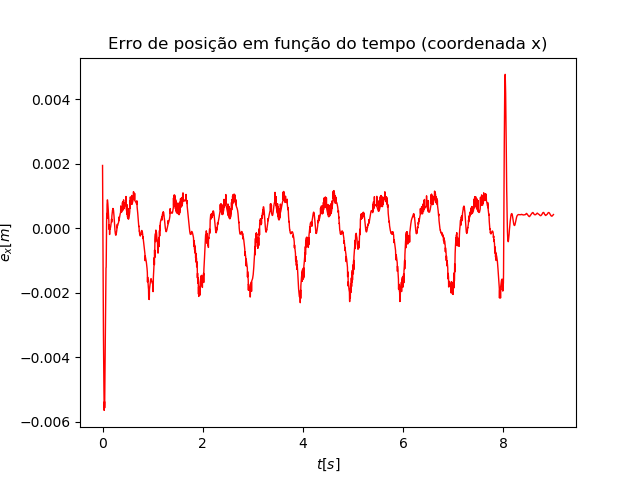
\includegraphics[scale=0.39]{../../../Experimental/Aquisicoes/PIDx_circulo/ex.png}  
	\caption{Erro de controle $e_x$}
	\label{fig:PIDx_circulo_ex}
\end{figure}
\begin{figure}[H]
	\centering
	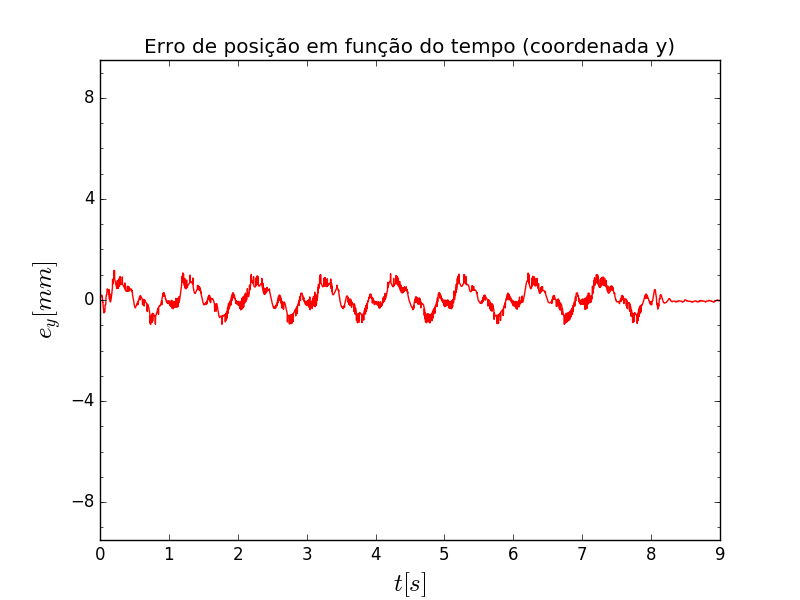
\includegraphics[scale=0.39]{../../../Experimental/Aquisicoes/PIDx_circulo/ey.png}  
	\caption{Erro de controle $e_y$}
	\label{fig:PIDx_circulo_ey}
\end{figure}
\end{multicols}
\begin{multicols}{2}
\begin{figure}[H]
	\centering
	\includegraphics[scale=0.39]{../../../Experimental/Aquisicoes/PIDx_circulo/tau1.png}  
	\caption{Esforço de controle $\tau_1$}
	\label{fig:PIDx_circulo_tau1}
\end{figure}
\begin{figure}[H]
	\centering
	\includegraphics[scale=0.39]{../../../Experimental/Aquisicoes/PIDx_circulo/tau2.png}  
	\caption{Esforço de controle $\tau_2$}
	\label{fig:PIDx_circulo_tau2}
\end{figure}
\end{multicols}

\subsubsection{PDMDx - Trajetória circular}

\begin{figure}[H]
	\centering
	\includegraphics[scale=0.39]{../../../Experimental/Aquisicoes/PIDSMCx_circulo/xy.png}  
	\caption{Trajetória realizada}
	\label{fig:PIDSMCx_circulo_xy}
\end{figure}
\begin{multicols}{2}
\begin{figure}[H]
	\centering
	\includegraphics[scale=0.39]{../../../Experimental/Aquisicoes/PIDSMCx_circulo/ex.png}  
	\caption{Erro de controle $e_x$}
	\label{fig:PIDSMCx_circulo_ex}
\end{figure}
\begin{figure}[H]
	\centering
	\includegraphics[scale=0.39]{../../../Experimental/Aquisicoes/PIDSMCx_circulo/ey.png}  
	\caption{Erro de controle $e_y$}
	\label{fig:PIDSMCx_circulo_ey}
\end{figure}
\end{multicols}
\begin{multicols}{2}
\begin{figure}[H]
	\centering
	\includegraphics[scale=0.39]{../../../Experimental/Aquisicoes/PIDSMCx_circulo/tau1.png}  
	\caption{Esforço de controle $\tau_1$}
	\label{fig:PIDSMCx_circulo_tau1}
\end{figure}
\begin{figure}[H]
	\centering
	\includegraphics[scale=0.39]{../../../Experimental/Aquisicoes/PIDSMCx_circulo/tau2.png}  
	\caption{Esforço de controle $\tau_2$}
	\label{fig:PIDSMCx_circulo_tau2}
\end{figure}
\end{multicols}

\subsubsection{TCx - Trajetória circular}

\begin{figure}[H]
	\centering
	\includegraphics[scale=0.39]{../../../Experimental/Aquisicoes/CTCx_circulo/xy.png}  
	\caption{Trajetória realizada}
	\label{fig:CTCx_circulo_xy}
\end{figure}
\begin{multicols}{2}
\begin{figure}[H]
	\centering
	\includegraphics[scale=0.39]{../../../Experimental/Aquisicoes/CTCx_circulo/ex.png}  
	\caption{Erro de controle $e_x$}
	\label{fig:CTCx_circulo_ex}
\end{figure}
\begin{figure}[H]
	\centering
	\includegraphics[scale=0.39]{../../../Experimental/Aquisicoes/CTCx_circulo/ey.png}  
	\caption{Erro de controle $e_y$}
	\label{fig:CTCx_circulo_ey}
\end{figure}
\end{multicols}
\begin{multicols}{2}
\begin{figure}[H]
	\centering
	\includegraphics[scale=0.39]{../../../Experimental/Aquisicoes/CTCx_circulo/tau1.png}  
	\caption{Esforço de controle $\tau_1$}
	\label{fig:CTCx_circulo_tau1}
\end{figure}
\begin{figure}[H]
	\centering
	\includegraphics[scale=0.39]{../../../Experimental/Aquisicoes/CTCx_circulo/tau2.png}  
	\caption{Esforço de controle $\tau_2$}
	\label{fig:CTCx_circulo_tau2}
\end{figure}
\end{multicols}

\subsubsection{TCMDx - Trajetória circular}

\begin{figure}[H]
	\centering
	\includegraphics[scale=0.39]{../../../Experimental/Aquisicoes/SMCx_circulo/xy.png}  
	\caption{Trajetória realizada}
	\label{fig:SMCx_circulo_xy}
\end{figure}
\begin{multicols}{2}
\begin{figure}[H]
	\centering
	\includegraphics[scale=0.39]{../../../Experimental/Aquisicoes/SMCx_circulo/ex.png}  
	\caption{Erro de controle $e_x$}
	\label{fig:SMCx_circulo_ex}
\end{figure}
\begin{figure}[H]
	\centering
	\includegraphics[scale=0.39]{../../../Experimental/Aquisicoes/SMCx_circulo/ey.png}  
	\caption{Erro de controle $e_y$}
	\label{fig:SMCx_circulo_ey}
\end{figure}
\end{multicols}
\begin{multicols}{2}
\begin{figure}[H]
	\centering
	\includegraphics[scale=0.39]{../../../Experimental/Aquisicoes/SMCx_circulo/tau1.png}  
	\caption{Esforço de controle $\tau_1$}
	\label{fig:SMCx_circulo_tau1}
\end{figure}
\begin{figure}[H]
	\centering
	\includegraphics[scale=0.39]{../../../Experimental/Aquisicoes/SMCx_circulo/tau2.png}  
	\caption{Esforço de controle $\tau_2$}
	\label{fig:SMCx_circulo_tau2}
\end{figure}
\end{multicols}

\subsubsection{PDq - Trajetória triangular}

\begin{figure}[H]
	\centering
	\includegraphics[scale=0.39]{../../../Experimental/Aquisicoes/PIDt_triangulo/xy.png}  
	\caption{Trajetória realizada}
	\label{fig:PIDq_triangulo_xy}
\end{figure}
\begin{multicols}{2}
\begin{figure}[H]
	\centering
	\includegraphics[scale=0.39]{../../../Experimental/Aquisicoes/PIDt_triangulo/ex.png}  
	\caption{Erro de controle $e_x$}
	\label{fig:PIDq_triangulo_ex}
\end{figure}
\begin{figure}[H]
	\centering
	\includegraphics[scale=0.39]{../../../Experimental/Aquisicoes/PIDt_triangulo/ey.png}  
	\caption{Erro de controle $e_y$}
	\label{fig:PIDq_triangulo_ey}
\end{figure}
\end{multicols}
\begin{multicols}{2}
\begin{figure}[H]
	\centering
	\includegraphics[scale=0.39]{../../../Experimental/Aquisicoes/PIDt_triangulo/tau1.png}  
	\caption{Esforço de controle $\tau_1$}
	\label{fig:PIDq_triangulo_tau1}
\end{figure}
\begin{figure}[H]
	\centering
	\includegraphics[scale=0.39]{../../../Experimental/Aquisicoes/PIDt_triangulo/tau2.png}  
	\caption{Esforço de controle $\tau_2$}
	\label{fig:PIDq_triangulo_tau2}
\end{figure}
\end{multicols}

\subsubsection{PDMDq - Trajetória triangular}

\begin{figure}[H]
	\centering
	\includegraphics[scale=0.39]{../../../Experimental/Aquisicoes/PIDSMCt_triangulo/xy.png}  
	\caption{Trajetória realizada}
	\label{fig:PIDSMCq_triangulo_xy}
\end{figure}
\begin{multicols}{2}
\begin{figure}[H]
	\centering
	\includegraphics[scale=0.39]{../../../Experimental/Aquisicoes/PIDSMCt_triangulo/ex.png}  
	\caption{Erro de controle $e_x$}
	\label{fig:PIDSMCq_triangulo_ex}
\end{figure}
\begin{figure}[H]
	\centering
	\includegraphics[scale=0.39]{../../../Experimental/Aquisicoes/PIDSMCt_triangulo/ey.png}  
	\caption{Erro de controle $e_y$}
	\label{fig:PIDSMCq_triangulo_ey}
\end{figure}
\end{multicols}
\begin{multicols}{2}
\begin{figure}[H]
	\centering
	\includegraphics[scale=0.39]{../../../Experimental/Aquisicoes/PIDSMCt_triangulo/tau1.png}  
	\caption{Esforço de controle $\tau_1$}
	\label{fig:PIDSMCq_triangulo_tau1}
\end{figure}
\begin{figure}[H]
	\centering
	\includegraphics[scale=0.39]{../../../Experimental/Aquisicoes/PIDSMCt_triangulo/tau2.png}  
	\caption{Esforço de controle $\tau_2$}
	\label{fig:PIDSMCq_triangulo_tau2}
\end{figure}
\end{multicols}

\subsubsection{TCq - Trajetória triangular}

\begin{figure}[H]
	\centering
	\includegraphics[scale=0.39]{../../../Experimental/Aquisicoes/CTCt_triangulo/xy.png}  
	\caption{Trajetória realizada}
	\label{fig:CTCq_triangulo_xy}
\end{figure}
\begin{multicols}{2}
\begin{figure}[H]
	\centering
	\includegraphics[scale=0.39]{../../../Experimental/Aquisicoes/CTCt_triangulo/ex.png}  
	\caption{Erro de controle $e_x$}
	\label{fig:CTCq_triangulo_ex}
\end{figure}
\begin{figure}[H]
	\centering
	\includegraphics[scale=0.39]{../../../Experimental/Aquisicoes/CTCt_triangulo/ey.png}  
	\caption{Erro de controle $e_y$}
	\label{fig:CTCq_triangulo_ey}
\end{figure}
\end{multicols}
\begin{multicols}{2}
\begin{figure}[H]
	\centering
	\includegraphics[scale=0.39]{../../../Experimental/Aquisicoes/CTCt_triangulo/tau1.png}  
	\caption{Esforço de controle $\tau_1$}
	\label{fig:CTCq_triangulo_tau1}
\end{figure}
\begin{figure}[H]
	\centering
	\includegraphics[scale=0.39]{../../../Experimental/Aquisicoes/CTCt_triangulo/tau2.png}  
	\caption{Esforço de controle $\tau_2$}
	\label{fig:CTCq_triangulo_tau2}
\end{figure}
\end{multicols}

\subsubsection{TCMDq - Trajetória triangular}

\begin{figure}[H]
	\centering
	\includegraphics[scale=0.39]{../../../Experimental/Aquisicoes/SMCt_triangulo/xy.png}  
	\caption{Trajetória realizada}
	\label{fig:SMCq_triangulo_xy}
\end{figure}
\begin{multicols}{2}
\begin{figure}[H]
	\centering
	\includegraphics[scale=0.39]{../../../Experimental/Aquisicoes/SMCt_triangulo/ex.png}  
	\caption{Erro de controle $e_x$}
	\label{fig:SMCq_triangulo_ex}
\end{figure}
\begin{figure}[H]
	\centering
	\includegraphics[scale=0.39]{../../../Experimental/Aquisicoes/SMCt_triangulo/ey.png}  
	\caption{Erro de controle $e_y$}
	\label{fig:SMCq_triangulo_ey}
\end{figure}
\end{multicols}
\begin{multicols}{2}
\begin{figure}[H]
	\centering
	\includegraphics[scale=0.39]{../../../Experimental/Aquisicoes/SMCt_triangulo/tau1.png}  
	\caption{Esforço de controle $\tau_1$}
	\label{fig:SMCq_triangulo_tau1}
\end{figure}
\begin{figure}[H]
	\centering
	\includegraphics[scale=0.39]{../../../Experimental/Aquisicoes/SMCt_triangulo/tau2.png}  
	\caption{Esforço de controle $\tau_2$}
	\label{fig:SMCq_triangulo_tau2}
\end{figure}
\end{multicols}


\subsubsection{PDx - Trajetória triangular}

\begin{figure}[H]
	\centering
	\includegraphics[scale=0.39]{../../../Experimental/Aquisicoes/PIDx_triangulo/xy.png}  
	\caption{Trajetória realizada}
	\label{fig:PIDx_triangulo_xy}
\end{figure}
\begin{multicols}{2}
\begin{figure}[H]
	\centering
	\includegraphics[scale=0.39]{../../../Experimental/Aquisicoes/PIDx_triangulo/ex.png}  
	\caption{Erro de controle $e_x$}
	\label{fig:PIDx_triangulo_ex}
\end{figure}
\begin{figure}[H]
	\centering
	\includegraphics[scale=0.39]{../../../Experimental/Aquisicoes/PIDx_triangulo/ey.png}  
	\caption{Erro de controle $e_y$}
	\label{fig:PIDx_triangulo_ey}
\end{figure}
\end{multicols}
\begin{multicols}{2}
\begin{figure}[H]
	\centering
	\includegraphics[scale=0.39]{../../../Experimental/Aquisicoes/PIDx_triangulo/tau1.png}  
	\caption{Esforço de controle $\tau_1$}
	\label{fig:PIDx_triangulo_tau1}
\end{figure}
\begin{figure}[H]
	\centering
	\includegraphics[scale=0.39]{../../../Experimental/Aquisicoes/PIDx_triangulo/tau2.png}  
	\caption{Esforço de controle $\tau_2$}
	\label{fig:PIDx_triangulo_tau2}
\end{figure}
\end{multicols}

\subsubsection{PDMDx - Trajetória triangular}

\begin{figure}[H]
	\centering
	\includegraphics[scale=0.39]{../../../Experimental/Aquisicoes/PIDSMCx_triangulo/xy.png}  
	\caption{Trajetória realizada}
	\label{fig:PIDSMCx_triangulo_xy}
\end{figure}
\begin{multicols}{2}
\begin{figure}[H]
	\centering
	\includegraphics[scale=0.39]{../../../Experimental/Aquisicoes/PIDSMCx_triangulo/ex.png}  
	\caption{Erro de controle $e_x$}
	\label{fig:PIDSMCx_triangulo_ex}
\end{figure}
\begin{figure}[H]
	\centering
	\includegraphics[scale=0.39]{../../../Experimental/Aquisicoes/PIDSMCx_triangulo/ey.png}  
	\caption{Erro de controle $e_y$}
	\label{fig:PIDSMCx_triangulo_ey}
\end{figure}
\end{multicols}
\begin{multicols}{2}
\begin{figure}[H]
	\centering
	\includegraphics[scale=0.39]{../../../Experimental/Aquisicoes/PIDSMCx_triangulo/tau1.png}  
	\caption{Esforço de controle $\tau_1$}
	\label{fig:PIDSMCx_triangulo_tau1}
\end{figure}
\begin{figure}[H]
	\centering
	\includegraphics[scale=0.39]{../../../Experimental/Aquisicoes/PIDSMCx_triangulo/tau2.png}  
	\caption{Esforço de controle $\tau_2$}
	\label{fig:PIDSMCx_triangulo_tau2}
\end{figure}
\end{multicols}

\subsubsection{TCx - Trajetória triangular}

\begin{figure}[H]
	\centering
	\includegraphics[scale=0.39]{../../../Experimental/Aquisicoes/CTCx_triangulo/xy.png}  
	\caption{Trajetória realizada}
	\label{fig:CTCx_triangulo_xy}
\end{figure}
\begin{multicols}{2}
\begin{figure}[H]
	\centering
	\includegraphics[scale=0.39]{../../../Experimental/Aquisicoes/CTCx_triangulo/ex.png}  
	\caption{Erro de controle $e_x$}
	\label{fig:CTCx_triangulo_ex}
\end{figure}
\begin{figure}[H]
	\centering
	\includegraphics[scale=0.39]{../../../Experimental/Aquisicoes/CTCx_triangulo/ey.png}  
	\caption{Erro de controle $e_y$}
	\label{fig:CTCx_triangulo_ey}
\end{figure}
\end{multicols}
\begin{multicols}{2}
\begin{figure}[H]
	\centering
	\includegraphics[scale=0.39]{../../../Experimental/Aquisicoes/CTCx_triangulo/tau1.png}  
	\caption{Esforço de controle $\tau_1$}
	\label{fig:CTCx_triangulo_tau1}
\end{figure}
\begin{figure}[H]
	\centering
	\includegraphics[scale=0.39]{../../../Experimental/Aquisicoes/CTCx_triangulo/tau2.png}  
	\caption{Esforço de controle $\tau_2$}
	\label{fig:CTCx_triangulo_tau2}
\end{figure}
\end{multicols}

\subsubsection{TCMDx - Trajetória triangular}

\begin{figure}[H]
	\centering
	\includegraphics[scale=0.39]{../../../Experimental/Aquisicoes/SMCx_triangulo/xy.png}  
	\caption{Trajetória realizada}
	\label{fig:SMCx_triangulo_xy}
\end{figure}
\begin{multicols}{2}
\begin{figure}[H]
	\centering
	\includegraphics[scale=0.39]{../../../Experimental/Aquisicoes/SMCx_triangulo/ex.png}  
	\caption{Erro de controle $e_x$}
	\label{fig:SMCx_triangulo_ex}
\end{figure}
\begin{figure}[H]
	\centering
	\includegraphics[scale=0.39]{../../../Experimental/Aquisicoes/SMCx_triangulo/ey.png}  
	\caption{Erro de controle $e_y$}
	\label{fig:SMCx_triangulo_ey}
\end{figure}
\end{multicols}
\begin{multicols}{2}
\begin{figure}[H]
	\centering
	\includegraphics[scale=0.39]{../../../Experimental/Aquisicoes/SMCx_triangulo/tau1.png}  
	\caption{Esforço de controle $\tau_1$}
	\label{fig:SMCx_triangulo_tau1}
\end{figure}
\begin{figure}[H]
	\centering
	\includegraphics[scale=0.39]{../../../Experimental/Aquisicoes/SMCx_triangulo/tau2.png}  
	\caption{Esforço de controle $\tau_2$}
	\label{fig:SMCx_triangulo_tau2}
\end{figure}
\end{multicols}

\subsubsection{Tabelas comparativas}

\begin{table}[H] 
\centering
\caption{Valores eficazes de erro e esforço de controle (em regime permanente) - Trajetória circular}
\label{tab:valoresEficazesCirculo}
\begin{tabular}{l|c|c}
Estratégia & $e_{ef} [mm]$  & $\tau_{ef} [kg.m^2] $ \\ \hline
PDq        & $3.15$         & $0.132$               \\
PDMDq      & $2.37$         & $0.141$               \\
TCq        & $1.14$         & $0.143$               \\
TCMDq      & $0.77$         & $0.168$               \\
PDx        & $0.91$         & $0.155$               \\
PDMDx      & $0.65$         & $0.169$               \\
TCx        & $1.16$         & $0.150$               \\
TCMDx      & $0.90$         & $0.185$               \\
\end{tabular}
\end{table}

\begin{table}[H] 
\centering
\caption{Valores eficazes de erro e esforço de controle - Trajetória triangular}
\label{tab:valoresEficazesTriangulo}
\begin{tabular}{l|c|c}
Estratégia & $e_{ef} [mm]$  & $\tau_{ef} [kg.m^2] $ \\ \hline
PDq        & $5.39$         & $0.197$               \\
PDMDq      & $5.16$         & $0.212$               \\
TCq        & $1.85$         & $0.181$               \\
TCMDq      & $1.63$         & $0.191$               \\
PDx        & $1.98$         & $0.191$               \\
PDMDx      & $1.79$         & $0.188$               \\
TCx        & $1.83$         & $0.188$               \\
TCMDx      & $1.36$         & $0.186$               \\
\end{tabular}
\end{table}

\begin{table}[H] 
\centering
\caption{Aumento/diminuição dos valores eficazes de erro e esforço de controle utilizando a associação com o MD - Trajetória circular}
\label{tab:valoresEficazesCompCirculo}
\begin{tabular}{l|c|c}
Estratégia              & $e_{ef}$  & $\tau_{ef} $ \\ \hline
PDq $\rightarrow$ PDMDq & $-24.9\%$ & $6.87\%$               \\
TCq $\rightarrow$ TCMDq & $-32.9\%$ & $17.5\%$               \\
PDx $\rightarrow$ PDMDx & $-28.9\%$ & $8.77\%$               \\
TCx $\rightarrow$ TCMDx & $-22.1\%$ & $23.1\%$               \\
\end{tabular}
\end{table}

\begin{table}[H] 
\centering
\caption{Aumento/diminuição dos valores eficazes de erro e esforço de controle utilizando a associação com o SMC - Trajetória triangular}
\label{tab:valoresEficazesCompTriangulo}
\begin{tabular}{l|c|c}
Estratégia              & $e_{ef}$          & $\tau_{ef} $ \\ \hline
PDq $\rightarrow$ PDMDq & $-4.20\%$         & $7.88\%$               \\
TCq $\rightarrow$ TCMDq & $-11.5\%$         & $5.45\%$               \\
PDx $\rightarrow$ PDMDx & $-9.64\%$         & $-1.69\%$               \\
TCx $\rightarrow$ TCMDx & $-25.5\%$         & $-0.68\%$               \\
\end{tabular}
\end{table}

\begin{table}[H] 
\centering
\caption{Erro estacionário de posição - Trajetória circular}
\label{tab:valorFinalCirculo}
\begin{tabular}{l|r|r|r}
Estratégia & $e_x [mm]$ & $e_y [mm]$ & $e [mm]$ \\ \hline
PDq        & $ 0.444$   & $-0.195$   & $0.484$  \\
PDMDq      & $ 0.116$   & $ 0.481$   & $0.494$  \\
TCq        & $ 0.903$   & $ 0.289$   & $0.949$  \\
TCMDq      & $ 0.039$   & $ 0.012$   & $0.041$  \\
PDx        & $ 0.423$   & $-0.033$   & $0.425$  \\
PDMDx      & $-0.010$   & $ 0.034$   & $0.036$  \\
TCx        & $ 0.748$   & $ 0.182$   & $0.769$  \\
TCMDx      & $ 0.006$   & $ 0.060$   & $0.061$  \\
\end{tabular}
\end{table}

\begin{table}[H] 
\centering
\caption{Erro estacionário de posição - Trajetória triangular}
\label{tab:valorFinalTriangulo}
\begin{tabular}{l|r|r|r}
Estratégia & $e_x [mm]$ & $e_y [mm]$ & $e [mm]$ \\ \hline
PDq        & $ 1.601$   & $-1.152$   & $1.972$  \\
PDMDq      & $ 0.762$   & $ 0.428$   & $0.874$  \\
TCq        & $ 0.099$   & $ 0.264$   & $0.279$  \\
TCMDq      & $ 0.028$   & $ 0.017$   & $0.033$  \\
PDx        & $ 0.368$   & $-0.229$   & $0.434$  \\
PDMDx      & $ 0.017$   & $-0.170$   & $0.171$  \\
TCx        & $ 0.228$   & $-0.210$   & $0.305$  \\
TCMDx      & $ 0.009$   & $ 0.271$   & $0.271$  \\
\end{tabular}
\end{table}

\subsubsection{Discussão dos resultados}

À partir dos gráficos de seguimento de trajetória, evolução temporal dos erros e esforços de controle, e das tabelas comparativas apresentadas, é possível tirar algumas conclusões sobre as técnicas de controle implementadas.

Primeiramente, analisando as tabelas \ref{tab:valoresEficazesCirculo} e \ref{tab:valoresEficazesTriangulo}, é possível perceber que em todos os casos a associção das técnicas de controle PD e TC com o MD obteve uma diminuição no valores eficazes do erro de controle. Na trajetória circular, essa associação teve como consequência um aumento perceptível no valor eficaz do esforço de controle, como pode ser visto na tabela \ref{tab:valoresEficazesCompCirculo}, enquanto que, na trajetória triangular, as estratégias de controle no espaço das juntas tiveram um aumento bem mais sutil, e as estratégias no espaço tarefa tiveram até uma pequena diminuição no custo energético, como pode ser visto na tabela \ref{tab:valoresEficazesCompTriangulo}. De qualquer maneira, mesmo nos casos em que houve aumento no custo energértico, a utilização da associação de técnicas pode ser considerada vantajosa, tendo em vista que, como foi constatado experimentalmente, um aumento de $5rad/s$ nos valores utilizados do parâmetro $\lambda$  já seria o suficiente para comprometer a estabilidade do sistema em todas as estratégias de controle utilizadas, então pode-se concluir que a associação com o MD é uma maneira eficiente de diminuir o erro de seguimento de trajetória sem comprometer a estabilidade do sistema.  

Outro resultado interessante que vale a pena ser comentado é a diminuição do erro estacionário de posição obtida com a utilização da associação das técnicas de controle PD e TC com o MD. Como pode ser observado nas tabelas \ref{tab:valorFinalCirculo} e \ref{tab:valorFinalTriangulo}, em todos os casos, com excessão do PDq na trajetória circular e do TCx na trajetória triangular, houve uma diminuição significativa do erro de posição com a utilização da associação de técnicas. No caso do TCx na trajetória triangular, houve uma diminuição significativa do erro de posição na direção $x$, mas não na direção $y$. Isso pode ser explicado pelo simples fato de ter sido utilizado um valor nulo para $k_2$ nessa estratégia de controle, o que significa que o MD teoricamente só estaria atuando na direção $x$. Esse comportamento de atuar no sentido de o erro estacionário de posição praticamente zerar pode ser facilmente observado nas figuras \ref{fig:SMCq_circulo_ex} , \ref{fig:SMCq_circulo_ey}, \ref{fig:PIDSMCx_circulo_ex}, \ref{fig:PIDSMCq_triangulo_ex} e \ref{fig:SMCq_triangulo_ey}, e tem características similares às técnicas de controle que utilizam a integral do erro de controle com esse intuito, com a vantagem da associação com o MD não degradar o desempenho do sistema durante a trajetória (muito pelo contrário) e de não necessitar da utilização de técnicas de \emph{anti-windup} para garantir a estabilidade do sistema no caso de saturação nos esforços de controle.

Mais uma vez, analisando as tabelas \ref{tab:valoresEficazesCirculo} e \ref{tab:valoresEficazesTriangulo}, pode-se observar que, em relação ao consumo energético, não há uma diferença tão signiticativa entre as estratégias de controle, principalmente na trajetória circular. As estratégias com maior consumo energético são TCx e TCMDx na trajetória circular, e PDq e PDMDq em na trajetória triangular. As estratégias com menor consumo energético são PDq e PDMDq na trajetória circular, e TCq e TCMDx na trajetória triangular. Além disso, em relação aos valores eficazes dos erros de controle, pode-se observar que há diferenças bem mais significativas. As estratégias com os maiores valores eficazes de erro de controle são PDq e PDMDq em ambas as trajetórias. Já as estratégias com os menores valores eficazes de erro de controle são TCMDx em ambas as trajetórias, PDMDx na trajetória circular, e TCMDq na trajetória na trajetória triangular.

Também vale a pena comentar o comportamento das estratégias de controle na parte do regime transiente na trajetória circular (partida e parada bruscas). Analisando os gráficos de evolução temporal de erro de controle, é bastante nítido que a estrátégia PDx é a que apresenta o menor erro em regime transiente (figuras \ref{fig:PIDx_circulo_ex} e \ref{fig:PIDx_circulo_ey}), seguida da PDMDx (figuras \ref{fig:PIDSMCx_circulo_ex} e \ref{fig:PIDSMCx_circulo_ey}). Além disso, pode-se observar que, nesse quesito, as estratégias de controle híbridas (associadas ao MD) apresentam um desempenho levemente inferior às não híbridas.

Um comportamento interessante que foi observado na trajetória circular. Percebe-se que, para as estratégias PDq e PDMDq, o erro de seguimento de trajetória é maior nos trechos II e III (figuras \ref{fig:PIDq_circulo_xy} e \ref{fig:PIDSMCq_circulo_xy}), enquanto que para TCq, TCMCq, TCx e TCMDx, o erro está mais concentrado no trecho I (figuras \ref{fig:CTCq_circulo_xy}, \ref{fig:SMCq_circulo_xy}, \ref{fig:CTCx_circulo_xy} e \ref{fig:SMCx_circulo_xy}), e para PDx e PDMDx o erro está mais concentrado no trecho II (figuras \ref{fig:PIDx_circulo_xy} e \ref{fig:PIDSMCx_circulo_xy}).

Outros fenômenos interessantes observados são que a utilização da associção das técnicas de controle com o MD em geral adiciona harmônicos nas respostas temporais dos erros de controle e gera um efeito similar ao efeito de batimento, fazendo com que os os valores de pico dos erros variem como se estivessem seguindo uma envoltória senoidal de baixa frequências. Estes fenômenos podem ser facilmente observados nas figuras \ref{fig:PIDSMCq_circulo_ex}, \ref{fig:PIDSMCq_circulo_ey}, \ref{fig:SMCq_circulo_ex}, \ref{fig:SMCq_circulo_ey}, \ref{fig:PIDSMCx_circulo_ex} e \ref{fig:SMCx_circulo_ex}.

Outro efeito interessante que foi observado foi a diminuição dos valores de pico de erro de controle nas trajetórias triangulares, normalmente seguido de um efeito de \emph{undershoot}, quando foi utilizada a associação com o MD. Isso pode ser facilmente observado nas figuras \ref{fig:SMCq_circulo_ex}, \ref{fig:SMCq_circulo_ey}, \ref{fig:PIDSMCx_circulo_ex} e \ref{fig:SMCx_circulo_ex}.

Não se pode deixar de mencionar o desempenho surpreendetemente bom das estratégias PDx e PDMDx, muito superior ao desempenho das estratégias PDq e PDMDq. Na trajetória circular, a estratégia PDMDx obteve o menor valor eficaz de erro de controle e o menor valor de erro estacionário, e a estratégia PDx apresentou menor valor eficaz de erro de controle e o menor valor de erro estacionário que as estratégias TCq e TCx, como pode ser visto nas tabelas \ref{tab:valoresEficazesCirculo} e \ref{tab:valorFinalCirculo}. Já na trajetória triangular, apesar dessas estratégias também apresentarem bom desempenho, a estratégia PDMDx já não mais supera as estratégias TCMDq e TCMDx em relação aos valores eficazes de erro de controle, e a estratégia PDx também já não mais supera as estratégias TCMDq e TCMDx em relação aos valores eficazes de erro de controle TCq e TCx nesse mesmo quesito. Isso pode ser explicado pelo fato de que o valor de $m^*$ utilizado nas estratégias PDx e PDMDx foi baseado na matriz de inércia generalizada escrita no espaço tarefa calculada no centro da trajetória circular, a qual é praticamente diagonal com as componentes da diagonal muito próximas. Sendo assim, o modelo de inércia equivalente constante é muito mais válido para a trajetória circular do que para a trajetória triangular, a qual se afasta muito mais do centro do círculo. Além disso, como o ponto de partida das trajetórias é relativamente próximo de uma região singularidades, as matrizes de inércia generaliza estimadas possuem valores mais altos nesse ponto, o que limita um pouco o maior valor de $\lambda$ que pode ser escolhido de modo a garantir a estabilidade do sistema nas estratégias TCq, TCx, TCMDq e TCMDx, enquanto que nas estratégias PDx e PDMDx a matriz de inércia generaliza estimada é constante e não possue valores tão altos, o que permitiu a utilização de um maior valor de $\lambda$ sem afetar a estabilidade de sistema, o que contribui imensamente para a obtenção de menores valores de erros de controle. Isso também explica o fenômeno do todas as estratégias de controle terem um erro relativamente grande no trecho I, como excessão de PDx e PDMDx, se o ponto $\mx_1$ fosse mais afastado das singularidades, muito provavelmente os valores de erro nesse trecho seriam muito inferiores. Além disso, vale comentar que, além de serem competitivas em relação ao erro de controle, as estratégias PDx e PDMDx são competitivas em relação ao consumo energético, tendo em vista que que ambas apresentam valores intermediários de consume energético em ambas as trajetórias.

Por fim, vale fazer a comparação entre o controle no espaço das juntas e o controle no espaço da tarefa. Analisando as tabelas \ref{tab:valoresEficazesCirculo} e \ref{tab:valoresEficazesTriangulo}, pode-se observar que claramente as estratégias PD e PDMD se mostram muito mais eficazes no espaço da tarefa do que no espaço das juntas, tendo em vista a grande diferença nos valores eficazes dos erros de controle e da pequena diferença no custo energético. Já em relação às estratégias TC e TCMD, não há uma diferença de eficiência considerável comparando os dois espaços de trabalho, tendo em vista que na trajetória circular as estratégias no espaço das juntas se mostram ligeiramente superiores, enquando na trajetória circular as estratégias no espaço da tarefas se mostram um pouco superiores.




%CONCLUSÃO------------------------------------------------------------------------------------------
\chapter{Conclusões e temas para pesquisa futura}

\section{Conclusões}

Esta Tese de Doutorado abordou como tema, a modelagem dinâmica e o controle de manipuladores paralelos, tendo por objetivo oferecer contribuições para o aumento do seu desempenho. Especificamente, a busca por este aprimoramento foi realizada mediante o emprego de técnicas de controle baseadas no modelo do manipulador. Com relação ao objeto de estudo, escolheu-se o robô denominado Clara, equipamento desenvolvido no LaMMaR. Sua estrutura mecânica corresponde ao mecanismo pentágono articulado, de dois graus de liberdade, que opera no espaço plano. 

A metodologia seguida na pesquisa compreendeu a execução de seis fases, abrangendo desde o desenvolvimento de algoritmos para as modelagens cinemática e dinâmica ao projeto de controladores e sua validação experimental.

Após o desenvolvimento teórico, a execução das simulações e dos ensaios experimentais, foi possível reunir diversas conclusões quanto à modelagem dinâmica, à técnica de controle mais adequada, bem como a sua implementação.

Recomendações quanto à modelagem dinâmica ...

%1.  controle robusto híbrido para manipuladores paralelos 
%2.  Comparação entre controle no espaço das juntas e da tarefa
%3.  Modelagem dinâmica e controle de manipuladores paralelos 

%Frases muito longas. Separá-las em mais curtas. Usar parágrafos. Evitar o adjetivo "interessante", prefira "relevante". Você comparou os valores "eficaz" e "estacionário" do erro de controle? O termo "espaço de trabalho" aqui na conclusão foi utilizado no sentido geral: pode ser "espaço das juntas" ou "espaço da tarefa". Na verdade, "espaço de trabalho" se refere à região de alcance do efetuador.

A partir dos resultados experimentais obtidos, algumas conclusões relevantes podem ser tiradas. Quanto à lei de Controle proposta, por Modos Deslizantes, esta se revelou adequada para a sua combinação com outras técnicas, como o Controle por Torque Computado ou o Controle Proporcional Derivativo. 

Além disso, tal combinação permitiu que o efetuador do manipulador realizasse as trajetórias programadas, nos regimes permanente e transitório, com menor erro de seguimento, superando as técnicas puras, tanto no espaço das juntas como no da tarefa. Deve-se ressaltar que tal desempenho foi alcançado, sem que houvesse um aumento significativo do consumo energético, mantendo-se a estabilidade do sistema.

Merece também destaque o desempenho do controle Proporcional Derivativo no espaço da tarefa, que mostrou ser bastante competitivo em comparação às técnicas de controle puras baseadas em modelo, nos critérios erro de seguimento e torque dos atuadores, em trajetórias nos regimes permanente e transitório. 

Por fim, pôde-se concluir que a escolha entre o espaço das juntas e o da tarefa pode influenciar muito no desempenho do sistema para as leis de controle não baseadas em modelo, indicando que o espaço da tarefa é o mais adequado. No entanto, para as leis de controle baseadas em modelo, tal escolha não influenciou significativamente o desempenho do sistema.


%A partir dos resultados experimentais obtidos, algumas conclusões interessantes podem ser tiradas. Foi possível observar que a lei de Controle por Modos Deslizantes prosposta se mostrou bastante eficaz quando associada ao Controle por Torque Computado e ao Controle Proporcional Derivativo, tanto no espaço das juntas, quanto no espaço da tarefa, sempre atuando no sentido de, e conseguindo, diminuir o valor eficaz e em regime estacionário do erro de controle quando comparado com as estratégias de controle puras, sem aumentar demasiadamente o consumo energético, e mantendo a estabilidade do sistema. Além disso, observou-se que o Controle Proporcial Derivativo no espaço tarefa pode ser bastante competitivo com técnicas de controle baseadas em modelo, tanto no valor eficaz e no valor estacionário do erro de controle, quanto no consumo energético, e associado ao Controle por Modos Deslizantes pode obter resultados mais competitivos ainda, mesmo sendo uma estratégia não baseada no modelo dinâmico do mecanismo. Por fim, pôde-se concluir que a escolha do espaço de trabalho para a lei de controle pode influenciar muito no desempenho do sistema para as leis de controle não baseadas em modelo, com o espaço da tarefa se mostrando muita mais adequado, ao contrário do que foi observado nas leis de controle baseadas em modelo, nas quais a escolha do espaço de trabalho não apresentou tanta influência no desempenho do sistema. 

\section{Principais contribuições}

Dentre as principais contribuições, destacam-se:

a) desenvolvimento de um algoritmo genérico para modelagem cinemática e dinâmica de manipuladores seriais e paralelos. Este algoritmo poderá integrar os sistemas de controle de outros manipuladores paralelos do LaMMaR, como a Laila e a Dora.

b) a constatação do caráter promissor da combinação de técnicas de controle robusto, como o controle por modos deslizantes, a outras técnicas, no que tange à minimização do erro de seguimento de trajetória, sem aumentar demasiadamente o consumo energético do manipulador.

c) a comparação do desempenho de técnicas combinadas e puras, mediante a execução de ensaios experimentais, com controle da trajetória do efetuador, permitindo a avaliação do comportamento do manipulador, tanto em regime permanente como em regime transitório.

Outras contribuições referem-se às seguintes publicações realizadas durante o desenvolvimento da Tese:

A partir dos resultados obtidos no trabalho de formatura realizado na gradua\c{c}\~ao, foi publicado um artigo intitulado ``Development of a controller for a 3-DOF robotic platform for user interaction in rehabilitation therapies'' \cite{Biorob}, o qual foi escrito em coautoria com Eng. Guilherme Martinho Dobrianskyj e o Prof. Dr. Tarc\'isio Ant\^onio Hess Coelho. Este trabalho foi apresentado no BioRob 2014 (IEEE International Conference on Biomedical Robotics and Biomechatronics) na se\c{c}\~ao de posters, no dia 15 de agosto de 2014. O artigo pode ser acessado por \url{http://dx.doi.org/10.1109/BIOROB.2014.6913880}.

Um cap\' itulo de livro, intitulado ``Dynamic modelling
and control of balanced parallel mechanisms'' \cite{22orsino}, foi escrito em coautoria com o Dr. Renato M. M. Orsino e com o Prof. Dr. Tarcisio Antonio Hess Coelho, para o livro {\em Dynamic balancing of mechanisms and synthesizing of parallel
robots}  (editado pelo Prof. Dr. Dan Zhang da Universidade do Instituto de Tecnologia
de Ontario e publicado pela editora Springer).
Este cap\'itulo de livro trata do uso de uma metodologia de modelagem modular para o
balanceamento adaptativo e desenvolvimento de algoritmos de controle para mecanismos
rob\'oticos paralelos. O capítulo pode ser acessado por \url{http://dx.doi.org/10.1007/978-3-319-17683-3_16}.

Um artigo, publicado no peri\'odico {\em International Journal of Mechanisms and Robotic Systems}, intitulado ``A new approach for obtaining the dynamic balancing conditions in serial mechanisms'' \cite{Coutinho}, foi escrito em coautoria com o Prof. Dr. Tarc\'isio Antonio Hess Coelho. O artigo pode ser acessado por \url{http://dx.doi.org/10.1504/IJMRS.2016.077036}.

Um artigo, publicado no {\em Congresso Brasileira de Automática - 2018}, intitulado ``H-Infinity Control of a 3-DOF RRR Spatial Serial Mechanism'' \cite{CBA}, foi escrito em coautoria com a Eng. Isabella Stevani, o Prof. Dr. Diego Colón, e o Prof. Dr. Tarc\'isio Antonio Hess Coelho. O artigo pode ser acessado por \url{https://ssl4799.websiteseguro.com/swge5/PROCEEDINGS/} (doi:10.20906/CPS/CBA2018-0458).

\section{Sugestão de temas para pesquisa futura}

Investigar a eficácia do emprego de técnicas de controle combinadas para manipuladores paralelos, redundantes e não-redundantes, que operem no espaço tridimensional.

\vspace{0.3cm}

Investigar as condições para a eficácia do uso de técnicas de controle para manipuladores paralelos, não-baseadas em modelo e que atuem no espaço da tarefa.



%\blinddocument


% ========== Referências ==========
% --- IEEE ---
%	http://www.ctan.org/tex-archive/macros/latex/contrib/IEEEtran
%\bibliographystyle{IEEEbib}

% --- ABNT (requer ABNTeX 2) ---
%	http://www.ctan.org/tex-archive/macros/latex/contrib/abntex2
\bibliographystyle{abntex2-num}

\bibliography{bibliografia}


% ========== Apêndices (opcional) ==========
\apendice

\chapter{Cinemática de corpos rígidos} \label{apendiceA}

\section{Conceitos básicos}

Esta seção tem o intuito de apresentar os conceitos de derivada temporal de vetores em relação a um referencial e as definições velocidade e aceleração. \\

Sejam $\llA$ e $\llB$ dois referenciais, e $\ttp$ e $\tto$ pontos no espaço. Primeiramente, fazemos as seguintes definições:

\begin{itemize}
\item $\vr_{\tto \rl \ttp}$: vetor que liga o ponto $\tto$ ao ponto $\ttp$, orientado no sentido de $\tto$ até $\ttp$.
\item $\vv_{\ttp}^{\lllA}$: vetor velocidade do ponto $\ttp$ em relação a $\llA$.
\item $\va_{\ttp}^{\lllA}$: vetor acelera\c{c}\~ao do ponto $\ttp$ em relação a $\llA$.
\item $\vomega_{\lllB}^{\lllA}$: vetor velocidade angular de $\llB$ em relação a $\llA$.
\item $\dot{\vomega}_{\lllB}^{\lllA}$: vetor aceleração angular de $\llB$ em relação a $\llA$.
\item $\displaystyle\frac{\dd^{[\lllA]}}{\dd t}$: Operador derivada temporal em relação ao referencial $\llA$.
\end{itemize}

\subsection{Produto vetorial}

Para a realização do cálculo de derivadas vetoriais, frequentemente é necessário o uso do produto vetorial. A notação para o operador produto vetorial utilizada será o "$\wedge$". Com o intuito de deixar as equações mais legíveis, iremos adotar as seguintes convenções:

\begin{equation}
\va \wedge (\vb \wedge \vc) \equiv \va \wedge \vb \wedge \vc
\end{equation}
\begin{equation}
\va \wedge \big( \vb \wedge ( \vc \wedge \vd) \big) \equiv \va \wedge \vb \wedge \vc \wedge \vd
\end{equation}

Além disso, vale destacar algumas propriedades básicas do produto vetorial que serão utilizadas durante o texto:
\begin{equation}
\va \wedge \va = \vzr
\end{equation}
\begin{equation}
\va \wedge \vb = -\vb \wedge \va
\end{equation}
\begin{equation}
\va \wedge (\vb + \vc) = \va \wedge \vb + \va \wedge \vc
\end{equation}
\begin{equation}
(\lambda \va) \wedge \vb =  \va \wedge (\lambda \vb) = \lambda (\va \wedge \vb)
\end{equation}

\subsection{Derivada temporal de versores}

Seja %m $\llA$ e $\llB$ dois referenciais referenciais e 
$\hat{\vx}_{\lllB}$ um versor fixo ao referencial $\llB$. A derivada temporal de $\hat{\vx}_{\lllB}$ em relação ao referencial $\llA$ é definida como:
\begin{empheq}[box=\mybluebox]{equation} \label{eq:derivada_versor}
\frac{\dd^{[{\lllA}]} \hat{\vx}_{\lllB} }{\dd t} = \dot{\hat{\vx}}_{\lllB}^{[\lllA]} = \vomega_{\lllB}^{\lllA} \wedge \hat{\vx}_{\lllB}
\end{empheq}

\subsection{Derivada temporal de vetores}

Seja $\ttB = \{ \vi_{\ttB}, \vj_{\ttB}, \vk_{\ttB} \}$ uma base ortonormal fixa ao referencial $\llB$ e $\vx$ um vetor cuja decomposição na base $\ttB$ é conhecida e dada por $\vx = x \vi_{\ttB} + y \vj_{\ttB} + z \vk_{\ttB} $. A derivada temporal de $\vx$ em relação ao referencial $\llA$ é definida como:
\begin{equation}
\begin{split}
\frac{\dd^{[{\lllA}]} \vx }{\dd t} &= \dot{\vx}^{[\lllA]} = \dot{x} \vi_{\ttB} + \dot{y} \vj_{\ttB} + \dot{z} \vk_{\ttB} + x \dot{\vi}_{\ttB}^{[\lllA]} + y \dot{\vj}_{\ttB}^{[\lllA]} + z \dot{\vk}_{\ttB}^{[\lllA]} \\
 &= \dot{x} \vi_{\ttB} + \dot{y} \vj_{\ttB} + \dot{z} \vk_{\ttB} +  \vomega_{\lllB}^{\lllA} \wedge x \vi_{\ttB} +  \vomega_{\lllB}^{\lllA} \wedge y \vj_{\ttB} + \vomega_{\lllB}^{\lllA} \wedge z \vk_{\ttB} \\
 &= \dot{x} \vi_{\ttB} + \dot{y} \vj_{\ttB} + \dot{z} \vk_{\ttB} + \vomega_{\lllB}^{\lllA} \wedge (x \vi_{\ttB} + y \vj_{\ttB} + z \vk_{\ttB})
\end{split}
\end{equation}

Repare que o termo $\dot{x} \vi_{\lllB} + \dot{y} \vj_{\lllB} + \dot{z} \vk_{\lllB}$ é a derivada temporal do vetor $\vx$ no referencial $\llB$. Sendo assim, temos:
\begin{empheq}[box=\mybluebox]{equation} \label{eq:derivada_vetor}
\frac{\dd^{[{\lllA}]} \vx }{\dd t} = \dot{\vx}^{[\lllA]} = \dot{\vx}^{[\lllB]}  + \vomega_{\lllB}^{\lllA} \wedge \vx
\end{empheq}


\subsection{Definição de vetor velocidade}

%Seja $\vr_{\tto \rl \ttp}$ o vetor que liga do ponto $\tto$ até o ponto $\ttp$, sendo $\tto$ um ponto fixo ao referencial $\llA$. 
Supondo que o ponto $\tto$ esteja fixo a $\llA$, a velocidade do ponto $\ttp$ em relação ao referencial $\llA$ é definida como:
\begin{empheq}[box=\mybluebox]{equation}
\vv_\ttp^{\lllA} = \frac{\dd^{[\lllA]} \vr_{\tto \rl \ttp}}{\dd t} = \dot{\vr}_{\tto \rl \ttp}^{[\lllA]}
\end{empheq}

Caso $\tto$ não esteja fixo a $\llA$, temos que:
\begin{empheq}[box=\almondbox]{equation}
\frac{\dd^{[\lllA]} \vr_{\tto \rl \ttp}}{\dd t} = \dot{\vr}_{\tto \rl \ttp}^{[\lllA]} = \vv_\ttp^{\lllA} - \vv_\tto^{\lllA}
\end{empheq}

\subsection{Definição de vetor aceleração}

A aceleração do ponto $\ttp$ em relação ao referencial $\llA$ é definida como:
\begin{empheq}[box=\mybluebox]{equation}
\va_\ttp^{\lllA} = \frac{\dd^{[\lllA]} \vv_\ttp^{\lllA} }{\dd t}
\end{empheq}


\section{Equações de campos de velocidades e acelerações}

Esta subseção tem o intuito de apresentar as equações básicos da cinemática de corpos rígidos,  as equações de campos de velocidades e acelerações.

\subsection{Equação do campo de velocidades}

Sejam $\ttp$ e $\tto$ dois pontos pertencentes a um corpo rígido $\llB$, e $\llA$ um referencial. Podemos relacionar a velocidades dos ponto $\ttp$ e $\tto$ em relação a $\llA$ através da equação do campo de velocidades:
\begin{empheq}[box=\mybluebox]{equation}\label{eq:Poisson_v}
\vv_\ttp^{\lllA} = \vv_\tto^{\lllA} + \vomega_{\lllB}^{\lllA} \wedge \vr_{\tto \rl \ttp}
\end{empheq}

\subsection{Equação do campo de acelerações}

Derivando \eqref{eq:Poisson_v} no tempo em relação a $\llA$, temos:
\begin{equation}\label{eq:Poisson_a_aux}
\va_\ttp^{\lllA} = \va_\tto^{\lllA} + \dot{\vomega}_{\lllB}^{\lllA} \wedge \vr_{\tto \rl \ttp} + \vomega_{\lllB}^{\lllA} \wedge (\vv_\ttp^{\lllA} - \vv_\tto^{\lllA})
\end{equation}

Substituindo \eqref{eq:Poisson_v} em \eqref{eq:Poisson_a_aux}, obtemos a equação do campo de acelerações:
\begin{empheq}[box=\mybluebox]{equation} \label{eq:Poisson_a}
\va_\ttp^{\lllA} = \va_\tto^{\lllA} + \dot{\vomega}_{\lllB}^{\lllA} \wedge \vr_{\tto \rl \ttp} + \vomega_{\lllB}^{\lllA} \wedge \vomega_{\lllB}^{\lllA} \wedge \vr_{\tto \rl \ttp}
\end{empheq}

\section{Composição de movimentos}

Esta subseção tem o intuito de apresentar um dos princípios básicos da cinemática de corpos rígidos, a composição de movimentos.

\subsection{Composição de velocidades lineares}

Sejam $\llA$ um referencial, e $\ttA$ um sistema de coordenadas fixo a $\llA$, definido pela origem $\tto_\ttA$ e pelos versores $\vi_\ttA$, $\vj_\ttA$ e $\vk_\ttA$. Sejam também $\llB$ um referencial, $\ttB$ um sistema de coordenadas fixo a $\llB$, definido pela origem $\tto_\ttB$ e pelos versores $\vi_\ttB$, $\vj_\ttB$ e $\vk_\ttB$, e $\ttp$ um ponto no espaço. Definindo os vetores $\vr_{\tto_\ttA \rl \tto_\ttB}$, $\vr_{\tto_\ttB \rl \ttp}$ e $\vr_{\tto_\ttA \rl \ttp}$ tem-se que:
\begin{equation} \label{eq:r_rho}
\vr_{\tto_\ttA \rl \ttp} = \vr_{\tto_\ttA \rl \tto_\ttB} + \vr_{\tto_\ttB \rl \ttp}
\end{equation}

Derivando \eqref{eq:r_rho} no tempo em relação a $\llA$, temos:
\begin{equation} \label{eq:dr_rho_aux}
\vv_\ttp^{\lllA} = \vv_{\tto_\ttB}^{\lllA} + \dot{\vr}_{\tto_\ttB \rl \ttp}^{[\lllA]}
\end{equation}

Utilizando a equação \eqref{eq:derivada_vetor}, temos que:
\begin{equation} 
\dot{\vr}_{\tto_\ttB \rl \ttp}^{[\lllA]} = \dot{\vr}_{\tto_\ttB \rl \ttp}^{[\lllB]} + \vomega_{\lllB}^{\lllA}  \wedge  \vr_{\tto_\ttB \rl \ttp} 
\end{equation}


Ou seja:
\begin{equation} \label{eq:drho}
\dot{\vr}_{\tto_\ttB \rl \ttp}^{[\lllA]} =   \vv_\ttp^{\lllB} + \vomega_{\lllB}^{\lllA} \wedge \vr_{\tto_\ttB \rl \ttp} 
\end{equation}

Substituindo \eqref{eq:drho} em \eqref{eq:dr_rho_aux}, temos:
\begin{equation} \label{eq:dr_rho}
\vv_\ttp^{\lllA} = \vv_{\tto_\ttB}^{\lllA}  + \vomega_{\lllB}^{\lllA} \wedge \vr_{\tto_\ttB \rl \ttp}  + \vv_\ttp^{\lllB}
\end{equation}

Definindo:
\begin{empheq}[box=\almondbox]{equation} \label{eq:v_arr}
\vv_{\ttp \rl \lllB}^{\lllA} = \vv_{\tto_\ttB}^{\lllA}  + \vomega_{\lllB}^{\lllA} \wedge \vr_{\tto_\ttB \rl \ttp}
\end{empheq}

Temos princípio da composição de movimento para velocidades lineares:
\begin{empheq}[box=\mybluebox]{equation} \label{eq:Composicao_vel}
\vv_\ttp^{\lllA} = \vv_{\ttp \rl \lllB}^{\lllA} + \vv_\ttp^{\lllB}
\end{empheq}

Ou seja, $\vv_\ttp^{\lllA}$ é composto pela soma de $\vv_{\ttp \rl \lllB}^{\lllA}$, que seria a velocidade de $\ttp$ se $\ttp$ estivesse fixo a $\llB$ (movimento de arrastamento), e $\vv_\ttp^{\lllB}$, que seria a velocidade de $\ttp$ se $\llB$ estivesse parado em relação a $\llA$ (movimento relativo).

\subsection{Composição de acelerações lineares}

Derivando \eqref{eq:dr_rho} no tempo em relação a $\llA$, temos:
\begin{equation} \label{eq:d2r_rho_aux}
\va_\ttp^{\lllA} = \va_{\tto_\ttB}^{\lllA}  + \dot{\vomega}_{\lllB}^{\lllA} \wedge \vr_{\tto_\ttB \rl \ttp}  + \vomega_{\lllB}^{\lllA} \wedge \dot{\vr}_{\tto_\ttB \rl \ttp}^{[\lllA]} + \vomega_{\lllB}^{\lllA} \wedge \vv_\ttp^{\lllB} + \va_\ttp^{\lllB}
\end{equation}

Substituindo \eqref{eq:drho} em \eqref{eq:d2r_rho_aux}, temos:
\begin{equation} \label{eq:d2r_rho}
\va_\ttp^{\lllA} = \va_{\tto_\ttB}^{\lllA}  + \dot{\vomega}_{\lllB}^{\lllA} \wedge \vr_{\tto_\ttB \rl \ttp} + \vomega_{\lllB}^{\lllA} \wedge \vomega_{\lllB}^{\lllA} \wedge \vr_{\tto_\ttB \rl \ttp}  + 2 \vomega_{\lllB}^{\lllA} \wedge \vv_\ttp^{\lllB} + \va_\ttp^{\lllB}
\end{equation}

Definindo:
\begin{empheq}[box=\almondbox]{equation}
\va_{\ttp \rl \lllB}^{\lllA} = \va_{\tto_\ttB}^{\lllA}  + \dot{\vomega}_{\lllB}^{\lllA} \wedge \vr_{\tto_\ttB \rl \ttp} + \vomega_{\lllB}^{\lllA} \wedge \vomega_{\lllB}^{\lllA} \wedge \vr_{\tto_\ttB \rl \ttp}
\end{empheq}

Temos princípio da composição de movimento para acelerações lineares:
\begin{empheq}[box=\mybluebox]{equation} \label{eq:Composicao_ace}
\va_\ttp^{\lllA} = \va_{\ttp \rl \lllB}^{\lllA} + \va_\ttp^{\lllB} + 2\vomega_{\lllB}^{\lllA} \wedge \vv_\ttp^{\lllB}
\end{empheq}

Ou seja, $\va_\ttp^{\lllA}$ é composto pela soma de $\va_{\ttp \rl \lllB}^{\lllA}$, que seria a aceleração de $\ttp$ se $\ttp$ estivesse fixo a $\llB$ (aceleração de arrastamento), $\va_\ttp^{\lllB}$, que seria a aceleração de $\ttp$ se $\llB$ estivesse parado em relação a $\llA$ (aceleração relativa), e da parcela $2\vomega_{\lllB}^{\lllA} \wedge \vv_\ttp^{\lllB}$ (aceleralção complementar).

\subsection{Composição de velocidades angulares}

Sejam $\llA$ e $\llB$ dois referenciais e $\llC$ um corpo rígido. Sejam também os pontos $\ttp_1$ e $\ttp_2$, ambos fixos a $\llC$.

Aplicando o princípio da composição de movimento para velocidades lineras, temos que:

\begin{equation}
\vv_{\ttp_1}^{\lllA} = \vv_{\ttp_1 \rl \lllB}^{\lllA} + \vv_{\ttp_1}^{\lllB}
\end{equation}
\begin{equation}
\vv_{\ttp_2}^{\lllA} = \vv_{\ttp_2 \rl \lllB}^{\lllA} + \vv_{\ttp_2}^{\lllB}
\end{equation}

A partir da equação \eqref{eq:v_arr}, temos que:
\begin{equation}
\vv_{\ttp_1 \rl \lllB}^{\lllA} = \vv_{\tto_\ttB}^{\lllA} + \vomega_{\lllB}^{\lllA} \wedge \vr_{\tto_\ttB  \rl \ttp_1} 
\end{equation}
\begin{equation}
\vv_{\ttp_2 \rl \lllB}^{\lllA} = \vv_{\tto_\ttB}^{\lllA} + \vomega_{\lllB}^{\lllA} \wedge \vr_{\tto_\ttB  \rl \ttp_2}
\end{equation}

Sendo assim, temos:
\begin{equation} \label{eq:v_p1}
\vv_{\ttp_1}^{\lllA} = \vv_{\tto_\ttB}^{\lllA} + \vomega_{\lllB}^{\lllA} \wedge \vr_{\tto_\ttB  \rl \ttp_1}  + \vv_{\ttp_1}^{\lllB}
\end{equation}
\begin{equation} \label{eq:v_p2}
\vv_{\ttp_2}^{\lllA} = \vv_{\tto_\ttB}^{\lllA} + \vomega_{\lllB}^{\lllA} \wedge \vr_{\tto_\ttB  \rl \ttp_2} + \vv_{\ttp_2}^{\lllB}
\end{equation}

Subtraindo \eqref{eq:v_p2} de \eqref{eq:v_p1}, temos:
\begin{equation} \label{eq:v_p1p2}
\vv_{\ttp_1}^{\lllA} - \vv_{\ttp_2}^{\lllA} =  \vomega_{\lllB}^{\lllA} \wedge \vr_{\ttp_2  \rl \ttp_1}  + \vv_{\ttp_1}^{\lllB} - \vv_{\ttp_2}^{\lllB}
\end{equation}

Como $\ttp_1$ e $\ttp_2$ pertencem a um mesmo corpo rígido, temos que:
\begin{equation} \label{eq:vA_poisson_p1p2}
\vv_{\ttp_1}^{\lllA} =  \vv_{\ttp_2}^{\lllA} + \vomega_{\lllC}^{\lllA} \wedge \vr_{\ttp_2 \rl \ttp_1}
\end{equation}
\begin{equation} \label{eq:vB_poisson_p1p2}
\vv_{\ttp_1}^{\lllB} =  \vv_{\ttp_2}^{\lllB} + \vomega_{\lllC}^{\lllB} \wedge \vr_{\ttp_2 \rl \ttp_1}
\end{equation}

Substituindo \eqref{eq:vA_poisson_p1p2} e \eqref{eq:vB_poisson_p1p2} em \eqref{eq:v_p1p2}:
\begin{equation}
\vomega_{\lllC}^{\lllA} \wedge \vr_{\ttp_2 \rl \ttp_1} =  \vomega_{\lllB}^{\lllA} \wedge \vr_{\ttp_2  \rl \ttp_1}  + \vomega_{\lllC}^{\lllB} \wedge \vr_{\ttp_2 \rl \ttp_1}
\end{equation}

Temos princípio da composição de movimento para velocidades angulares:
\begin{empheq}[box=\mybluebox]{equation} \label{eq:composicao_w}
\vomega_{\lllC}^{\lllA}  =  \vomega_{\lllB}^{\lllA}   + \vomega_{\lllC}^{\lllB}
\end{empheq}

Ou seja, $\vomega_{\lllC}^{\lllA}$ é composta pela soma de $\vomega_{\lllB}^{\lllA}$, que seria velocidade angular de  de $\llC$ se $\llC$ estivesse fixo a $\llB$ (velocidade angular de arrastamento), e $\vomega_{\lllC}^{\lllB}$, que seria a velocidade angular de $\llC$ se $\llB$ estivesse parado em relação a $\llA$ (velocidade angular relativa).

Repare que, fazendo $\llC \equiv \llA$, temos que:
\begin{equation}
\vzr  =  \vomega_{\lllB}^{\lllA}   + \vomega_{\lllA}^{\lllB}
\end{equation}
\begin{empheq}[box=\almondbox]{equation} \label{eq:composicao_wCA}
\therefore \vomega_{\lllA}^{\lllB}  =   - \vomega_{\lllB}^{\lllA}
\end{empheq}

\subsection{Composição de acelerações angulares}

Derivando \eqref{eq:composicao_w} no tempo em relação a $\llA$, temos princípio da composição de movimento para acelerações angulares:
\begin{empheq}[box=\mybluebox]{equation} \label{eq:composicao_dw}
\dot{\vomega}_{\lllC}^{\lllA}  =  \dot{\vomega}_{\lllB}^{\lllA}   + \dot{\vomega}_{\lllC}^{\lllB} + \vomega_{\lllB}^{\lllA} \wedge \vomega_{\lllC}^{\lllB}
\end{empheq}

Ou seja, $\dot{\vomega}_{\lllC}^{\lllA}$ é composta pela soma de $\dot{\vomega}_{\lllB}^{\lllA}$, que seria a aceleração angular  de $\llC$ se $\llC$ estivesse fixo a $\llB$ (aceleração angular de arrastamento), $\dot{\vomega}_{\lllC}^{\lllB}$, que seria a aceleração angular de $\llC$ se $\llB$ estivesse parado em relação a $\llA$ (aceleração angular relativa), e da parcela $\vomega_{\lllB}^{\lllA} \wedge \vomega_{\lllC}^{\lllB}$ (aceleralção angular complementar).

Repare que, fazendo $\llC \equiv \llA$ e utilizando \eqref{eq:composicao_wCA}, temos que:
\begin{equation}
\vzr =  \dot{\vomega}_{\lllB}^{\lllA}   + \dot{\vomega}_{\lllA}^{\lllB} - \vomega_{\lllB}^{\lllA} \wedge \vomega_{\lllB}^{\lllA}
\end{equation}
\begin{empheq}[box=\almondbox]{equation} \label{eq:composicao_dwCA}
\therefore \dot{\vomega}_{\lllA}^{\lllB} = - \dot{\vomega}_{\lllB}^{\lllA}
\end{empheq}

\chapter{Funções de transferência de motores DC} \label{apendiceB}

Para a modelagem dos motores, será considerado o seguinte circuito de modelo dos motores:

%-------------------------------------

\begin{figure}[!h]
     \centering
     \includegraphics[width=0.7\textwidth]{imagens/CircuitoMotor.png}
     \caption{Circuito elétrico do motor}
     \label{CEM1}
\end{figure}

%-------------------------------------

Pela lei de Ohm, temos que:

\begin{equation}
\label{eletricaMotor}
	   u = L \frac{di}{dt} + R i + k_{e} \omega
\end{equation}

Sendo $J$ a inércia do rotor e $b$ o coeficiente de atrito viscoso e $\gmu$ o coeficiente de atrito seco do mancal do eixo do motor, obtemos pelo teorema do momento angular:

\begin{equation}
\label{torqueDist}
    J \dot{\omega} = T - b\omega - \gmu sign(\omega) - \tau_{d}
\end{equation}

Sendo $\tau_{d} $ o torque que o mecanismo aplica no motor e será considerado um distúrbio.

Como hipótese, será considerado que o torque fornecido pelo motor é proporcional à corrente de armadura:

\begin{equation}
\label{torqueMotor}
	T = k_{t} i
\end{equation}

Substituindo \eqref{torqueMotor} em \eqref{torqueDist}, 


\begin{empheq}[left=\empheqlbrace]{gather}
\label{TLM1}
	 L \frac{di}{dt} + R i + k_{e} = u 	\\ \label{TLM2}
     J \dot{\omega} + b\omega + \gmu sign(\omega) = k_{t} i - \tau_{d} 
\end{empheq}

Considerando $\gmu = 0$  e aplicando Laplace para condições iniciais nulas nas equações \eqref{TLM1} e \eqref{TLM2}, obtemos:

\begin{empheq}[left=\empheqlbrace]{gather}
\label{TLM3}	(L s + R) I(s) +  k_{e} W(s) = U(s)
	\\
    ( J s + b s) W(s)  = k_{t} I(s) - \tau_{d}(s)
    \label{TLM4}
\end{empheq}


  Isolando $ W(s) $ da equação \eqref{TLM4},

  \begin{equation}
  \label{TLM5}
  W(s) = \frac{k_t I(s) -  \tau_{d}(s)}{J s +b}
  \end{equation}
  
\begin{itemize}

\item Função de tranferência de corrente

    Substituindo \eqref{TLM5} na equação \eqref{TLM3} temos,

    \begin{equation}
    \label{TLM6}
    I(s) = \frac{J s + b}{(L s + R) ( J s + b s) +  k_{t} k_{e}} U(s) + \frac{k_{e}}{(L s + R) ( J s + b s) +  k_{t} k_{e}} \tau_{d}(s)
    \end{equation}

    Com isso, as funções de transferência do sistema, serão:

    \begin{equation}
    \label{functionTransferMotor}
        G_{I}(s) = \frac{I(s)}{U(s)} = \frac{J s+b}{(L s + R) (J s+b)+k_{t}k_{e}}
    \end{equation}

    \begin{equation}
    \label{functionTransferDist}
        G_{Id}(s) = \frac{I(s)}{\tau_{d}(s)} = \frac{k_{e}}{(L s + R)( J s+b)+k_{t}k_{e}}
    \end{equation}

\item Função de transferência de velocidade

Substituindo as equações \eqref{TLM6} na equação \eqref{TLM5} encontramos,

    \begin{equation}
     W(s) = \frac{k_{t}}{(J s + b)(L s + R) + k_{e} k_{t}} U(s) - \frac{(L s + R)}{(J s + b)(L s + R) + k_{e} k_{t}} \tau_d(s)
    \end{equation}

    Logo, temos função de transferência do motor na forma:
    
    \begin{equation}
    \label{FunctionMotorVel}
     G_v(s) = \frac{k_{t}}{(J s + b)(L s + R) + k_{e} k_{t}} 
    \end{equation}
    
    \begin{equation}
    \label{FunctionMotorVeld}
     G_{vd}(s) = - \frac{(L s + R)}{(J s + b)(L s + R) + k_{e} k_{t}}
    \end{equation}
    
\item Função de transferência de posição

Tendo que vista que a velocidade angular é a devirada temporal da posição angular, baste dividir por $s$ as funções de transferência \eqref{FunctionMotorVel} e \eqref{FunctionMotorVeld} para obtermos as função de transferência de posição do motor.
    \begin{equation}
    \label{FunctionMotor}
     G_p(s) = \frac{k_{t}}{s((J s + b)(L s + R) + k_{e} k_{t})}
    \end{equation}
    
    \begin{equation}
    \label{FunctionMotord}
     G_{pd}(s) = - \frac{(L s + R)}{s((J s + b)(L s + R) + k_{e} k_{t})}
    \end{equation}


\end{itemize}

\chapter{Controlador de Corrente} \label{apendiceC}

Como foi visto no apêndice \ref{apendiceA}, a função de transferência de corrente de um motor DC é dada por:

\begin{equation} \label{functionTransferMotorCorrente}
G_{I}(s) = \frac{A s+B}{s^2 + C s + D}
\end{equation}

Sendo:
\begin{equation}
\begin{cases}
A = 1/L \\
B = b/LJ \\
C = b/J + R/L \\
D = \frac{Rb + k_t k_e}{LJ}
\end{cases}
\end{equation}

Discretizado pela técnica do segurador de ordem zero, considerando um período de amostragem $T$, obtemos:
\begin{equation}
Gd_{I}(z) = \frac{\mathcal{A} z + \mathcal{B}}{z^2 + \mathcal{C} z + \mathcal{D}}
\end{equation}

Sendo:
\begin{equation}
\begin{cases}
\mathcal{A} = -  \Big( (BC - 2AD)(e^{T \Delta} -1) + B \Delta (1 + e^{T \Delta} - 2 e^{\frac{T}{2}(\Delta+C)} ) \Big) / \mathcal{E}\\
\mathcal{B} =   \Big( (BC - 2AD)(e^{T \Delta} -1) - B \Delta (1 + e^{T \Delta} - 2 e^{\frac{T}{2}(\Delta-C)} ) \Big) / \mathcal{E} \\
\mathcal{C} = 2 D  e^{\frac{T}{2}  (\Delta - C )} \Delta / \mathcal{E} \\
\mathcal{D} = -2 D  \left(e^{T \Delta}+1\right) / \mathcal{E} \\
\mathcal{E} = 2 D  e^{\frac{T}{2}(\Delta + C)} \Delta \\
\Delta = \sqrt{C^2 - 4D}
\end{cases}
\end{equation}

Como o sistema é de segunda ordem e não possui integrador, é proposto o seguinte controlador:
\begin{equation}
K(z) = \frac{\alpha z^2 + \beta z + \gamma}{(z-1)(z-\delta)}
\end{equation}

Como o controlador proposto possui 4 parâmetros, é possível alocar 4 pólos. Tendo em vista que a planta e o controlador são de segunda ordem, o sistema em malha fechada será de quarta ordem. Sendo assim, o controlador proposto é capaz de alocar todos os pólos do sistema. \\

A função de transferência do sistema em malha fechada é dada por:
\begin{equation}
G_{mf}(z) = \frac{(\mathcal{A} z+\mathcal{B}) \left(\gamma +\alpha  z^2+\beta  z\right)}{z^4 + a_3 z^3 + a_2 z^2 + a_1 z + a_0}
\end{equation}

Sendo:
\begin{equation}
\begin{cases}
a_0 &=  \mathcal{B} \gamma  + \mathcal{D} \delta\\
a_1 &= \mathcal{B} \beta + \mathcal{A} \gamma +(\mathcal{C}  -  \mathcal{D}) \delta -\mathcal{D}   \\
a_2 &= \mathcal{B} \alpha + \mathcal{A} \beta + (1 -\mathcal{C}) \delta -\mathcal{C} +\mathcal{D}  \\
a_3 &=   \mathcal{A} \alpha -\delta +\mathcal{C} -1
\end{cases}
\end{equation}

%(\mathcal{A} z+\mathcal{B}) \left(\gamma +\alpha  z^2+\beta  z\right)+(z-1) (z-\delta ) \left(\mathcal{D}+z^2+\mathcal{C} z\right)


Sendo assim, o polinômio característico do sistema em malha fechada é dada por:
\begin{equation}
P(z) = z^4 + a_3 z^3 + a_2 z^2 + a_1 z + a_0
\end{equation}

Para alocar os pólos do sistema em malha fechada em $p_1$, $p_2$, $p_3$, $p_4$, é necessário que:
\begin{equation}
P(z) = z^4 + c_3 z^3 + c_2 z^2 + c_1 z + c_0
\end{equation}

Sendo:
\begin{equation}
\begin{cases}
c_0 &= p_1 p_2 p_3 p_4 \\
c_1 &= -p_1 p_2 p_3-p_1 p_4 p_3-p_2 p_4 p_3-p_1 p_2 p_4 \\
c_2 &= p_1 p_2+p_3 p_2+p_4 p_2+p_1 p_3+p_1 p_4+p_3 p_4 \\
c_3 &= -p_1-p_2-p_3-p_4
\end{cases}
\end{equation}

Portanto, os parâmetros de $K(z)$ podem ser obtidos resolvendo o seguinte sistema de equações algébricas:
\begin{equation}
\begin{cases}
\mathcal{B} \gamma  + \mathcal{D} \delta &= c_0 \\
\mathcal{B} \beta + \mathcal{A} \gamma +(\mathcal{C}  -  \mathcal{D}) \delta -\mathcal{D} &= c_1  \\
\mathcal{B} \alpha + \mathcal{A} \beta + (1 -\mathcal{C}) \delta -\mathcal{C} +\mathcal{D} &= c_2 \\
\mathcal{A} \alpha -\delta +\mathcal{C} -1 &= c_3
\end{cases}
\end{equation}

O qual é um sistema linear. Representando de forma matricial:
\begin{equation}
\begin{bmatrix}
0 & 0 & \mathcal{B} & \mathcal{D} \\
0 & \mathcal{B} & \mathcal{A} & \mathcal{C} - \mathcal{D} \\
\mathcal{B} & \mathcal{A} & 0 & 1 - \mathcal{C} \\
\mathcal{A} & 0 & 0 & -1
\end{bmatrix}
\begin{bmatrix}
\alpha \\
\beta \\
\gamma \\
\delta
\end{bmatrix}
=
\begin{bmatrix}
c_0 \\
c_1 + \mathcal{D} \\
c_2 + \mathcal{C} - \mathcal{D} \\
c_3 + 1 - \mathcal{C}
\end{bmatrix}
\end{equation}

Sua solução é dada por:
\begin{equation}
\begin{cases}
\alpha = \frac{\mathcal{A}^2 c_1+\mathcal{B} \left(-\mathcal{D} (\mathcal{A}+\mathcal{B})-\mathcal{A} c_2+ \mathcal{B} (\mathcal{C}+ c_3) \right)-\left(\mathcal{C} -c_4 - 1 \right) (\mathcal{B} (\mathcal{B}-\mathcal{C} (\mathcal{A}+\mathcal{B}))+\mathcal{A} \mathcal{D} (\mathcal{A}+\mathcal{B}))}{(\mathcal{A}+\mathcal{B}) \left(\mathcal{A}^2 \mathcal{D}-\mathcal{A} \mathcal{B} \mathcal{C}+\mathcal{B}^2\right)} \\
\beta = \frac{\mathcal{C} \left( \mathcal{D} (\mathcal{A}+\mathcal{B})^2+ \mathcal{B} (\mathcal{B}-\mathcal{C} (\mathcal{A}+\mathcal{B})) \right)-\mathcal{A} \mathcal{D}^2 (\mathcal{A}+\mathcal{B})+\left(\mathcal{A} c_3- \mathcal{B} c_4 \right) (\mathcal{D} (\mathcal{A}+\mathcal{B})-\mathcal{C} \mathcal{B})+ (\mathcal{A} (\mathcal{C}-1)-\mathcal{B})(\mathcal{A} c_1 - \mathcal{B} c_2)}{(\mathcal{A}+\mathcal{B}) \left(\mathcal{A}^2 \mathcal{D}-\mathcal{A} \mathcal{B} \mathcal{C}+\mathcal{B}^2\right)} \\
\gamma = \frac{ \left(\mathcal{A}^2 \mathcal{D}-(\mathcal{A}+\mathcal{B}) (\mathcal{A} \mathcal{C}-\mathcal{B})\right)c_1 +\mathcal{D} \left(\mathcal{B} \left( \mathcal{B} (1-\mathcal{C} + c_4) - \mathcal{A} (\mathcal{C} - \mathcal{D} + c_3) \right)+\mathcal{A}^2( \mathcal{D}+ c_2) \right)}{(\mathcal{A}+\mathcal{B}) \left(\mathcal{A}^2 \mathcal{D}-\mathcal{A} \mathcal{B} \mathcal{C}+\mathcal{B}^2\right)} \\
\delta = \frac{\mathcal{A}^3 c_1+\mathcal{B} \left(\mathcal{B} (\mathcal{C} (\mathcal{A}+\mathcal{B})-\mathcal{B})-\mathcal{A} \mathcal{D} (\mathcal{A}+\mathcal{B})-\mathcal{A}^2 c_2 +\mathcal{B} \left(\mathcal{A} c_3- \mathcal{B} c_4 \right)\right)}{(\mathcal{A}+\mathcal{B}) \left(\mathcal{A}^2 \mathcal{D}-\mathcal{A} \mathcal{B} \mathcal{C}+\mathcal{B}^2\right)} \\
\end{cases}
\end{equation}



\chapter{Curva dos motores} \label{apendiceD}

A curva de velocidade foi obtida aplicando o derivador descrito na seção \ref{derivador} no sinal de posição fornecido pelo encoder . Foi utilizada uma entrada degrau de tensão $6.5V$. As curvas dos motores 1 e 2 podem ser observadas nas figuras \ref{CM2} e \ref{CM3} respectivamente.

 \begin{figure}[H]
     \centering
     \includegraphics[width=0.6\textwidth]{imagens/velMotor1.png}
     \caption{Curva de velocidade do motor 1}
     \label{CM2}
 \end{figure}

 \begin{figure}[H]
     \centering
     \includegraphics[width=0.6\textwidth]{imagens/velMotor2.png}
     \caption{Curva de velocidade do motor 2}
     \label{CM3}
 \end{figure}

Para obtenção dos parâmetros do motor, foram realizados os seguintes procedimentos: 

\begin{itemize}
\item O valor de indutância (L) foi medido através de um multímetro e considerado constante independente da velocidade do motor.

\item O valor da constante de força contra-eletromotriz ($k_{e}$) e da resistência ($R$) foram obtidos através do método dos mínimos quadrados implementado sobre os valores medidos da tensão, corrente e velocidade apresentados na tabela \ref{MMQke}. Utilizando a equação elétrica do motor \eqref{eq:DinEletrica_rot} em regime permanente ($\frac{di}{dt} = 0$): 

\begin{equation}
	   u =  R i + k_{e} \omega
\end{equation}

\begin{table}[H]
\centering
\caption{Medições para obtenção de $k_{e}$ do motor 1}
\label{MMQke}
\begin{tabular}{l|l|l}
$u(V)$     & $i(A)$    & $\omega (rad/s)$        \\ \hline
1.524 & 0.79 & 12.272  \\
2.52  & 0.84 & 31.390  \\
3.51  & 0.89 & 49.755  \\
4.6   & 0.94 & 68.079  \\
5.49  & 0.98 & 86.322  \\
6.51  & 1.02 & 105.736 \\
7.49  & 1.05 & 123.683 \\
8.5   & 1.09 & 140.924 \\
9.49  & 1.11 & 161.111
\end{tabular}
\end{table}

Aplicando o método dos mínimos quadrados, temos:

\begin{equation}
\begin{bmatrix}
<\omega, \omega> & <\omega, i>\\
<\omega, i>      & <i, i>
\end{bmatrix}
\begin{bmatrix}
k_{e}\\
R
\end{bmatrix}= 
\begin{bmatrix}
<\omega, u>\\
<i, u>
\end{bmatrix}
\end{equation}

Sendo o produto interno definido como $ <f,g> = \displaystyle\sum_{i=1}^n f_i \cdot g_i $ obtemos o seguinte sistema linear:

\begin{equation}
\begin{bmatrix}
87991.6 & 799.092\\
799.092 & 8.5289
\end{bmatrix}
\begin{bmatrix}
k_{e}\\
R
\end{bmatrix}= 
\begin{bmatrix}
5400.99\\
50.4493
\end{bmatrix}
\end{equation}

Obtivemos como resultados
\begin{equation}
R = 1.10098 \, \Omega 
\end{equation}
\begin{equation}
k_e = 0.0513822 \, V s/rad
\end{equation}

\item $k_{t}$ foi obtido seguindo a proporção:

\begin{equation}
\label{prop}
k_{t} = \frac{k_{t}'}{k_{e}'} k_{e}
\end{equation}
Sendo $k_{t}'$ e $k_{e}'$ valores obtidos da curva fornecida no datasheet do motor (Anexo \ref{DatasheetMotor}) dados por:
\begin{equation}
k_{t}' = 0.0467188 \, N m/A
\end{equation}

\begin{equation}
k_{e}' = 0.0428786 \, V s/rad
\end{equation}

Substituindo os valores na equação \eqref{prop}, temos que:

\begin{equation}
k_t = 0.055984 \, N m/A
\end{equation}

\item As constantes de atrito viscoso ($b$) e seco ($\gmu$) foram obtidas a partir da equação dinâmica mecânica do motor \eqref{torqueDist} em regime permanente ($\dot{\omega}=0$) com $\omega > 0$, ou seja: 

\begin{equation}
\label{dimMec}
b \, \omega+\gmu \ = k_{t} i
\end{equation}

Aplicando novamente o método dos mínimos quadrados, temos:

\begin{equation}
\begin{bmatrix}
<1, 1> & <\omega, 1>\\
<\omega, 1> & <\omega, \omega>
\end{bmatrix}
\begin{bmatrix}
\gmu\\
b
\end{bmatrix}= 
\begin{bmatrix}
<1, k_{t} i >\\
<\omega, k_{t} i >
\end{bmatrix}
\end{equation}

Obtemos o seguinte sistema linear:

\begin{equation}
\begin{bmatrix}
9 & 779.272\\
779.272 & 87991.6
\end{bmatrix}
\begin{bmatrix}
\gmu\\
b
\end{bmatrix}= 
\begin{bmatrix}
0.487621\\
44.7364
\end{bmatrix}
\end{equation}

Logo, temos que: 
\begin{equation}
\gmu = 0.0435651 \, Nm
\end{equation}

\begin{equation}
b = 0.000122595 \, Nm s/rad
\end{equation}

\item $J$ foi obtido a partir da curva de velocidades do motor figura \ref{CM2}. Como não houve sobressinal, o tempo de assentamento foi de $0.207 s$.

\begin{equation}
\label{4sigma}
 t_{98\%} =\frac{4}{\sigma}
\end{equation}

Da equação \eqref{4sigma} temos que $p= -19.3237$.
Então, igualando o denominador da função de transferência do motor \eqref{functionTransferMotor}  a zero e substituindo o valor do pólo:
\begin{equation}
[(L s + R) (J s + b) + k_t k_e]_{s = p} = 0
\end{equation}

Obtemos $J = 1.469 \, 10^{-4} kg \, m^2 $

\end{itemize}

Os valores dos parâmetros obtidos são apresentados na tabela \ref{parametrosMotor}

\begin{table}[H]
\centering
\tabtag{parametrosMotor}
\caption{Parâmetros do Motor 1}
\begin{tabular}{l|l|l}
Parâmetros  & Valores               & Unidades   \\ \hline
$R$         & $1.101$               & $\Omega$   \\
$L$         & $0.667$               & $mH$       \\
$b$         & $1.226 \cdot 10^{-4}$ & $N s$      \\
$k_{t}$     & $5.598 \cdot 10^{-2}$ & $Nm/A$     \\
$\gmu$      & $4.357 \cdot 10^{-2}$ & $Nm$       \\
$k_{e}$     & $5.138 \cdot 10^{-2}$ & $V s/rad$  \\
$J$         & $1.469 \cdot 10^{-4}$ & $kg.m^{2}$
\end{tabular}
\end{table}

Analogamente determinamos os parâmetros do motor 2 apresentados na tabela \ref{parametrosMotor2}. Sendo que foi considerado como tempo de assentamento $0.198 s$. A tabela de medições correspondente a esse motor pode ser observada na tabela \ref{MMQke2}.

\begin{table}[H]
\centering
\caption{Medições para obtenção de $k_{e}$ do motor 2}
\label{MMQke2}
\begin{tabular}{l|l|l}
$u(V)$     & $i(A)$    & $\omega(rad/s)$       \\ \hline
1.49  & 0.92 & 13.696  \\
2.48  & 0.99 & 31.747  \\
3.47  & 1.06 & 49.909  \\
4.47  & 1.14 & 67.889  \\
5.46  & 1.20 & 86.067  \\
6.47  & 1.27 & 104.681 \\
7.47  & 1.32 & 122.742 \\
8.48  & 1.37 & 140.553
\end{tabular}
\end{table}

\begin{table}[H]
\centering
\tabtag{parametrosMotor2}
\caption{Parâmetros do Motor 2}
\begin{tabular}{l|l|l}
Parâmetros & Valores               & Unidades   \\ \hline
$R$        & $0.829$               & $\Omega$   \\
$L$        & $0.667$               & $mH$       \\
$b$        & $2.039 \cdot 10^{-4}$ & $N s$      \\
$k_{t}$    & $5.666 \cdot 10^{-2}$ & $Nm/A$     \\
$\gmu$     & $4.992 \cdot 10^{-2}$ & $Nm$        \\
$k_{e}$    & $5.200 \cdot 10^{-2}$ & $V s/rad$  \\
$J$        & $1.887 \cdot10^{-4}$  & $kg.m^{2}$
\end{tabular}
\end{table}


% ========== Anexos (opcional) ==========
%\anexo
%\chapter{Alpha}
%\chapter{}



\end{document}
